\documentclass[12pt, double, PhD, draftcls]{ucdavisthesis}

% PLEASE READ THE MANUAL - ucdavisthesis.pdf (in the package installation directory) in the UC Davis/Templates and Logos/Latex Templates directory 

%%%%%%%%%%%%%%%%%%%%%%%%%%%%%%%%%%%%%%%%%%%%%%%%%%%%%%%%%%%%%%%%%%%%%%%%
%                                                                                                                                                                                                                                %
%                            LATEX COMMANDS FOR DOCUMENT SETUP                                                                                                                                    %
%                                                                                                                                                                                                                                %
%%%%%%%%%%%%%%%%%%%%%%%%%%%%%%%%%%%%%%%%%%%%%%%%%%%%%%%%%%%%%%%%%%%%%%%%

%\usepackage{bookmark}
\usepackage{epigraph} % for the quotes at the beginning of the chapters
\usepackage[us,nodayofweek,12hr]{datetime}
\usepackage{graphicx} % remember that trim={<left> <lower> <right> <upper>}
%\usepackage[square,comma,numbers,sort&compress]{natbib} % don't use this, use the next line, this one makes the references all funky
\usepackage{caption} % for the graphs
\usepackage{subcaption} % for the 2 in one graphs
%\usepackage[colorlinks,allcolors=blue]{hyperref} % for links on the in text references, turned this off because apacite doesn't like it!
\usepackage{pgffor} % for the for loop in appendix 
% \usepackage{afterpage} % for the plots in appendix, have to clearpage but with this you can clearpage without the page break
\usepackage[margin=1in]{geometry} % to make the margins 1"
\usepackage{longtable} % for the table in appendix C that runs into another page
\usepackage{threeparttable, tablefootnote} % to put footnotes in table environments
\usepackage{float} % for the appendix plots
%\usepackage{subfig}
\usepackage{afterpage} % for the wiiiiiiiiide flowchart
\usepackage{float} %\renewcommand{\thesection}{\Roman{section}} % for the appendix plots
\usepackage{tabularx}
%\usepackage{threeparttable, tablefootnote} % to put footnotes in table environments
\usepackage[colorlinks = true, urlcolor = blue, linkcolor = black, citecolor = black]{hyperref}
\usepackage{verbatim}
\usepackage{booktabs}
\usepackage{fancyvrb}
\usepackage{enumerate} % for enumeration 
\usepackage{enumitem} % for enumeration or itemization
\usepackage{indentfirst}
\usepackage{pdflscape}

\usepackage{subcaption} % for the 2 in one graphs
\usepackage{booktabs,caption,fixltx2e} % table
%\usepackage[flushleft]{threeparttable}
\usepackage{footnote} % footnote for tables
\usepackage{adjustbox} % adjusting tables to fit the page
\usepackage{array} % tables of a fixed width
\usepackage{tabu} % tables of a fixed width

\usepackage{chngcntr} % these two are for figure, table, and equation numbers to be by chapter but not section and not all continuous.
\counterwithin{figure}{chapter}
\counterwithin{equation}{chapter}
\counterwithin{table}{chapter}

%\usepackage{natbib}
\usepackage{apacite} 
%\bibliographystyle{IEEEtranN}
%\bibliographystyle{apa}
%\addbibresource{Desal2.bib} %Imports bibliography file
\usepackage{url}
\def\UrlBreaks{\do\/\do-\do_} % to break up urls in references
\usepackage{multicol}
\usepackage{xfrac}
\usepackage{nicefrac}
\usepackage{bbm}
\usepackage{siunitx} % for typesetting units
\providecommand{\keywords}[1]{\textbf{\textit{Keywords}} #1}

\hyphenation{dis-ser-ta-tion blue-print man-u-script pre-par-ing} %add hyphenation rules for words TeX doesn't know
%\usepackage{setspace} %was causing latex to break

%% for the plots on the next page to be put in the top of an empty page, not floating in the middle 
%\makeatletter
%\setlength{\@fptop}{0pt}
%\makeatother

%\usepackage{hypernat}
% Other useful packages to try
\usepackage{amsfonts} % special mathematical fonts
\usepackage[fleqn]{amsmath}
\usepackage{commath} % for absolute value symbol
%\usepackage{amssymb}
%
% Different fonts to try (uncomment only fontenc and one font at a time)
% (you may need to install these first)
%\usepackage[T1]{fontenc} %enable fontenc package if using one of the fonts below
%\usepackage[adobe-utopia]{mathdesign}
%\usepackage{tgschola}
%\usepackage{tgbonum}
%\usepackage{tgpagella}
%\usepackage{tgtermes}
%\usepackage{fourier}
%\usepackage{fouriernc}
%\usepackage{kmath,kerkis}
%\usepackage{kpfonts}
%\usepackage[urw-garamond]{mathdesign}
%\usepackage[bitstream-charter]{mathdesign}
%\usepackage[sc]{mathpazo}
%\usepackage{mathptmx}
%\usepackage[varg]{txfonts}

%\renewcommand{\rightmark}{\scriptsize A University of California Davis\ldots \hfill Rev.~\#1.0 \quad Compiled: \currenttime, \today}
% a fancier running header that can be used with draftcls options

%%%%%%%%%%%%%%%%%%%%%%%%%%%%%%%%%%%%%%%%%%%%%%%%%%%%%%%%%%%%%%%%%%%%%%%%
%                                                                                                                                                                                                                                %
%                          DOCUMENT SETUP AND INFORMATION FOR PRELIMINARY PAGES                                                                                                     %
%                                                                                                                                                                                                                                %
%%%%%%%%%%%%%%%%%%%%%%%%%%%%%%%%%%%%%%%%%%%%%%%%%%%%%%%%%%%%%%%%%%%%%%%%

\title                   {Machine Learning in Predicting Ungauged Basin Flows}
%Exact title of your thesis. Indicate italics where necessary by underlining or using italics. Please capitalize the first letter of each word that would normally be capitalized in a title.

\author              {Elaheh White}
%Your full name as it appears on University records. Do not use initials.

\authordegrees  {B.S. University of Kentucky 2015 \\
				M.S. University of California, Davis 2017}
%Indicate your previous degrees conferred.

\officialmajor      {Civil and Environmental Engineering}
%This is your official major as it appears on your University records.

\graduateprogram{Civil and Environmental Engineering}
%This is your official graduate program name. Used for UMI abstract.

\degreeyear       {2020}
% Indicate the year in which your degree will be officially conferred.

\degreemonth    {September}
% Indicate the month in which your degree will be officially conferred. Used for UMI abstract.

\committee        {Jay R. Lund}{Robert J. Hijmans}{Jonathan D. Herman}{}{}
% These are your committee members. The command accepts up to five committee members so be sure to have five sets of braces, even if there are empties.

% --------------------------------------------------------------------------------------------------------------------------------------------------------------------------------------------
%\copyrightyear{2020}
\nocopyright

% --------------------------------------------------------------------------------------------------------------------------------------------------------------------------------------------
\dedication{\textsl{To Jim White,\ldots \\
           I hope you were right, and that we meet again.}}

% --------------------------------------------------------------------------------------------------------------------------------------------------------------------------------------------
\abstract{
All science is the search for unity in hidden likeness \cite{bronowski1988nature}. There are two reasons to approximate the processes that produces such hidden likeness: (1) \textit{prediction} for interpolation or extrapolation to unknown (often future) situations; and (2) \textit{inference} to understand how variables are connected or how change in one affects others. Statistical learning tools aid both prediction and inference. In recent years, rapidly growing computing power, the advent of machine learning algorithms, and user-friendly programming languages (e.g., R and Python) allow for the application of statistical learning methods to broader societal problems. 

This dissertation developed statistical learning models, generally simpler than mechanistic models, to predict the unimpaired flows of California basins from available data. Unimpaired flow is the flow produced by the basin in its current state, but, without dams and diversions \cite{cadwruf2016}. The models predict these type of flows for ungauged basins, an International Association of Hydrological Sciences ``grand challenge" in hydrology. In Predicting Ungauged Basin (PUB) flows, the models learn from the information available at gauged points on a river and extrapolate to points that are ungauged. 

Multiple issues arise when solving this prediction problem: (1) the way we view hydrology, and what we define as a observational unit, determines how data gets fed into statistical learning methods. Therefore, one issue is in deciding the organizational form of the data (i.e., aggregate vs. incremental basins). This concept of data transformation or pre-processing strategies are explored in chapter two; (2) often, in water resources, we are not concerned with accurately predicting the expectation (or the mean) of a distribution; instead, we care to accurately predict the extreme values of the distribution (i.e., floods and droughts). This problem can be tackled with defining asymmetric loss functions presented in chapter three; (3) hydrologic data is structured, meaning there are dependencies and correlation structures inherent in the data (temporal and spatial autocorrelation exist) and rivers forming a network that flow into one another (hierarchical autocorrelation exists). These characteristics require a careful construction of resampling techniques for model error estimation, which are discussed in chapter four; (4) non-stationarity due to climate change requires adjustments to statistical models, especially, if they are meant to aid long-term decision-making. Chapter five develops models from datasets representing future hydrology. 

These issues make PUB a non-trivial problem for statistical learning methods that operate with no a priori knowledge of the system. In juxtaposition with physical or semi-physical models, statistical learning models learn from the data itself, with no assumptions on the underlying process. Their advantages lie in their fast and easy development, simplicity of use, lesser data requirements, good performance, and flexibility in model structure and parameter specifications. In the past two decades, more sophisticated statistical learning models have been applied to rainfall-runoff modeling.

This dissertation starts with an introduction to the PUB problem, along with a literature review, and a heuristic guide for model selection (chapter one), and ends with a sociological examination of the implications of big data, statistical learning, and artificial intelligence in the larger context of our society and political economy (chapter six). It is intended to provide insights in using statistical learning techniques to civil engineers. Since, with these techniques, we now have the potential to get to wrong answers faster, we should take care in each step of model selection, development, and prediction error estimation.
\newline
\newline
\textit{Keywords:} \textup{predicting ungauged basins (PUB); rainfall-runoff modeling; asymmetric loss functions; structured data; blocking resampling methods;  climate change; McDonaldization; water resources; hydrology; statistical learning.}
}

% --------------------------------------------------------------------------------------------------------------------------------------------------------------------------------------------
\acknowledgments{
UPDATE THIS WHEN STUDY IS DONE!!!!
% This Dissertation owes its completion to committee members Jay R. Lund, Jon D. Herman, Robert J. Hijmans. Special thanks to Duncan Temple-Lang, Director of the Data Science Initiative, for his guidance and advice on modeling with an incremental basin approach. Special thanks to the Stat Consulting Lab, and Dr. Neil Willits for his guidance on modeling with a generalized linear model. Special thanks to the Data Science Initiative for their programming workshops. 

%Carole Hom, for her help without which I would not have attained NSF funding.
%Garham Fogg, for being a wonderful mentor from the very beginning of my graduate career. 
%Marielle Pinheiro, for holding my hand while programming which I desperately needed.
%Emily Frankel, for encouraging me to work when times were extremely hard, and for being a free therapist when I needed it. 
%Caroline McKusick, Duane Wright, BB Buchanan, and Toby Smith for enriching my life outside of academia through organizing against injustice. 
%Nadya Alexander-Sanchez, for being a mentor and offering advice at very key moments, without which I would have left the PhD.
%
%Brad White, significant other, for helping me through all the struggles.  
% no women to cite here!!! and citing Marvin Fucking Minskey

All data processing and model development for this study was done in {\tt R version 3.5.2 (2018-12-20)}, a statistical programming language, \cite{Rlanguage} on platform: x86\_64-w64-mingw32/x64 (64-bit), running under: Windows $>=$ 8 x64 (build 9200). Programs were written in {\tt RStudio}, an integrated development environment, \cite{RStudio}, and used the following packages: {\tt statmod} \cite{statmod} {\tt sp} \cite{sp1, sp2}, {\tt raster} \cite{raster}, {\tt rgeos} \cite{rgeos}, {\tt rgdal} \cite{rgdal}, {\tt dismo} \cite{dismo}, {\tt geojsonio} \cite{geojsonio}, {\tt hydroGOF} \cite{hydroGOF},  {\tt RColorBrewer} \cite{RColorBrewer}, {\tt fBasics} \cite{fBasics}, {\tt lmtest} \cite{lmtest}, and {\tt reshape2} \cite{reshape2}.

The code used for analysis is provided in a repository at: \\
https://github.com/whiteellie/predicting-ungauged-basins. 

This material is based upon work partly supported by the NSF GRFP under Grant No. 1650042 and the Climate Change, Water, and Society NSF IGERT, to UC Davis DGE No. 1069333. Any opinion, findings, and conclusions or recommendations expressed in this material are those of the author(s) and do not necessarily reflect the views of the National Science Foundation.
}

% --------------------------------------------------------------------------------------------------------------------------------------------------------------------------------------------
\begin{document}

\makeintropages

%------------------------------------------------------------------------------------------------------------------------------------------------------------------------
%	ARTICLE CONTENTS
%------------------------------------------------------------------------------------------------------------------------------------------------------------------------
\chapter*{Acronyms \& Abbreviations}
TO BE UPDATED FOR FINAL DRAFT!!!!!

AF: Acre-feet

AF/m: Acre-feet/Month

CDWR: California Department of Water Resources

% CEC: California Energy Commission

CDEC: California Data Exchange Center

GLM: Generalized Linear Multivariate Regression

LM: Linear Multivariate Regression

UF: Unimpaired Flow

ME: Mean Error

MAE: Mean Absolute Error

MSE: Mean Squared Error

RMSE: Root Mean Squared Error

NRMSE: Normalized Root Mean Squared Error

PBIAS: Percent Bias

RSR: RMSE to Standard Deviation of Observations Ratio

NSE: Nash-Sutcliffe Efficiency

rSD: Ratio of Standard Deviations

mNSE: Modified Nash-Sutcliffe Efficiency

rNSE: Relative Nash-Sutcliffe Efficiency

d: Index of Agreement

md: Modified Index of Agreement

rd: Relative Index of Agreement

cp: Persistence Index

r: Pearson Correlation coefficient

R2: Coefficient of Determination

bR2: Bias-Corrected Coefficient of Determination

KGE: Kling-Gupta Efficiency

VE: Volumetric Efficiency










\chapter{Introduction \& Literature Review}
\setlength{\epigraphwidth}{4.7in}
\epigraph{Life must be lived forwards, but it can only be understood backwards.}{S\"{o}ren Kierkegaard, \textit{``The Journals of S\"{o}ren Kierkegaard''}, 1844}

%----------------------------------------------------------------------------------------------------------------------------------------------------------------------------------------------------------
\section{Introduction}
Our ability to extract insights from large diverse data sets has rapidly improved with growing computing power and sophisticated algorithms. The field of \textit{statistical learning} has emerged as a framework that ranges from simple linear regression and complex algorithmic methods \cite{james2013introduction}. A main contribution of this field is the development of modeling techniques that allow for the semi-automatic creation of complex models, with many interacting predictor variables, which are not overfit, and predict well. These developments allow for more accurate and flexible empirical models to manage complex systems. For example, in hydrology, runoff formation processes are highly variable, non-linear, and spatially heterogeneous, which creates a challenge for predicting processes such as streamflow \cite{dooge1986looking}. The International Association of Hydrological Sciences (IAHS) dubbed the 2003-2012 years the decade on Predictions in Ungauged Basins (PUB) \cite{sivapalan2003iahs}. The PUB initiative has aimed the scientific community, in a coordinated manner, towards achieving major advances in the capacity to make predictions in ungauged basins (Figure \ref{fig:pubproblem}).

\begin{figure}
	\centering
	\begin{subfigure}{.5\textwidth}
		\centering
		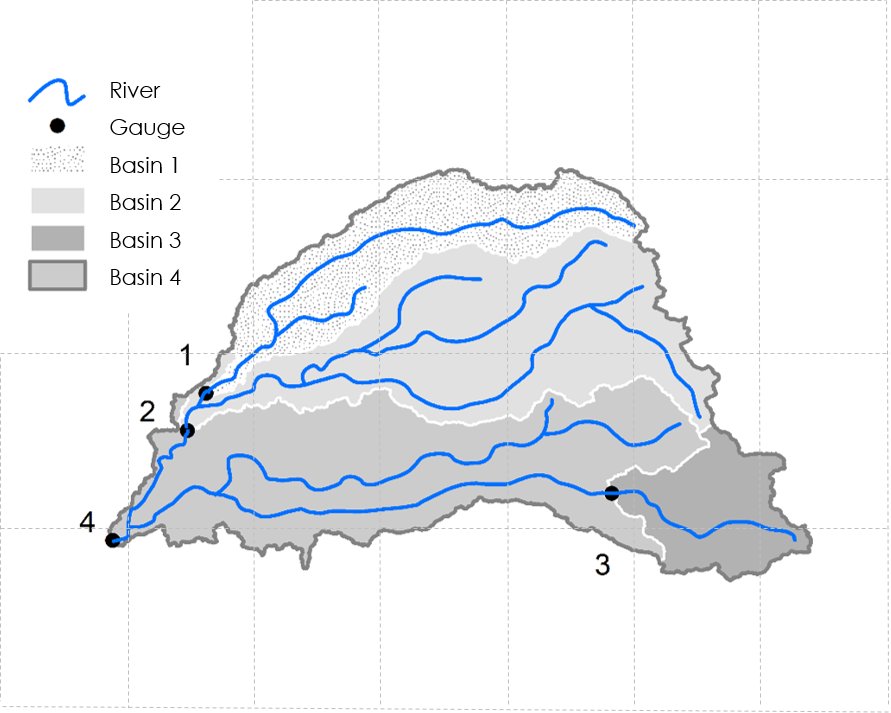
\includegraphics[width=\linewidth]{plots/ch1_pub_problem.png}
		\caption{PUB Problem}
		\label{fig:sub2}
	\end{subfigure}%
	\begin{subfigure}{.5\textwidth}
		\centering
		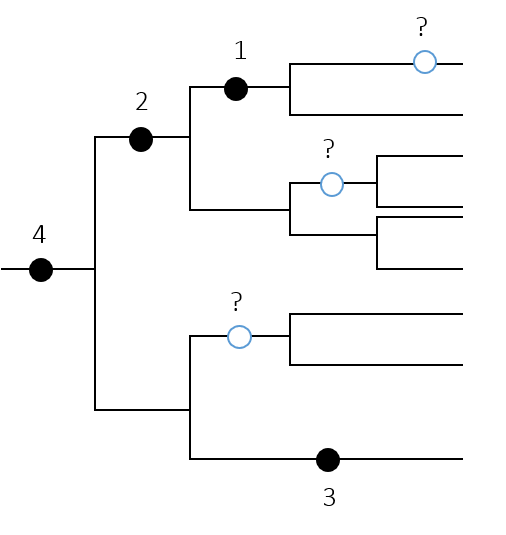
\includegraphics[width=0.74\linewidth]{plots/ch1_pub_schematic.png}
		\caption{PUB Schematic}
		\label{fig:sub1}
	\end{subfigure}
	\caption{The predicting ungauged basins (PUB) problem. This dissertation focuses on predicting unimpaired flows at ungauged locations from other gauges on the network. Predictor variables include climate and basin characteristics.}
	\label{fig:pubproblem}
\end{figure}

Predicting and forecasting hydrology at ungauged sites promotes better management of water and the environment \cite{sivapalan2003iahs}. It is
important for the sustainable management of river basins, integrating economic, social and environmental perspectives \cite{sivapalan2003prediction}, flood protection, water supply and drought management, solving water quality issues \cite{hrachowitz2013decade}, and to serve as inputs for other models. 

%----------------------------------------------------------------------------------------------------------------------------------------------------------------------------------------------------------
\section{Terms \& Definitions}
This dissertation investigates the relationships between the response variable: ``unimpaired flow'' and the predictor variables: climate and basin characteristics. Before continuing, it is useful to know how unimpaired flow is defined. Unimpaired flow is the flow that is produced by the basin in its current state, but, without dams and diversions \cite{cadwruf2016}. Unimpaired flow calculations are used mostly in places where dams have created major changes to the natural flow regime. It is often calculated by a simple accounting of water in the system (Figure \ref{fig:unimpairedflow} and Equation \ref{eq:massbalance}).
\begin{equation}
	\label{eq:massbalance}
	q_{uf} = q_{out} - q_{imp} + q_{div} + \Delta S + q_{evap}
\end{equation}

Where $q_{uf}$ is unimpaired flow, $q_{out}$ is observed gauge data, $q_{imp}$ is imported flows, $q_{div}$ is diverted flows, $\Delta S$ is the change in storage, and $q_{evap}$ is the evaporation out of the system.  

\begin{figure}
	\centering
	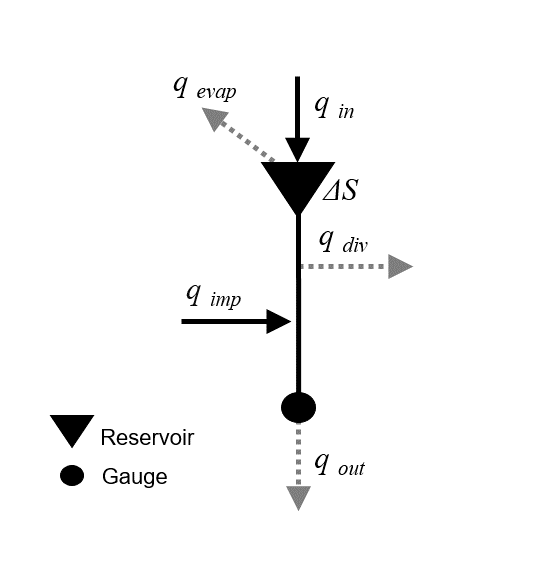
\includegraphics[width=7cm,trim={0 1cm 0 1cm},clip=true]{plots/ch1_unimpaired_flow.png}
	\caption{Calculating unimpaired flow. Unimpaired flow is calculated by adding back in diversions, subtracting imports, accounting for change in storage and evaporation caused by the reservoir.} 
	\label{fig:unimpairedflow}
\end{figure}

In contrast, ``natural flow'' is the runoff produced by a basin in its pre-development state prior to any human alterations \cite{poff1997natural}. The differences between unimpaired flow and natural flows are usually driven by effects of levees, upland land use, wetlands, and groundwater. This study, however, was only concerned with unimpaired flow; the models were built with unimpaired flow data from the California Data Exchange Center (CDEC), and the predictor variables are taken from various sources discussed in appendix \ref{a:data}. See appendix \ref{b:terms} for terms and concepts used in statistical learning. 

%----------------------------------------------------------------------------------------------------------------------------------------------------------------------------------------------------------
\section{Literature Review}

%-----------------------------------------------------------------
\subsection{Hydrologic Modeling}
Hydrologic models in PUB can be classified as \textit{mechanistic} (physical process-based, causal) or \textit{empirical} (statistical, purely stochastic) \cite{guisan2000predictive} (Figure \ref{fig:hydmodelclasses}). All modeling techniques assume that the past is a reasonable guide to the future, and that data from one basin is a useful guide to understanding hydrological responses at another basin \cite{sivapalan2003prediction}. But, each approach sacrifices some generality, realism, cost, and precision for better understanding, predicting, and managing natural resources \cite{levins1966strategy, klemes1982empirical}. 

 \begin{figure}
	\centering
	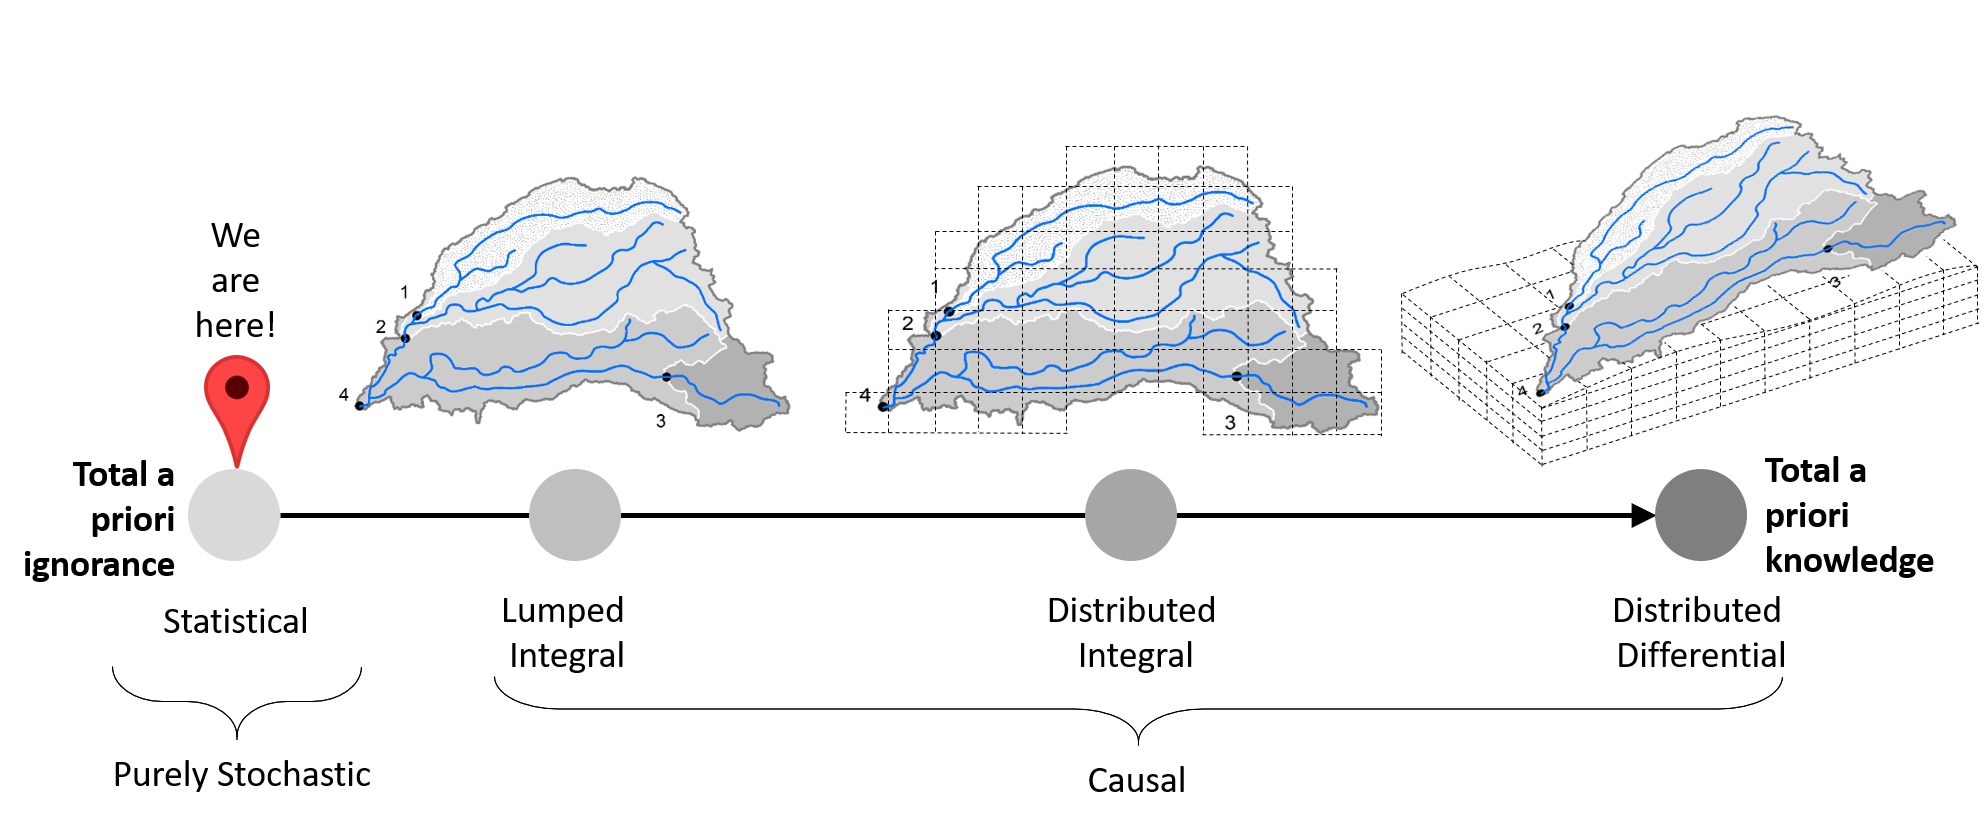
\includegraphics[width=16.51cm,trim={0 0 0 1.75cm},clip=true]{plots/ch1_hyd_model_classes.png}
	\caption{The different classes of hydrologic models. The hydrologic modeling field has been moving from total a priori ignorance to total a priori knowledge of the system. With the increase in computing power and the development of statistical learning methods, hydrologist can now re-visit predicting hydrologic conditions with purely stochastic methods.} 
	\label{fig:hydmodelclasses}
\end{figure}

Hydrologists have used both mechanistic and empirical models to capture complex runoff processes; since the mid-19\textsuperscript{th} century, with the employment of the \textit{rational method}, empirical relationships have been used in rainfall-runoff modeling \cite{beven2011rainfall}. Engineers developed the rational method in response to problems in which the design discharge was of major concern (i.e., urban sewer, land reclamation drainage systems, and reservoir spillway design) \cite{todini1988rainfall}. This method, based on the concept of concentration time, calculates runoff by simply multiplying a runoff coefficient by rainfall intensity and the basin's drainage area. It is applicable only to small or mountainous catchments where the rainfall duration normally exceeds the basin's concentration time, the time it takes for the entire basin area precipitation to reach the basin's outlet as discharge. 

To address more complexities in rainfall duration, basin size, and non-uniform characteristics, other methods emerged. In the 1930s, the \textit{unit hydrograph} method was developed \cite{sherman1932streamflow}. In the 1950s, mathematical techniques such as Z, Laplace or Fourier transforms led to the derivation of response functions from the analysis of input and output data \cite{dooge1973linear}. In the 1960s, grander approaches emerged to model the physical processes of the hydrologic cycle. Models increased in complexity over time and often lacked realistic parameter estimates, leading researchers to other ambitious mechanistic modeling efforts \cite{todini1988rainfall}. These models require considerable field input data collection and model calibration to obtain basin-specific parameters \cite{singh2005watershed}. Unfortunately, as mechanistic models increase in complexity, it is unclear if hydrologic predictions improve commensurately \cite{beven2011rainfall}. 

Our incomplete understanding of the process \cite{hrachowitz2013decade}, poor understanding of where water goes when it rains, what flow path it takes to the stream, and the age of the water that emerges in the channel \cite{sivapalan2003prediction} make PUB a difficult problem to model. Spatio-temporal heterogeneity of climate and basin characteristics create a \textit{uniqueness-of-place} issue, and there is a lack of agreement on what is a suitable regionalization technique for this problem  \cite{hrachowitz2013decade}. 

Without a unifying approach, and considering the increasing availability of environmental data, in the past two decades, more sophisticated statistical learning models have been applied to rainfall-runoff modeling. In juxtaposition with physical or semi-physical models, machine learning models learn from the data itself, with no assumptions as to the underlying process.

%-----------------------------------------------------------------
\subsection{Statistical Learning}
Artificial intelligence has gone through the ages of speculation (1940s), dawn, business, and bulldozer age \cite{winston2010class}. In the bulldozer age, with seemingly unlimited computing capacity, machines process more abundant data much like a bulldozer processes soil. Recent advances in reinforcement learning, one-hot learning (where machines learn from the first example), learning in sparse spaces, and the integration of thinking, perception, and action (rather than viewing them separately) are moving us away from the bulldozer era \cite{winston2010class}. See appendix \ref{c:history} for a brief history of statistical learning. However, the application of these newer techniques to water resources problems is slow. 
%Therefore, the literature reviewed in Section \ref{mlinciveng} is solely on computationally-intensive methods. 

% Theorists in statistical learning have made progress in developing methods, especially in supervised machine learning. However, if a statistical learning method works particularly well for one data set, it may be that the problem was defined in a space rich with solutions \cite{winston2010class}. That is, other statistical learning methods also could produce good results. Therefore, the merits of finding a solution may be due to either the statistical learning method or the problem's characteristics. Researcher can apply multiple statistical learning methods. 

We can group the statistical learning methods developed in the bulldozer age into seven main categories: \textit{supervised machine learning}, \textit{regression family}, \textit{time series analysis}, \textit{geostatistics}, \textit{multi-variate analysis}, \textit{unsupervised machine learning}, and other methods. Supervised machine learning methods are more generally used for predicting a variable in the past where no equation is needed to represent the model. In contrast, the regression family of methods are used when the purpose is more \textit{inference} than \textit{prediction}, and equations, or more specifically the coefficients of the variables in the equations, are of interest. Time series analysis is most suited to prediction problems where the time component is of interest (e.g., problem of extrapolating to the future), as opposed to geostatistics, which is mainly concerned with the spatial component of the data. Under pattern recognition problems sets, multi-variate analysis and unsupervised machine learning methods find natural groupings in the data. Other methods handle networks, text, patterns caused by latent factors, and relationships between variables, which generally don't apply to problems in water resources. Lastly, in descriptive methods, we use measures of center (e.g., mean and median), measures of spread (e.g., range, standard deviation, and quantiles), and the distribution of a variable as a way to describe the data. 

Taxonomies, like the one shown in Figure \ref{fig:modelsel}, help guide the user through a discovery process. Its goal is for the user to be able to identify an object of interest without prior knowledge of its existence. In statistical learning, method or model selection is iterative and should follow the \textit{generate-and-test} approach. So, any guide to model selection should be considered only a heuristic, meaning as a general rule it will recommend appropriate methods, but may fail sometimes. 

%\afterpage{% Insert after the current page
%	\clearpage
%	\KOMAoptions{paper=25.5in:11in,pagesize}
%	\recalctypearea
%
%	\begin{figure}
%		\centering
%   		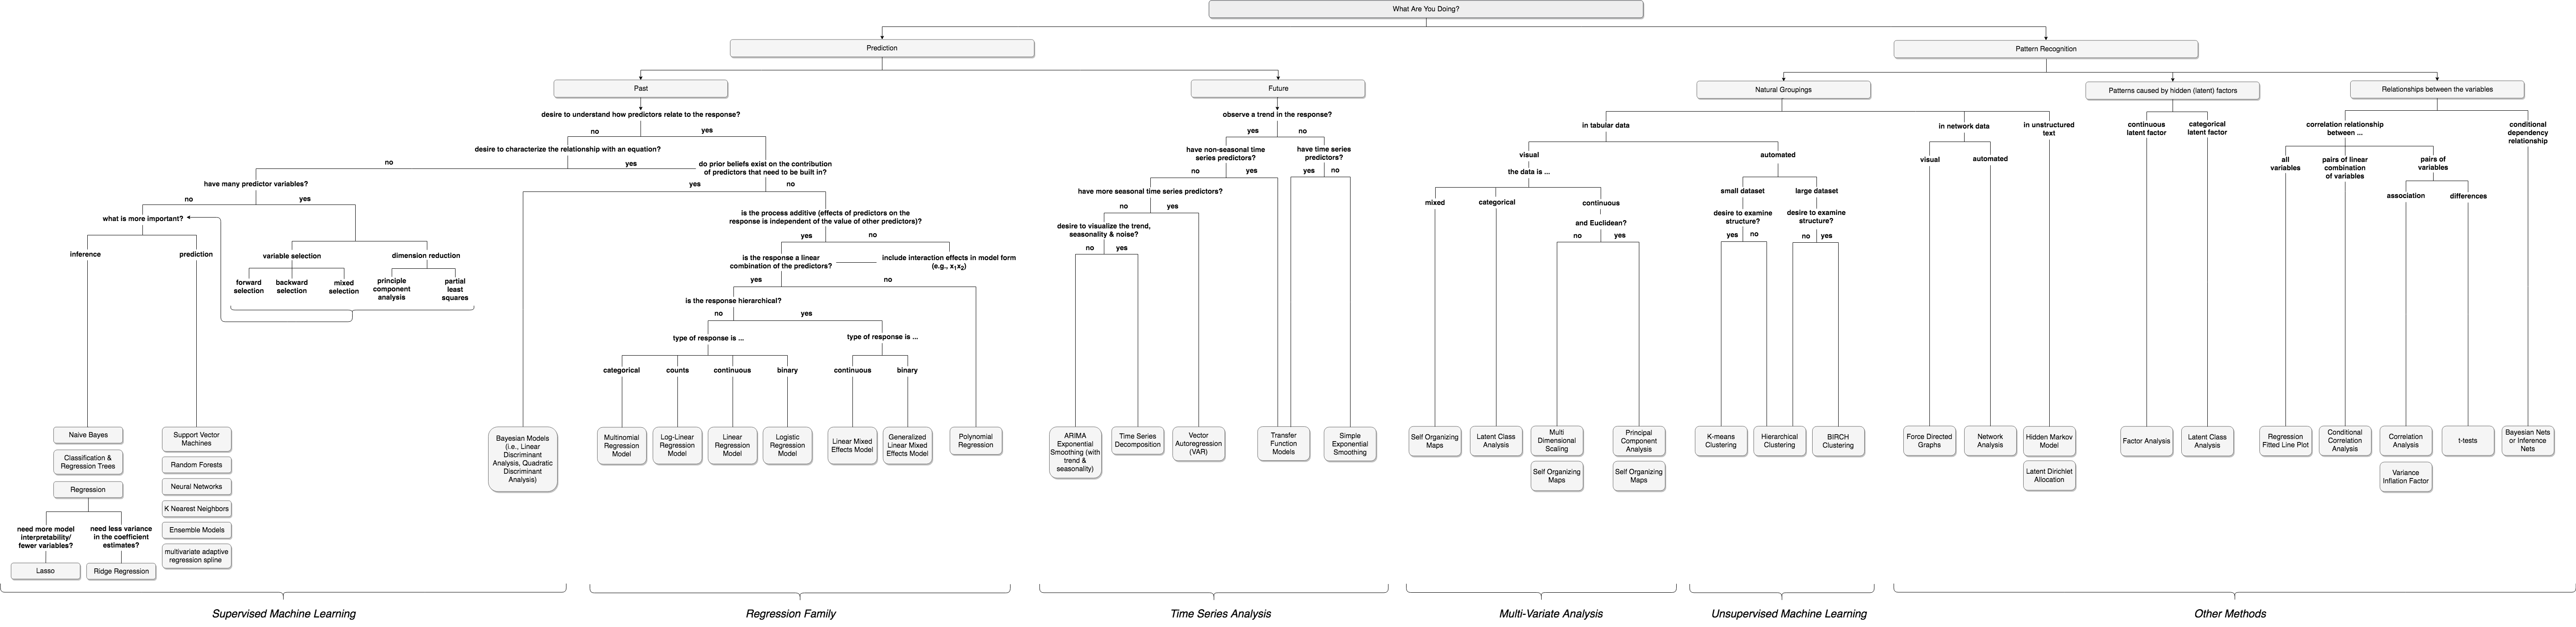
\includegraphics[width=25.5cm,trim={0 0 0 0},clip=true,keepaspectratio]{plots/model_selection.jpg}%
%   		\caption{What are you trying to do?} 
%		\label{fig:modelsel}
%	\end{figure}
%
%	\clearpage
%	\KOMAoptions{paper=A4,pagesize}
%	\recalctypearea
%}

%\begin{figure}[p]
%    \vspace*{-1in}
%    \makebox[\linewidth]{
%        \includegraphics[width=1.3\linewidth]{plots/model_selection_pages.pdf}
%    }
%    \caption{What are you trying to do? Heuristic guide for model selection.}
%\end{figure}

\begin{figure}
	\centering
	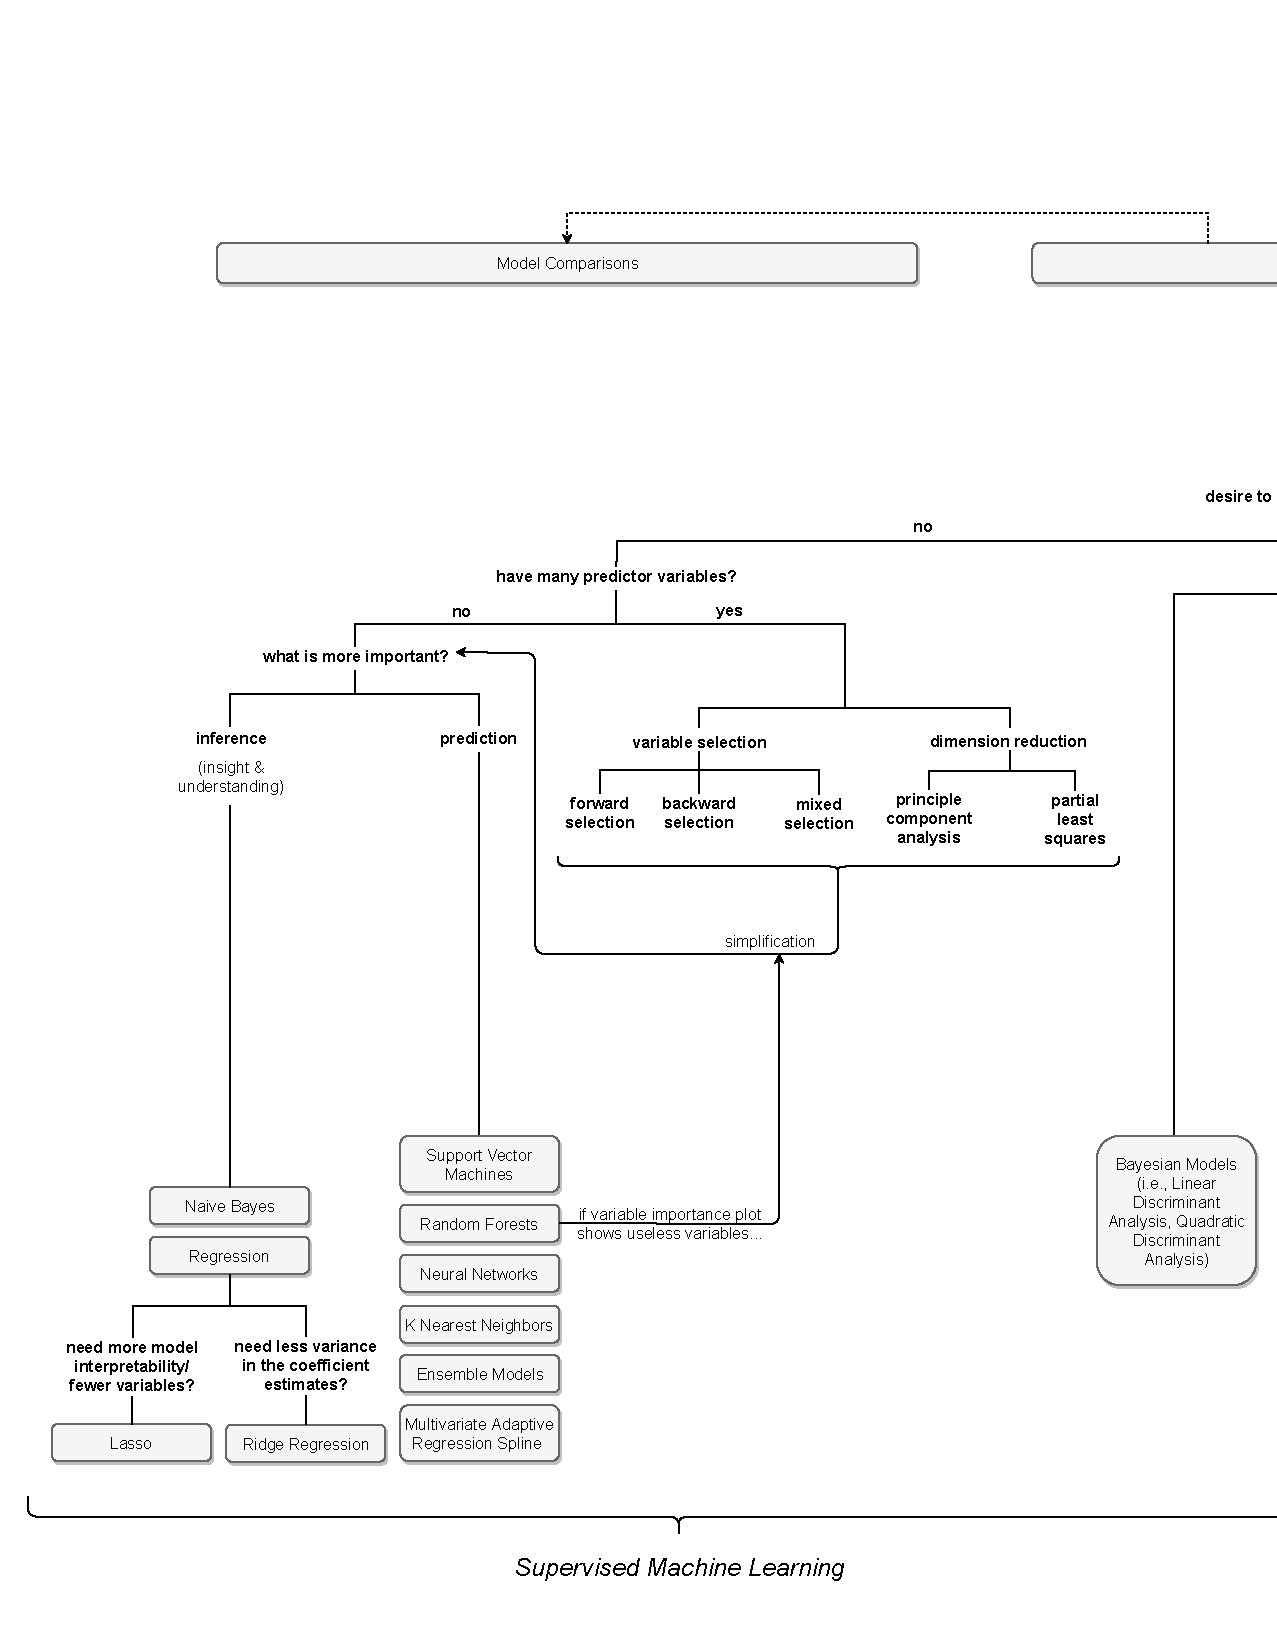
\includegraphics[width=\linewidth,trim={0 0.5in 0 0.8in},clip=true, page=1]{plots/ch1_statsflowchart.pdf}
	\caption{What are you trying to do? Heuristic guide for model selection.} 
	\label{fig:modelsel}
\end{figure}

The hydro-informatics literature shows that the techniques presented in the heuristic guide are aiding civil engineers in the fields of: (1) hydrology: e.g., rainfall-runoff modeling and model calibration; (2) hydraulics: e.g., water levels in channels and reservoirs; (3) environmental water quality: e.g., temperature and groundwater heads; (4) urban water supply: e.g., water demand and water distribution networks; and (5) general data cleaning and anomaly detection. In the following sections, we will discuss the models suitable to the PUB problem. 

%-----------------------------------------------------------------
% \subsection{Statistical Learning in Civil Engineering} \label{mlinciveng}
% CHANGE THIS WHOLE SECTION, SO IT IS ORGANIZED BY IDEAS NOT PEOPLE!!!!!!!

%Possible applications of statistical learning methods in water resources include the following: %CITATIONS COMING!!!
%
%\begin{itemize} % citations where available
%	\item Rainfall-runoff modeling: streamflow dis-aggregation or forecasting 
%	\item Building an assisting surrogate model in calibration of a rainfall-runoff model
%	\item Auto-calibration and uncertainty estimation methods
%	\item Modeling river stage-discharge relationships
%	\item Cleaning up anomalies in data: (cite Nate Chaney's work with SSURGO,  step like patterns in temperature from rounding observed data.) 
%	\item Simulating runoff, sediment and nutrient loadings from a watershed
%	\item Modeling rainfall-runoff processes intelligent controller for realtime management
%	\item Control of water levels in channels
%	\item Model-based optimal control of a reservoir
%	\item Forecasting the groundwater heads in an aquifer
%	\item River temperature prediction
%	\item Rainfall forecasting
%	\item Water demand forecasting
%	\item Flood forecasting
%	\item Predicting scour depth at culverts
%	\item Pipe deterioration models
%	\item Optimizing operations of a water distribution network 
%\end{itemize}

% rainfall-runoff modeling
% Can you break up these citations to provide a little more info about their contributions? If not, I would actually suggest reducing the list to only the most essential citations, since the others don't add much understanding. deleted: dibike1999encapsulation, abrahart2000comparing 
%As \shortciteA{solomatine2008data} explain, most machine learning techniques applied to the rainfall-runoff problem use neural networks \cite{govindaraju2013artificial}. Other studies use support vector machines \cite{lin2006using} and tree based algorithms \cite{galelli2013tree}. 
%
%% As \shortciteA{solomatine2008data} explain, most machine learning techniques applied to the rainfall-runoff problem use neural networks \cite{minns1996artificial, dawson1998artificial, tokar1999rainfall, hsu2002self, hu2007rainfall, abrahart2007timing, govindaraju2013artificial}. Other studies use support vector machines \cite{asefa2006multi, lin2006using}, and tree based algorithms \cite{iorgulescu2004nonparametric, galelli2013tree, bonniethesis}. 
%
%% flood forecasting
%\citeA{han2007flood}, \citeA{yu2004ec}, and \citeA{bray2004identification} used \textit{support vector machines} (SVMs) for flood forecasting. The applications of SVM in regression of time series is still in its infancy. Such studies show that advances are putting SVMs generally on par with neural networks in terms of model performance. 
%
%\citeA{han2007flood} shows a peculiar behavior of the SVM where lighter rainfall would generate unrealistic hydrographs that would increase to an equilibrium point rather than having the characteristic skewed bell shape. This contradicts the physical principle that limited rainfall cannot generate an unlimited flow. However, the model performs well given the data it has trained and was tested on \cite{han2007flood}. 
%
%\citeA{yu2004ec} used SVMs for real-time hydrologic forecasting. In this study, 16 years of daily data informs the learning or phase space reconstruction and the last year of record is used for a 1-lead day prediction. One problem with SVMs is their difficulty in dealing with a large training record, which is required in chaotic time series analysis. To make SVMs more suitable to such problems, a decomposition method can be applied, which is demonstrated \cite{yu2004ec}. 
%
%\citeA{bray2004identification} explored the relationships among various model structures, kernel functions (e.g., linear, polynomial, radial basis, and sigmoid), scaling factor, model parameters (i.e., cost C and epsilon) and composition of input vectors in the development of the SVM. 
%
%\citeA{gautam2001rainfall} proposes an adaptive neuro-fuzzy system with autoregressive exogenous input (ARX) structure which was capable of reasonably producing the hydrograph shape and was able to maintain a good representation of the overall water balance as well as the general flow pattern. Its excellent performance for one-step prediction shows that it will be very valuable for real-time forecasting and control of floods \cite{gautam2001rainfall}.

%% decision making
%\citeA{ames2005using} used \textit{Bayesian networks} to model water management decisions in complying with phosphorous loadings in a river. This study estimated the probability of meeting legal water quality requirements for phosphorus in a creek under several management scenarios and estimated the probability of increased recreational use of the reservoir on the creek and subsequent revenue under these scenarios. The Bayesian networks framework served as a structured means for capturing the probability that management activities will have the desired effect \cite{ames2005using}.
%
%% uncertainty estimation
%\citeA{shrestha2009assessing} used the UNcertainty Estimation based on Local Errors and Clustering (UNEEC) method for assessing total model uncertainty (i.e., model error in reproducing observed historical river flow data). The UNEEC method is a data driven technique that consists of clustering, estimation of the probability distribution of error, and building the model of the probability distribution of error \cite{shrestha2009assessing}.
%
%% time series forecasting
%\citeA{alvisi2007short} used an auto-regressive moving average (ARMA) model to forecast water demand. Since operational decisions have to be based on the
%expected future demands for water, rather than just the present known requirements, it is necessary to develop a short-term, demand-forecasting procedure. Trends, seasonality, and general periodicities are usually found in these type of time-series, which make them ideal candidates for ARMA models. 

%-----------------------------------------------------------------
\subsection{Suitable Statistical Modeling for Hydrologic Data}

Precipitation feeding into a stream needs to satisfy soil moisture deficits along its flow path before it produces runoff. In other words, the soil needs to ``fill" up to a certain threshold before it can ``spill" \cite{spence2006hydrology}. Therefore, a \textit{threshold behavior} is frequently discussed as influencing local, hillslope and catchment scale runoff generation processes \cite{zehe2008threshold}. This physical phenomenon may be why most successful machine learning techniques currently applied to the rainfall-runoff problem use artificial neural networks (e.g., \citeNP{minns1996artificial, dawson1998artificial, tokar1999rainfall, hsu2002self, hu2007rainfall, abrahart2007timing, govindaraju2013artificial}). In artificial neural networks, at each node the weighted sum of all inputs are passed through a non-linear activation function. Much like the neurons in our brains, there is a threshold that determines if the neuron will ``fire". 

The same effect can be replicated with tree based algorithms where models are built with a series of binary splits on the predictor variables (e.g., \citeNP{iorgulescu2004nonparametric, galelli2013tree, bonniethesis, worland2018improving}). Papers in which the number of basins in the study are fairly small suffer when forming the test/train or calibration/validation split. Usually, in these studies the data for one whole basin is not held out when training; in other words, the models are able to learn from a partial record from the basin of interest. Although this approach seems to be valid for rainfall-runoff modeling in the current literature, it does not comply by the test set requirements in the PUB problem where no data from the basin in the test set is available to the model. In contrast, when the datasets are large (e.g., studies done on the the GAGESII dataset, a massive USGS hydrologic data set), this problem is less pronounced. Some studies employ a random test/train split which is not appropriate when the dataset is correlated. We will discuss this concept further in chapter \ref{ch4:resampling}. These studies also employ a pre-modeling split on the dataset when classifying basins as ``impaired" vs. ``reference" basin. This imposes a subjective top split in the data and homogenizes the basins in the study; the reference basins are usually smaller headwater basins with low flows. As such, and rightly so, these models fail to make accurate predictions when extrapolating to basins lower in the network, with higher flows, since the model was denied information such information.  

More recently, studies have turned to support vector machines (SVM) \cite{asefa2006multi, lin2006using}, which initially were only applied to classification problems and have now been modified to accommodate regression problems (e.g., \citeNP{han2007flood, yu2004ec, bray2004identification} applied to flood forecasting). Such studies show that advances are putting SVMs generally on par with artificial neural networks in terms of model performance. However, the applications of SVM in time-series regression is still in its infancy; one study showed a peculiar behavior of the SVM where lighter rainfall would generate unrealistic hydrographs that would increase to an equilibrium point rather than having the characteristic skewed bell shape \cite{han2007flood}. Of course, this contradicts the physical principle that limited rainfall cannot generate an unlimited flow.

The difficulty in modeling lower flows is not unique to SVMs. Other modeling techniques (e.g., LM, GLMs, ...) suffer from the same problem given that the response, unimpaired flows, is a \textit{semi-continuous} variable. Semi-continuous data take non-negative values but have a substantial proportion of values at zero. The modeling of such ``clumped-at-zero" or ``zero-inflated"  data is challenging \cite{min2002modeling}. The following methods have been developed to solve this issue: 

\begin{itemize}
	\item Censored regression model: A censored regression, or Tobit, model assumes that the data comes from a single underlying Normal distribution, but that negative values are censored and stacked on zero \cite{tobin1958estimation}.
	\item Two-part models: As opposed to the Tobit model that allows the same underlying stochastic process to determine whether the response is zero or positive as well as the value of a positive response, two-part models allow the two components to have different parameters. Without assuming an underlying distribution,  \citeA{duan1983comparison} proposed a two-part model that uses two equations to separate the modeling into two stages. The first stage refers to whether the response outcome is positive (e.g., a binomial model). Conditional on its being positive, the second stage refers to its level (e.g., linear model).
	\item Compound Poisson exponential dispersion models: A model that uses a single distribution from the exponential dispersion family (i.e., Tweedie distribution) to analyze semi-continuous data. The distributions in this family have a given range of shape parameters ($1<\alpha<2$) which define a point mass at zero and a skewed positive distribution for positive values. 
\end{itemize}

As \citeA{min2002modeling} explain, other modeling methods exist to solve the problem of inflated zeros or other inflated boundaries (e.g., ordinal threshold, finite mixture, Neyman type A models). Unfortunately, these methods may require groupings that necessitate information loss, may overestimate the number of components when there is a lack of model fit, or employ methods where the mathematical and inferential advantages associated with the family of distributions are not available and are simply difficult to fit. As such, we will not discuss them here. 

In this thesis, we will be developing Linear Multivariate Regression (LM) as a first pass model. We will then develop Generalized Linear Regression (GLM), Tobit Regression (TR), Random Forest (RF), and Neural Network (NN) models. 

%----------------------------------------------------------------------------------------------------------------------------------------------------------------------------------------------------------
\section{Limitations \& Assumptions of Statistical Modeling}
Many hydrologists are skeptical of statistical modeling. \citeA{klemes1982empirical} warns modelers of the general limitations of empirical modeling, some of which are discussed here.

In search of ``better calculus'', the modeler may be in danger of \textbf{overfitting} (i.e., regarding noise in the data as information) \cite{klemes1982empirical}. However, resampling methods, when correctly applied, can illuminate differences between training and testing set performances \cite{friedman2001elements}.

Furthermore, empirical models must be regarded as \textbf{interpolation formulas}, and so, lack justification outside the range of underlying data sets \cite{klemes1982empirical}. The models in this study were fitted with data on the California Sierra Nevada mountainous basins, and some coastal, and southern California basins (Figure \ref{fig:map}). These training data sets mostly span the same hydrologic region (i.e., the United States Geological Survey Region No. 18). As such, the model may not be applicable to basins outside this spatial range as other hydrologic processes may dominate other basins. We can demonstrate this by observing the spatial variability (i.e., the coefficient of variation) in precipitation across the United States (Figure \ref{fig:coefvar}; \citeNP{dettinger2011atmospheric}). 

\begin{figure}[ht]
	\centering
	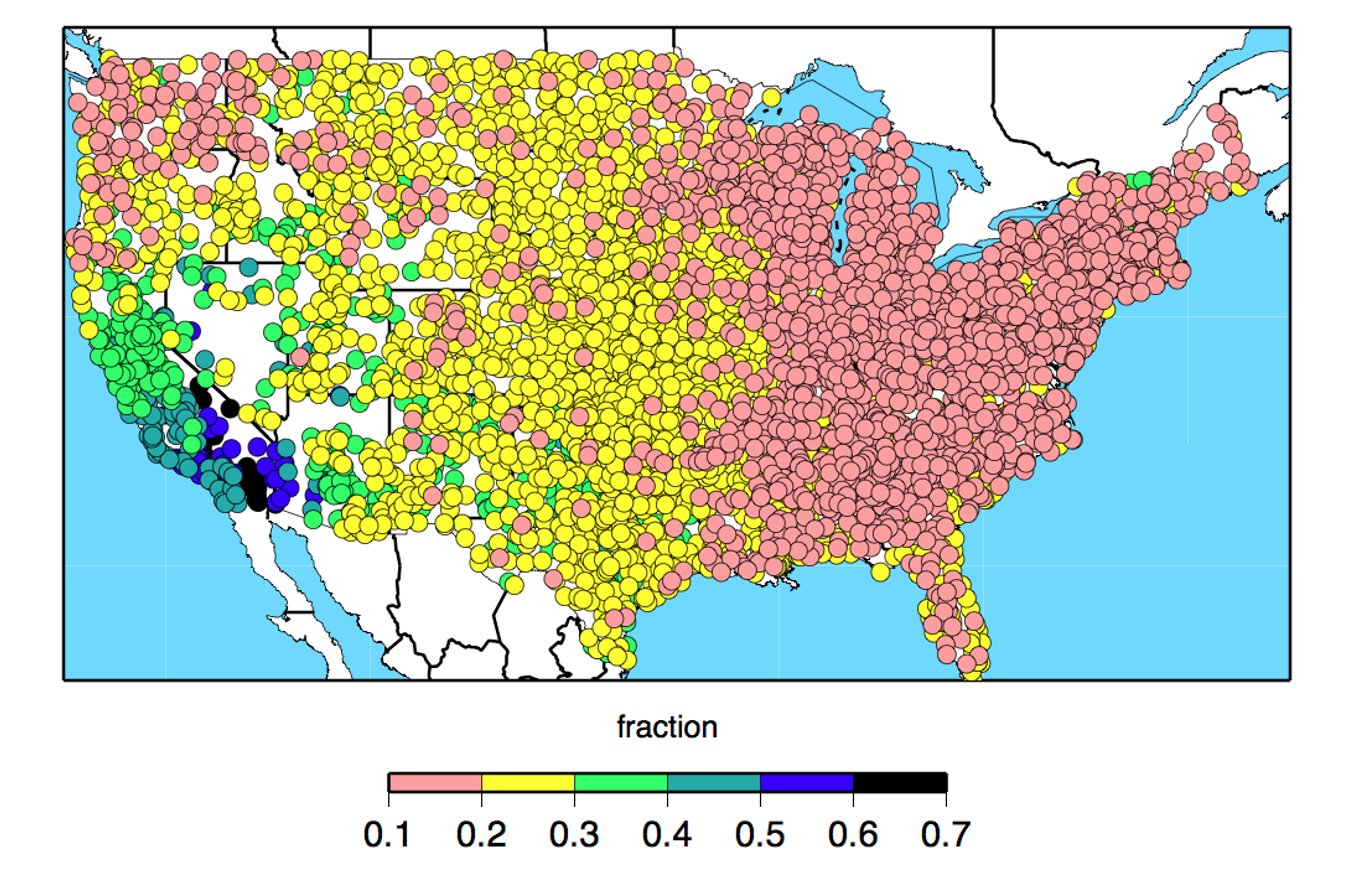
\includegraphics[width=0.8\textwidth,trim={0 0 0 0},clip=true]{Plots/ch1_coefficientofvariation.png}
	\caption{Coefficient of variation in total precipitation from 1951-2008. Reprinted from \protect\citeNP{dettinger2011atmospheric}}.
	\label{fig:coefvar}
\end{figure}

In addition to concerns with spatial extrapolation, there is temporal extrapolation. Climate change emposes \textbf{non-stationarity} in environmental variables like precipitation and temperature. Empirical models for flow should not be used to extrapolate beyond the limits of the variables the model observes or it will risk large errors. However, many advances in time-series analysis handle non-stationarity in data; one can reduce the process to a stationary one (i.e., trend seasonality and noise can be decomposed) or consider these processes as stochastic.
% Jay's comment: I have always thought that climate change makes empirical models riskier. But perhaps there are benefits of taking/modifying empirical models of warmer basins for todays cooler basins. 

Another downside is the \textbf{complexity in model structure}, especially in ensemble statistical learning methods, sometimes referred to as black-box models. If inference, or model parameters, are of interest, complex models introduce challenges. Dimensionality reduction methods (e.g., principle component analysis, partial least squares) and regularization techniques in regression (e.g., ridge, lasso, and elastic net) can help reduce the number of model parameters, and systematically produce simpler models \cite{friedman2001elements}. 

The essential \textbf{arbitrariness in the selection of the form} of an empirical model is another drawback \cite{klemes1982empirical}. Most studies report using one modeling method, which perhaps suggests that researchers are not employing more than one modeling method. Such a study could provide insights into the system by revealing the sensitivity of results to the algorithms employed. Therefore, the application and comparison of different machine learning models to the PUB problem was considered in this study. 

Lastly, some limitations are caused by the \textbf{nature of the algorithms} deployed. For example, regression-based random forest models make predictions by averaging predictions made by multiple regression trees. Therefore, the ensemble model limits the predictions it makes to the range seen in the training data; the predictions do not extrapolate to ranges not seen in the training data. In fact, averaging dampens the density function when we compare  observed to predicted data. This is especially problematic where the extreme tails of the distribution (i.e., floods and droughts) are of interest. Another example is that of the SVMs mentioned before that seem to perform poorly on low rainfall data. 

% some of these models get it right for the wrong reasons, and those few statistics are not reflective of how well a model does, two models can have the same statistics but perform vastly differently. 

%----------------------------------------------------------------------------------------------------------------------------------------------------------------------------------------------------------
\section{Conclusion} 
Generally, in statistical learning, applications lag behind advances in theory; the application of statistical learning theory to water resources problems is still in the bulldozer era, so, most models are computationally expensive. In the past two decades, in hydrology, statistical learning methods have been applied to modeling rainfall-runoff processes, predicting streamflow temperatures, sediment and nutrient loadings, forecasting the groundwater heads in an aquifer, or water demand among many others.

This chapter's main contribution is a heuristic guide to empirical model selection. Like a flowchart, it guides in selecting methods tailored to general purposes and limitations of various empirical modeling approaches. This guide should help in selecting from range of possible methods that are well suited to a problem at hand and give some comparative insights on these diverse methods. As a heuristic it works in most cases, but it is not comprehensive or applicable to all problems. 

In some cases, a wide range of empirical models can be employed, suggesting that no one single modeling method is useful across all locations, timescales, and problems. Also, despite their other limitations discussed in this chapter, these methods are much easier, faster, and less expensive to apply and study than mechanistic models. They are well suited to dynamic, non-linear and sometimes noisy data, especially when underlying physical processes are complex or not fully understood. In addition, the purpose of modeling is often to inform decision makers with adequate timing. For example, models need to be run during and just before flood events. Real-time applications require rapid computation, which statistical methods provide. The merits of statistical learning techniques, as a subset of empirical models, motivate their study in the following chapters.

This dissertation follows steps outlined in Figure \ref{fig:steps}. Chapter two compares two different data transformations that reflect our philosophical view of hydrology. Chapter three explores the effect of the loss functions on the model parameters and estimates. Chapter four compares different resampling methods for test error approximation. Chapter five discusses model development for non-stationary hydrologic processes. 

\begin{figure}[H]
	\centering
	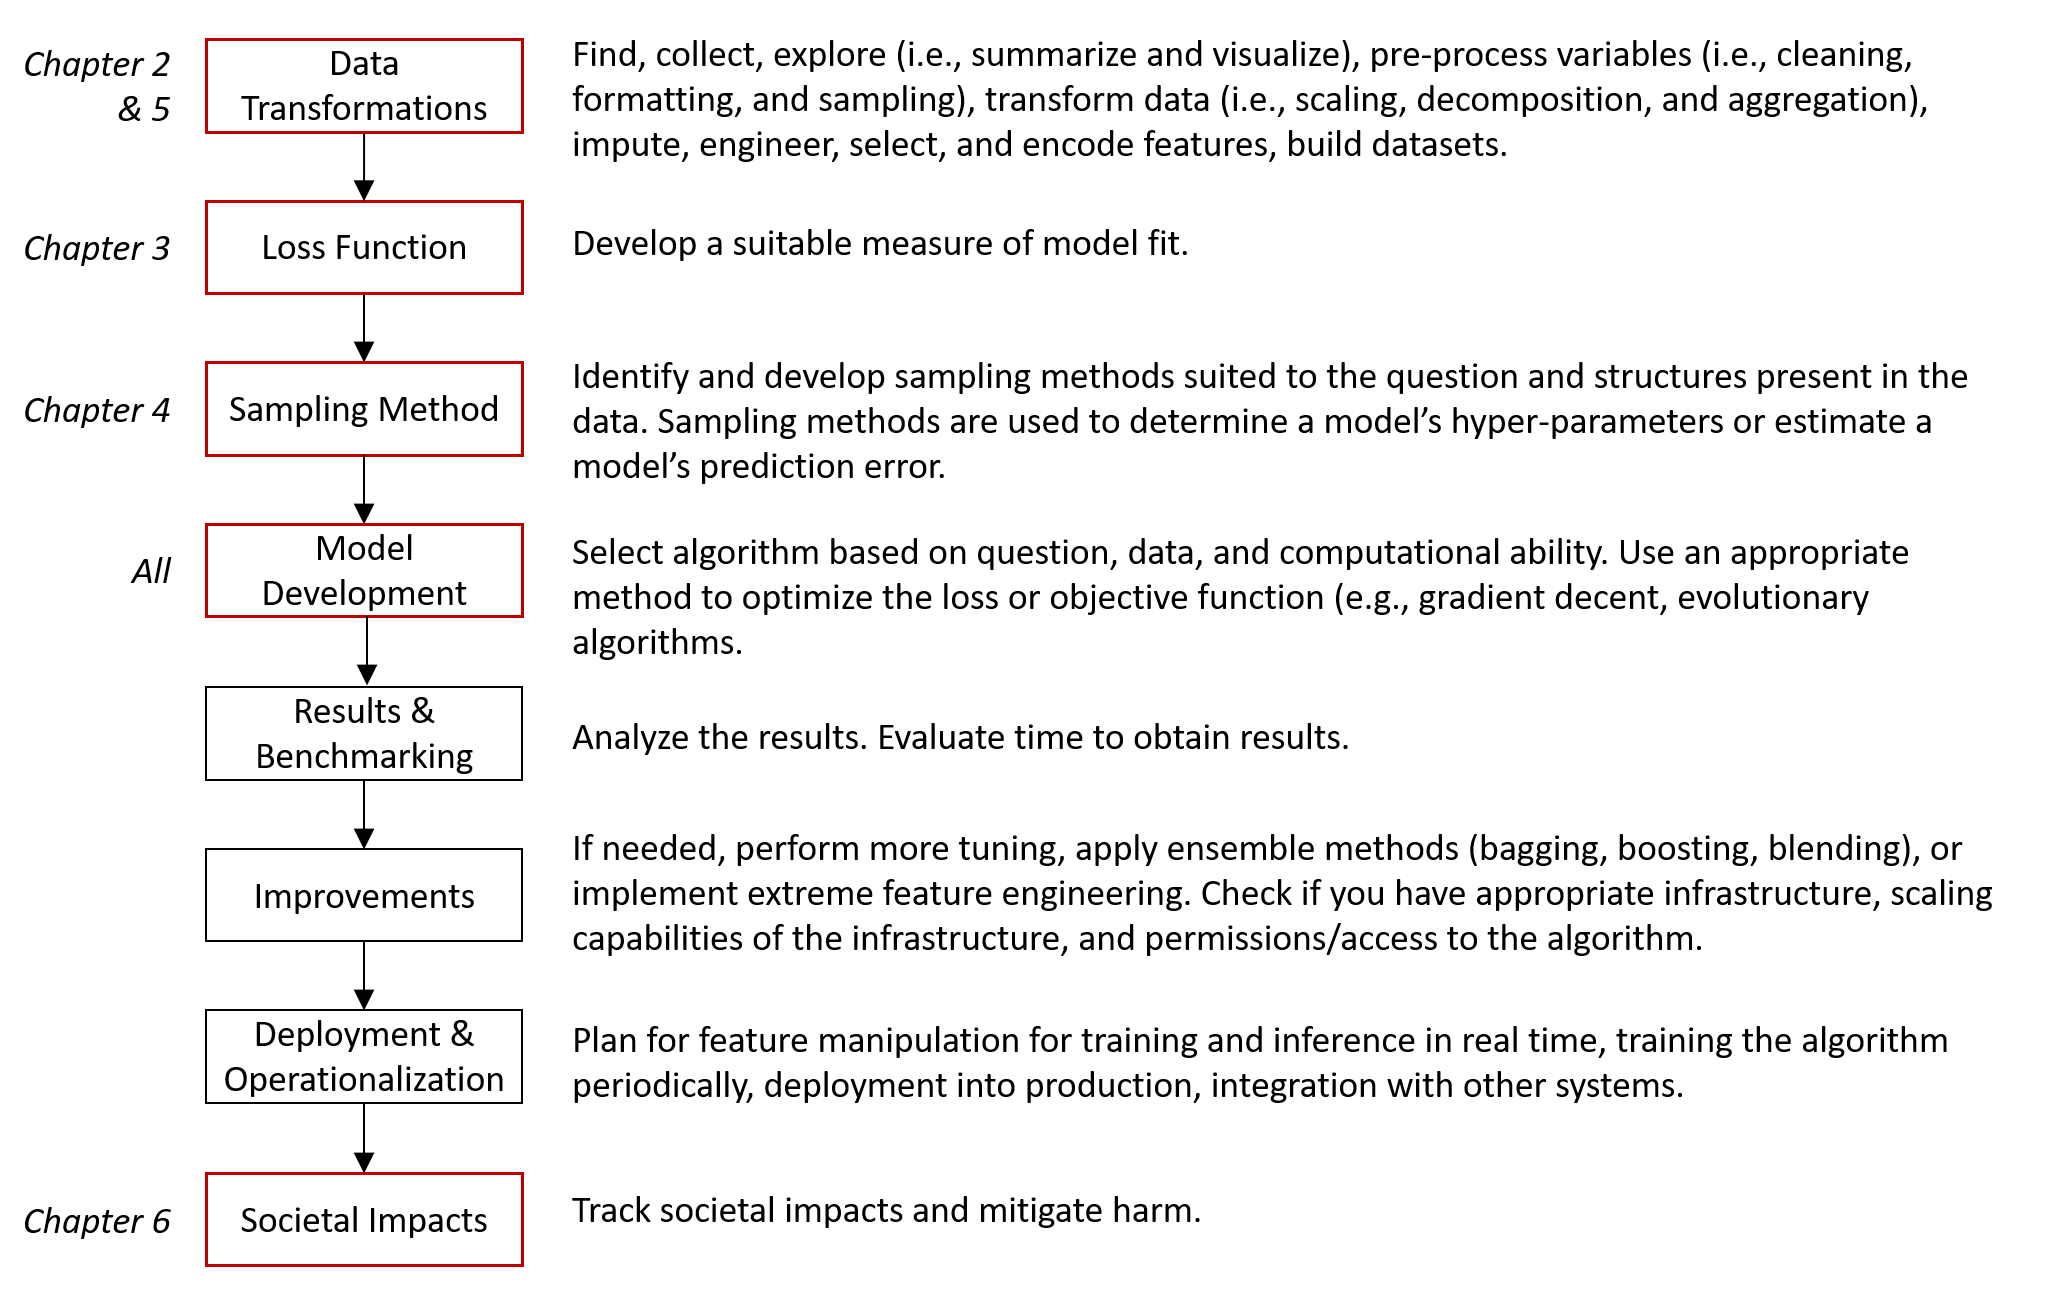
\includegraphics[width=\textwidth,trim={0 0 0 0},clip=true]{plots/ch1_diss_steps.png}
	\caption{Statistical learning steps. Adapted from \protect\citeNP{mlmastery2014, mindmap2017}. Each chapter of this dissertation discusses a unique step.} 
	\label{fig:steps}
\end{figure}

%\begin{enumerate}
%	\item Data: Find, collect, explore (i.e., summarize and visualize), pre-process variables (i.e., cleaning, formatting, and sampling), transform data (i.e., scaling, decomposition, and aggregation), impute, engineer, select, and encode features, build datasets.
%	\item Model: Select algorithm based on question and available data.
%	\item Loss or objective function: Develop a measure of model fit.
%	\item Optimization: Use an appropriate method to optimize the loss or objective function (e.g., gradient decent, evolutionary algorithms).
%	\item Tuning: Determine the model's hyper-parameters with cross-validation. There are multiple methods (e.g., grid search or random search) for optimal hyper-parameter specification. 
%	\item Results and Benchmarking: Analyze the results. Evaluate time to obtain results.
%	\item Improvements: If needed, perform more tuning, apply ensemble methods (bagging, boosting, blending), or implement extreme feature engineering.
%	\item Scaling: Check if the algorithm scales for expanding training datasets and in cases of inference.
%	\item Deployment and Operationalization: Plan for feature manipulation for training and inference in real time, training the algorithm periodically, deployment into production, integration with other systems.
%	\item Infrastructure: Check if you have appropriate infrastructure, scaling capabilities of the infrastructure, and permissions/access to the algorithm.
%\end{enumerate}

%Research objectives of this dissertation include:
%
%\begin{itemize}
%	\item \textit{Chapter 2, Data Transformations: Philosophical Views of Hydorlogic Modeling} - Present different data transformation techniques for hydrologic modeling that each represent a different philosophical view of hydrologic processes. 
%	\item \textit{Chapter 3, Rethinking Resampling Methods} - Describe how to more accurately estimate a model's prediction error with resampling methods when the data is structured. Structured data has internal correlation structures that need to be accounted for when resampling. 
%% \textbf{Questions}: How can we accurately estimate the model's prediction error with resampling methods when the data is structured? Structured data has internal correlation structures that need to be accounted for when resampling. \\
%	\item \textit{Chapter 4, New Loss Functions} - Encourage examination of off-the-shelf machine learning methods, specifically their default objective function. Identify some characteristics to consider when designing a loss function for machine learning algorithms. Examine how different loss functions perform when used to model hydrology. 
%% \textbf{Questions}: What are some characteristics one should consider when designing a loss function for machine learning algorithms? How do different loss functions perform when they are used to model hydrology? \\
%%What are some possible alternatives to the objective functions typically applied in off-the-shelf statistical learning techniques? These alternatives should be more suited to modeling extremes, which is usually where good management is more paramount in water resources. \\
%	\item \textit{Chapter 5, Modeling Methods} - Discuss the methods used for hydrologic modeling and their performance.  
%	\item \textit{Chapter 6, Climate Change Considerations} - Discuss data processing and modeling changes to incorporate a changing hydrology.
%	\item \textit{Chapter 7, Beyond McDonaldization: The ``Robotanization" of Agriculture} - Look to the impacts of statistical learning on our society and economy. Discuss how statistical learning is changing our society and what ``irrationalities" may it produce or take away that make it distinct from past mechanization. 
%% \textbf{Questions}: How is statistical learning changing our society? In other words, what ``irrationalities" may it produce that may have been non-existent in past mechanization, and what irrationalities may it take away? \\
%\end{itemize}




	

\chapter[Data Transformations]{Data Transformations: Two Philosophies on Hydrologic Processes} \label{ch2:transformations}
\chaptermark{Data Transformations}
\setlength{\epigraphwidth}{4.5in}
\epigraph{Science is what we know, and philosophy is what we don't know.}{Bertrand Russell, \textit{``Unpopular Essays''}, 1950}

%----------------------------------------------------------------------------------------------------------------------------------------------------------------------------------------------------------
\section*{Summary}
This chapter developed linear multivariate regression (LM), generalized linear regression (GLM), random forest (RF), and Neural Network (NN) models with a typical least squares loss function, of monthly unimpaired flows in 67 California basins. The best overall error (Bias-Corrected Coefficient of Determination, bR\textsuperscript{2}=0.92, Nash-Sutcliffe Efficiency, NSE=0.97) reflects the model's ability to capture monthly variations in flow. The NN with ``incremental basins" performed the best in the NSE criterion. Incremental basins are segments of the basin that have not been gauged, a concept discussed in this chapter. 

The test set error from ``leave one group out" (LOGO) cross-validation shows that model quality in predicting unimpaired flow is very spatially variable. LOGO cross validation and other resampling strategies are discussed in the next chapter. A comparison of different models concludes that the incremental basin approach to hydrologic modeling provides increasing benefits as the outlet of interest moves downstream in the gauge network. 

%Lastly, next steps and model improvement strategies are discussed.

%----------------------------------------------------------------------------------------------------------------------------------------------------------------------------------------------------------
\section{Introduction}
% add literature review here: klemes on double mass curves, 1922 varletes res opt, ripple method
%what is this chapter about, practical problems, literature, major contributions and structure
Unimpaired flows can be presented in two fundamentally different ways: (1) we can imagine each basin as a separate function that transforms its inputs (precipitation and snow) into runoff (or unimpaired stream flow). Here, we define each basin to be an ``aggregate" basin. Flows for these basins are simply the observed gauge values (Figure \ref{fig:aggbasins}); (2) we can imagine the basins as interconnected, and overlapping. One stream flows into another, like in a network, and so, some basins overlap. Here, we can define ``incremental" basins to be segments of basins that do not overlap. Flows for these basins are the amount that has not been observed by gauges in the network above the outlet of interest (Figure \ref{fig:incbasins}). Therefore, when modeling incremental flows, the network information is being preserved.

%\begin{figure}
%	\centering
%	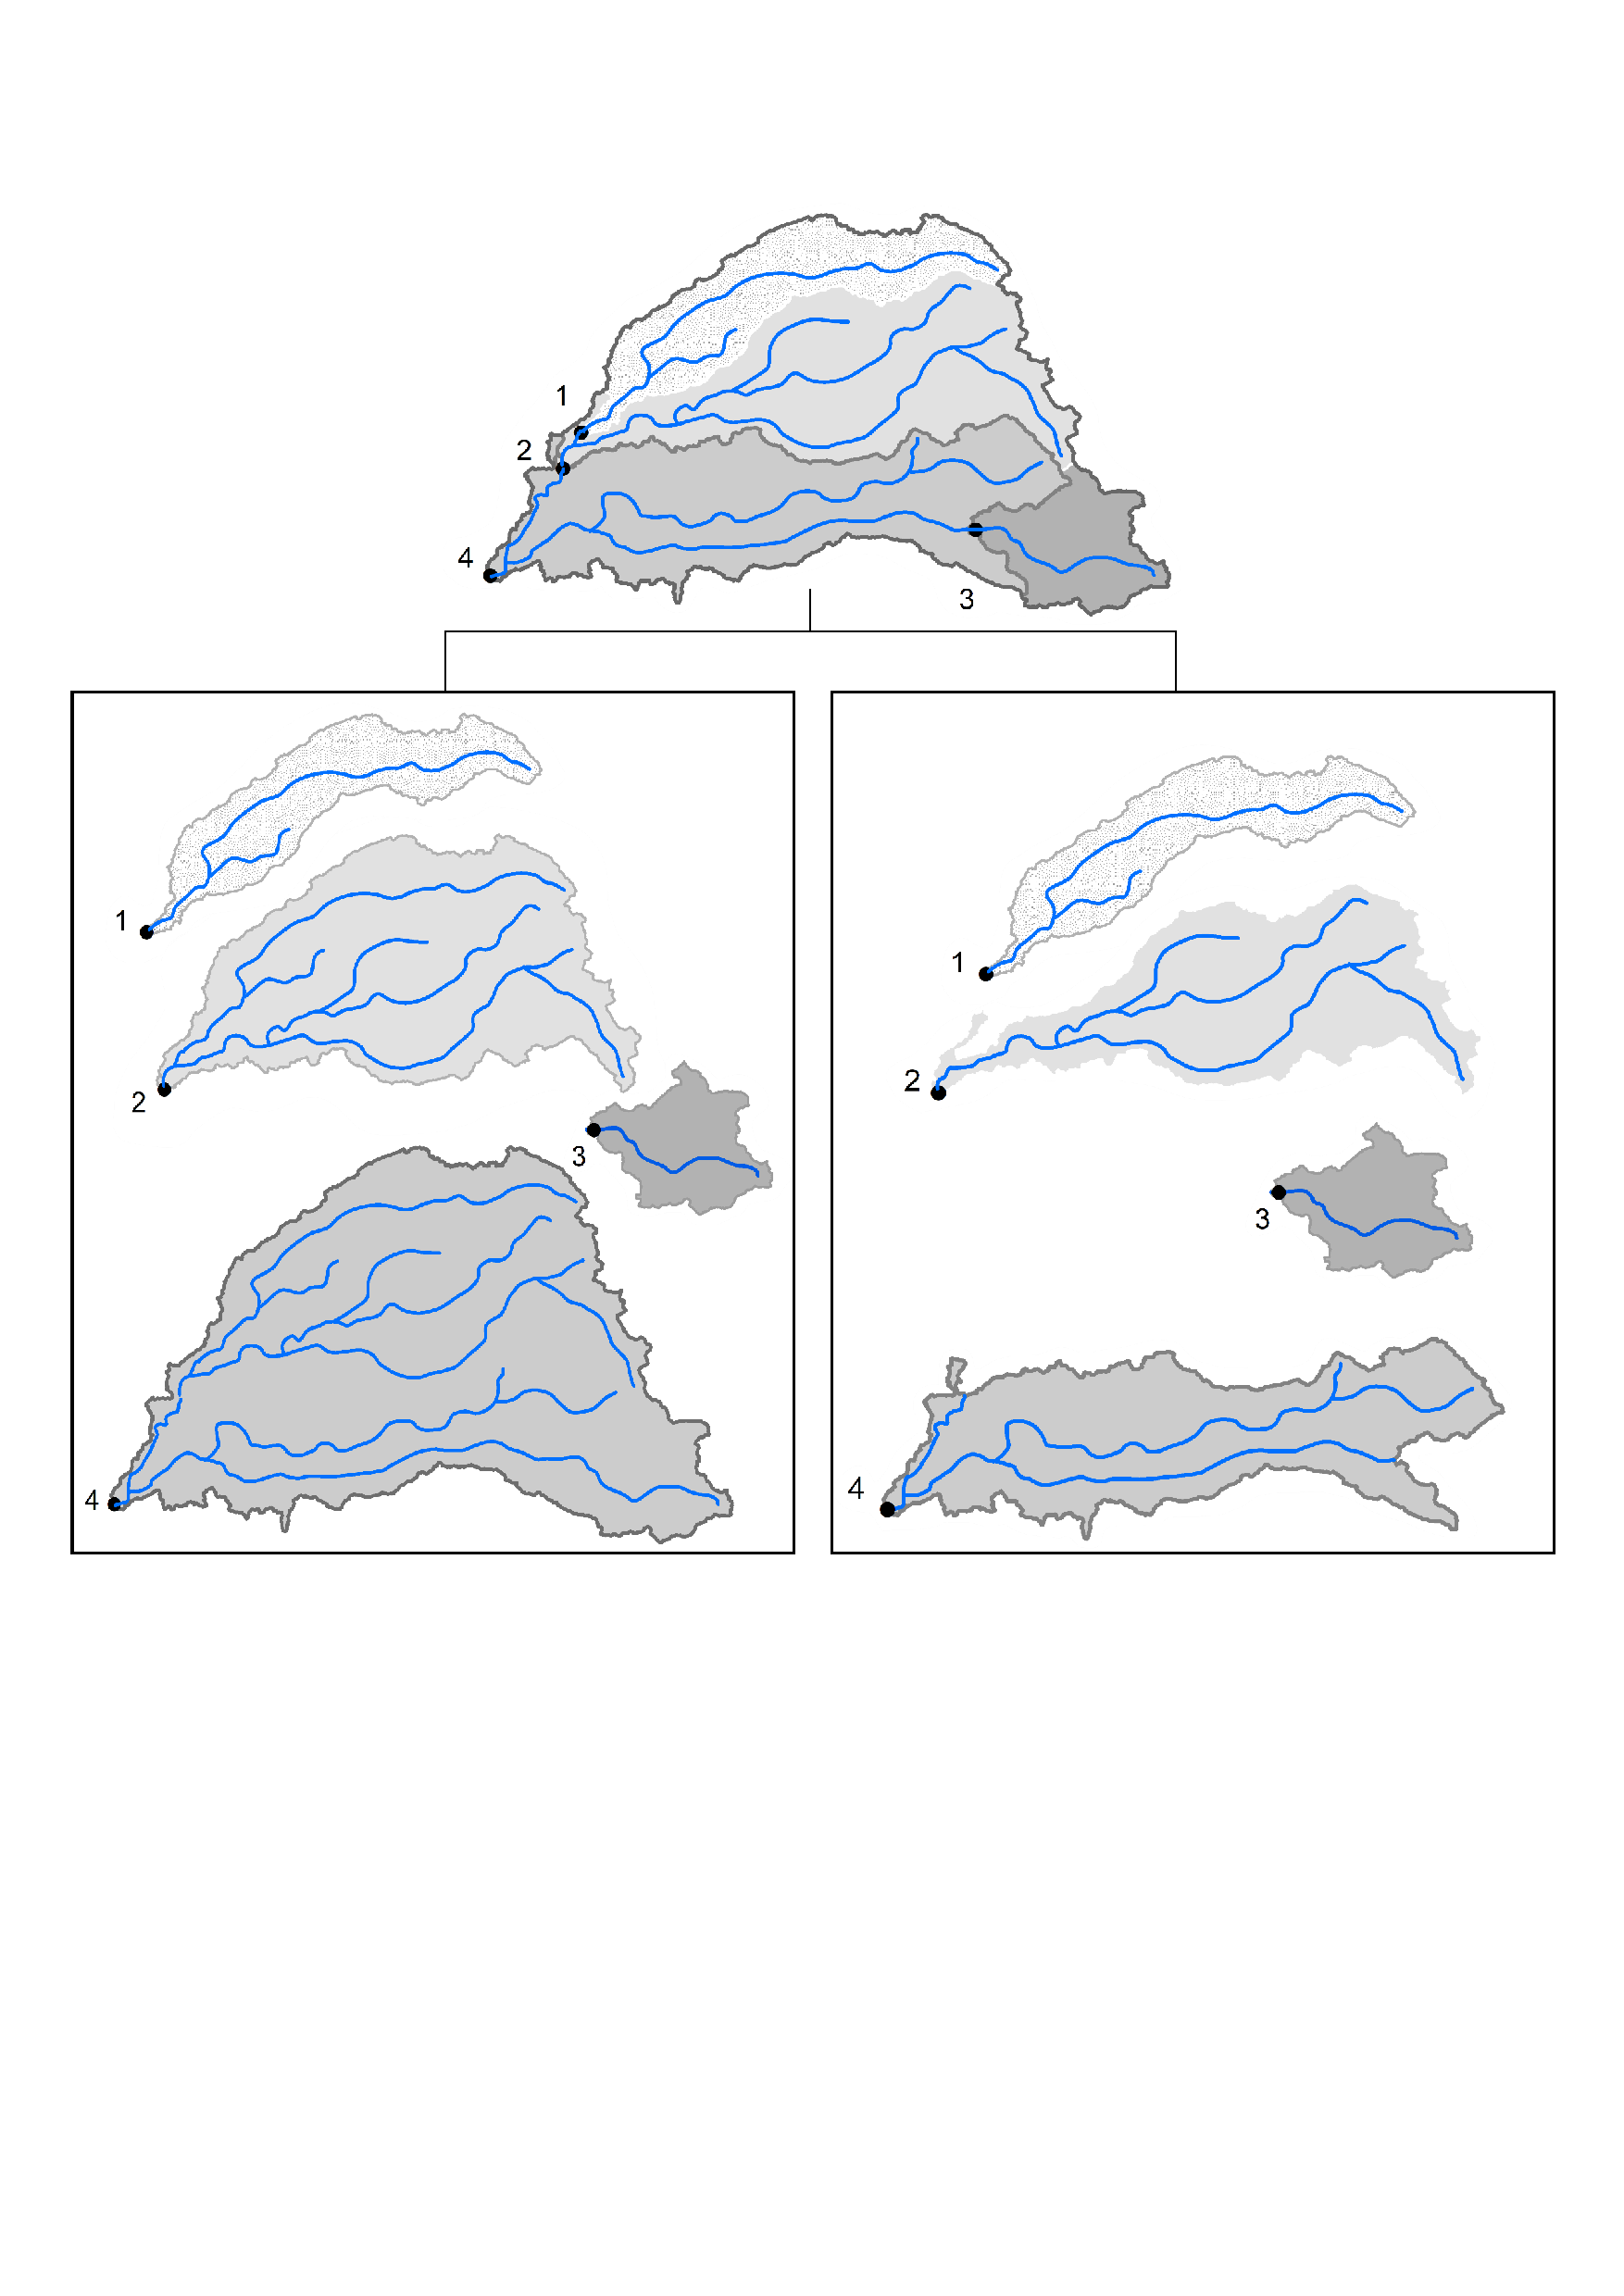
\includegraphics[width=16.5cm,trim={0 10cm 0 3cm},clip=true]{plots/agg_and_inc_basins.pdf}
%	\caption{Agg and Inc Basins} 
%	\label{fig:aggincbasins}
%\end{figure}

\begin{figure}
	\centering
	\begin{subfigure}{0.7\textwidth}
  		\centering
 		 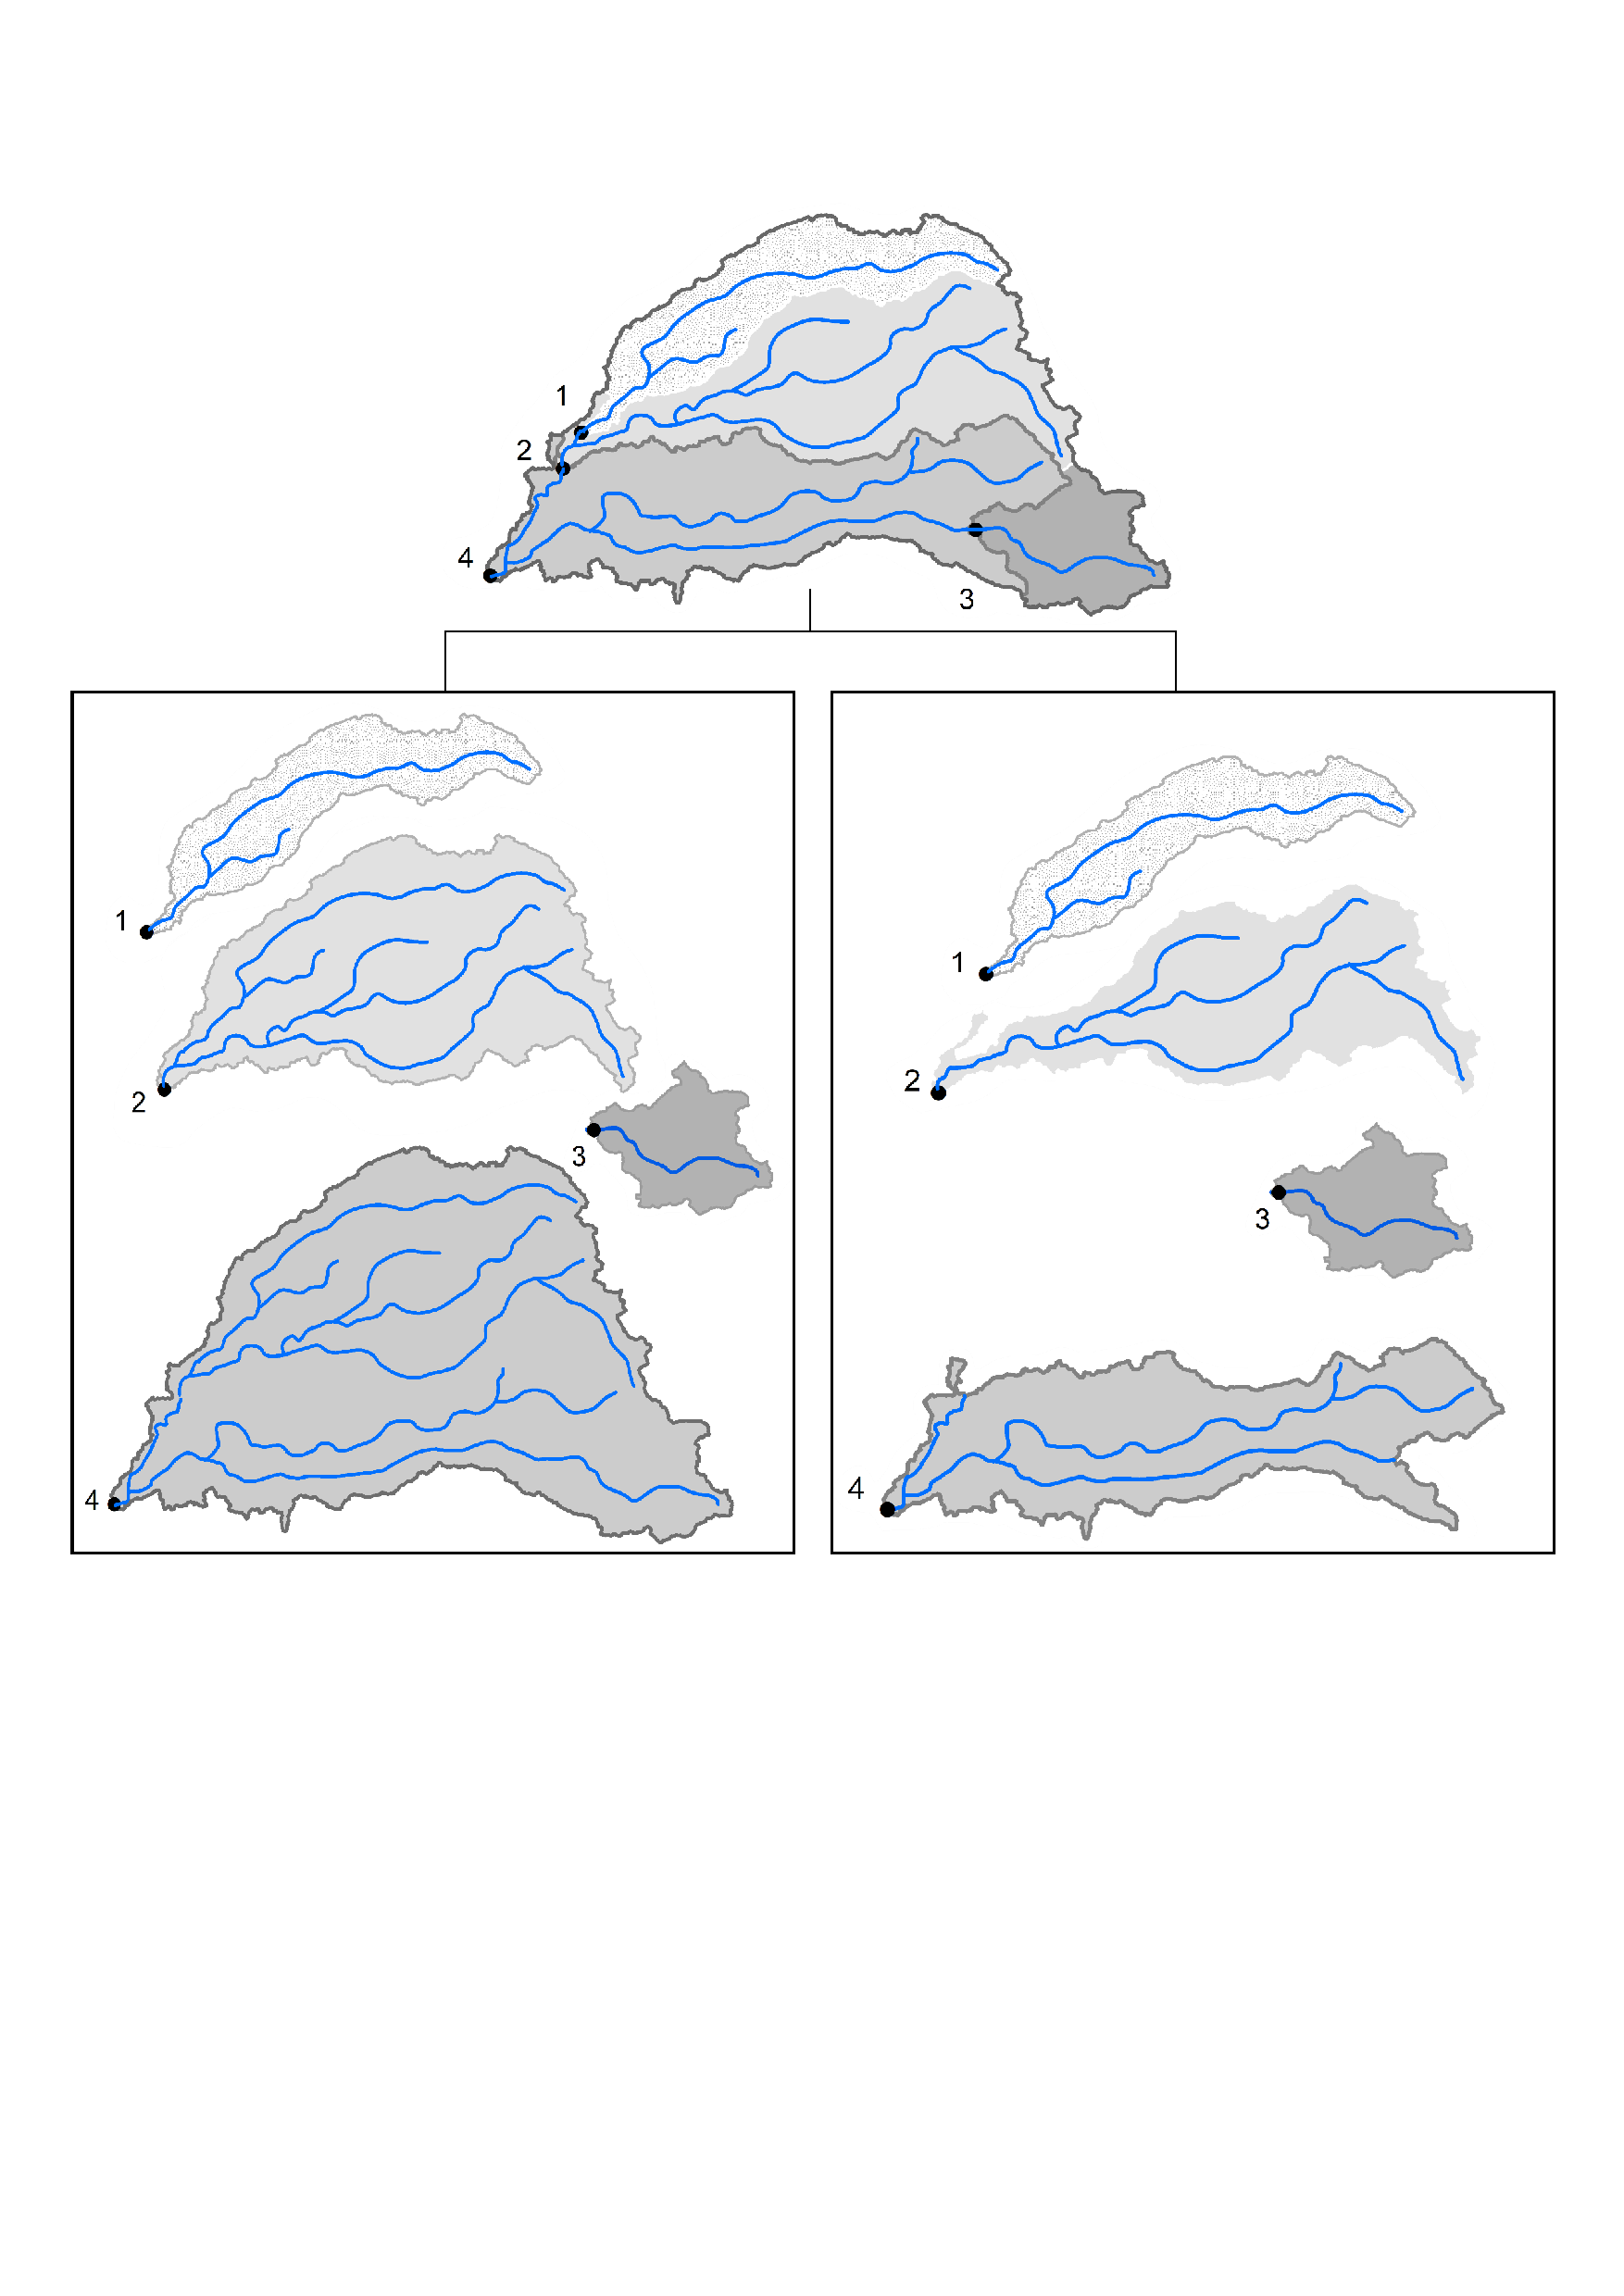
\includegraphics[width=\textwidth, trim={0 29.5cm 0 3.8cm}, clip=true]{plots/agg_and_inc_basins.pdf}
	\end{subfigure}% 
	\hfill
	\begin{subfigure}{.35\textwidth}
  		\centering
 		 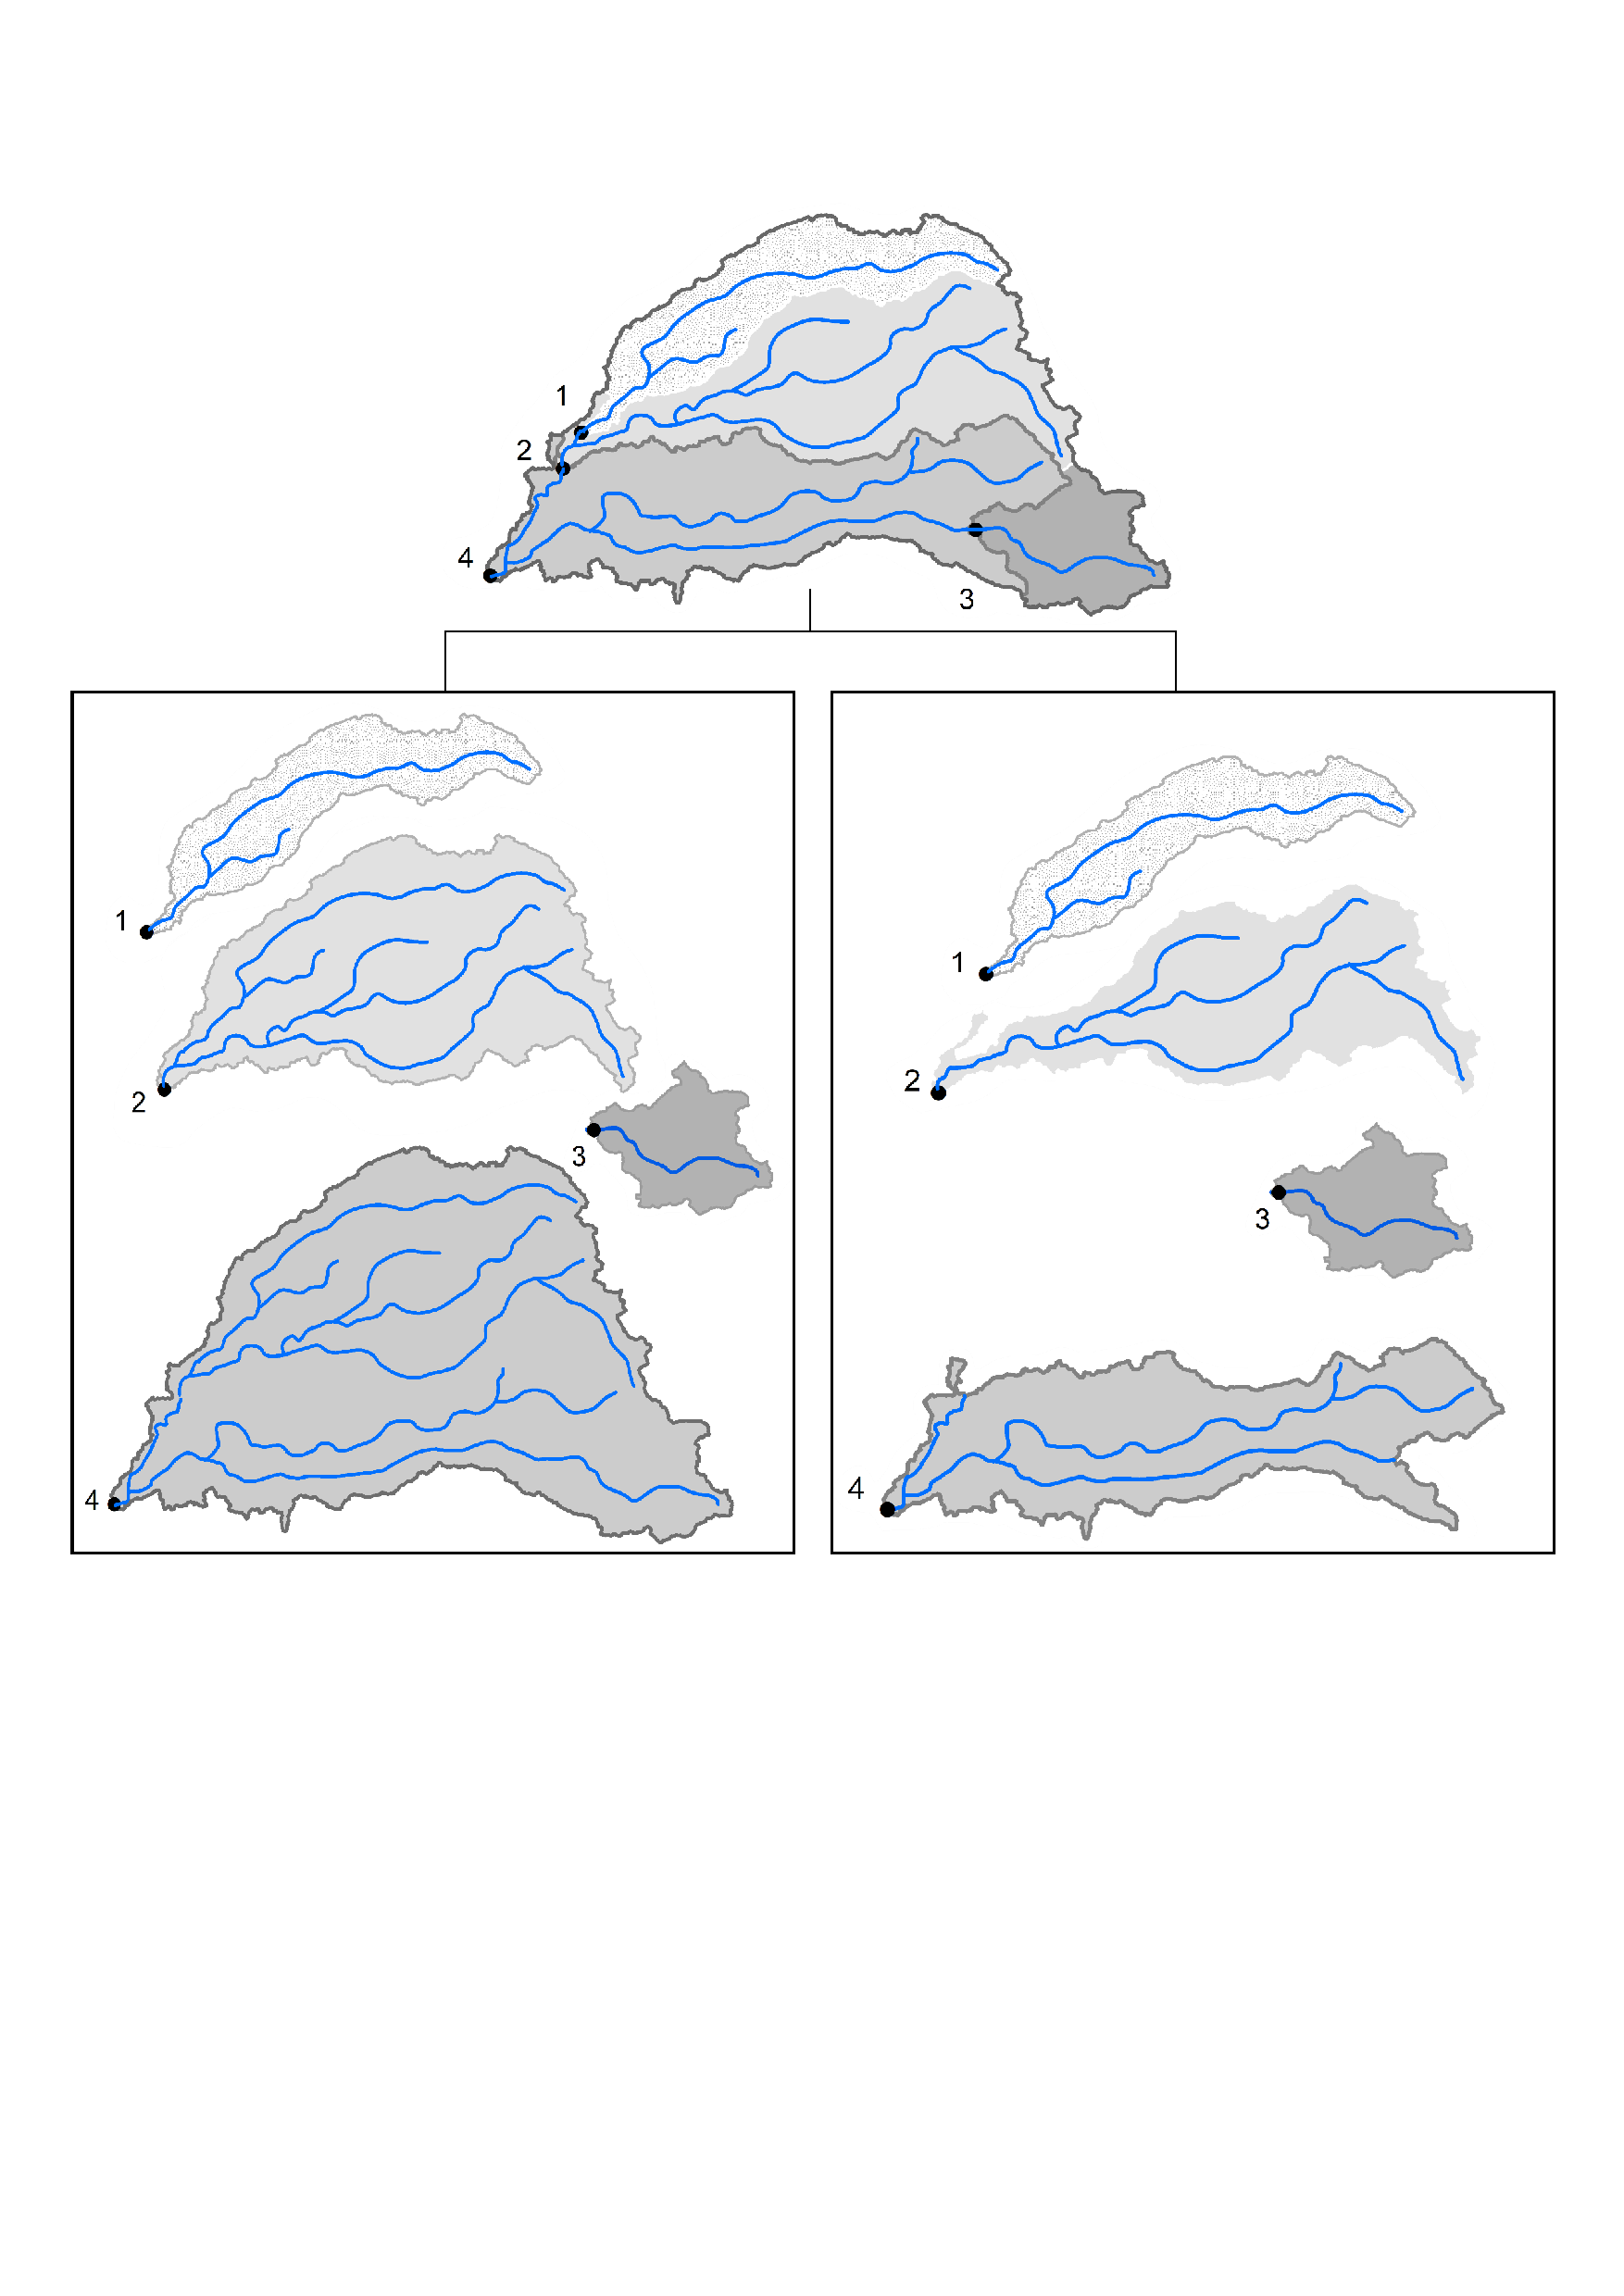
\includegraphics[width=\textwidth, trim={0 13cm 15cm 12.65cm}, clip=true]{plots/agg_and_inc_basins.pdf}
  		\caption{Aggregate Basins}
  		\label{fig:aggbasins}
	\end{subfigure}% 
	\begin{subfigure}{.35\textwidth}
  		\centering
  		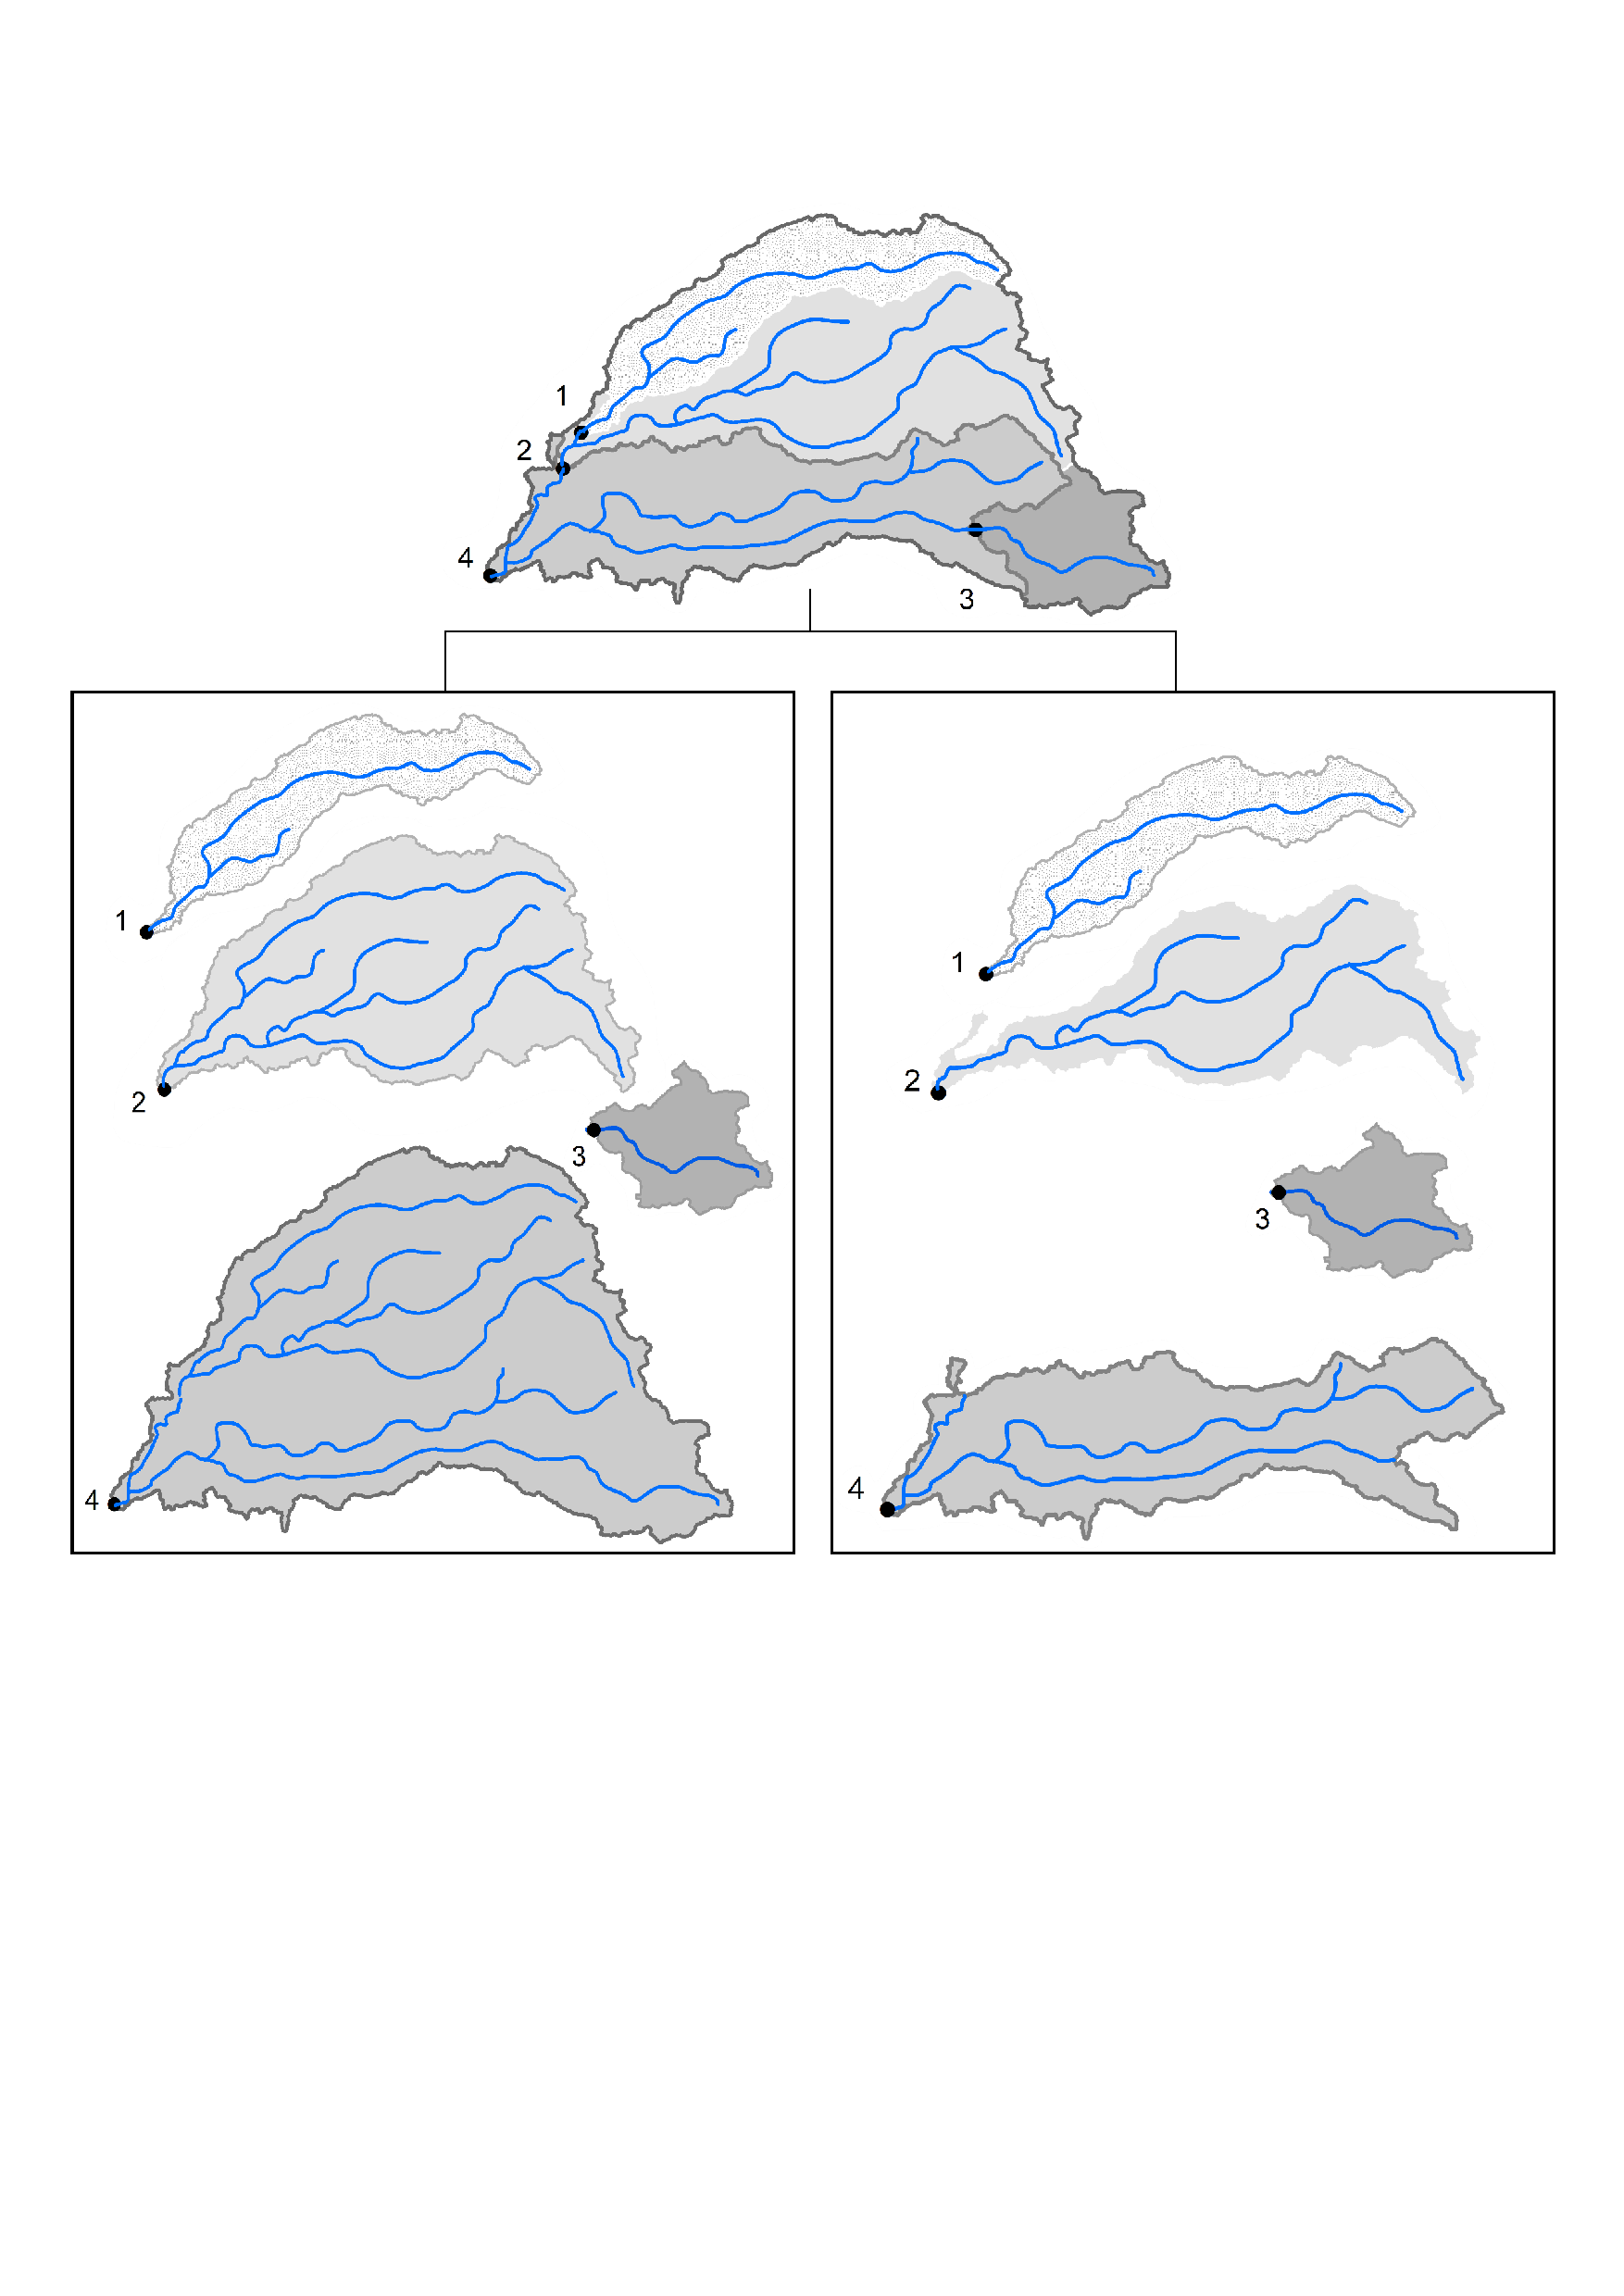
\includegraphics[width=\textwidth, trim={15cm 13cm 0 12.65cm}, clip=true]{plots/agg_and_inc_basins.pdf}
  		\caption{Incremental Basins}
  		\label{fig:incbasins}
	\end{subfigure}
	\caption{A basin's hydrologic response can be interpreted in two fundamentally different ways: (a) aggregate basins, where each basin's response is a function of all the land above the outlet that drains to the outlet, or (b) incremental basins, where each piece of land below an outlet incrementally alters the observed flows from gauges above it.}
	\label{fig:aggincbasins}
\end{figure}

% In addition, the unimpaired flows can be presented in a cumulative form, starting with zero at the beginning of the \textit{water year}. Water years are different from normal calendar years, since part of the precipitation that falls in late fall and winter accumulates as snow and does not drain until the following spring or summer's snowmelt. In California, each year's water year starts on the October of the year before. Hydrologists, sometimes, model and use the cumulative form of precipitation and runoff rather than their non-cumulative values. 

In this chapter, we have two types of data pre-processing: aggregate and incremental basins. Each data transformation method reflects our way of viewing hydrologic processes. Neither is ``right" as they are merely philosophical views of hydrologic processes. 

%----------------------------------------------------------------------------------------------------------------------------------------------------------------------------------------------------------
\section{Methods}
%-----------------------------------------------
\subsection{Model Types and Loss Functions}
The models considered and their parameters are explained below (Table \ref{table:modelspar}).

\begin{table*}[h]\renewcommand{\arraystretch}{1} 
	\linespread{1.0}
	\centering
	\caption{Model types and their parameters.}
	\begin{tabular}{p{1.5cm}p{2.5cm}p{5.5cm}p{5cm}} % must add to 16.5
		\toprule
		Model & R & Parameters defined in  & Parameters selected\\
		type & package & model formulation & through cross validation\\
		\midrule
		LM & stats & not applicable & not applicable\\
		\addlinespace
		GLM & stats & family=Tweedie & var.power=1.1 \\
		& statmod & link.power=0 & \\
		& & maxit=1000 & \\
		\addlinespace
		RF & randomForest & ntree=500 & mtry=20\\
 		&  & sampsize=length(training set) & \\
 		&  & nodesize=5 & \\
		\addlinespace
		NN & keras & batch\_size=25 & epochs=100 \\
 		&  & validation\_split=0.2 & \\
		\bottomrule
	\end{tabular}
	\label{table:modelspar}
\end{table*}

%-----------------------------------------------
\subsubsection*{Linear Multivariate Regression Models}
In 1805, Adrien Marie Legendre introduced the least squares method of estimating parameters as an appendix to his book on the paths of comets. A few years later, Carl Freidrich Gauss also published the method \cite{stigler1981gauss}. The method is brought to perfection with its application to linear regression and curve fitting. 

Linear Multivariate Regression models (LM) are customarily made of systematic and random error components, where the errors are usually assumed to have Normal distribution (Equation \ref{eq:lmdef}). 
\begin{equation} \label{eq:lmdef}
	\begin{aligned}
		& Y \sim N(\mu, \sigma \textsuperscript{2}) \mathrm{: random}  \\
		& \mu=X\beta \mathrm{: systematic}
	\end{aligned}
\end{equation} 

Given the model, the fitted values can be estimated by Equation \ref{eq:fitted}.
\begin{equation} \label{eq:fitted}
	Y^{sim}_i = \beta_{0} +\beta_{1} X_{1i} +\beta_{2} X_{2i} +\cdots +\beta_{i} X_{ki}
\end{equation} 

The unknown parameters in Equation \ref{eq:fitted} are: $\beta_{0}$ (the overall mean) and $\beta_{k}$ (the regression coefficients). To find the best fit, much like simple linear regression, we need to estimate the unknown parameters by minimizing a loss function, customarily the residual sum of squares (RSS) (Equation \ref{eq:rss}).

\begin{equation} \label{eq:rss}
	\begin{split}
		RSS &= \sum^n_{i=1}e^{2}_{i} \\
		&= \sum^n_{i=1}(Y^{obs}_{i} - y^{sim}_i)^2 \\
		&= \sum^n_{i=1}(Y^{obs}_{i}-\beta_{0} +\beta_{1} X_{1i} +\beta_{2} X_{2i} +\cdots +\beta_{i} X_{ki})
	\end{split}
\end{equation} 

The {\tt lm()} function in R constructs LMs. They are easy to understand and interpret, which makes them a great first cut at predictive modeling. However, they over simplify reality (hydrologic processes are not linear) and lack precision (as demonstrated by the goodness-of-fit measures). Another major flaw is that a linear predictor can give predictions that are physically impossible (e.g., negative flows). Here, the variance cannot be considered constant since there is a boundary on the response. These shortcomings can be overcome with generalized linear models. 

%-----------------------------------------------
\subsubsection*{Generalized Linear Regression Models}
In 1972, Nelder and Wedderburn introduced Generalized Linear Regression models \linebreak (GLM). This work allowed for a unified fitting procedure, despite the type of error distribution, based on likelihood \cite{nelder1972generalized}. Therefore, unlike LMs, GLMs can accommodate non-Normal distributions of error. However, except for Normal distributions most other distributions do not have a closed-form solution. 

In GLMs, the linear model is related to the response variable via a link function. This function allows the magnitude of the variance of each measurement to be a function of its predicted value. Therefore a GLMs components are (Equation \ref{eq:glmdef}): 
\begin{equation} \label{eq:glmdef}
	\begin{aligned}
		& Y \sim P(\mu, \phi)  \mathrm{: random}\\
		& g(\mu)=X\beta \mathrm{: systematic}
	\end{aligned}
\end{equation} 

Where P is the distribution of random errors, and $g(\mu)$ is the link function. P and g can be specified by the user.

The {\tt glm()} function in R constructs GLMs. The GLMs developed here are characterized by the \textit{Tweedie distribution}, since the outcome (i.e., unimpaired flow) is continuous, non-negative, skewed, and unbalanced with exact zeros. Tweedie distributions are a special case of exponential dispersion models where the variance function is a power function (Equation \ref{eq:glmvar}), and the link, or the function used to explain how the expectation of the outcome is related to the linear predictor can be specified in terms of Box-Cox transformations \cite{jorgensen1997theory}.
\begin{equation} \label{eq:glmvar}
	var(Y)=V(\mu)\phi=\mu^\alpha \phi
\end{equation}

The power, alpha, can be set by the user, or determined through cross-validation. Special cases include Normal ($\alpha$=0), Poisson ($\alpha$=1), Gamma ($\alpha$=2), and inverse-Gaussian ($\alpha$=3) GLMs . Here, we set the power $\alpha$ to be 1.1. The link $g$ can be specified as log or identity. Here, we used the log link. 

Therefore, the above model assumes that $y_i \sim Tweedie_{\alpha}(\mu_i, \phi)$ where
\begin{equation*}
	var(Y_i)=\mu_i^{1.1} \phi
\end{equation*}
and 
\begin{equation*}
	log(\mu_i)=\beta_{0} +\beta_{1} X_{1i} +\beta_{2} X_{2i} +\cdots +\beta_{i} X_{ki}
\end{equation*}

The regression coefficients, $\beta_{j}$, were estimated by maximum likelihood. The dispersion parameter, $\phi$, was estimated using the residual sum of squared residuals, otherwise called the Pearson estimator.

Both LMs and GLMs are parametric models. For prediction purposes non-parametric methods are proven to perform better since their form is shaped by the data and not fixed a priori. Therefore, next, we consider a non-parametric modeling method, random forests. 

%-----------------------------------------------
\subsubsection*{Tree Building Algorithms} 
Classification and Regression Trees (CARTs) involve stratifying or segmenting the predictor space, into a number of regions, using a series of if-then statements. At each internal node in the tree, a test is made to one of the inputs. Depending on the outcome of the test (or split rule), the algorithm goes to either the left or the right sub-branch of the tree. Eventually the algorithm arrives at a terminal node, which contains a prediction. The prediction for a given observation is the mean or the mode of the training observations in the region to which it belongs \cite{breiman1984classification}. 

 In essence, each tree is a series of split rules. The split rule is found using a greedy top-down search for recursively splitting of the data into binary partitions. It is greedy, because, the split rule at each internal node is selected to maximize the homogeneity of its child nodes, without consideration of nodes further down the tree, yielding only locally optimal trees \cite{grubinger2011evtree}. For regression trees, the mean of all the observation points that fall within a branch is considered the prediction of that branch in the tree. The best tree is one which has the minimum test error rate calculated by the RSS. 

Since trees have a finite number of terminal nodes (CARTs are pruned based on a complexity parameter, $\alpha$), the prediction of these methods are discrete, and therefore, not particularly suited to modeling a continuous variable. In addition, CARTs suffer from high variance; trees grown on different subsets of the training set will produce different predictions. This phenomenon is one of the major drawbacks of CARTs. Methods such as \textit{bagging} \cite{breiman1996bagging}, \textit{random forests} \cite{breiman2001random}, \textit{boosting} \cite{friedman2001greedy} and \textit{bumping} \cite{grubinger2010regression} attempt to improve the prediction accuracy of trees with the idea that combining and averaging trees reduces variance. 

A Random Forest (RF) consists of an assemblage of unpruned CART models. Each CART model in an RF is different because it is grown using: (1) a new training set: in each bootstrapped training set, about one-third of the instances are left out; and (2) random feature selection: each time a split in a tree is considered, a random sample of predictors is chosen as split candidates from the full set of predictors. This process de-correlates the trees. 
%Suppose there is one very strong predictor in the dataset, along with other moderately strong predictors. Then, in the collection of trees, most or all trees will use this strong predictor in the top split. Consequently, all trees will look quite similar. So, the predictions from the trees will be highly correlated. However, by forcing each split to consider only a subset of the predictors makes the resulting trees less variable and more reliable \cite{james2013introduction}. 
This strategy, using a random selection of features to split each node, introduces some randomness that improves the accuracy of the predictions of the trees as a whole and yields error rates that are robust with respect to noise \cite{breiman2001random}.

%\begin{equation} \label{eq:rfdef}
%	\hat {y} = {\frac {1}{m}}\sum _{j=1}^{m}\sum _{i=1}^{n}W_{j}(x_{i},x')\,y_{i}=\sum _{i=1}^{n}\left({\frac {1}{m}}\sum _{j=1}^{m}W_{j}(x_{i},x')\right)\,y_{i}
%\end{equation}
%
%Equation \ref{eq:rfdef} shows that the RF is essentially a weighted neighborhood scheme, with weights that average of the individual trees.

The {\tt randomForest()} function in the {\tt randomForest} library \cite{liaw2002classification}, constructs RF models. This function takes in tuning parameters such as mtry, ntree, sampsize, and maxnodes:

{\tt mtry}: In RFs, internal estimates monitor error, strength and correlation, which are used to show the response to increasing the number of features used in the splitting. Here, this parameter was set to 20 out of the full 25 predictor variables available found through cross-validation.

{\tt ntree}: The generalization error of a forest of trees depends on the strength of the individual trees in the forest and the correlation between them \cite{breiman2001random}. This error converges to a limit as the number of trees in the forest increases. Here, the number of trees was set to the default 500. 

{\tt sampsize}: In RFs, the trees are built on a bootstrap sample of the training data, a sample equal in size to the original dataset, but selected with replacement. Therefore, some observations are not selected, and others are selected more than once. Here, the sample size is set to the default value, the length of the training set.

{\tt maxnodes}: Using the maximum number of terminal nodes, the user can ``prune'' the trees back to a smaller version of itself. Here, we used the default value, which is a function of {\tt nodesize} or the allowed minimum number of observations in each node. The default value for nodesize is 5.   

% These parameters can be fixed by the user or optimized. The benefit of optimizing the parameters become evident when overfitting is concerned \cite{breiman2001random}. Figure \ref{fig:optsettings} shows that, with the exception of mtry, the optimal parameters are the default parameters for this study. 

Like LMs, RFs also typically use the RSS loss function to find the optimal split value. For more information about loss functions see Chapter \ref{ch3:loss}.

% In conclusion, the choice of a suitable model relies on striking the desired balance between three model properties: generality, reality, and precision. Therefore, model selection shouldn't solely rely on statistics; some models better reflect physical foundations in hydrology, and conceptual considerations need to include the desired level of trade-off between optimizing accuracy versus optimizing generality \cite{guisan2000predictive}. Unfortunately, no guide to empirical model selection exists in hydrology. 

%-----------------------------------------------
\subsubsection*{Neural Networks} 
In 1951, Marvin Minsky and graduate student Dean Edmonds built the first neural network (NN) machine. This machine was a randomly connected network of capacitors that have a finite amount of memory and time to keep or remember that memory. The memory holds the probability that a signal will come in one input and another signal will come out of the output. This machine, modeled after the Hebbian theory of learning in the human brain, was one of the first pioneering attempts at artificial intelligence. Shortly after, in 1957, Frank Rosenblatt invents the perceptron, the first \textbf{neural network} for computers. 

[INSERT neural network graph, equation, chain rule for finding optimal parameters, insert discussion on model variables and their specifications] 

%-----------------------------------------------
\subsection{Test Error Approximation}
Blocking cross-validation is used to approximate the test set error. Here, all data for the basin to be modeled is left out of the training data and becomes the test set (i.e., leave one group out cross validation). Therefore, the training data is the data from all the other basins. This process was repeated for all basins in the study, and so, for model evaluation, one LM, GLM, RF, and NN model exists for each basin. For more information about resampling methods see Chapter \ref{ch4:resampling}.

With the developed model's predictions and the observations in the test set, we can calculate the desired model goodness-of-fit: Bias-Corrected Coefficient of Determination (bR\textsuperscript{2}) and Nash-Sutcliffe Efficiency factor (NSE) (Equations \ref{eq2:r2}, \ref{eq2:br2}, and  \ref{eq2:nse}). See appendix \ref{d:mof} for more model measures-of-fit.

\begin{equation} \label{eq2:r2}
	R^{2} = \ \left(\frac{\sum^n_{i=1}{\left(Y^{obs}_i-\overline{Y^{obs}}\right)\left(Y^{sim}_i-\overline{Y^{sim}}\right)}}{\sqrt{\sum^n_{i=1}{\left(Y^{obs}_i-\overline{Y^{obs}}\right)^2}}\sqrt{\sum^n_{i=1}{\left(Y^{sim}_i-\overline{Y^{sim}}\right)^2}}}\right)^2  \quad R^{2} \in [0,1] \\
\end{equation}

$R^2$ is insensitive to additive and proportional difference between model simulation and observations. One can simply show that for a non zero value of $\beta_0$ and $\beta_1$, if the predictions follow a linear form, $Y^{sim}=\beta_0 + \beta_1 Y^{obs}$, the $R^2$ equals one \cite{legates1999evaluating}. Therefore, for a proper model assessment, it is recommended that the slope of the predicted vs. observed graph be reported or systematically included as in Equation \ref{eq2:br2}. 

\begin{equation} \label{eq2:br2}   
	bR^{2} =  
	\begin{cases}
		\text{$\abs{b}R^2$} & \quad\text{for b}\le1\\
		\text{$\abs{b}^{-1}R^2$} &\quad\text{for b}>1  \quad bR^{2} \in [0,1] \\
	\end{cases}
\end{equation}

By weighting $R^2$, under and over predictions are quantified together with the model dynamics which results in a more comprehensive reflection of model results.

Another commonly used model goodness-of-fit is the the Nash-Sutcliffe efficiency factor (Equation \ref{eq:nse}). 

\begin{equation} \label{eq2:nse}
	NSE =\ 1-\frac{\sum^n_{i=1}{{\left(Y^{sim}_i-Y^{obs}_i\right)}^2\ }}{\sum^n_{i=1}{{\left(Y^{obs}_i-\overline{Y^{obs}}\right)}^2\ }} \quad NSE \in (-\infty,1] 
\end{equation}

A Nash-Sutcliffe efficiency factor of lower than zero indicates that the mean value of the observed time series would have been a better predictor than the model. Like the bR\textsuperscript{2}, the largest disadvantage of the Nash-Sutcliffe efficiency factor is the fact that the differences between the observed and predicted values are calculated as squared values. As a result, larger values in a time series are strongly overestimated whereas lower values are neglected \cite{legates1999evaluating}. For the quantification of runoff predictions this leads to an overestimation of the model performance during peak flows and an underestimation during low flow conditions \cite{krause2005comparison}.

%-----------------------------------------------
\subsection{Post-Processing}
In post-processing all model predictions are modified so as to be comparable to original gauge flows; all cumulative values are back-transformed into non-cumulative forms, and all incremental basins are back-transformed into aggregate forms. In other words, the steps used in pre-processing are reversed so as to fairly compare the goodness-of-fit across all models.

%------------------------------------------------------------------------------------------------------------------------------------------------------------------------
\section{Results}

%-----------------------------------------------
\subsection{Model Evaluation}
Figure \ref{fig:obsvpred} shows the predicted unimpaired flows versus the observed for each model type in order of increasing NSE. A perfect model will follow the $y=x$ line. The regression line shows a tendency for the LM and RF aggregate and incremental models to under predict and for the GLM aggregate and incremental models to slightly over predict the unimpaired flows. Under predicting flows are generally bad in times of floods and over predicting flows are generally bad in times of droughts, since both lead to decisions that are both inaccurate and not conservative. The NN outperforms other models and it is somewhat insensitive to the input data pre-processing.

% Squared error loss functions tend to predict large values at the expense of smaller ones, since larger errors have more of a penalty (i.e., are being squared). Hence, the models failure at modeling basins at a low hierarchy compared to higher hierarchies. This phenomenon will be explored in other chapters. 

%\begin{figure}
%	\centering
%	\begin{subfigure}{.5\textwidth}
%  		\centering
% 		 \includegraphics[width=\textwidth, trim={0 0 0 0}, clip=true]{plots/rplot27_obsvspred2_lm_agg.png}
%  		\caption{LM Aggregate}
%  		\label{fig:lmagg}
%	\end{subfigure}% 
%	\begin{subfigure}{.5\textwidth}
%  		\centering
% 		 \includegraphics[width=\textwidth, trim={0 0 0 0}, clip=true]{plots/rplot27_obsvspred2_lm_inc.png}
%  		\caption{LM Incremental}
%  		\label{fig:lminc}
%	\end{subfigure}% 
%	\hfill
%	\begin{subfigure}{.5\textwidth}
%  		\centering
% 		 \includegraphics[width=\textwidth, trim={0 0 0 0}, clip=true]{plots/rplot27_obsvspred2_glm_agg.png}
%  		\caption{GLM Aggregate}
%  		\label{fig:glmagg}
%	\end{subfigure}% 
%	\begin{subfigure}{.5\textwidth}
%  		\centering
% 		 \includegraphics[width=\textwidth, trim={0 0 0 0}, clip=true]{plots/rplot27_obsvspred2_glm_inc.png}
%  		\caption{GLM Incremental}
%  		\label{fig:glminc}
%	\end{subfigure}% 
%	\hfill
%	\begin{subfigure}{.5\textwidth}
%  		\centering
% 		 \includegraphics[width=\textwidth, trim={0 0 0 0}, clip=true]{plots/rplot27_obsvspred2_rf_agg.png}
%  		\caption{RF Aggregate}
%  		\label{fig:rfagg}
%	\end{subfigure}% 
%	\begin{subfigure}{.5\textwidth}
%  		\centering
% 		 \includegraphics[width=\textwidth, trim={0 0 0 0}, clip=true]{plots/rplot27_obsvspred2_rf_inc.png}
%  		\caption{RF Incremental}
%  		\label{fig:rfinc}
%	\end{subfigure}% 
%	\hfill
%	\begin{subfigure}{.5\textwidth}
%  		\centering
% 		 \includegraphics[width=\textwidth, trim={0 0 0 0}, clip=true]{plots/rplot27_obsvspred2_nn_agg.png}
%  		\caption{NN Aggregate}
%  		\label{fig:nnagg}
%	\end{subfigure}% 
%	\begin{subfigure}{.5\textwidth}
%  		\centering
% 		 \includegraphics[width=\textwidth, trim={0 0 0 0}, clip=true]{plots/rplot27_obsvspred2_nn_inc.png}
%  		\caption{NN Incremental}
%  		\label{fig:nninc}
%	\end{subfigure}% 
%	\hfill
%	\caption{The models trained on the four types of data (i.e., aggregate, incremental, cumulative aggregate, and cumulative incremental). The LM generally underpredict unimpaired flows and show a bad fit. The GLMs slightly overpredict unimpaired flows, but show a better fit. The RF generally overpredict unimpaired flows. The RFs, non-parametric models, are a big improvement compared to the linear models, parametric models. Lastly, the NNs, out perform all models.}
%	\label{fig:obsvpred}
%\end{figure}

\begin{figure}
  	\centering
 	\includegraphics[width=\textwidth, trim={0 0 0 0}, clip=true]{plots/rplot27_obsvspred_all.png}
	\caption{The models trained on the four types of data (i.e., aggregate, incremental, cumulative aggregate, and cumulative incremental). The LM generally under predict unimpaired flows and show a bad fit. The GLMs slightly over predict unimpaired flows, but show a better fit. The RF generally over predict unimpaired flows. The RFs, non-parametric models, are a big improvement compared to the linear models, parametric models. Lastly, the NNs, out perform all models.}
	\label{fig:obsvpred}
\end{figure}

Figure \ref{fig:gof} shows how each model scores as to the bR\textsuperscript{2} and NSE. In the LM and GLM the incremental modeling method performs better than the aggregate. In the RF and NN their performances are very similar.

\begin{figure}
	\centering
	\begin{subfigure}{\textwidth}
  		\centering
 		 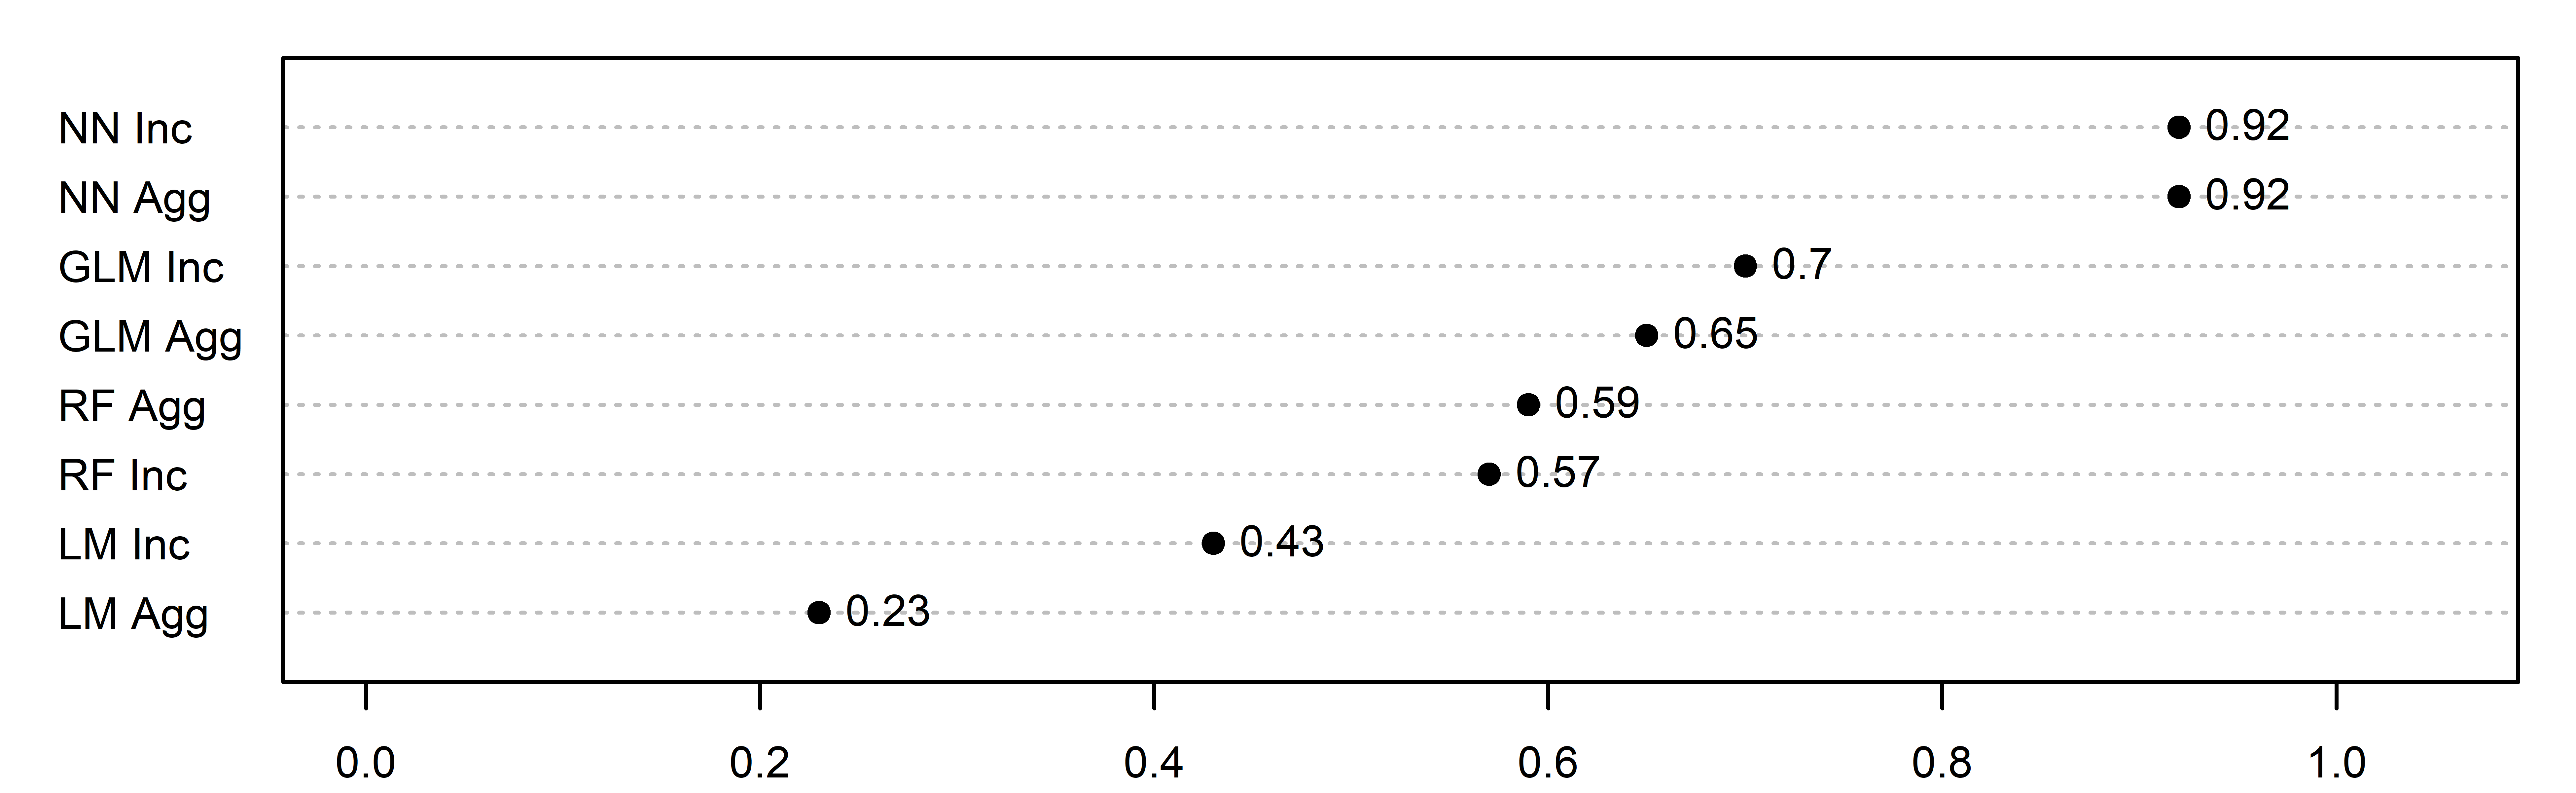
\includegraphics[width=\textwidth, trim={0 0 0 0}, clip=true]{plots/rplot26_gof_bR2.png}
  		\caption{bR\textsuperscript{2}}
  		\label{fig:rmse}
	\end{subfigure}%
	\hfill
	\begin{subfigure}{\textwidth}
  		\centering
  		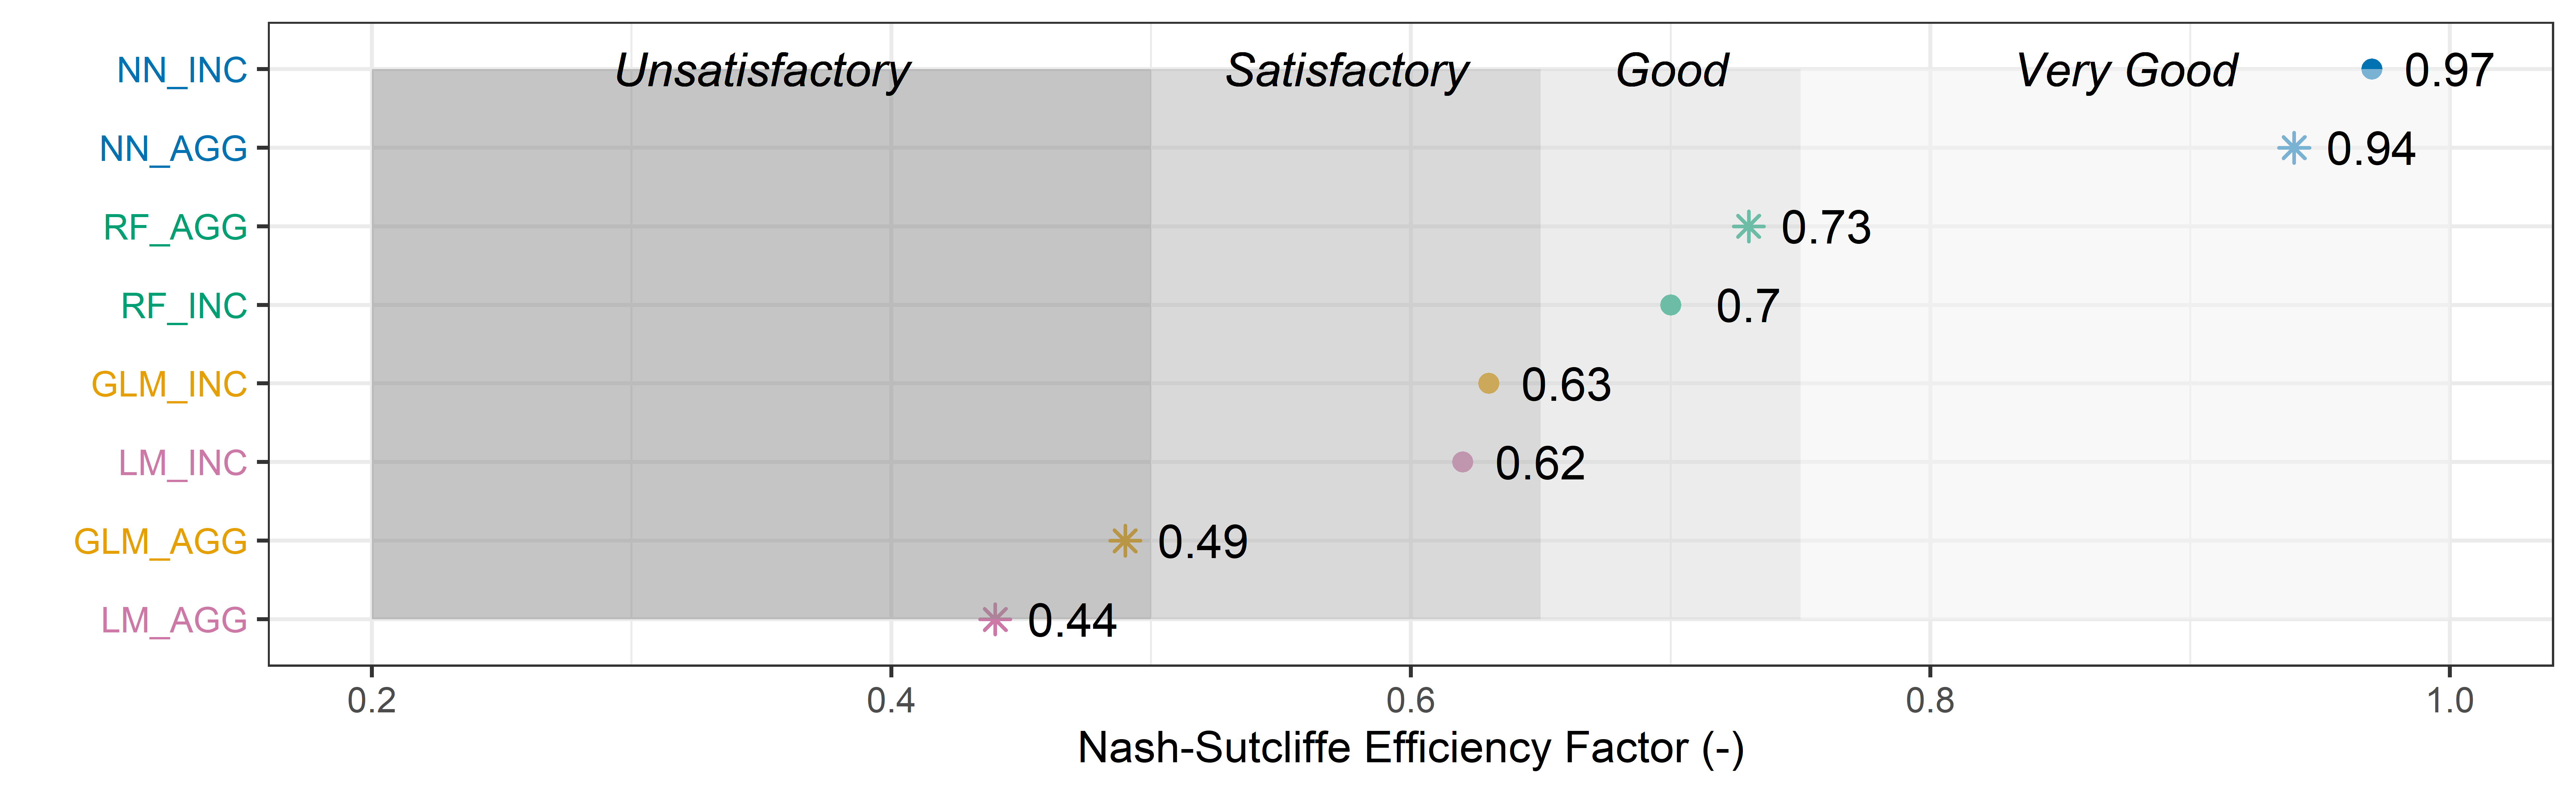
\includegraphics[width=\textwidth, trim={0 0 0 0}, clip=true]{plots/rplot26_gof_NSE.png}
  		\caption{NSE}
  		\label{fig:nse}
	\end{subfigure}
	\caption{The goodness-of-fit of models trained on the two types of data (i.e., aggregate and incremental) as measured by the Coefficient-of-Determination (bR\textsuperscript{2}) and Nash-Sutcliffe Efficiency (NSE). The NN aggregate and incremental model provides the best model performance in the bR\textsuperscript{2} and NSE respectively.}
	\label{fig:gof}
\end{figure}

Figure \ref{fig:resovertime} shows that the models all decrease in accuracy over time. We can hypothesize that this is due to climate change imposing non-stationarity on the hydrologic process. This is further discussed in chapter \ref{ch5:climatechange}.

\begin{figure}
	\centering
	\begin{subfigure}{.5\textwidth}
  		\centering
 		 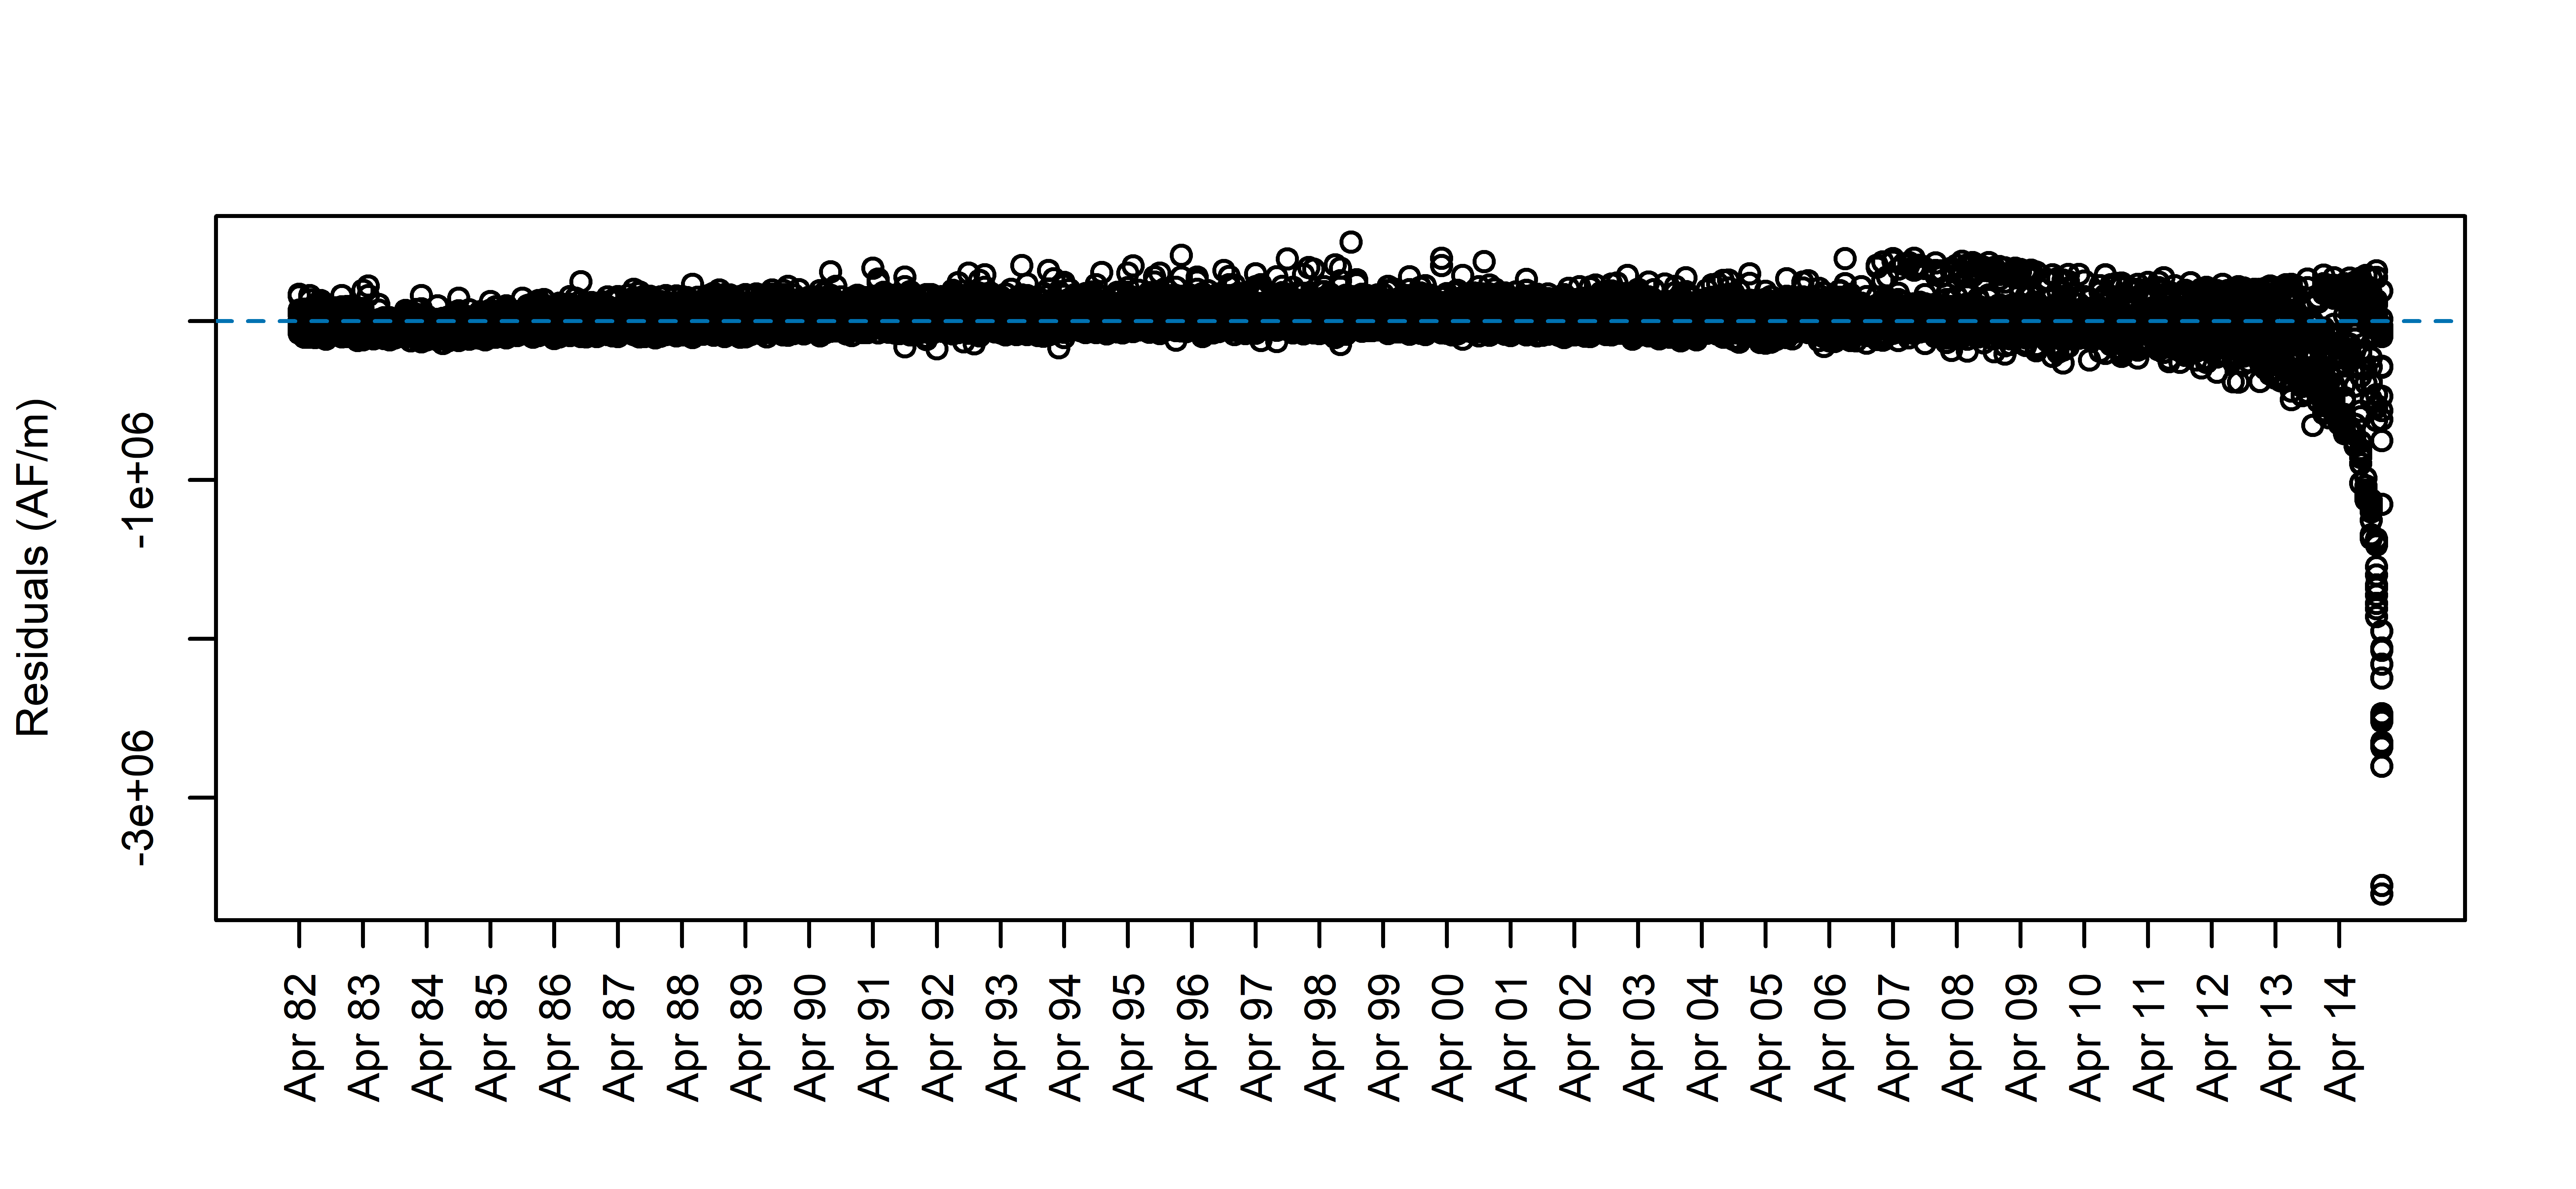
\includegraphics[width=\textwidth, trim={0 0 0 1cm}, clip=true]{plots/rplot22_lmlogo_residovertime_inc.png}
  		\caption{LM Incremental}
  		\label{fig:restimelm}
	\end{subfigure}% 
	\begin{subfigure}{.5\textwidth}
  		\centering
 		 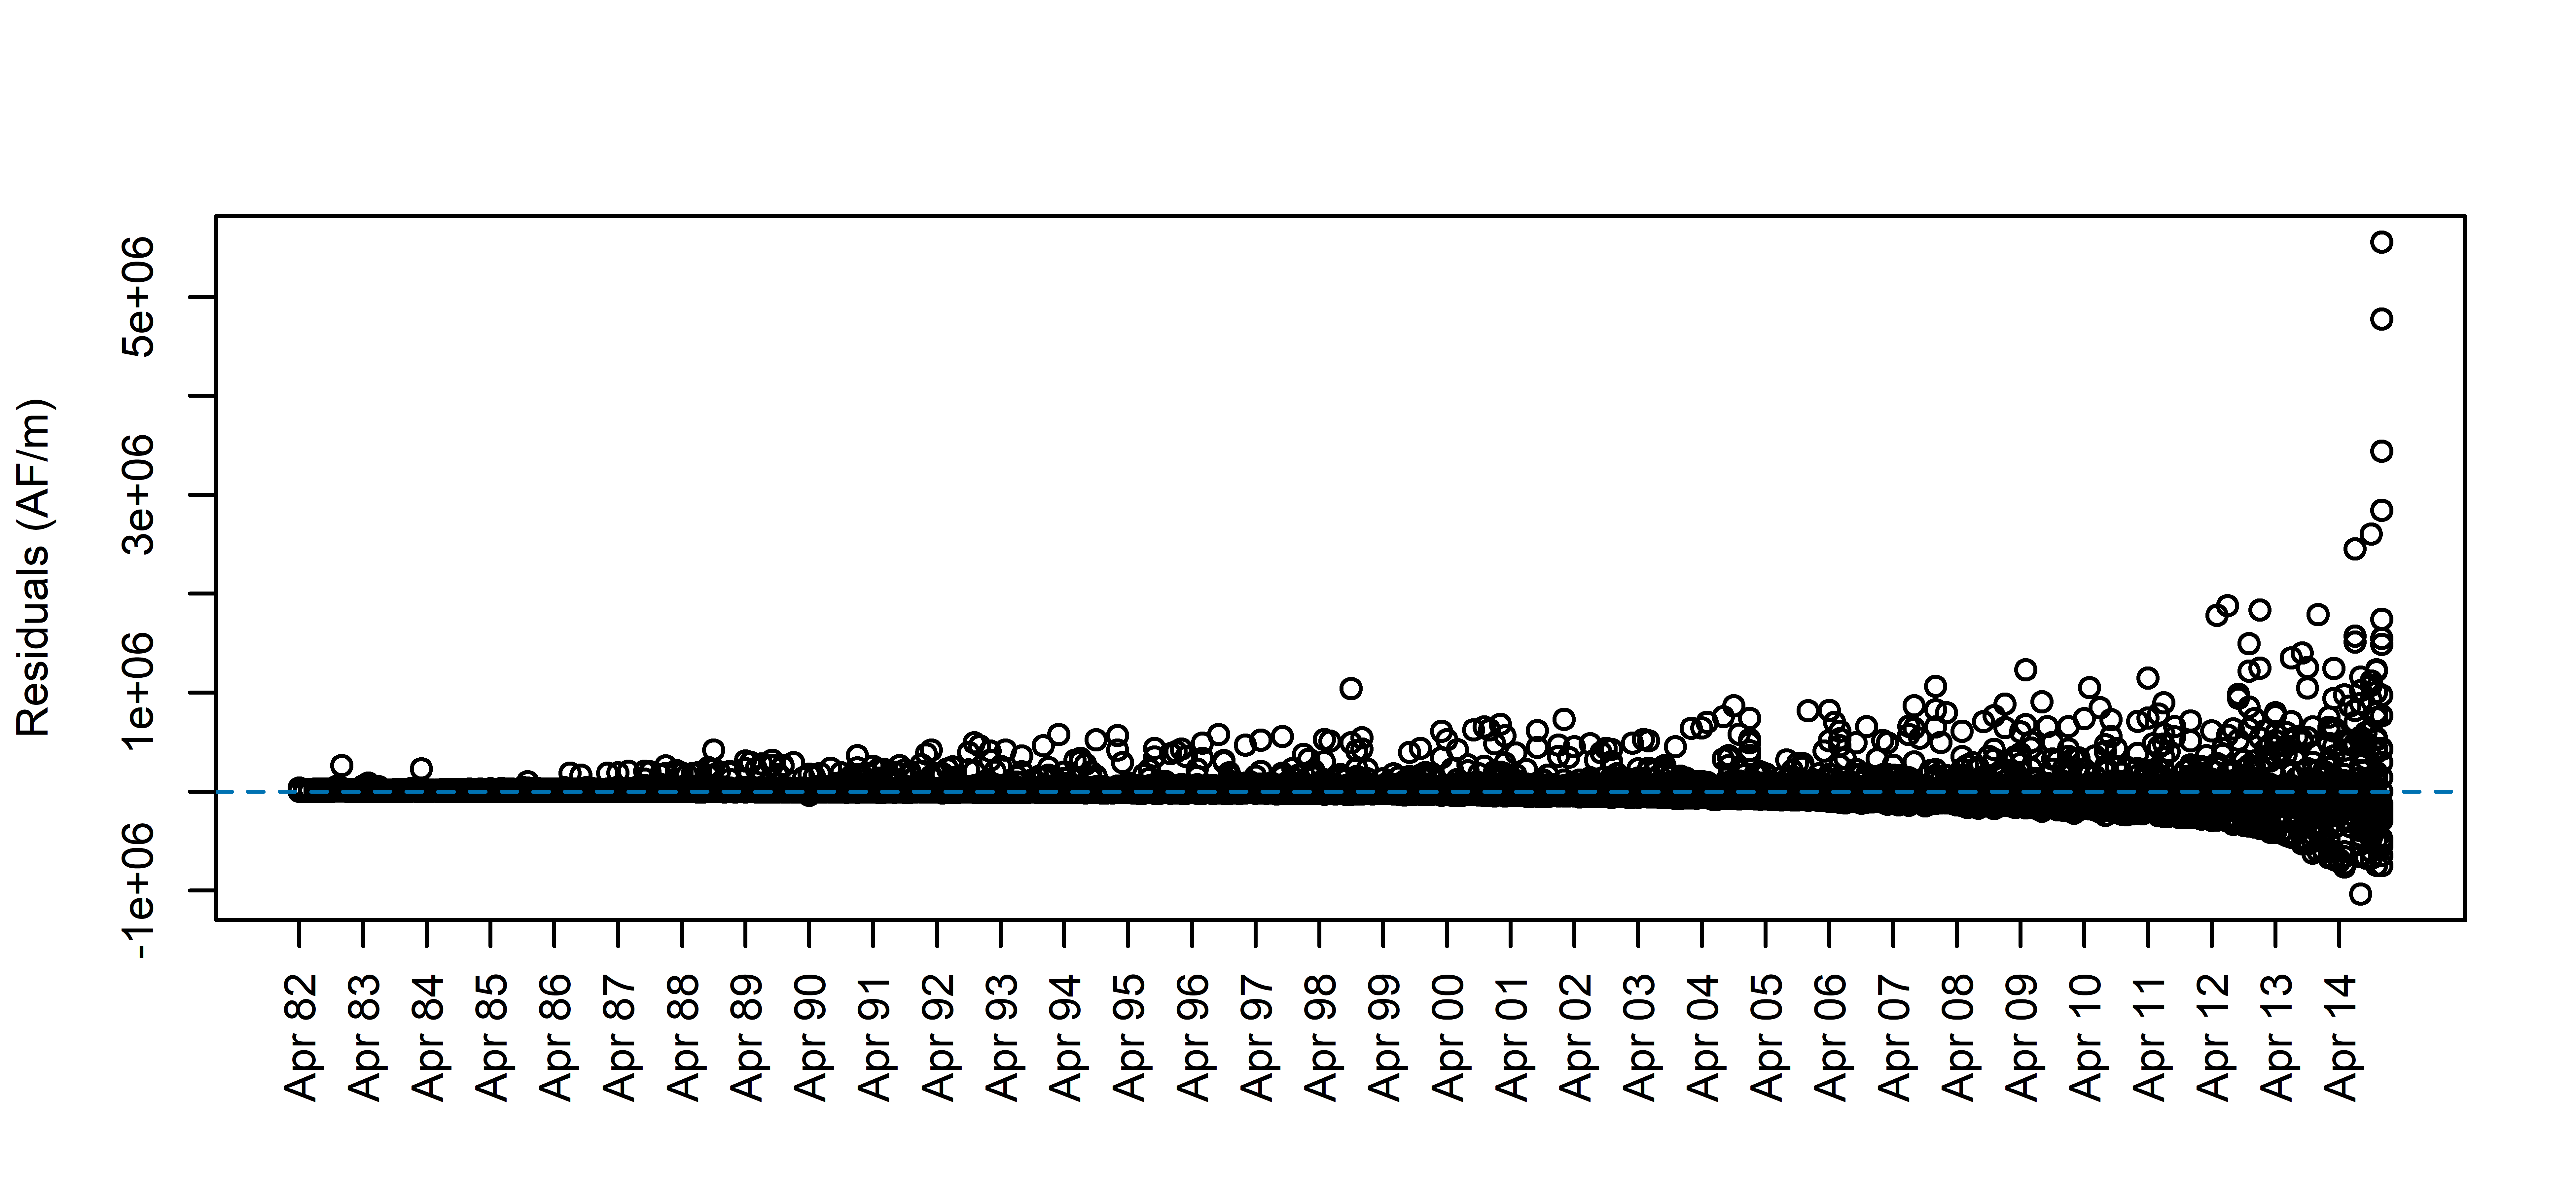
\includegraphics[width=\textwidth, trim={0 0 0 1cm}, clip=true]{plots/rplot22_glmlogo_residovertime_inc.png}
  		\caption{GLM Incremental}
  		\label{fig:restimeglm}
	\end{subfigure}% 
	\hfill
	\begin{subfigure}{.5\textwidth}
  		\centering
 		 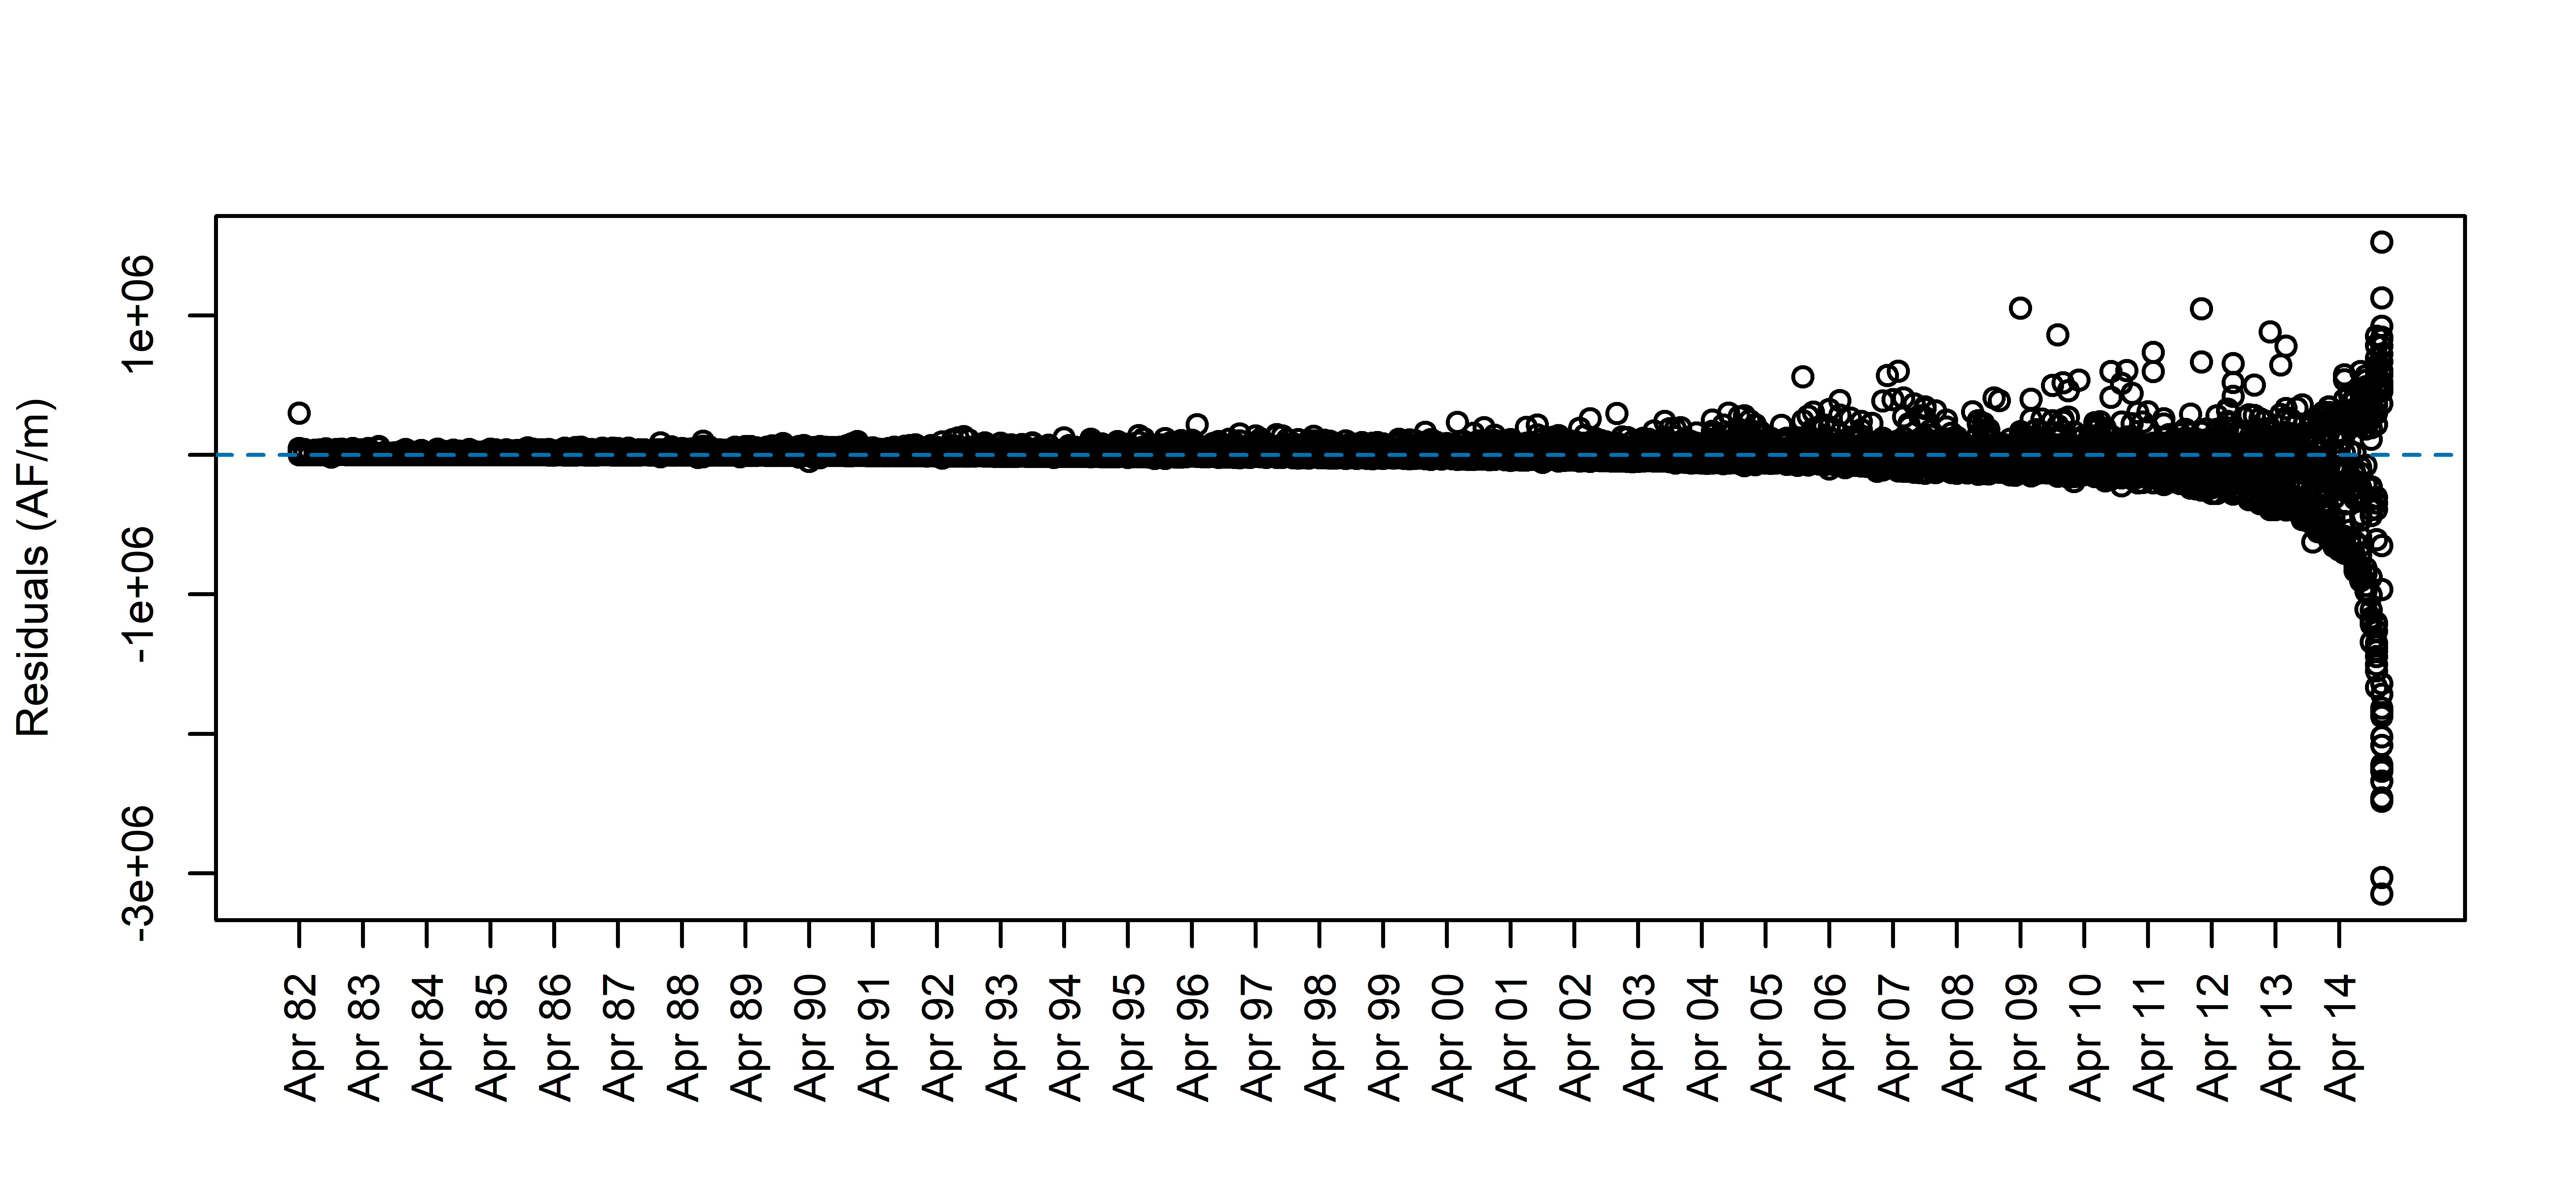
\includegraphics[width=\textwidth, trim={0 0 0 1cm}, clip=true]{plots/rplot22_rflogo_residovertime_inc.png}
  		\caption{RF Incremental}
  		\label{fig:restimerf}
	\end{subfigure}% 
	\begin{subfigure}{.5\textwidth}
  		\centering
  		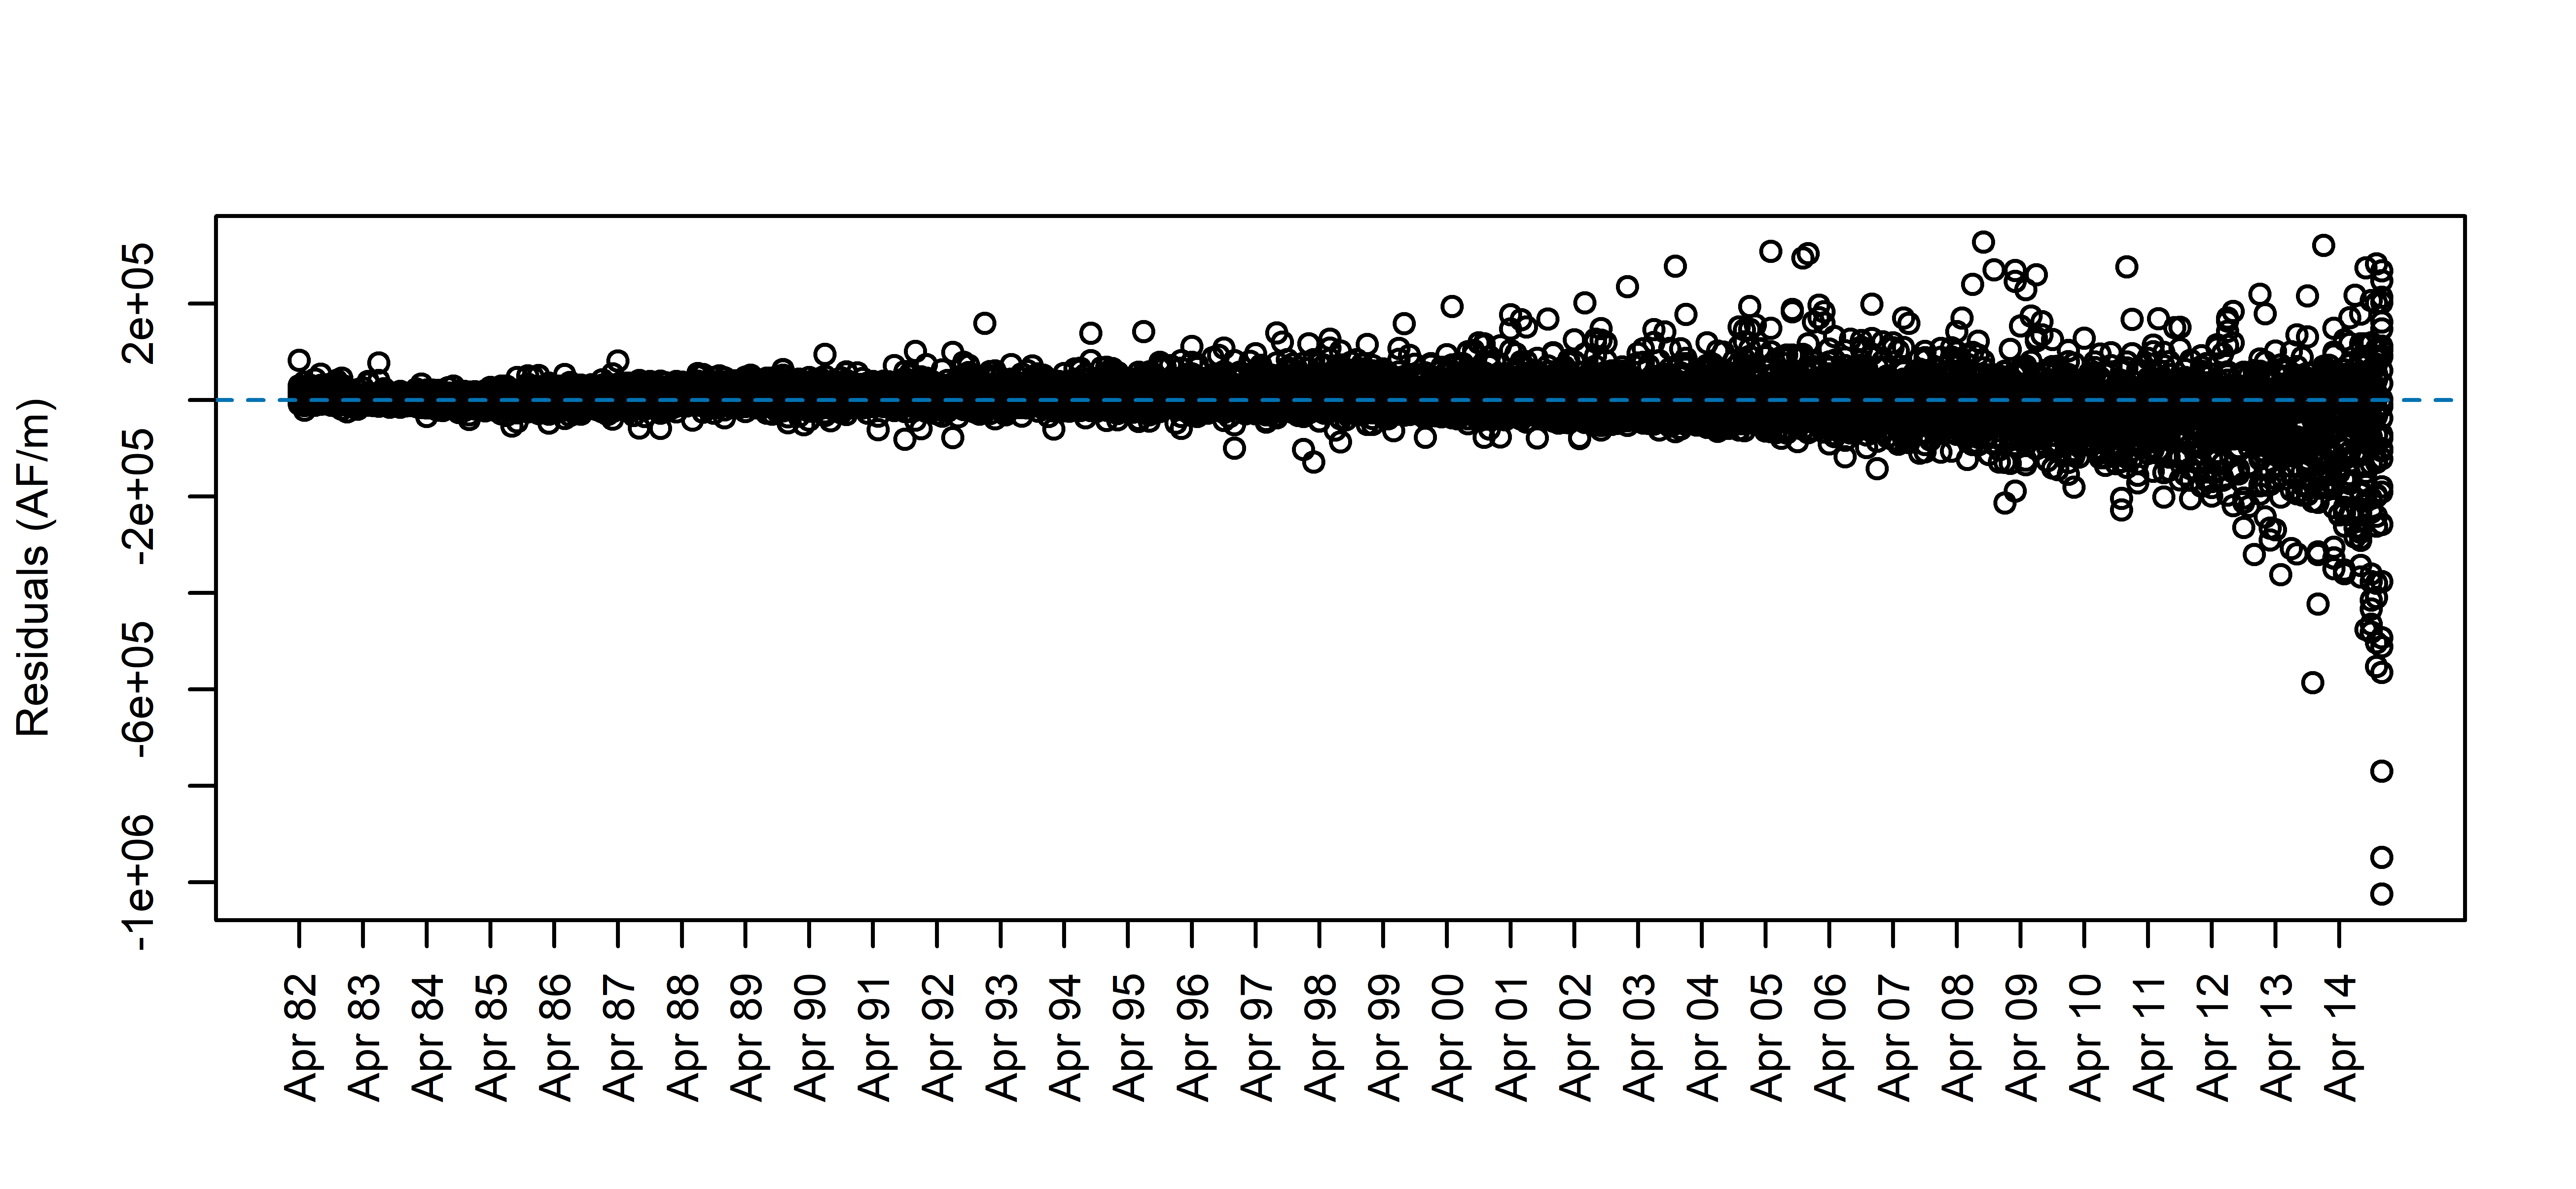
\includegraphics[width=\textwidth, trim={0 0 0 1cm}, clip=true]{plots/rplot22_nnlogo_residovertime_inc.png}
  		\caption{NN Incremental}
  		\label{fig:restimenn}
	\end{subfigure}
	\caption{}
	\label{fig:resovertime}
\end{figure}

In the NSE, the NN incremental model provides the best model performance, therefore, we will now abandon the comparative analysis and examine the spatial distribution of this model.
%-----------------------------------------------
\subsection{Spatial Distribution of Errors}
Figures \ref{fig:incbr2plus} and \ref{fig:aggincbr2comp} show the bR\textsuperscript{2} values for the 67 basins in this study. As expected, the model's ability to predict unimpaired flow varies across California. The model performs better at basins  lower in the network (i.e., have a higher hierarchy). This could be due to: (1) the basins with higher hierarchies generally have larger flows and the model is trained with a squared error loss that penalizes large errors more harshly; or (2) there was substantial value in having flow information upstream (i.e, the decline is error is due to having incremental basins). 

\begin{figure}
	\centering
	\begin{subfigure}{.5\textwidth}
  		\centering
 		 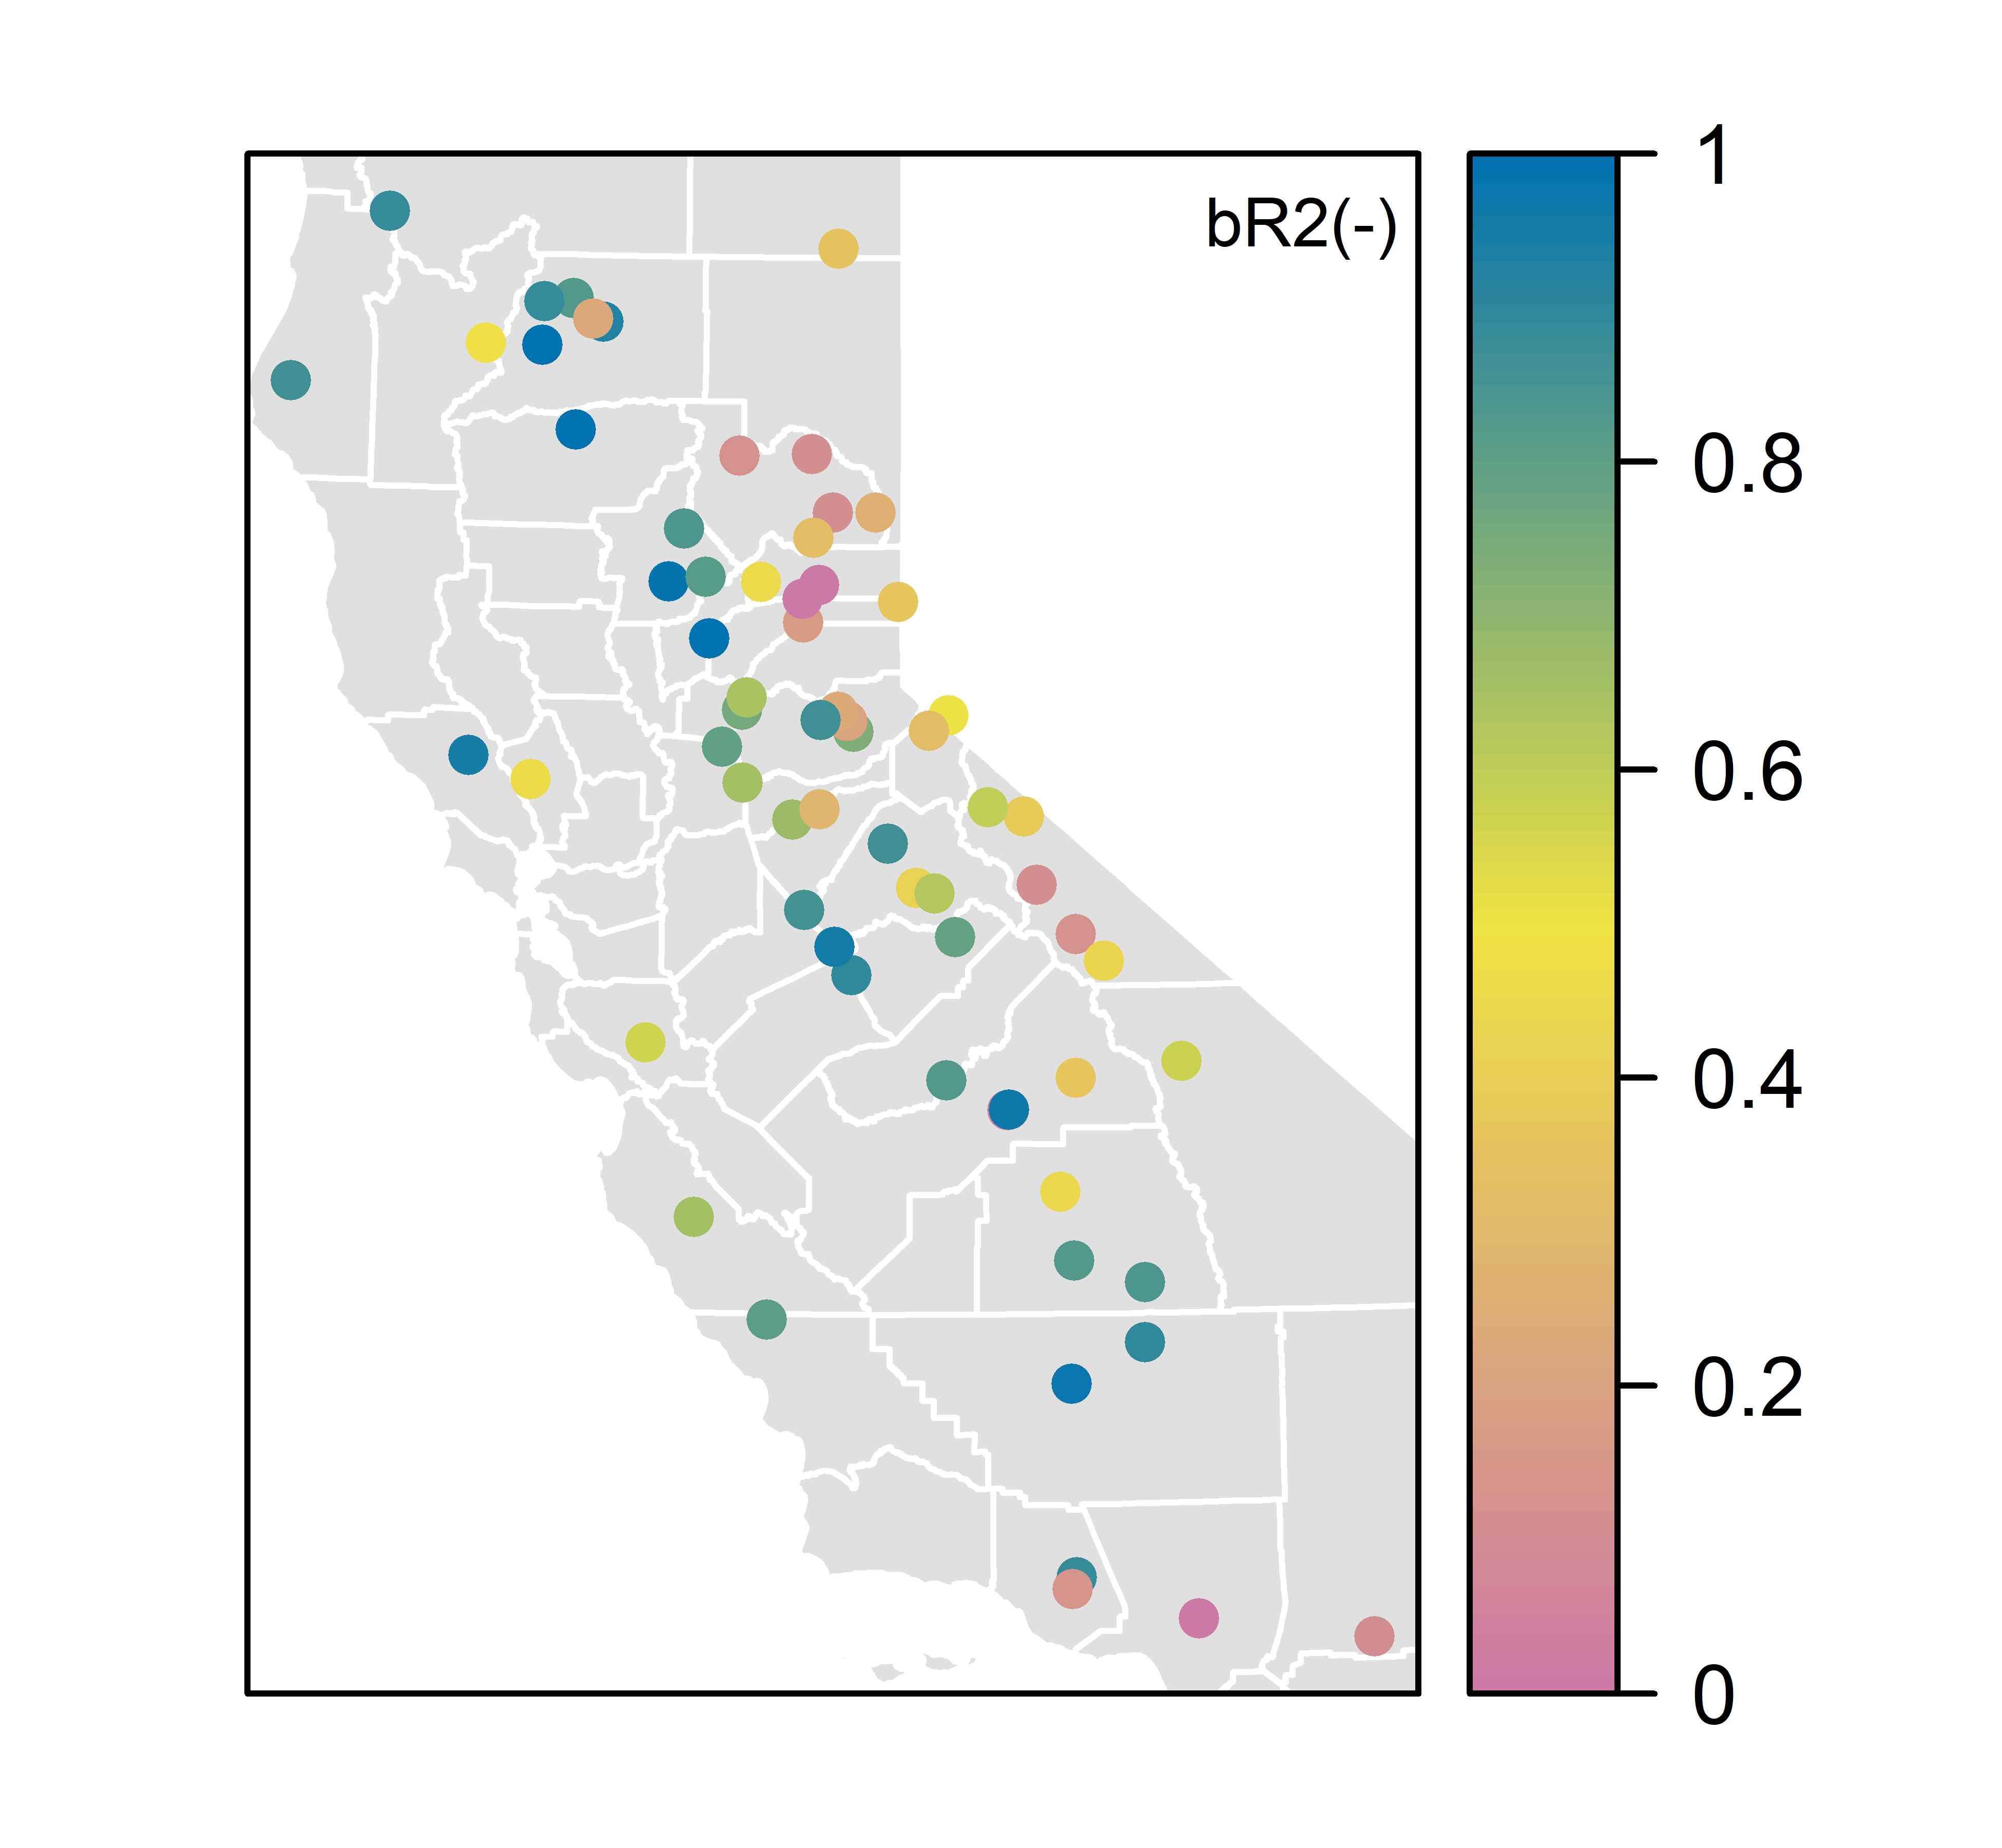
\includegraphics[width=\textwidth, trim={0 0 0 0}, clip=true]{plots/rplot28_br2map_nn_inc.png}
  		\caption{Test Set Error}
	\end{subfigure}% 
	\begin{subfigure}{.5\textwidth}
  		\centering
 		 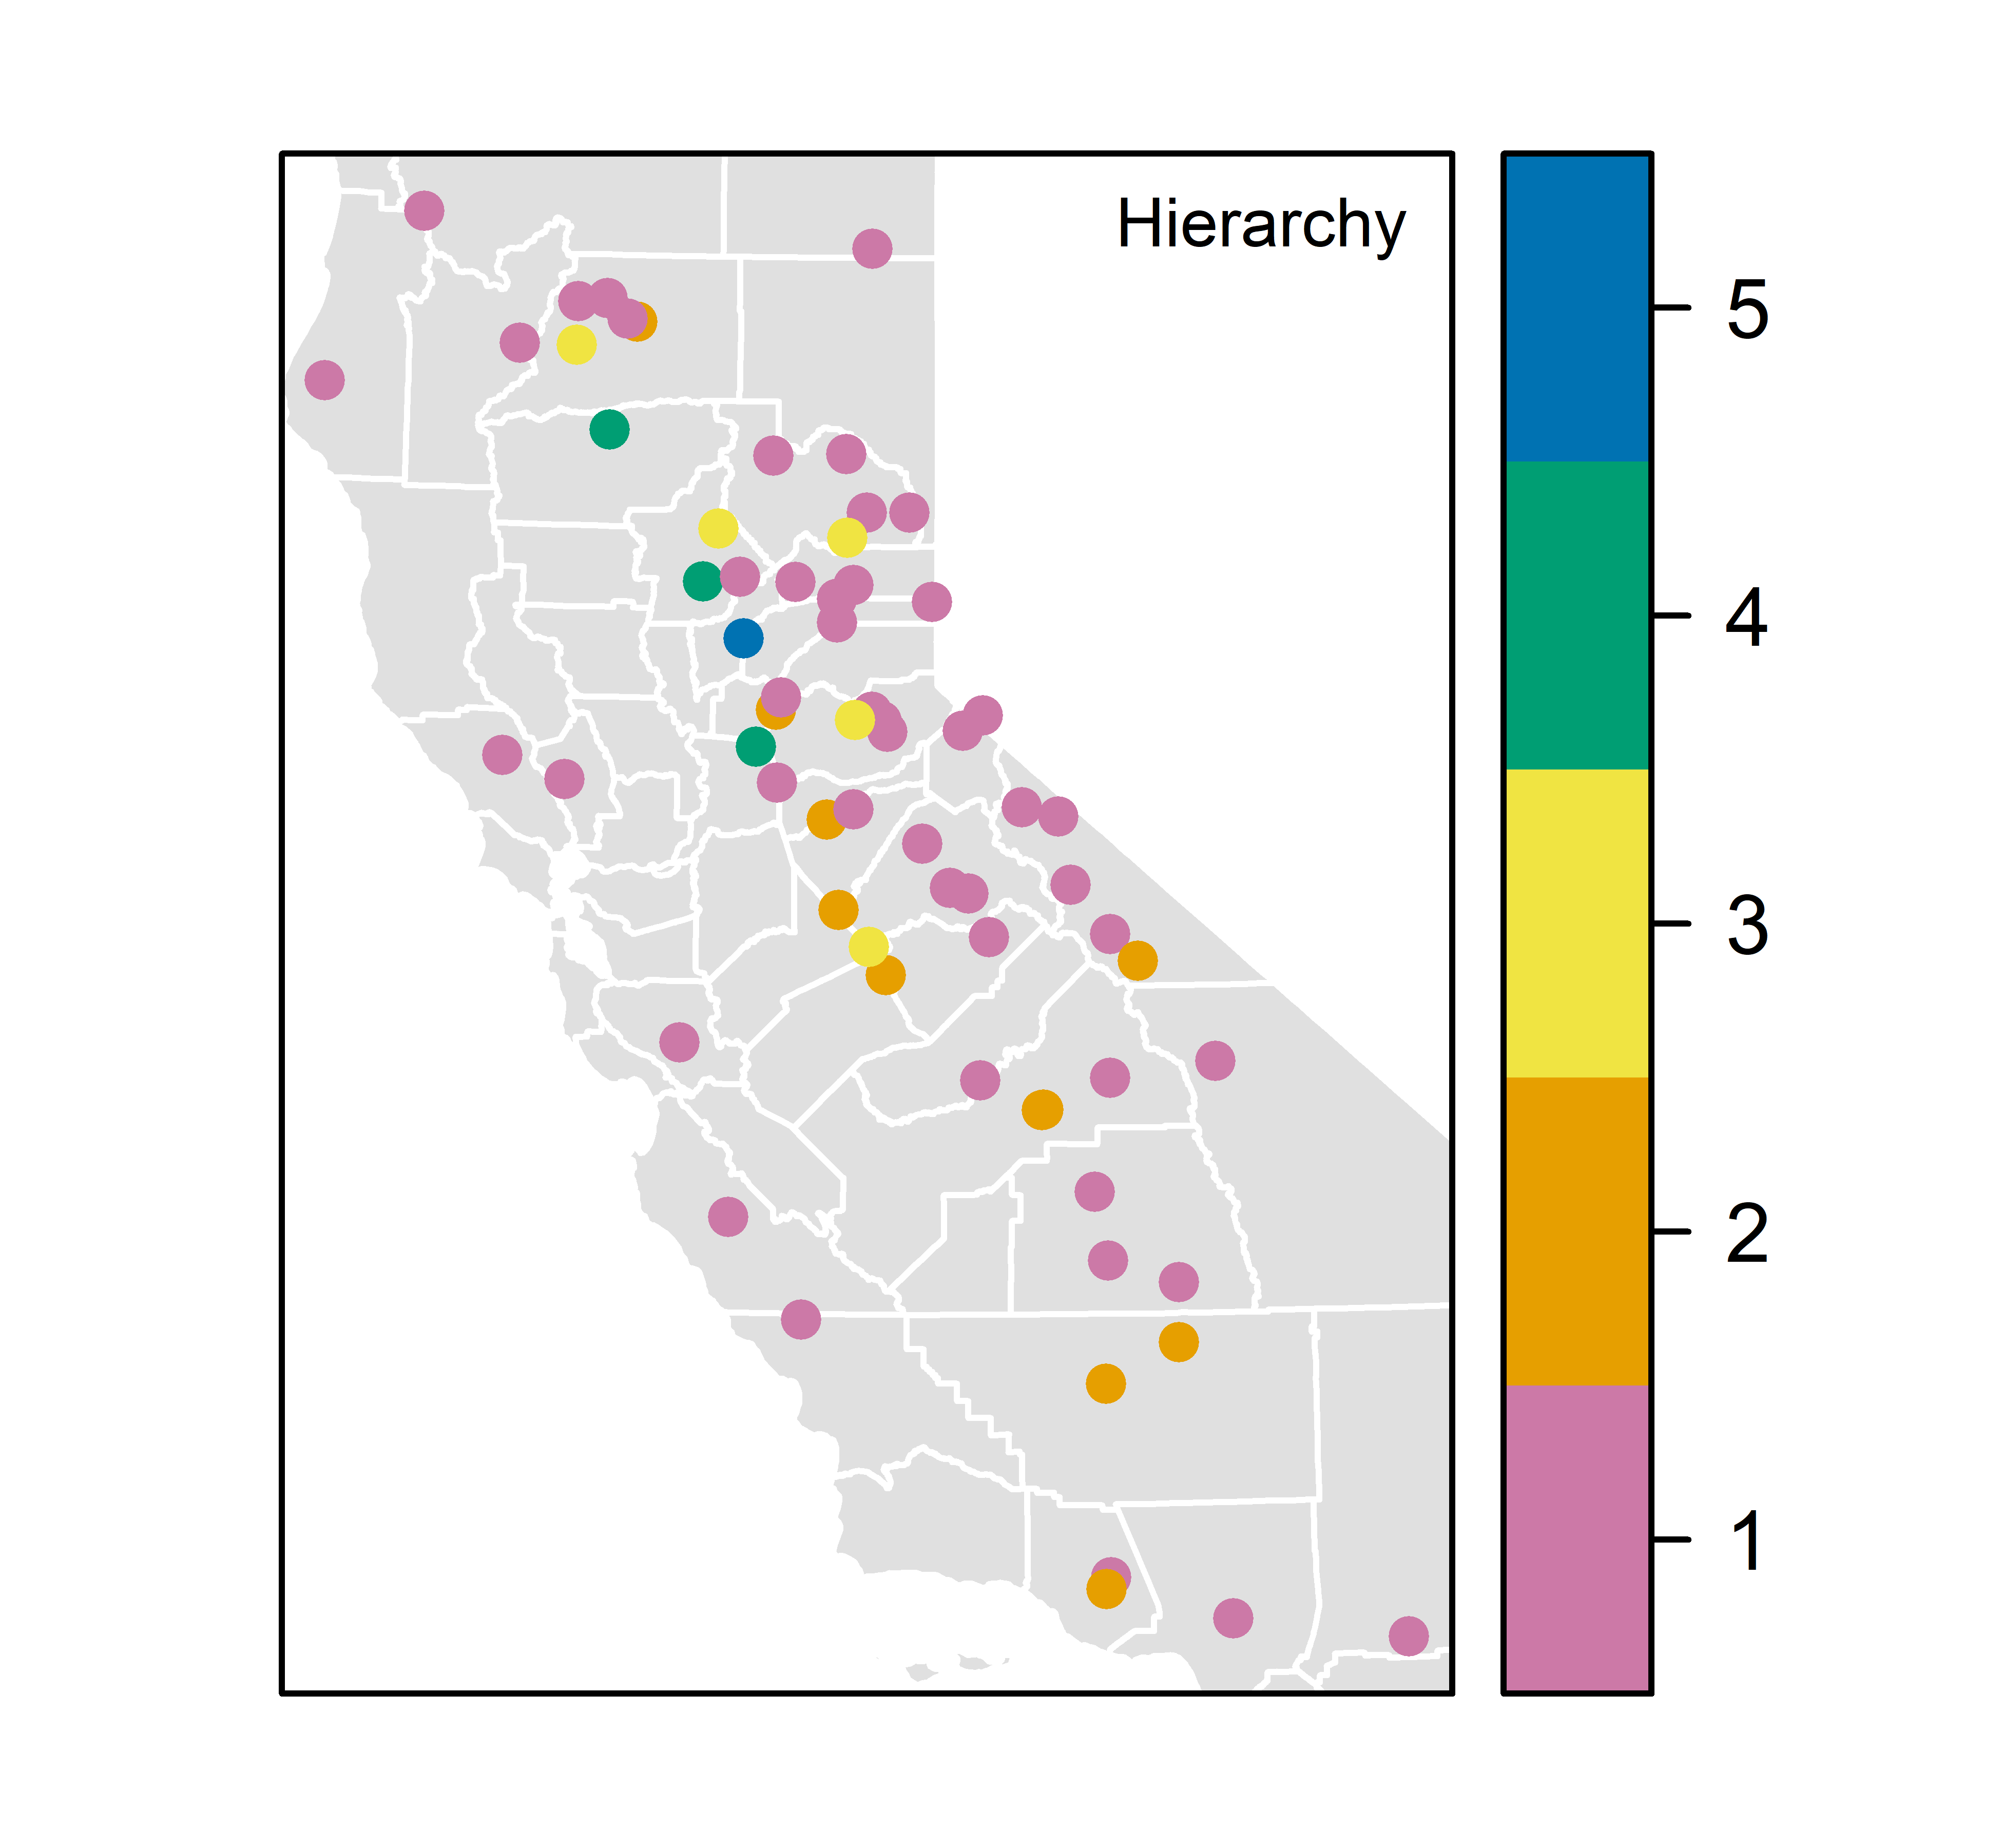
\includegraphics[width=\textwidth, trim={0 0 0 0}, clip=true]{plots/rplot210_hierarchies.png}
  		\caption{Basin Hierarchies}
	\end{subfigure}% 
	\hfill
	\caption{The spatial distribution of errors. (a) The bR\textsuperscript{2} error is not random and follows a line down the middle of California, and it somewhat follows the basin hierarchies. (b) The basins are not evenly distributed between the hierarchies; the lower the hierarchy the more basins in this study. Altogether, the lower the basin is in the network (i.e., the higher its hierarchy), the better the model performs.}
	\label{fig:incbr2plus}
\end{figure}

\begin{figure}
	\centering
	\begin{subfigure}{.5\textwidth}
  		\centering
 		 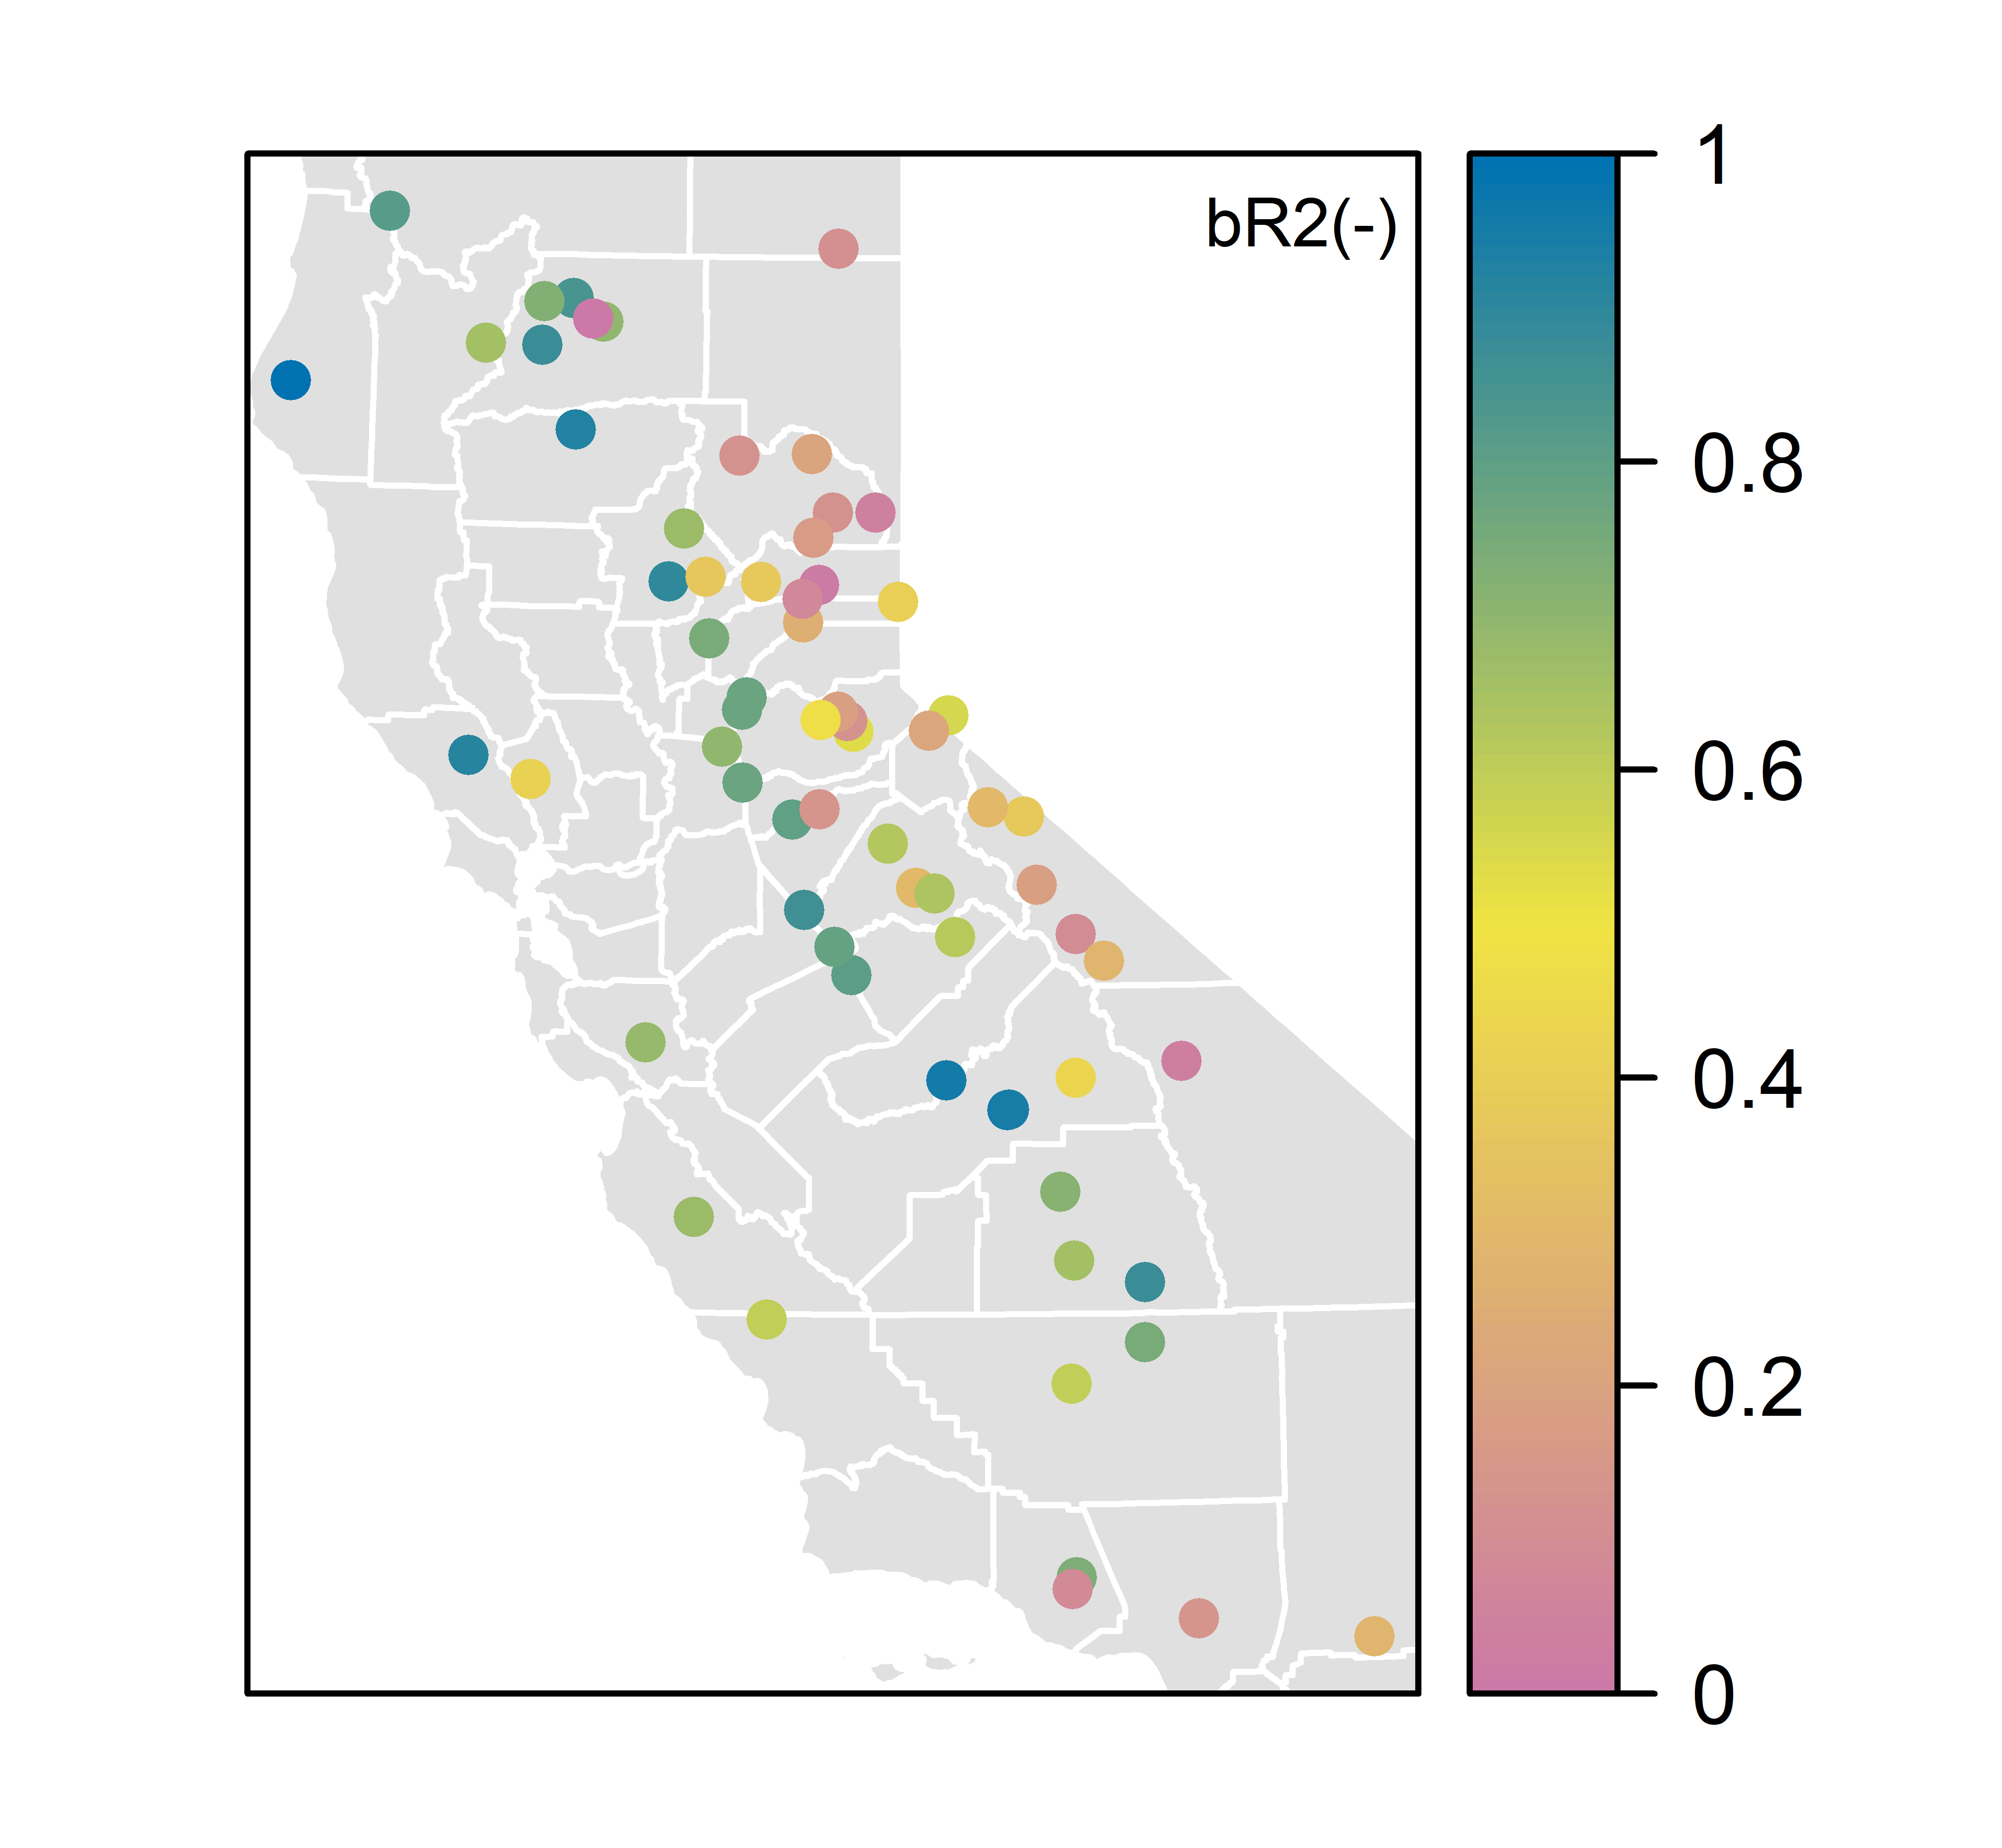
\includegraphics[width=\textwidth, trim={0 0 0 0}, clip=true]{plots/rplot28_br2map_nn_agg.png}
  		\caption{NN Aggregate}
	\end{subfigure}% 
	\begin{subfigure}{.5\textwidth}
  		\centering
 		 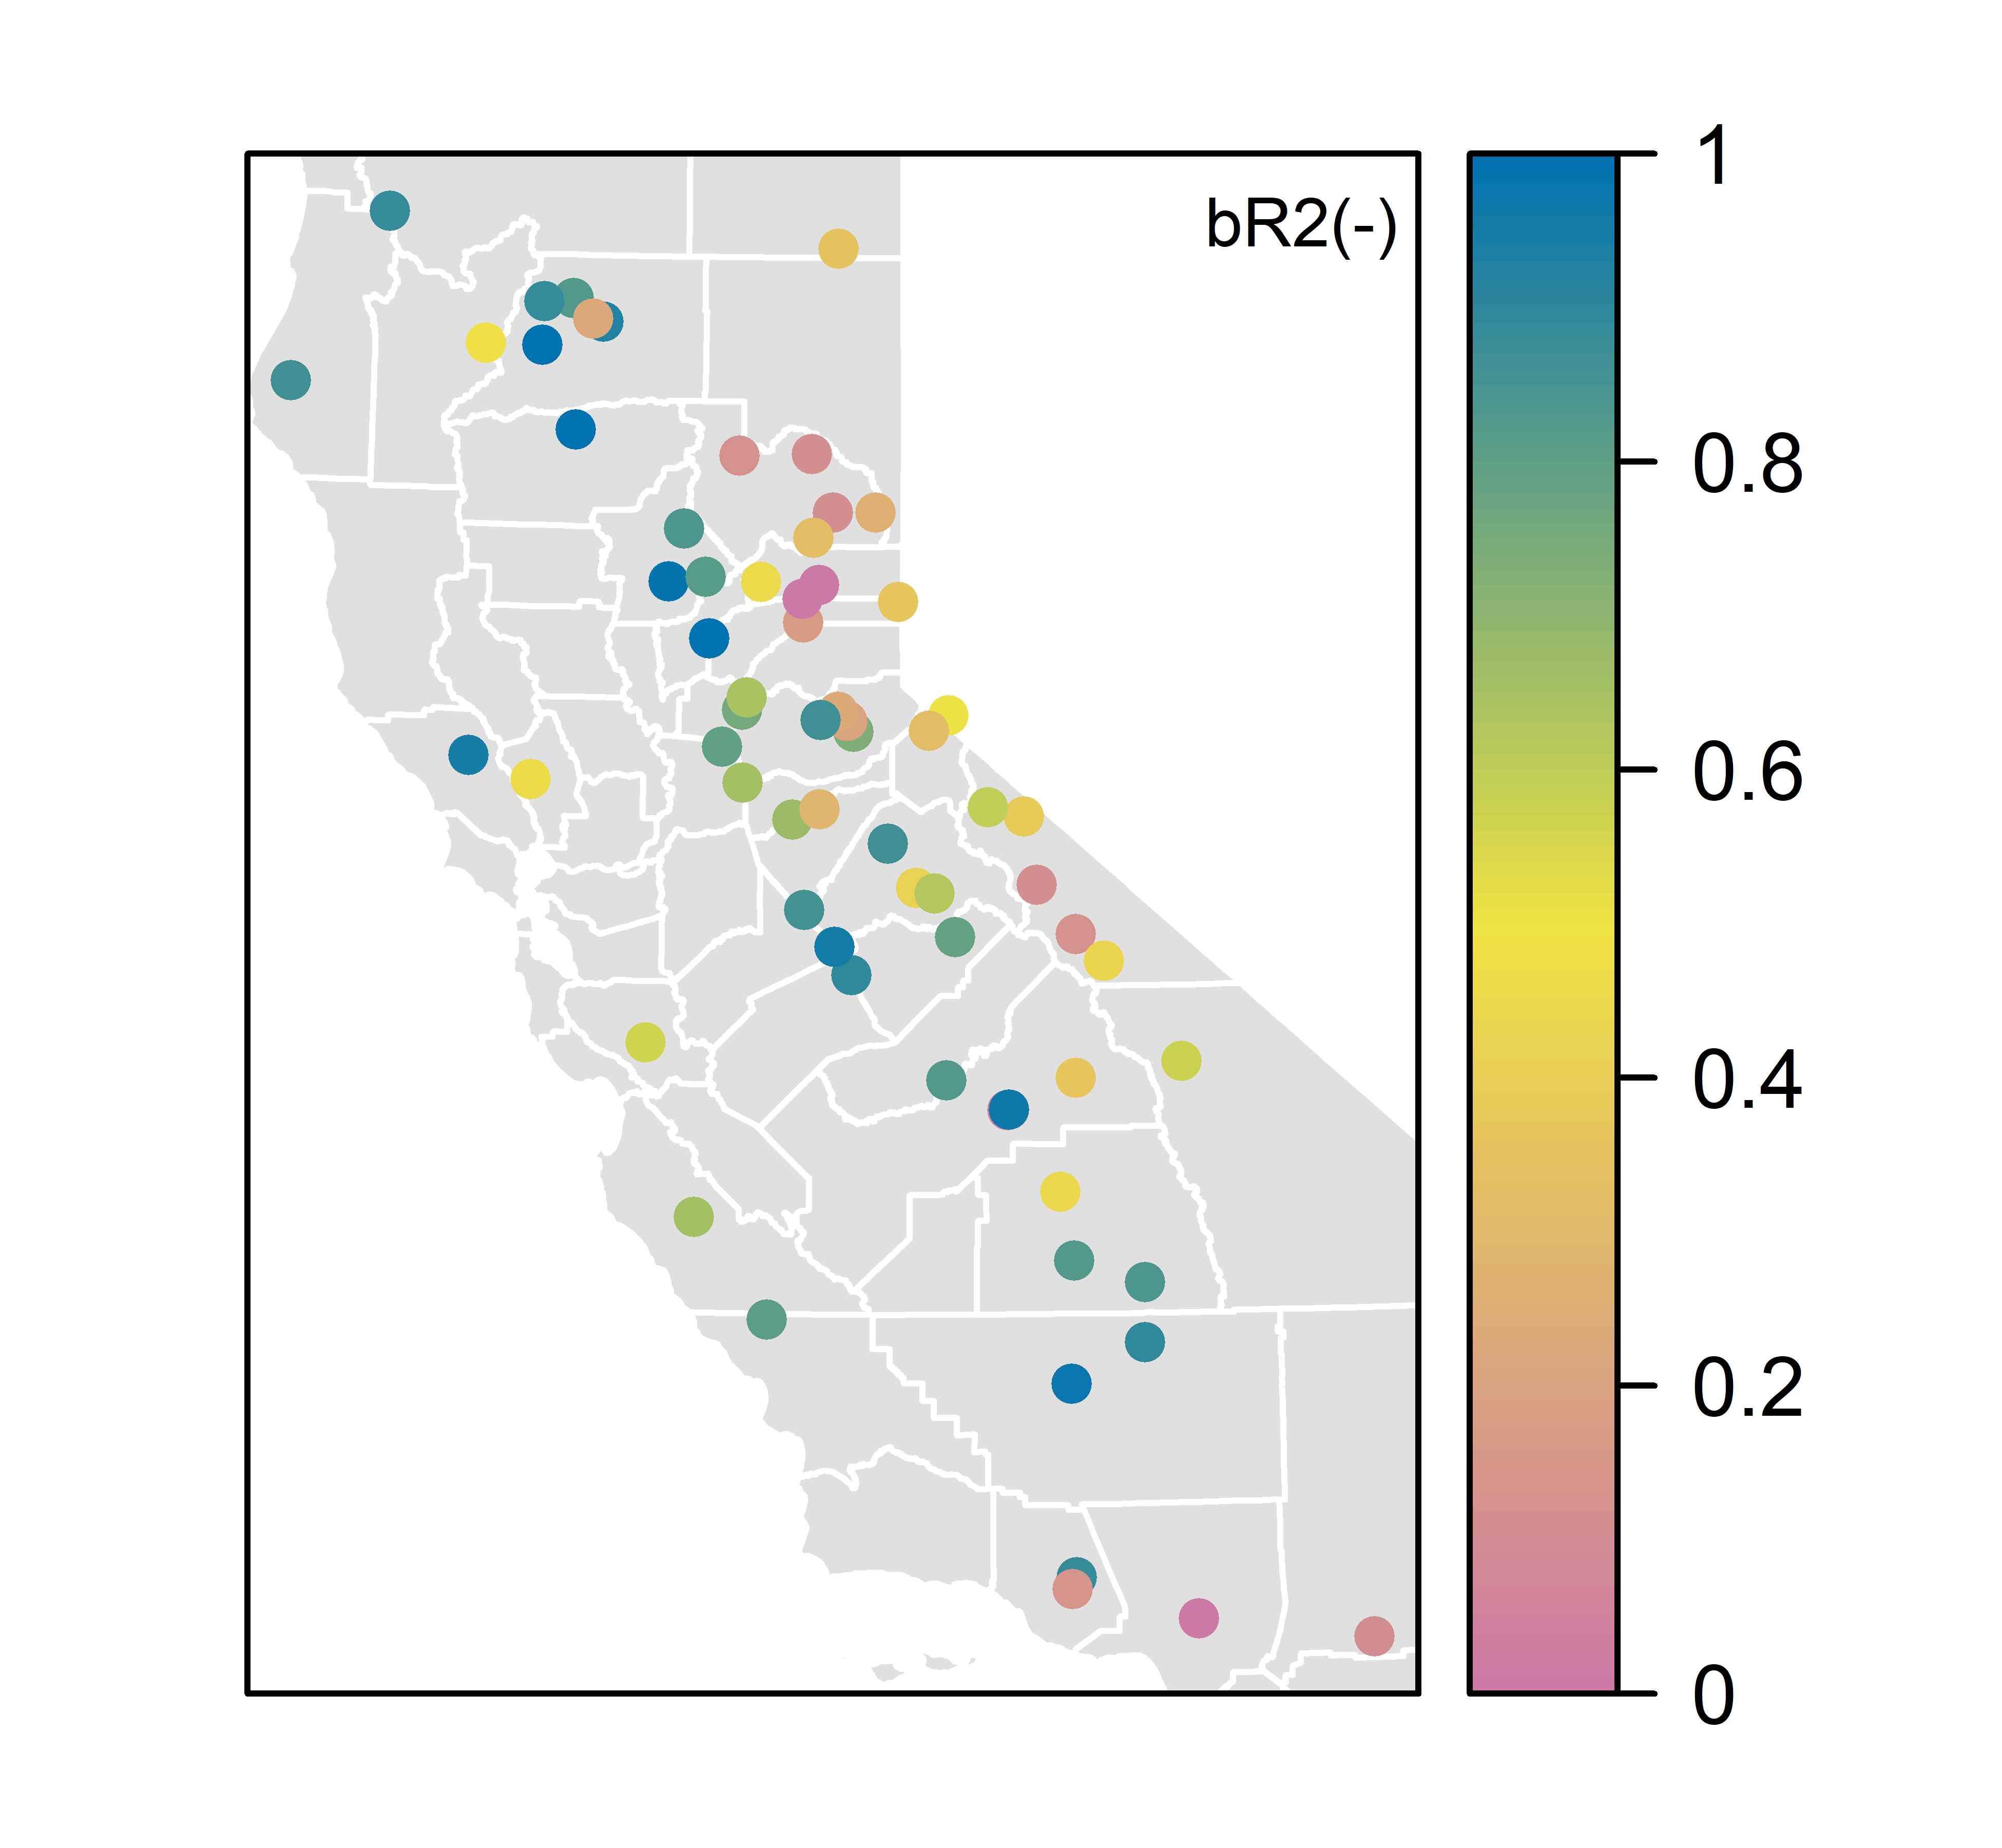
\includegraphics[width=\textwidth, trim={0 0 0 0}, clip=true]{plots/rplot28_br2map_nn_inc.png}
  		\caption{NN Incremental}
	\end{subfigure}% 
	\hfill
	\caption{The aggregate and incremental basins perform very similarly when there isn't any information upstream (i.e., hierarchy=1). However, when we introduce information upstream (i.e., hierarchy=2,3,4, and 5) the incremental basins can perform much better than the aggregate.}
	\label{fig:aggincbr2comp}
\end{figure}

Figures \ref{fig:br2dotchartcomp} and \ref{fig:br2boxplotcomp} show that when there is no flow information upstream (i.e., hierarchy=1) there is not much difference in the performance of incremental and aggregate models. However, when we introduce increasingly more information upstream (i.e., hierarchy=2,3,4, and 5) the NN incremental model can perform much better than the NN aggregate model. Even though the data set is smaller in the basins lower in the network, we can conclude that, the model is performing better at these basins due to information upstream and not just due to its higher flows and the loss function. 

\begin{figure}
  	\centering
 	 \includegraphics[width=0.9\textwidth, trim={0 0 0 0}, clip=true]{plots/rplot211_bR2dotchart_comp.png}
  	\caption{Basin bR\textsuperscript{2} performance in order.}
  	\label{fig:br2dotchartcomp}
\end{figure}

\begin{figure}
  	\centering
 	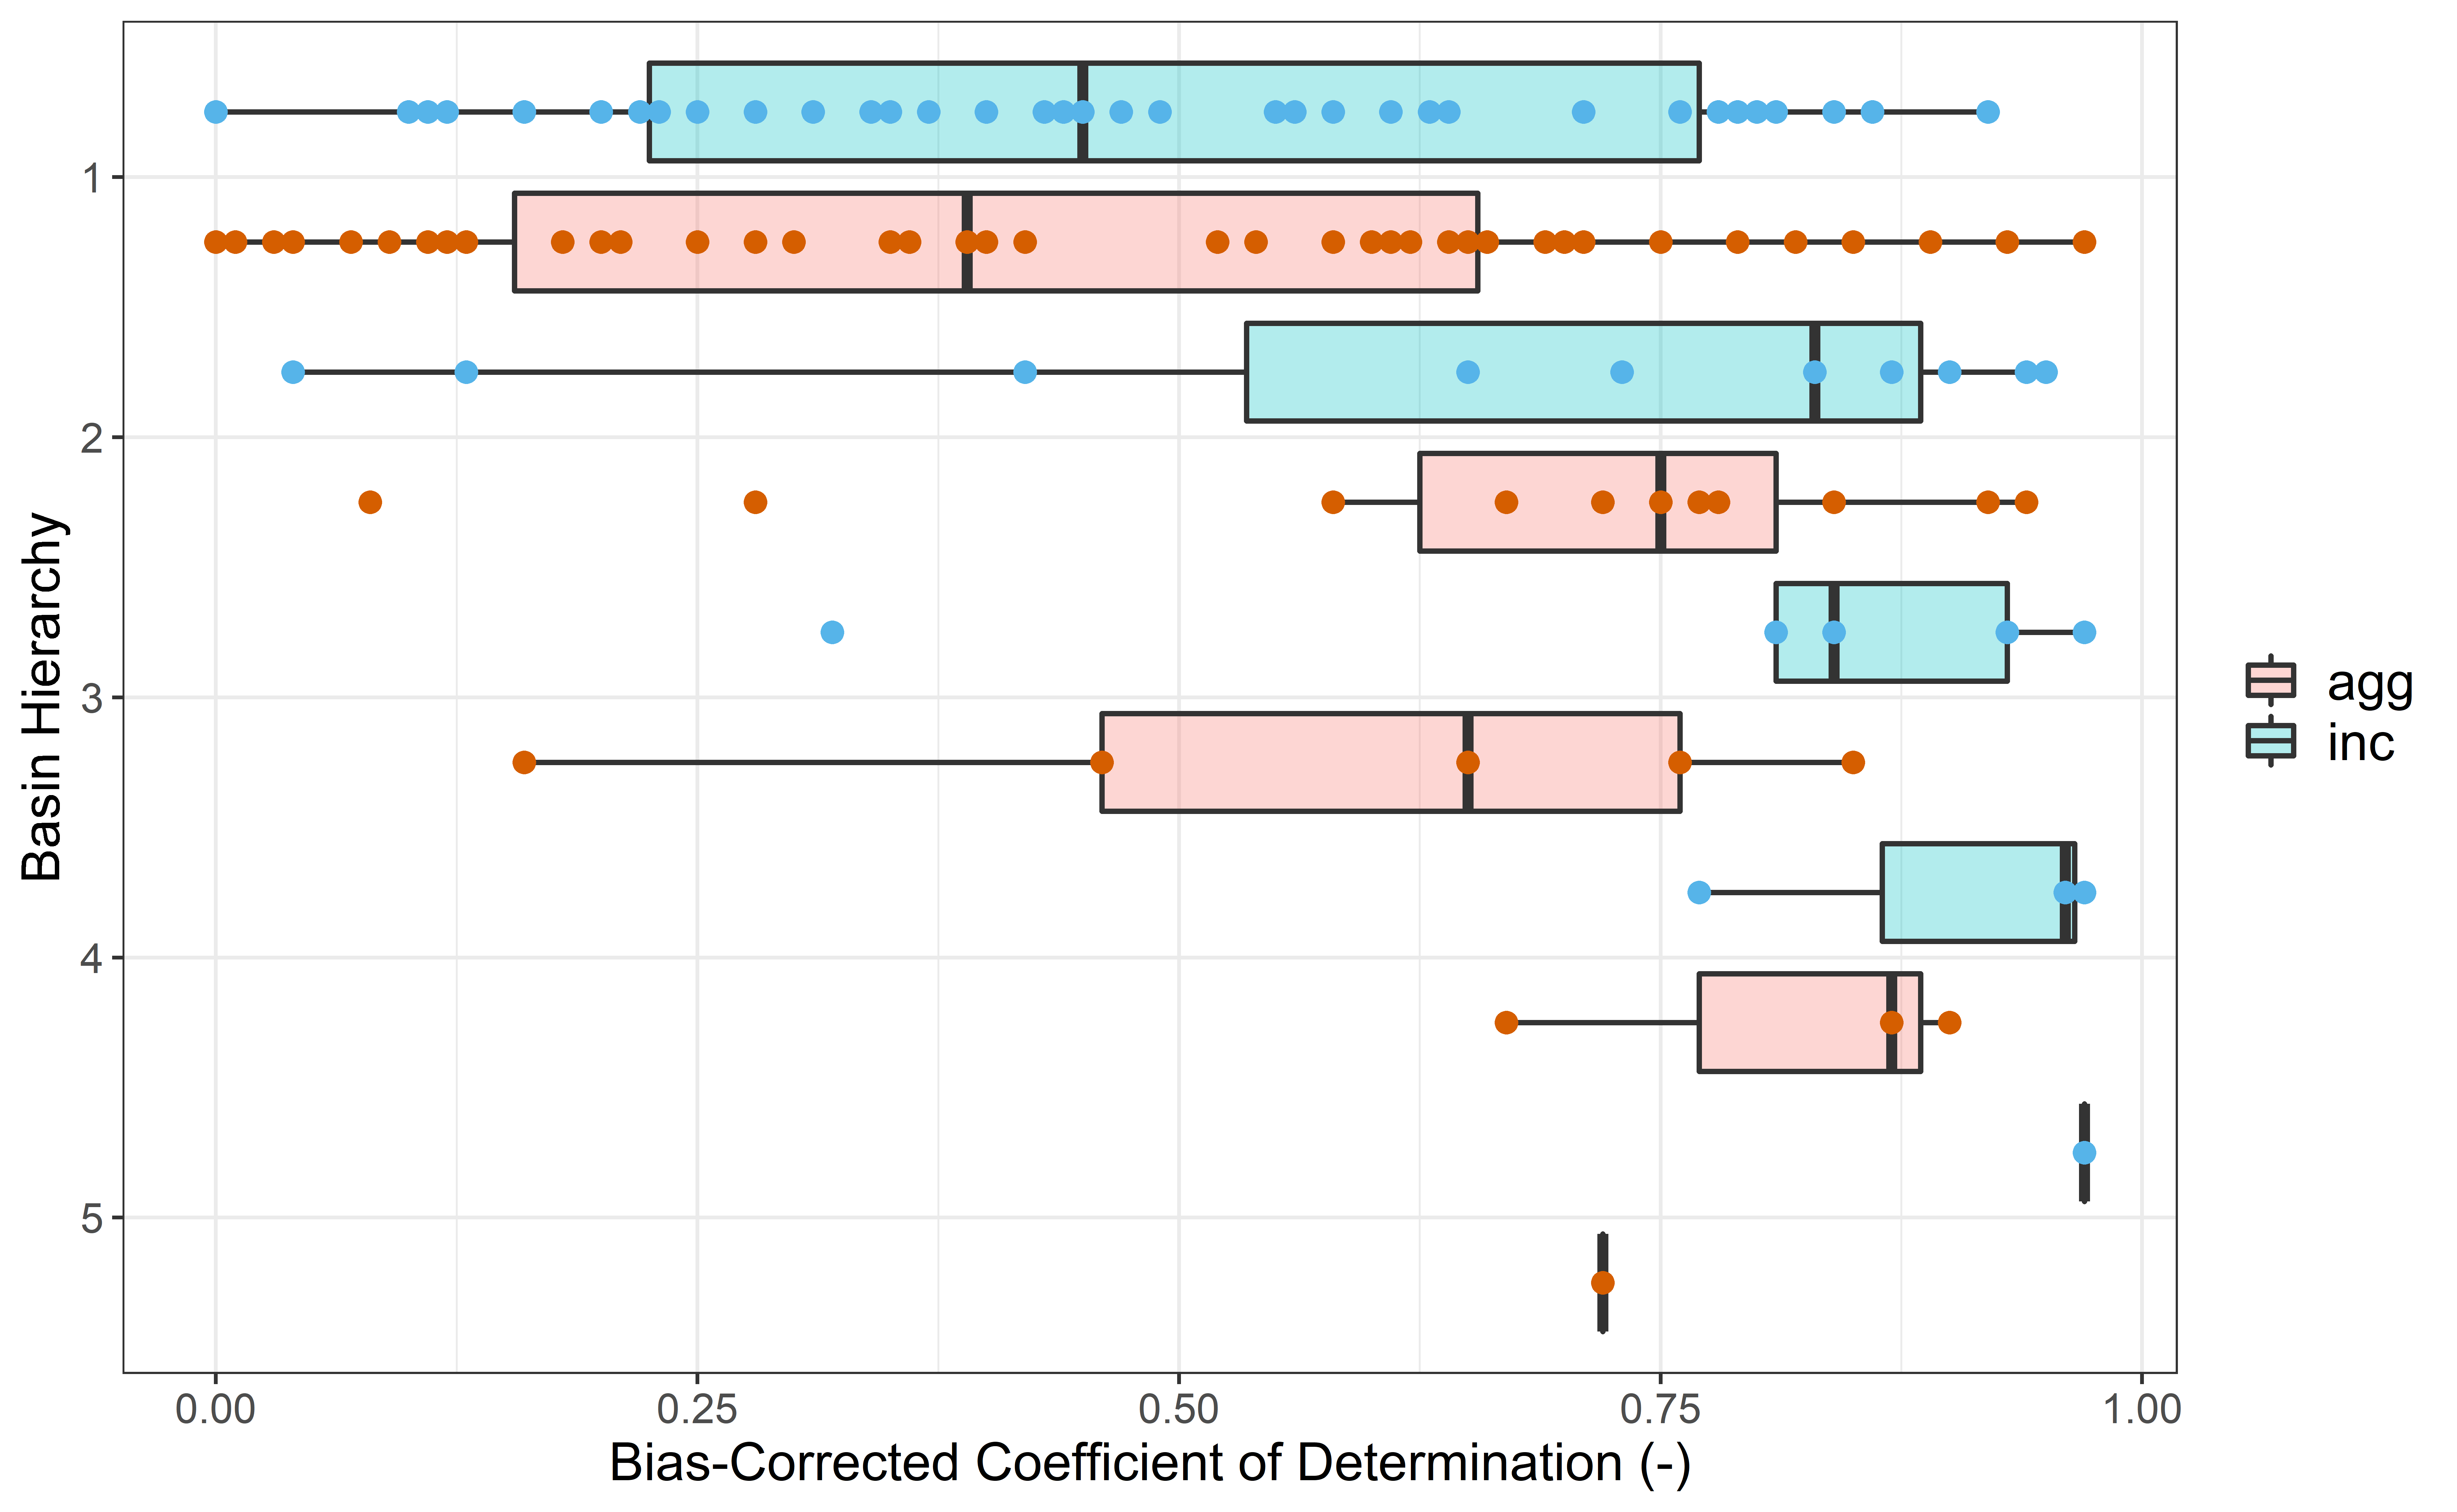
\includegraphics[width=0.8\textwidth, trim={0 0 0 0}, clip=true]{plots/rplot212_bR2gofboxplot_comp.png}
	\caption{The incremental and aggregate basins perform very similarly when there is no information upstream (i.e., hierarchy=1). However, when we introduce information upstream (i.e., hierarchy=2,3,4, and 5) the incremental basins can perform much better than the aggregate.}
	\label{fig:br2boxplotcomp}
\end{figure}

%------------------------------------------------------------------------------------------------------------------------------------------------------------------------
\section{Conclusion}
Incremental basin modeling provides an easy way to include network information in statistical models and the results show that it is valuable for modeling hydrology with parametric models especially those that have a few parameters like the LM and GLM. As the results showed, the LM and GLM prefer the incremental modeling approach, whereas the RF and the NN are somewhat insensitive to it. 

On this data set, and according to the performance ratings provided by \citeA{Moriasi2007885}, the GLM and RF provide a ``good" prediction for unimpaired flows, and the NN provides a ``very good" one (Table \ref{table:modelperformance}). We can hypothesize that the RF performed well due to the nature of non-parametric methods where the model form is determined by the data and hence the data is ``honored" and prediction becomes easier. The NN performance is the best and proves why these methods are so popular in studies in hydroinformatics. 

\begin{table*}[h]\renewcommand{\arraystretch}{1} 
	\linespread{1.0}
	\centering
	\caption{Model performance ratings. Criteria are given by \protect\citeNP{Moriasi2007885} (Appendix \ref{d:mof}).}
	\begin{tabular}{p{5cm}p{5cm}p{5cm}} % must add to 16.5
		\toprule
		Model & Aggregate & Incremental  \\
		\midrule
		LM & Unsatisfactory & Satisfactory \\
		\addlinespace
		GLM & Unsatisfactory & Satisfactory \\
		\addlinespace
		RF & Good & Good \\
		\addlinespace
		NN & Very Good & Very Good \\
		\bottomrule
	\end{tabular}
	\label{table:modelperformance}
\end{table*}

In another experiment, the models were trained on their cumulative flows and cumulative rainfall. Given that snow-melt driven hydrology dominates the Sierra-Nevada basins, and processing the data to its cumulative forms would have given the model a ``memory" effect, we repeated the experiment in this chapter with cumulative values. However, surprisingly, none of the models were able to provide satisfactory results, and therefore, we have therefore left those results out of this chapter. 

The next chapter will explore one flaw we pointed out here: the squared loss function forcing better predictions at flood levels at the expense of drought level data. We will be training models using different asymmetric loss functions to penalize the under predicting of floods and over predicting of droughts at a higher cost (i.e., forcing the model to reach the peaks and valleys of the hydrograph). 


\chapter[New Loss Functions]{New Loss Functions: Comparing Asymmetric and Symmetric Methods of Evaluating Error} \label{ch3:loss}
\chaptermark{New Loss Functions}
\setlength{\epigraphwidth}{4.5in}
\epigraph{Maybe all one can do is hope to end up with the right regrets.}{Arthur Miller, \textit{``The Ride Down Mount Morgan''}, 1991}

%----------------------------------------------------------------------------------------------------------------------------------------------------------------------------------------------------------
\section*{Summary}
In practice, the loss function for a chosen statistical learning method is the translation of a informal philosophical objective into the formal language of mathematics \cite{hennig2007some}. Therefore, the choice of a loss function in estimation is somewhat subjective and depends on the specific application of the model or the decisions being made when using it. Some loss functions have already been established in and are common in hydrology. 

This chapter will look at differences in performance of already established and new functions in hydrology when they are embedded in the machine learning algorithm rather than using them as only an evaluation step after the model is built. 

%----------------------------------------------------------------------------------------------------------------------------------------------------------------------------------------------------------
\section{Introduction}
% add literature review here
Mechanistic models in hydrology simulate conditions based on available input parameters, modeled processes, and calibration to specific locations. \textit{Measures-of-fit} or the similarity of the simulations to the observations help in assessing model performance. Visual similarity is recommended first (i.e., the plot of observed and simulated time series), and calculated measures-of-fit are recommended next. In model calibration, these measures can help guide better fits of simulations to observations.  

In statistical learning, the same process can be used by estimating the model using a pre-defined loss function, solve the simulation problem as well as is possible, and then calculate the model measures-of-fit of interest. However, improving a model trained on a different loss function than that which is desired can be quite tricky. Since the machine learning algorithm requires a loss function to begin with, we can directly define the custom loss function as the measure-of-fit of interest before deploying the learning algorithm. This section performs statistical learning with different loss functions, and then examines the differences in predictions. 

Typical loss functions in statistical learning are the $\ell1-norm$ and $\ell2-norm$ (See Equation \ref{eq:l1} and \ref{eq:l2}). The $\ell2-norm$ is the familiar objective function in simple least-squares regression, a convex function, emphasizing points distant from the bulk of the data. % (i.e., data points that have high leverage and can influence the model more than other points).

\begin{equation} \label{eq:l1}
	\ell_1(y_i,\hat{f}(x_i)) = ||y_i-\hat{f}(x_i)||_1 = \abs{y_i-\hat{f}(x_i)} 
\end{equation}
	
\begin{equation} \label{eq:l2}
	\ell_2(y_i,\hat{f}(x_i)) = ||y_i-\hat{f}(x_i)||_2^2 = \left(y_i-\hat{f}(x_i)\right)^2 
\end{equation}
 
% IS THIS TRUEEEEEEE? 
% If we use equation \ref{eq:l1}, the algorithm will try to correctly predict the median correctly, and if we use equation \ref{eq:l2}, the algorithm will try to correctly predict the mean. Both imply that the modeler is more concerned with the measures of centrality than predicting the extremes of the distribution more accurately.

\textit{Risk}, or cost, is defined as the expectation of the loss function. For example, the risk of over predicting the severity of a drought can be defined as \textit{how much} it was over predicted on average. This distance can be defined as the absolute value of the difference or the difference squared as in Equations \ref{eq:l1risk} and \ref{eq:l2risk}, the empirical risks associated with the  $\ell1-norm$ and $\ell2-norm$. The expectation of the $\ell2-norm$ will produce a model that regresses to the mean, and the $\ell1-norm$ regresses to the median. That is, the $\ell2-norm$ is more sensitive to outliers than the $\ell1-norm$.

\begin{equation} \label{eq:l1risk}
	\begin{aligned}
		& L_1(y_i,\hat{f}(x_i)) = E\left[\ell_1(y_i, \hat{f}(x_i))\right] = \frac{1}{n} \sum_{i=1}^{n} \abs{y_i-\hat{f}(x_i)}
		% E\left[\abs{y_i-\hat{f}(x_i)}\right] \\
		% & L\left(\abs{y-\hat{f}(x)}\right) = \frac{1}{n} \sum_{i=1}^{n} \abs{y_i-\hat{f}(x_i)}
	\end{aligned}
\end{equation}
	
\begin{equation} \label{eq:l2risk}
	\begin{aligned}
		& L_2(y_i,\hat{f}(x_i)) = E\left[\ell_2(y_i, \hat{f}(x_i))\right] = \frac{1}{n} \sum_{i=1}^{n} {(y_i-\hat{f}(x_i))^2}
		% E\left[(y_i-\hat{f}(x_i))^2\right] \\
		% & L\left((y-\hat{f}(x))^2\right) = \frac{1}{n} \sum_{i=1}^{n} {(y_i-\hat{f}(x_i))^2}
	\end{aligned}
\end{equation}

On the other hand, \textit{Regret} is the difference between the consequences of a sub optimal decision and the optimal decision. Often, in reinforcement learning, the objective is to minimize regret, which is equivalent to maximizing the highest accumulated reward \cite{sutton2018reinforcement}. For example, maybe over predicting the severity of a drought this year will lead to better management of resources and fewer regrets in later years.

In this research, to avoid developing a mathematical representation for regret, we leave this discussion and proceed with the much simpler \textit{risk-minimization framework} (See Equation \ref{eq:mlriskmin}). 

\begin{equation} \label{eq:mlriskmin}
	\hat{f}(x_i) = \underset{\tilde{f}}{\mathrm{argmin}} \ E\left[L(y, \tilde{f}(x))\right] \\
\end{equation}
%----------------------------------------------------------------------------------------------------------------------------------------------------------------------------------------------------------
\section{Research Design} \label{ch4:design}
This study used the monthly unimpaired flows data set developed and maintained by the California Data Exchange Center (CDEC). Unimpaired flow is the flow produced by the basin in its current state, but, without dams and diversions \cite{cadwruf2016}. 

The data spans 69 California basins (See appendix \ref{d:ufdataset}, Figure \ref{fig:map}) from 1982 to 2014. It can be downloaded with the {\tt sharpshootR} package in R \cite{beaudette2016package}. 28 predictor attributes were calculated for each observation point based on the knowledge of basin characteristics and processes that influence a watershed's response to precipitation: evaporation (temperature); snowfall (cumulative sum of precipitation below 2$^{\circ}$C); storage in soil (with soil and land cover parameters); antecedent conditions (with lagged precipitation and temperature parameters); and groundwater processes (with geology and depth to a restricted layer) (See Table \ref{table:ufvariables}). The dataframe has approximately 18,500 monthly unimpaired flow observations in acre-feet (AF) and as a continuous variable can be used for regression type studies. 
% subset of the data, we just need to investigate the loss function. 
% Could be interesting to use the temperature dataset for this chapter too.
%Since we are just examining the loss function, the developed dataset is much smaller

Typical measures-of-fit developed in hydrologic modeling are the Mean Absolute Error (MAE), Relative Standard Deviation (RSD), Relative Mean (RMU), Mean Squared Error (MSE), Root Mean Square Error (RMSE), normalized RMSE (nRMSE), RMSE standard deviation ratio (RSR), Percent Bias (PBIAS), Coefficient of Determination (R$^2$), Nash-Sutcliffe Efficiency (NSE), Index of Agreement (d), Modified NSE, Modified d, Relative NSE, Relative d, King-Gupta Efficiency (KGE), and Volumetric Efficiency (VE). appendix \ref{e:mof} presents their equations, strengths, and weaknesses. First, let us consider a list of characteristics that the loss function, in its application to hydrologic prediction, should fulfill:

(1) \textbf{Should the loss function be symmetric?} In symmetric functions, under predicting produces the same loss as over predicting of the same absolute error. However, a conservative loss function applies a different penalty to the different directions of loss. That is, an asymmetric loss function can force the model to over predict the severity of floods and droughts rather than under predict them. This approach requires the labelling of all instances of the data as either a peak, normal, or drought point, requiring a labeling mechanism (i.e., a classification model) before running the predictive regression model. 

Great care should be taken not to introduce ``data leakage'', or the leakage of information from the response variable into the final predictive model; the classification model will have to either be trained on the predictor variables only, or use a portion of the data that is thrown away for the rest of the study. A simple classification model can be defined by a fit of a thin plate spline to the precipitation data with a predefined degree of smoothness (i.e., degree of freedom). Next, we find the points at which the direction of curvature (the second derivative) in the time series changes. Areas where the curvature is upward can be labelled drought and downward labelled flood. 

After all data points are labeled, we define two asymmetric loss functions for each peak and valley section (See Figure \ref{fig:asymmetric1}). Such loss functions can be defined as linear exponential (LINEX) loss if smoothness is desired (See Equation \ref{eq:linex}). However, current subgradient-based and derivative-free methods of optimization in convex programming can easily handle non-differentiability at the origin of the loss function. In fact, many asymmetric loss functions in machine learning have a simple \textit{kink} in them, which makes them otherwise entirely differentiable. Figure \ref{fig:asymmetric3} and Equation \ref{eq:asshinge} explain such a function. % For a definition of terms see appendix \ref{a:terms}. 

\begin{figure}[ht]
	\centering
	\begin{subfigure}{.5\textwidth}
  		\centering
 		 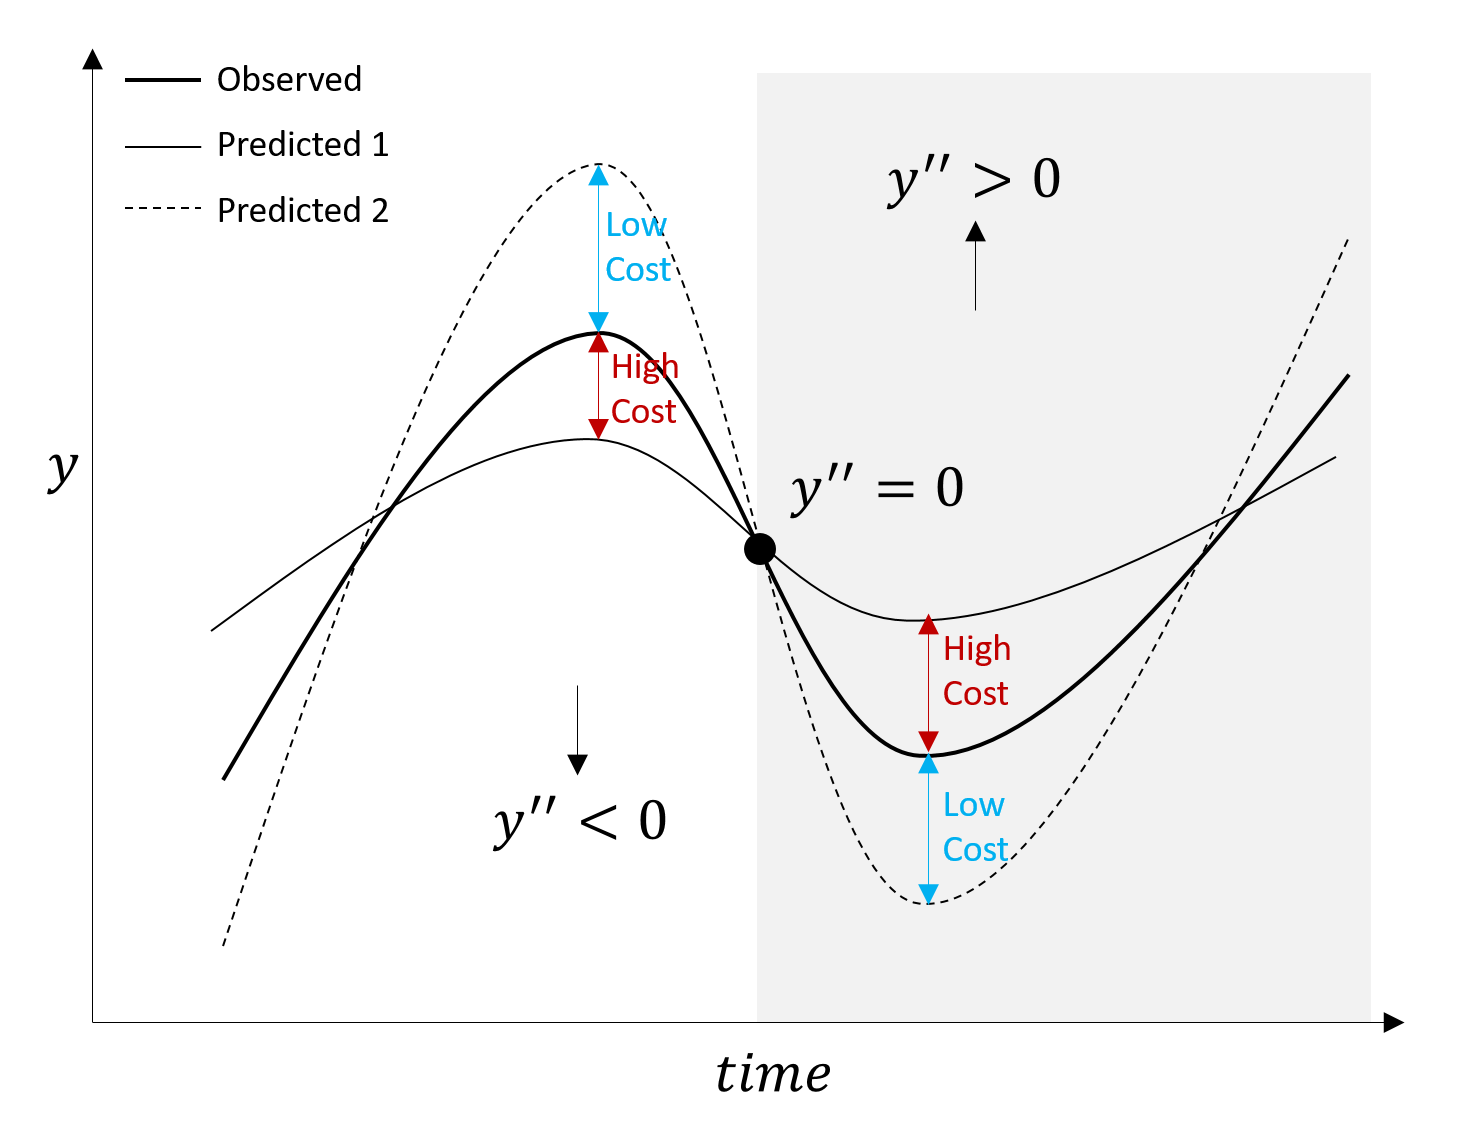
\includegraphics[width=\textwidth, trim={0 0 0 0}, clip=true]{plots/asymmetric1_a.png}
  		\caption{Asymmetric loss shown around peaks and valleys.\newline}
  		\label{fig:asymmetric1a}
	\end{subfigure}% 
	\begin{subfigure}{.5\textwidth}
  		\centering
  		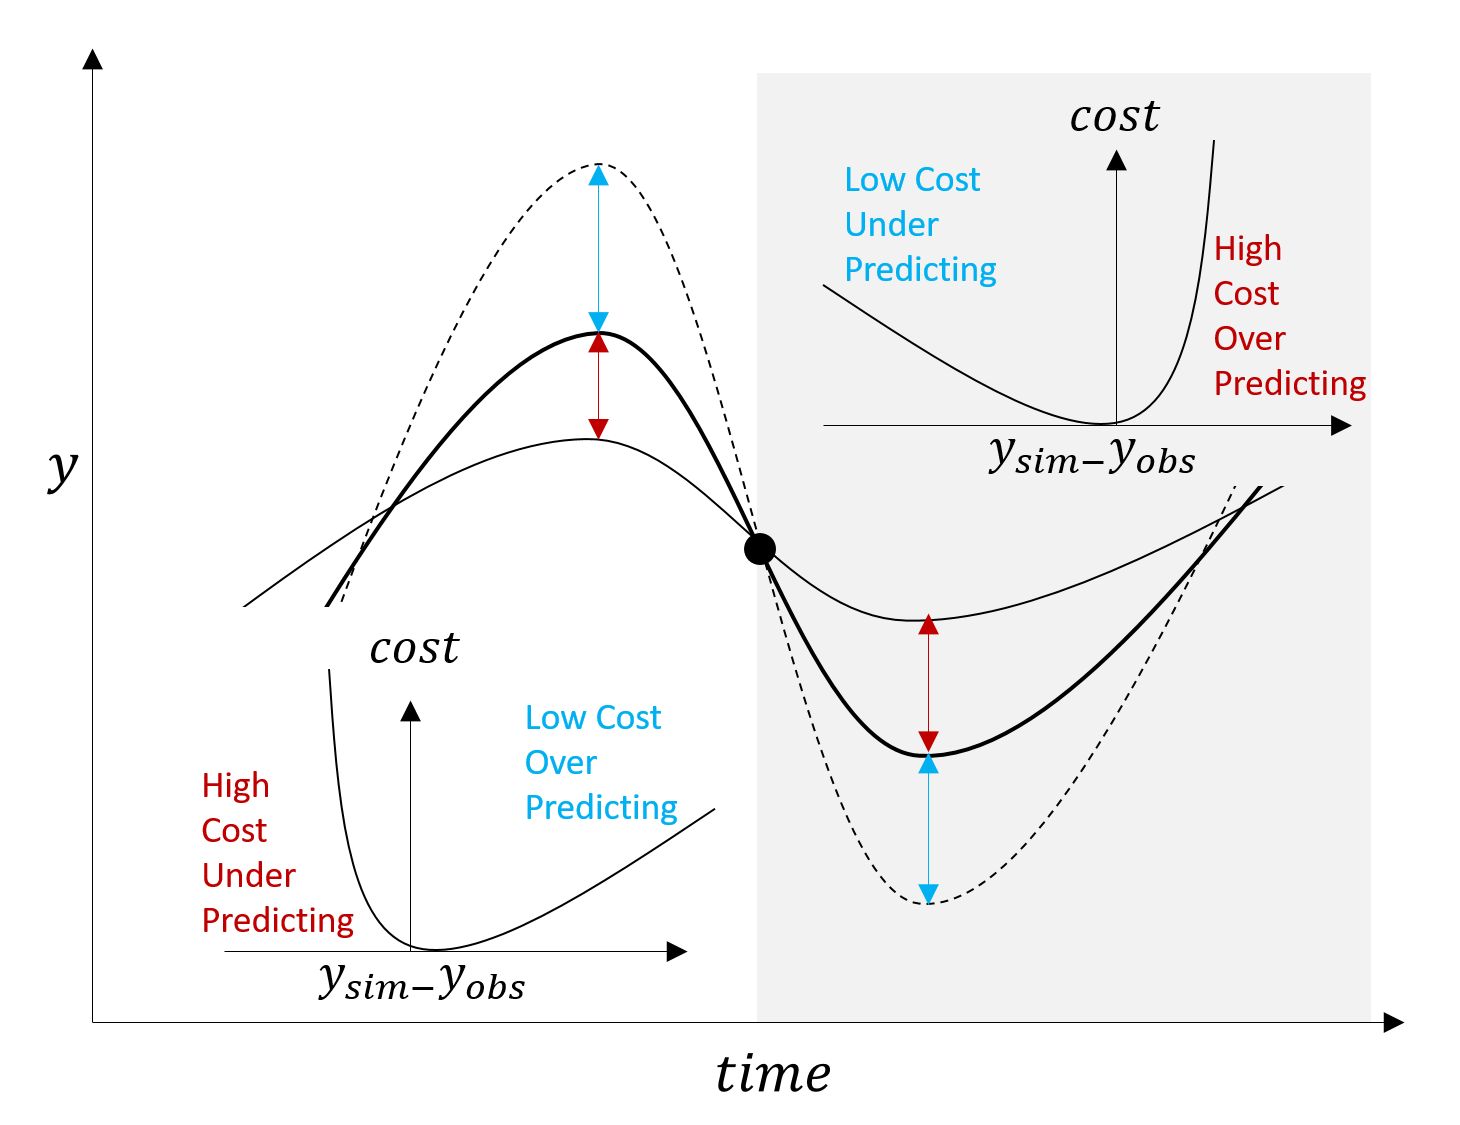
\includegraphics[width=\textwidth, trim={0 0 0 0}, clip=true]{plots/asymmetric1_b.png}
  		\caption{Asymmetric loss can be defined with LINEX functions.}
  		\label{fig:asymmetric1b}
	\end{subfigure}
	\caption{Asymmetric loss functions define different losses to over predicting and under predicting a value.}
	\label{fig:asymmetric1}
\end{figure}

\begin{equation} \label{eq:linex}
	LINEX(y_i,\hat{f}(x_i)) = e^{\phi(y_i-\hat{f}(x_i))} - \phi(y_i-\hat{f}(x_i))-1, \quad\text{$\phi$} \in \mathbb{R}
\end{equation}

\begin{figure}[ht]
	\centering
 	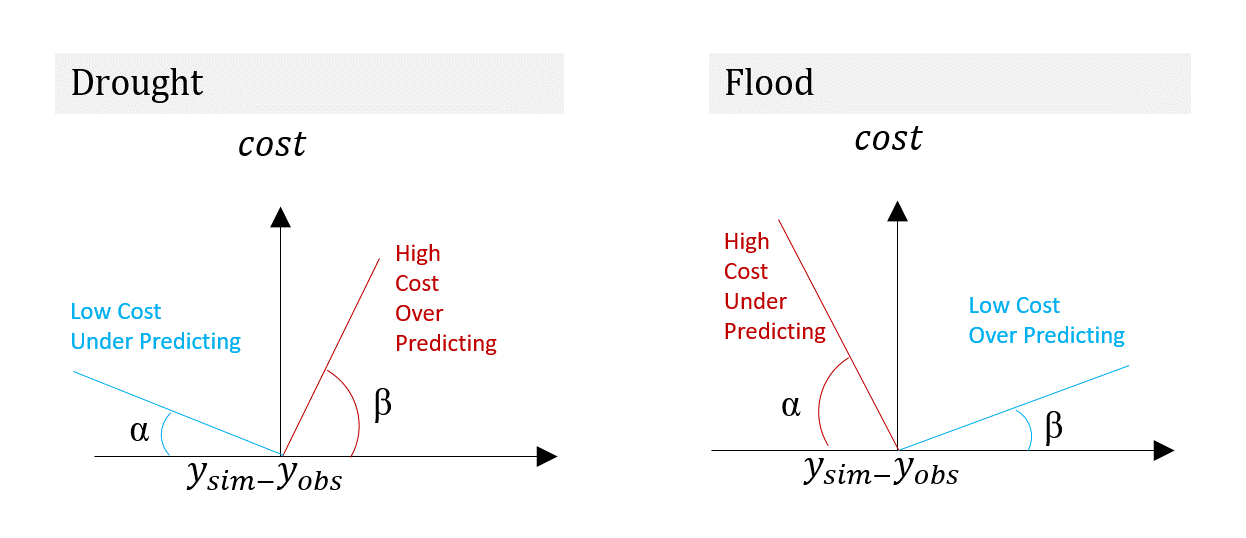
\includegraphics[width=0.8\textwidth, trim={0 0 0 0}, clip=true]{plots/asymmetric3.png}
	\caption{Asymmetric loss functions define different losses to over predicting and under predicting a value.}
	\label{fig:asymmetric3}
\end{figure}

\begin{equation} \label{eq:asshinge}
	Hinge(y_i,\hat{f}(x_i)) = \alpha*min(0, \hat{f}(x_i)-y_i)+ \beta*max(0, \hat{f}(x_i)-y_i)
\end{equation}

The squared error loss penalizes larger errors more than smaller error (i.e., the function is steeper in the tails than in the middle). To preserve this feature we can combine the concepts above and define a weighted $\ell2-norm$ (See Equation \ref{eq:weightedse}). 

\begin{equation} \label{eq:weightedse}
	Weighted\ Squared\ Error(y_i,\hat{f}(x_i)) = \alpha*\left[min\left(0, (\hat{f}(x_i)-y_i)\right)\right]^2+ \beta*\left[max\left(0, (\hat{f}(x_i)-y_i)\right)\right]^2
\end{equation}

%Also, we could develop a cost function that penalized a standard deviation ratio (See Equation \ref{eq:rsd}) greater than one more than it does the same measure when it is less than one (See Figure \ref{fig:asymmetric2}). Such a cost function will ensure we make more conservative decisions as over predicting extremes is valued over under predicting them.  
%
%\begin{figure}
%	\centering
%	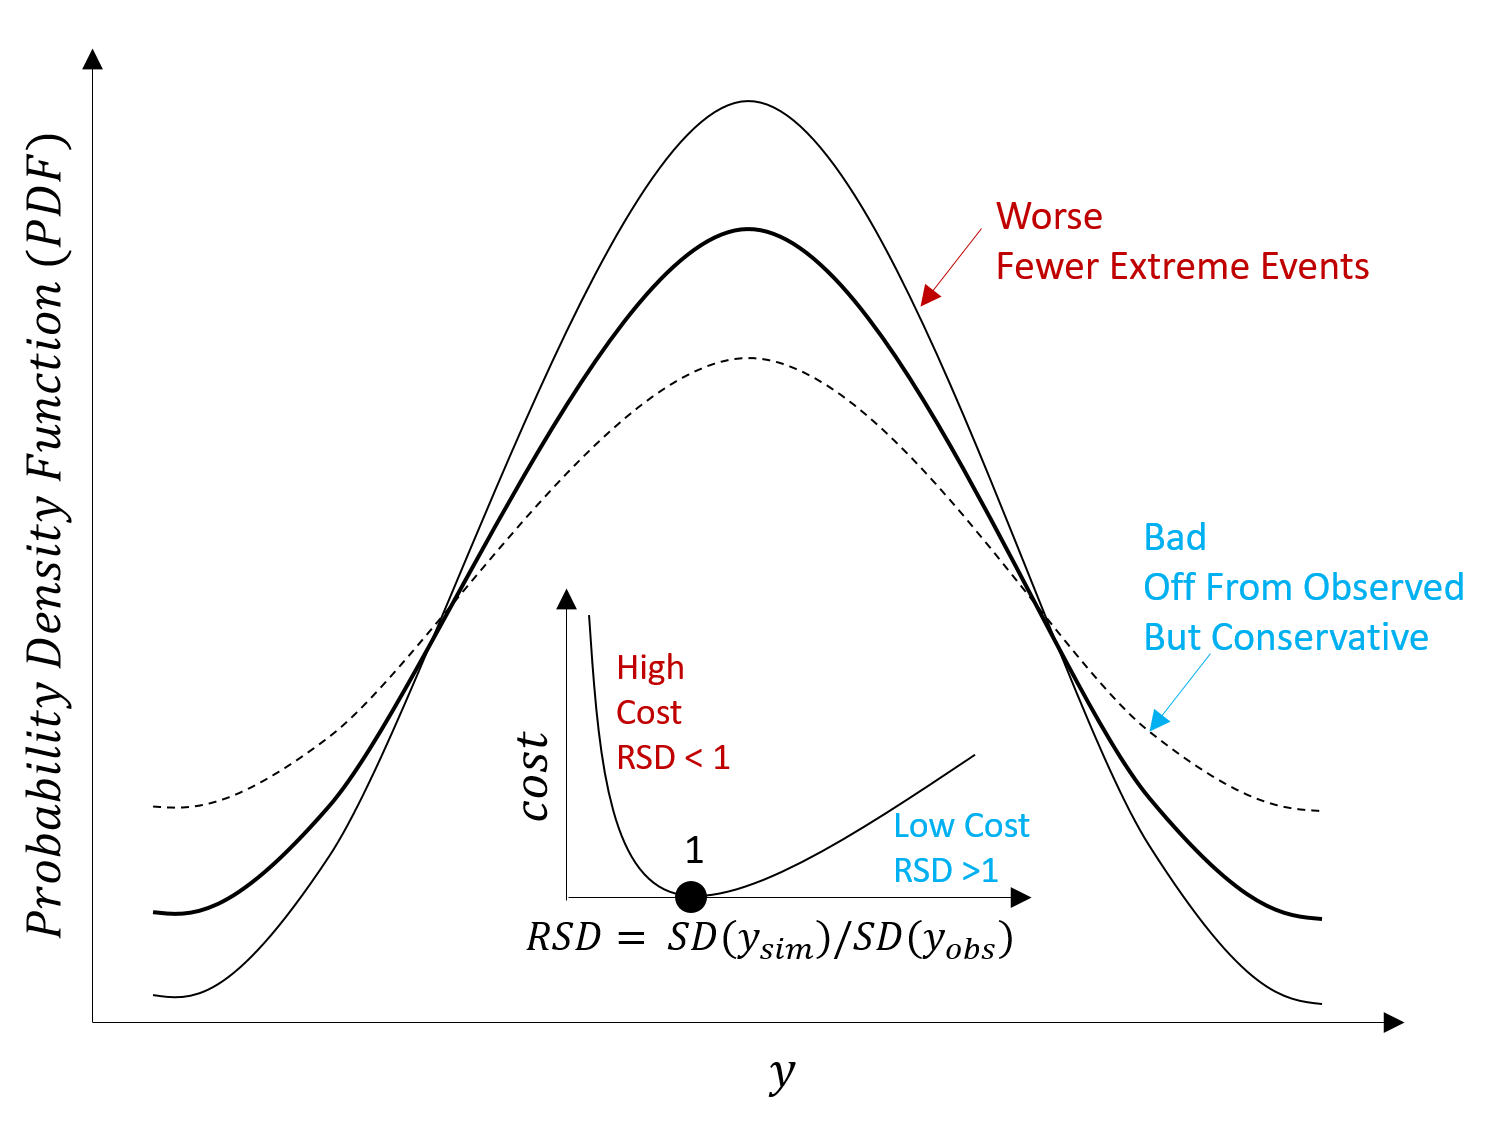
\includegraphics[width=.5\textwidth,trim={0 0 0 0},clip=true]{plots/asymmetric2.png}
%	\caption{ blah blah blah blah  blah blah blah blah  blah blah blah blah  blah blah blah blah  blah blah blah blah  blah blah blah blah} 
%	\label{fig:asymmetric2}
%\end{figure}

(2) \textbf{Should we be concerned with relative errors or absolute errors?} In hydrology, both manual and automatic attempts aimed at minimizing absolute errors often lead to fitting the higher portions of the hydrograph (i.e., peak flows) at the expense of the lower portions (i.e., baseflow) \cite{krause2005comparison}. Relative errors are generally more important than absolute errors. For example, a 10 TAF error in 1,800 TAF (monthly annual average of the Sacramento River) is less extreme of an error than in 15 TAF (monthly annual average of the Colorado River). Relative error loss functions or a simple log transformation of the data can help in this regard. 
% studentized, standardized by mean or sd? how are these different? 
% although for the matter for water supply then the absolute values are important not relative. 

(3) \textbf{Should losses be a continuous function, or stepwise?} Although, most outcomes may follow a discontinuous step function (e.g., a neuron firing or not), many decisions in water resources (e.g., releases from a reservoir) are continuous. Continuity and differentiability make continuous math more convenient. One major development in neural networks was doing away with the concept of thresholds in the step function (representing the collective influence of all the inputs) and replacing it with a smoother \textit{sigmoid} function. As with neural networks, many optimization algorithms require continuity and differentiability (e.g., gradient decent). However, advances in these methods now allow for piece-wise differentiability in the loss function.
% many different shapes in the loss function.

(4) \textbf{Should losses be homogeneous or heterogeneous (i.e., weighted based on geographic region)?} The cost of incorrectly managing a densely populated urban basin may be very different than a desert or a headwater basin; the importance of having accurate flow estimates is not completely homogeneous especially across a big and diverse region as California. However, to avoid making those judgements, we will use a single loss function across all regions. 
% could use cost functions that differentiate between the costs of predicting the wrong hydrology for a populated basin and the same costs for fish species. % should costs from CALVIN? cost of not delivering the target demand. is that the same cost as not predicting the hydrology right? not really. 

\citeA{legates1999evaluating} suggests that a complete assessment of model performance should include at least one \textit{goodness-of-fit} or relative error measure (e.g., Modified NSE or Modified d defined in Equation \ref{eq:mnse} \& \ref{eq:md}, with $j=1$) and at least one absolute error measure (e.g., RMSE or MAE defined in Equation \ref{eq:rmse} \& \ref{eq:mae}) with additional supporting information (e.g., a comparison between the observed and simulated mean and standard deviations such as those defined in Equation \ref{eq:rsd} \& \ref{eq:rmu}) \cite{legates1999evaluating}. 

Therefore, along with the four characteristics discussed above, we propose to use only the following three selected measures-of-fit: the Modified NSE (as a relative error measure), the MSE and weighted MSE (as an absolute error measure), and the RSD (as an additional supporting measure). 

%-----------------------------------------------------------------------------------------------------------------------------------------------------------------------------------------------------
%\section{Preliminary Results} \label{ch4:results}
%A main feature of L2 is its convexity, which means that the differences
%between high prediction errors are assessed as more important than differences
%between small prediction errors.
%even if there are strong arguments in a particular situation
%that the loss function should be convex, it is almost always impossible to find
%decisive arguments why it should be exactly equal to L2.

%-----------------------------------------------------------------------------------------------------------------------------------------------------------------------------------------------------
\section{Conclusion} \label{ch4: conclusion}
This chapter will follow a risk minimization framework in developing a loss function. Contrary to other studies, we \textit{are putting the horse before the cart}. That is, the loss function is developed before performing the learning, not just as an evaluation step after. The different performances of the models will be compared against the loss functions applied. Next, we will compare the shape of the predictions in the time-series compared to the observations. In squared error loss functions (i.e., MSE, NSE) the peaks get fitted at the expense of the low flows (i.e., high leverage points). However, the proposed wighted squared error asymmetric loss may be able to force a fit to both tails of the distribution. A comparison of the results from these losses will determine whether the aforementioned problem is mitigated with asymmetric losses. A dissertation chapter will include a comparison between the results of various loss functions applied. It will investigate the differences in the general shape of predictions obtained across the various loss functions, and discuss the effects of different weights in the asymmetric weighted MSE function.   

%Surprisingly, the models perform vastly different from one another depending on the objective function used, highlighting the importance of this much overlooked step. In summary, we define what loss means to a certain problem, we use that as the objective function in the machine learning algorithm, and then perform the minimization. 

% happy models are all alike, every unhappy model is unhappy in its own way.  

% add the table made for presentation here. Complete this table and the chapter will be finished. 


\chapter[Rethinking Resampling Methods]{Rethinking Resampling Methods: Random Is Not Unbiased} \label{ch4:resampling}
\chaptermark{Rethinking Resampling Methods}
\setlength{\epigraphwidth}{4.5in}
\epigraph{If two things are similar, the thought of one will tend to trigger the thought of the other.}{Aristotle, \textit{``Laws of Association''}, 300 B.C.}

%----------------------------------------------------------------------------------------------------------------------------------------------------------------------------------------------------------
\section*{Summary}
After a statistical learning method is chosen and applied, the model needs to be tested. Most statistical learning techniques used in water resources modeling employ a randomized splitting of data into k-folds to estimate model error. In each iteration, one fold is held out as a test set and others are designated as a training set. Such random cross-validation methods ignore structures in the data, which underestimate model error  \cite{roberts2017cross}. % Also, models evaluated with randomized cross-validation methods disregard the assumption of independence of residuals. When mapping the residuals in time or in space, the trends point to dependence structures in the data that produce an over-fit model with non-causal parameters or missed meaningful parameters. %cite?

A more accurate estimate of the model error can come from techniques that block training sets in time, space, or unique structure (e.g., by hydrologic basins). The difficulty here lies in specifying block sizes in time and space. Blocking potentially reduces the range of parameters seen by the model, or may exclude a particular meaningful combination of predictor variables in the training data set. Too small of a block size and the cross-validation method more closely mimics the randomized method and runs the risk of under estimating model error. Large block sizes force too much model extrapolation and risk over estimating model errors. 

This chapter compares resubstitution, Monte Carlo (i.e., randomized), leave one group out (LOGO), and leave multiple groups out (LMGO) cross-validation strategies, as well as, resubstitution, Monte Carlo, blocked by group (BBG), blocked by multiple group (BBMG), and blocked by hierarchy (BBH) bootstrapping strategies for modeling synthetic unimpaired flows. This chapter intends to assess the sensitivity of the estimated uncertainty to the aforementioned resampling methods. 
%The resubstitution and random methods least accurately, and the LMGO method most accurately estimate the error in the Random Forest model (a regression tree based statistical learning algorithm). 

%----------------------------------------------------------------------------------------------------------------------------------------------------------------------------------------------------------
\section{Introduction} \label{ch5:introduction}
% add literature review here
% the data
Most, if not all, geographic data have internal correlation and dependence structures \cite{legendre1993spatial}: (1) temporal autocorrelation: nature responds to changes gradually. For example, today's precipitation is correlated with yesterday's precipitation; (2) spatial autocorrelation: nearby things tend to be more related than those far from one another. For example, two points close together on a topographic map are likely to have similar elevations;  and (3) hierarchical structures: the network of streams flowing into one another (or more formally, the stream order) provides a hierarchical structure. That is, basin topology provides a spatial structure more complicated than merely proximity of river gauges. For example, two points on a river may be close in proximity but depending on which side of the watershed divide they fall on they can be fed by two different basins, in different hierarchies in the network, with different governing hydrologic processes, and therefore, have different measured flows (See Figure \ref{fig:structured}). 

%(3) groupings: basins provide a spatial structure more complicated than merely proximity of river gauges. For example, two points on a river may be close in proximity but depending on which side of the watershed divide they fall on be fed by two different basins with different governing hydrologic processes, and therefore, have different measured flows; (4) For example, two river points in the same larger basin can be in different hierarchies and subbasins depending on where in the network they lie.

\begin{figure}[ht]
	\centering
	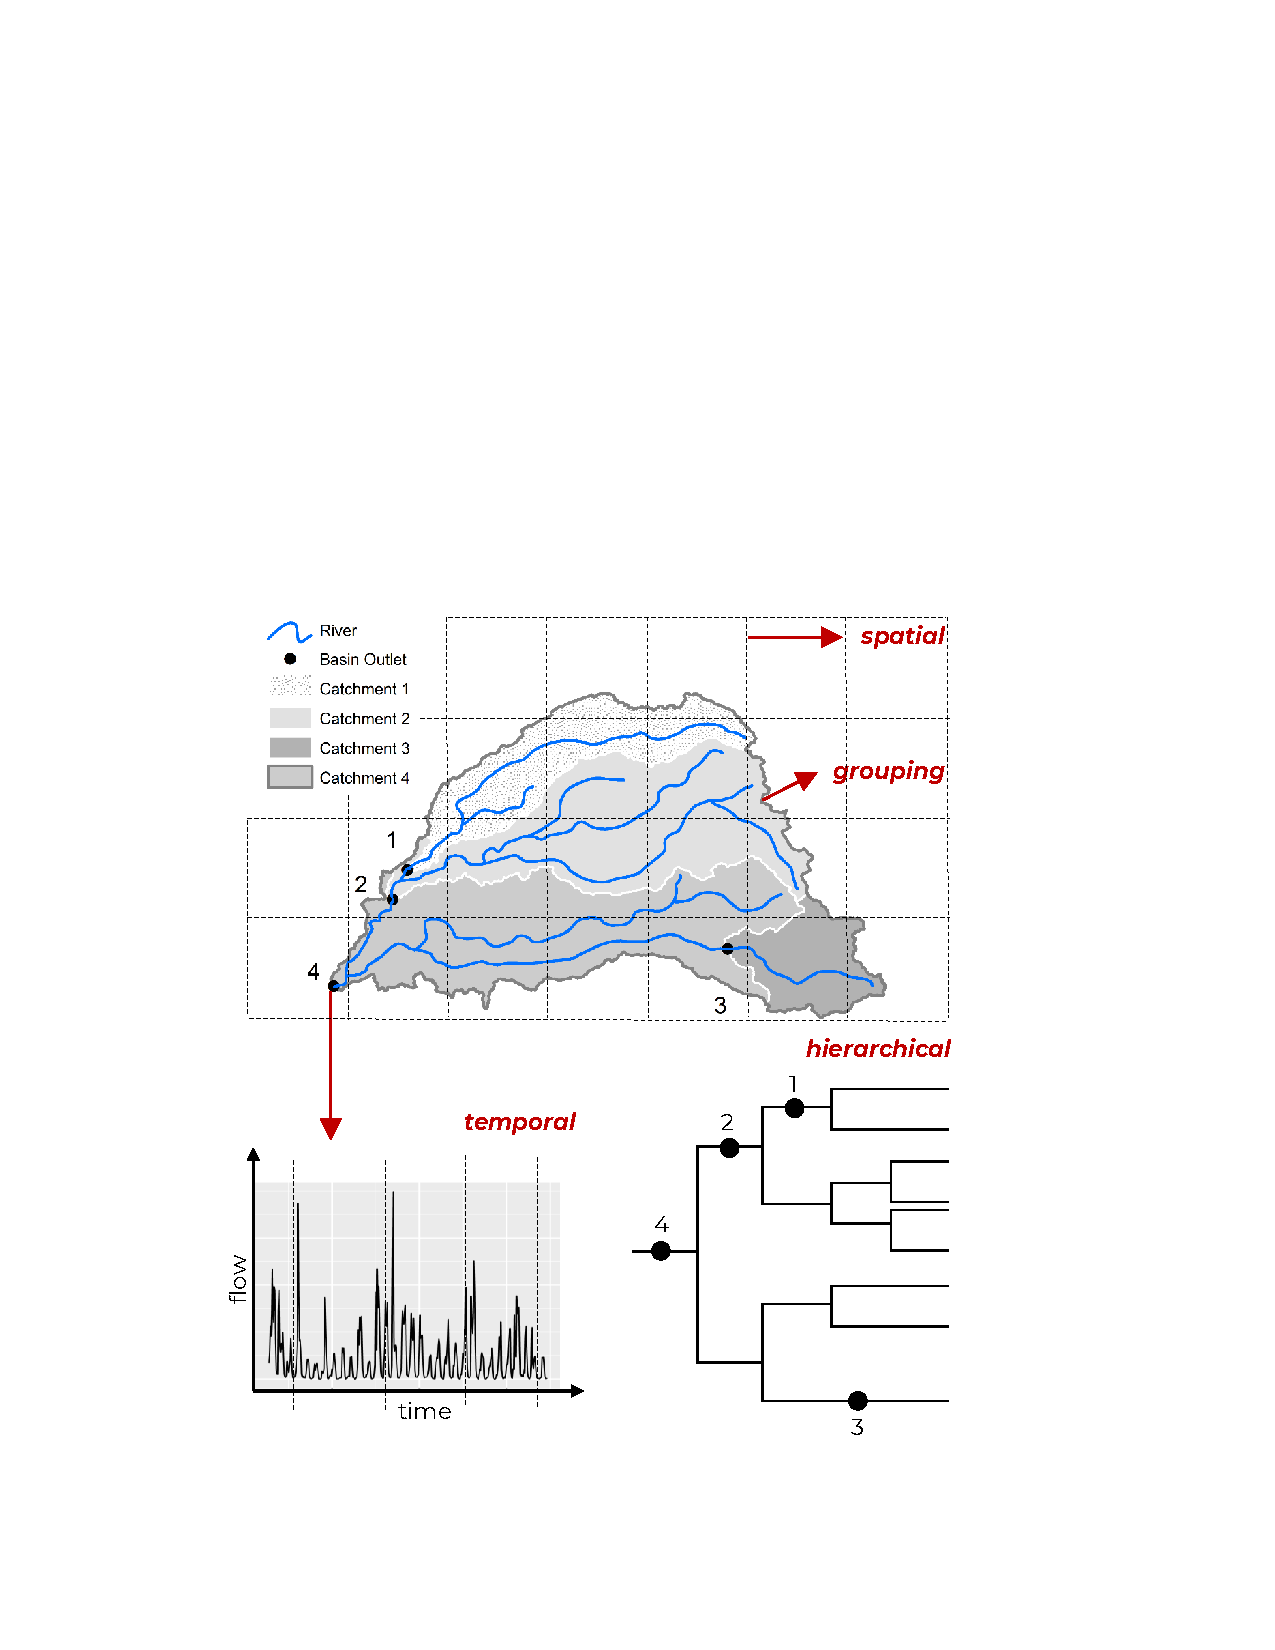
\includegraphics[width=18cm,trim={2cm 3.2cm 0 10.2cm},clip=true]{plots/structured.pdf}
	\caption{The four types of dependence structures in gauged data and blocking strategies} 
	\label{fig:structured}
\end{figure}

% the CV methods? INCLUDE BOOTSTRAP HERE TOO, AND BLOCKING BOOTSTRAP
In predictive modeling, the goal is to accurately predict data, with structures mentioned above, at unmeasured locations either in the past in locations not gauged, or in the future where observations do not yet exist. Therefore, the predictive accuracy of the \textit{training set}, the data the model is trained on, is of little consequence. The \textit{test set} error, the error of a set of data not seen by the model, is the true measure of model accuracy. 

Moreover, the predictive accuracy of the model on the training set can severely differ from the test set. With increasing model complexity (e.g., adding parameters to the model), clearly the model will fit the training data increasingly well. However, errors in the test set behave differently as is evident in the characteristic U-shape of the bias-variance tradeoff curve \cite{friedman2001elements}. The expected error in the test set is a polynomial of power two (See Equation \ref{eq:bvt}) and is comprised of variance, bias, and a constant term. In the first portion of the U, bias will decrease more than the gain in variance, however, past some point, we are now overfitting and the gain in variance is too much to be offset by the decrease in bias. Therefore, depending on how we specify the model, we will lie somewhere along this U shape and cannot substitute training error rates for the true predictive capability of the model. 

The test set error can be easily calculated if such a data set exists, or, it can be estimated by holding out a subset of the training data. The holding-out is achieved by resampling strategies, to effectively creating a test set. Two resampling methods are: \textit{cross-validation} and \textit{bootstrapping}. In cross-validation, the data set is split into testing and training data sets where each observational unit gets a chance at being in the test set once. In bootstrapping, sampling is done with replacement where each observational unit gets an equal chance at being selected and being selected more than once. In this case, on average 1/3\textsuperscript{rd} of the data set will end up not being selected at all, in other words these observations are out-of-bag \cite{efron1997improvements}. 

With the test set, that is held out observed data, and our model's results, we can conveniently apply any statistical measure of fit desired as a proxy for model accuracy (e.g., Nash-Sutcliffe Efficiency (NSE)). 

% the problem
Most studies, in water resources, ignore dependence structures in the data when devising a resampling strategy. When testing data are randomly selected from the entire spatial domain, training and testing data from nearby locations will be dependent due to \textit{spatial autocorrelation}. Therefore, if the objective is to project outside the spatial structure of the training data (e.g., to an ungauged basin), error estimates from random cross-validations or the bootstrap statistic, will be overly optimistic \cite{roberts2017cross}. 

% NOT RELEVANT HERE, MAKE A NEW CHAPTER MAYBE?
% Most studies, also fail to examine the autocorrelation of the errors produced by the developed models; as such, inferential results can be biased. Either including additional predictor variables, or choosing a different functional form has to be considered if a strong autocorrelation is detected in the model's residuals. The problem of inference cannot be diagnosed without explicitly checking for the spatial and temporal variability of the residuals, which are supposed to be independent and not correlated. A simple visual check or a formal test of the significance of Moran's I or Geary's C can help in this regard. 

In essence, a correlation structure points to a pseudo replication problem (See Figure \ref{fig:marbles}). For $x^d$ at a distance, $\Delta d$, from $x^{d+\Delta d}$, where $x^d$ and $x^{d+\Delta d}$ are autocorrelated. The distance $\Delta d$ can be defined in time, space, or hierarchy. In random resampling, either of the autocorrelated values may lie in the bag of samples given to the model, or it may be left out-of-bag. Therefore, the model can easily predict one, given that the other is likely in the bag. However, in blocking resampling the two observations are connected and will both end up in the bag or out-of-bag. Here, the model is forced to predict a phenomenon from other observations. 

\begin{figure}[ht]
	\centering
	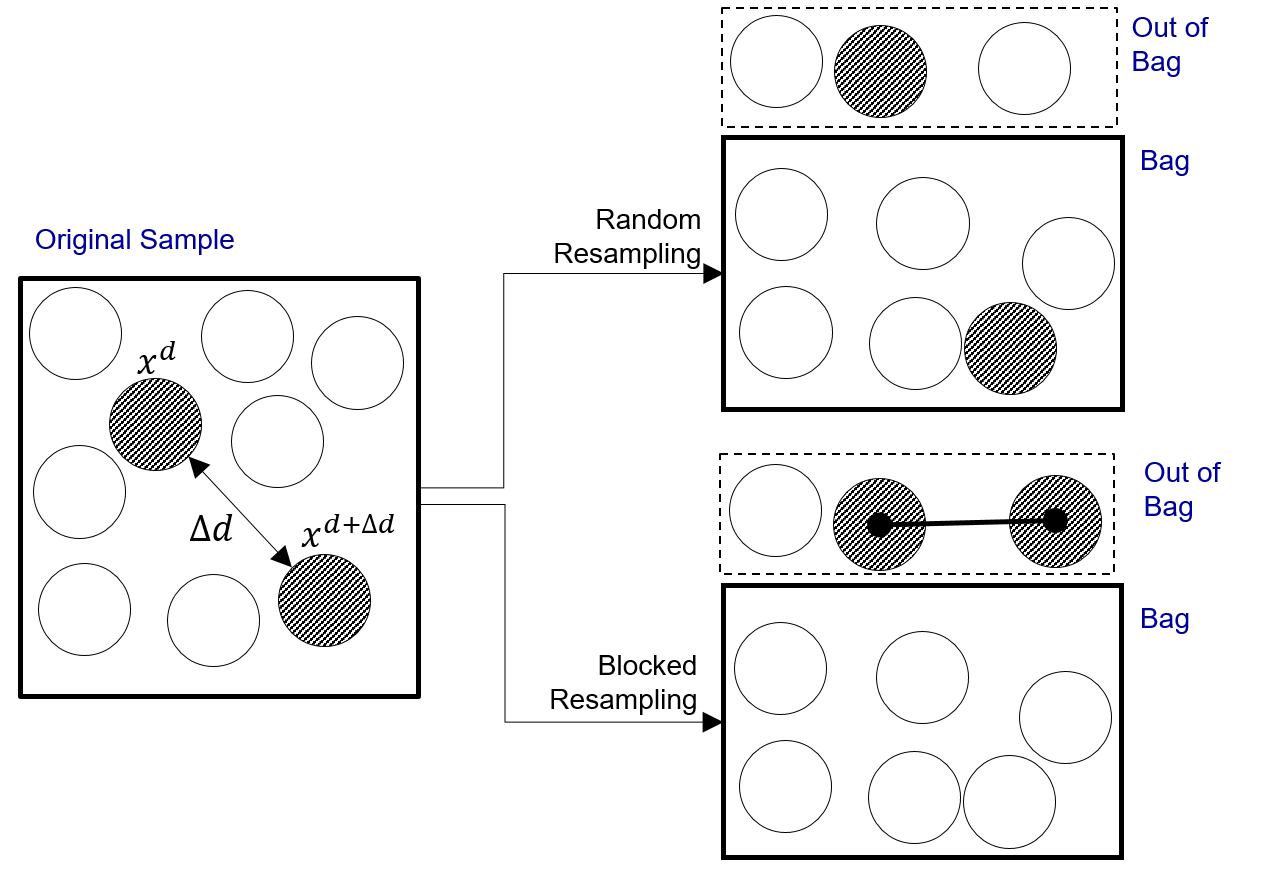
\includegraphics[width=15cm,trim={0 0 0 0},clip=true]{plots/resampling.png}
	\caption{Autocorrelation is a pseudo replication problem. The two grey marbles are autocorrelated. A model that uses random resampling will be able to easily predict one grey marble since it has seen the other. When blocking, the observations move in and out of the bag together.} 
	\label{fig:marbles}
\end{figure}

% Why bother? 
While correlation structures may not be as problematic in conventional statistics, combined with high-dimensions and low sample sizes, predictive methods suffer. Compounding the problem can be low computational abilities (See Figure \ref{fig:blocksizes}).

\begin{figure}
	\centering
	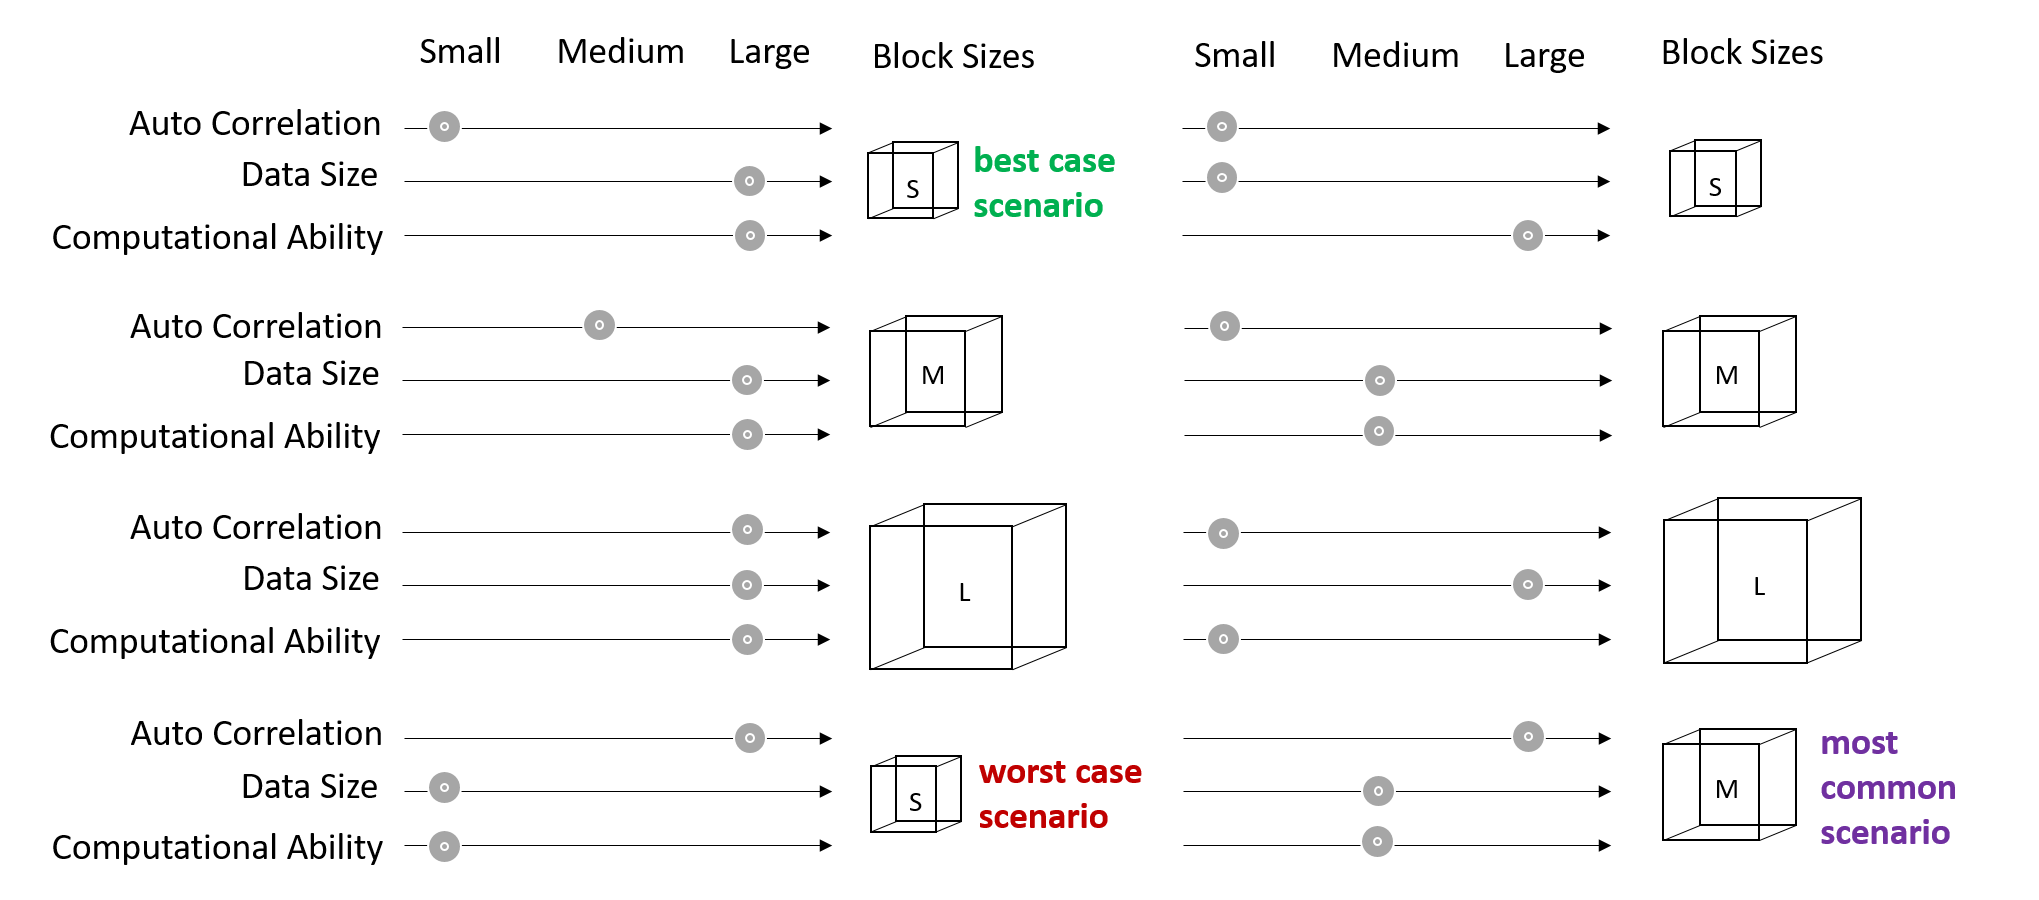
\includegraphics[width=15cm,trim={0 0 0 0},clip=true]{plots/blocksizes.png}
	\caption{The block size in resampling methods is a function of the autocorrelation, data size, and computational ability.} 
	\label{fig:blocksizes}
\end{figure}

%-----------------------------------------------------------------------------------------------------------------------------------------------------------------------------------------------------
\section{Research Design} \label{ch5:design}
Resampling methods are generally used to either: (1) estimate the accuracy of sample statistics (e.g., the standard deviation of an $\alpha$ parameter in a linear model $y=\alpha x+\beta$); (2) estimate the accuracy of significance tests (e.g., p-values); or (3) test the models. In hydrology, when examining observed data, the true population (i.e., the set of all possible hydrologic states) is unknown and the true error in the model or a sample statistic is unknowable. Therefore, we commonly use resampling methods to test our model's predictions. 
%In this case, our models will be performing quite differently from one another because of the differences in training and testing splitting strategies, which will be explained later. 
% To some extent, the modeling method follows that outlined in \cite{roberts2017cross}. 

In this study, data from a mechanistic simulation model, the Basin Characterization Model (BCM), with fitted values are considered as ``true" unimpaired flows. The BCM approximates California hydrology well. It estimates monthly unimpaired flows and is developed and maintained by the U.S. Geological Survey (USGS). The data spans California at 270m x 270m resolution. The recharge and runoff estimates from the BCM are attained from physically based equations that calculate potential evapotranspiration, snow, excess water, and actual evapotranspiration. Depending on soil properties and the permeability of underlying bedrock, surface water can be classified for each cell as either recharge or runoff \cite{flint2014california}. 

The recharge and runoff rasters can be aggregated to any given basin. Here, the machine learning model will be trained on the simulated runoff values from the BCM aggregated to the CDEC basins (See Figure \ref{fig:map}). The developed data set has approximately 18,500 monthly unimpaired flow observations in acre-feet (AF) (See appendix \ref{f:bcmdata} for more info). The data spans from 1895 to 2018 at a monthly time step. As mentioned in Chapter \ref{ch3:guide}, we will develop a GLM, RNN, and TMARS model. That said, the focus of this study is to demonstrate the differences between the cross-validation methods, not on the data or the machine learning method themselves; the purpose is to see which resampling strategy used in the machine learning algorithm gives the closest estimate to the true model error. That is, we want to see which cross-validation or bootstrap method is most appropriate for the machine learning model predicting values of a known model. In this chapter, we considered MSE as the loss function and the model measure of fit (See Equation \ref{eq:mse}).

To find the MSE of the machine learning technique: (1) simulate $n$ landscapes of the data by resampling the original data set using the bootstrap method (resampling with substitution); (2) separate the data into training and testing sets (use the CV or BS methods discussed below); (3) for each simulation feed the training data into the desired machine learning algorithm (i.e., a GLM, RNN and TMARS); (4) calculate the desired model measure of fit for each of the simulations; and (5) compare the Probability Density Function's (PDFs) of the model measures of fit with an ``ideal" one (See Figure \ref{fig:bsmethods} \&\ref{fig:cvmethods}).   

In both the cross-validation and bootstrap, the resampling results are compared to an ``ideal'' MSE, which was calculated by: (1) producing one model for each simulated landscape; (2) using said model to predict to the other $n-1$ landscapes; (3) using the predicted and observed values to calculate the MSE for each $n-1$ landscape; (4) averaging the MSE of the $n-1$ landscapes; (5) repeating the process for all $n$ landscapes; and (6) resulting in $n$ MSEs, one for each landscape, which can be plotted as a PDF (See Figure \ref{fig:idealmethod}). 

% can use a parametric bootstrap, but explain the high dimensionality of the problem
\begin{figure}[ht]
	\centering
	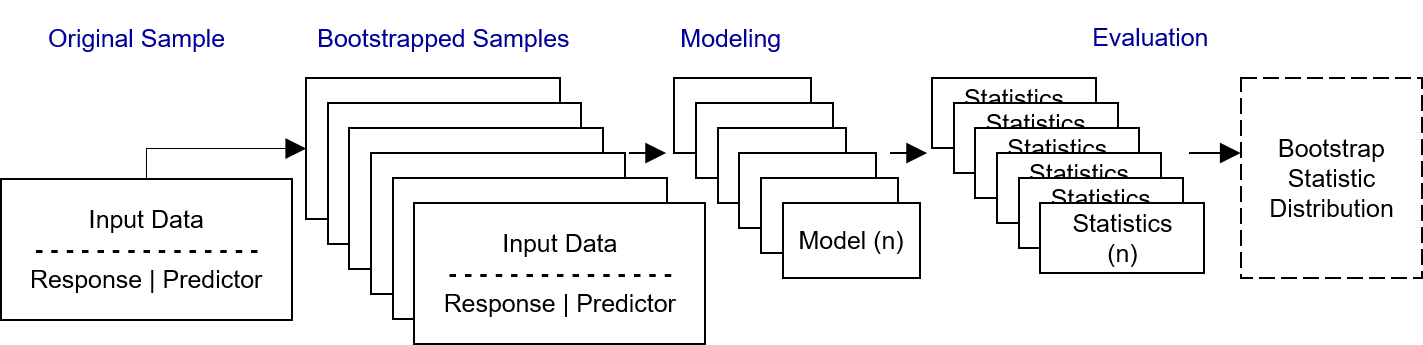
\includegraphics[width=15cm,trim={0 0 0 0},clip=true]{plots/bs_flowchart.png}
	\caption{Research design: We employ the bootstrap method to find the distribution of the bootstrap statistic.} 
	\label{fig:bsmethods}
\end{figure}

\begin{figure}[ht]
	\centering
	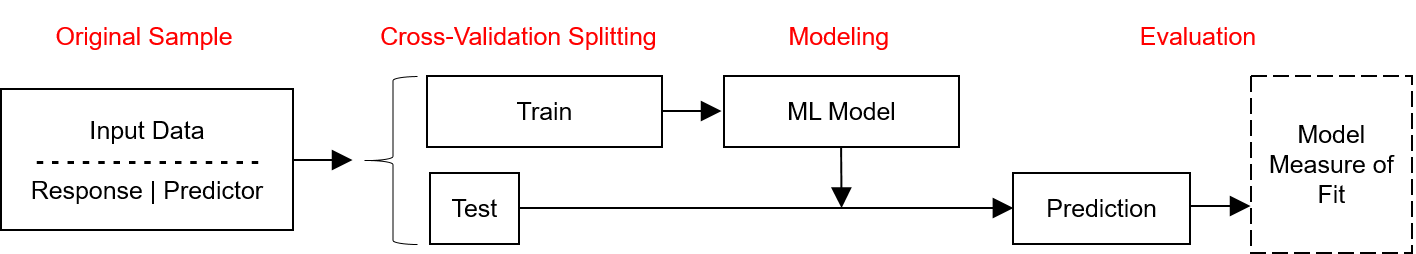
\includegraphics[width=15cm,trim={0 0 0 0},clip=true]{plots/cv_flowchart.png}
	\caption{Research design: We employ the cross-validation method to find the model error estimate.} 
	\label{fig:cvmethods}
\end{figure}

\begin{figure}[ht]
	\centering
	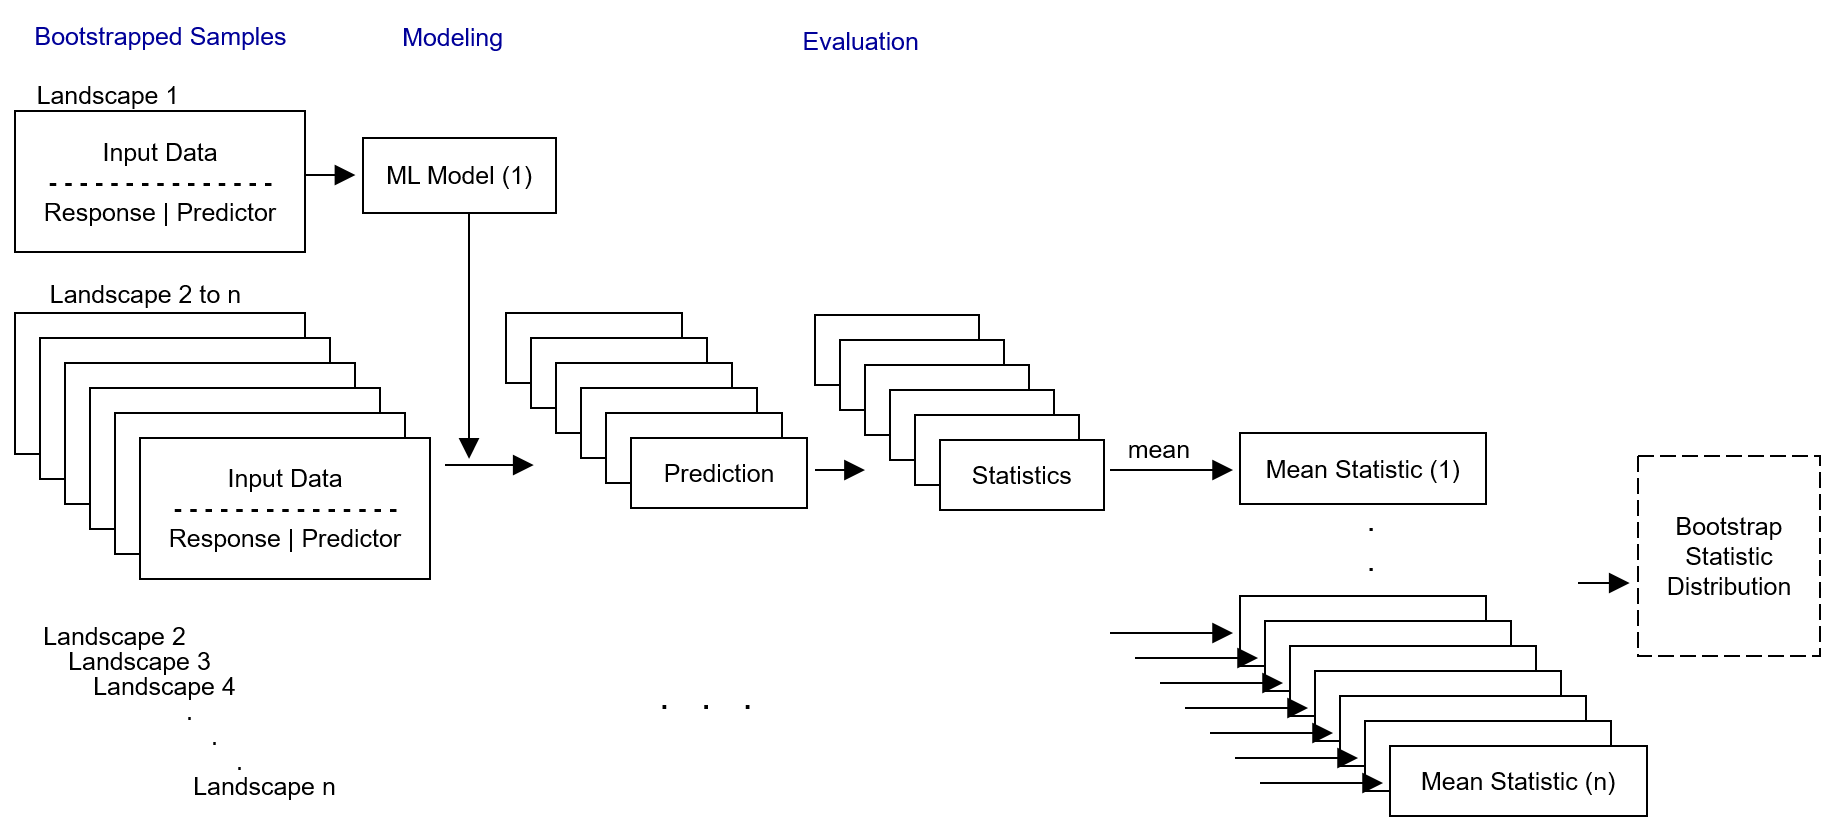
\includegraphics[width=15cm,trim={0 0 0 0},clip=true]{plots/ideal_flowchart.png}
	\caption{Research design: compare the errors with that of an ``ideal" model.} 
	\label{fig:idealmethod}
\end{figure}

%-----------------------------------------------------------------------------------------------
\subsubsection*{Resampling Methods} \label{ch5:resamp}
The second step in the methods mentioned above, separating the data in to training and testing sets, can be accomplished by one of the following methods: 

%---------------------------------------------
\textbf{Cross-Validation}
\begin{itemize}
	\item Resubstitution: the test set is the training set. Here, the model is evaluated against the same data it has already seen. We expect the model to perform the best here and the PDF of the residuals to be closest to 0. 
	\item Randomized or Monte-Carlo:cross-validation
		\subitem Validation Set: the test set is a random 1/2 of the full data set. the training set is the other 1/2. This method is run twice, once with the first half as a test set and next with the second half being the test set. 
		\subitem 5-Fold: the data is split into 5 folds. In each iteration each fold is considered the test set and the other 4 folds the training set. 
		\subitem 10-Fold: the data is split into 10 folds. In each iteration each fold is considered the test set and the other 9 folds the training set. 
	\item Leave One Out (LOO): in each iteration, one instance of the data is help out, and the rest of the data set is the training set. most intense computationally.
	\item Leave One Group Out (LOGO): in each iteration, one basin's data is held out as a whole and the rest of the basins become the training set. The process is repeated for each basin. 
	\item Leave Multiple Groups Out (LMGO): in each iteration, 1/5\textsuperscript{th} or 1/10\textsuperscript{th} of the basin's are held out and the rest of the basins become the training set. The process is repeated for each fold. 
	\item Leave Hierarchies Out (LHO): blocking is design across similar stream orders. %Because of the limitations imposed by datasize we have not considered this cross-validation strategy in this experiment. 
\end{itemize}

%------------------------------------------------
\textbf{Bootstrap Methods}
\begin{itemize}
	\item Resubstitution: same as above, the test set is the training set.
	\item Randomized or Monte-Carlo: the most popular form of bootstrapping where a new data set is built from randomly resampling the original sample with substitution. The length of the data set is the original length of the data set.
	\item Blocked By Group (BBG): the data set is blocked by unique basins. The basins are randomly resampled with substitution. Since the basins may have differing record lengths, the length of the data set may not match the original data set. However, the data set will have the same number of basins as in the original data set. 
	\item Blocked By Multiple Groups (BBMG): the data set is blocked by multiple basins. The grouped basins are randomly resampled with substitution. As the group sizes become larger the blocking size becomes larger. 
	\item Blocked By Hierarchy (BBH): the data set is blocked by stream order. The grouped basins are randomly resampled with substitution. Some stream orders have a chance of occurring in the data set twice where some are left out. 
\end{itemize}

%-----------------------------------------------------------------------------------------------------------------------------------------------------------------------------------------------------
%\section{Preliminary Results} \label{ch5:results}
%True and estimated test MSE for the simulated data sets. PDF of residuals. 
%
%Results show that ignoring the dependence structures when devising testing and training sets produces artificially low errors (See Figure \ref{fig:density}). Here, the resubstitution and randomly drawn folds show lower errors than the blocking methods LOGO and LMGO K-Fold. 
%
%\begin{figure}
%	\centering
%	\begin{subfigure}{.5\textwidth}
%  		\centering
% 		 \includegraphics[width=\textwidth, trim={0 0 0 0}, clip=true]{plots/Rplot22_density_ae.png}
%  		\caption{The error in unimpaired flow. Results are for one simulation. \\}
%  		\label{fig:errorpdf}
%	\end{subfigure}% 
%	\begin{subfigure}{.5\textwidth}
%  		\centering
%  		\includegraphics[width=\textwidth, trim={0 0 0 0}, clip=true]{plots/Rplot24_density.png}
%  		\caption{The model RMSEs for each cross-validation method. Results are across the 25 simulations.}
%  		\label{fig:rmsepdf}
%	\end{subfigure}
%	\caption{PDFs of model error.}
%	\label{fig:density}
%\end{figure}
%
%% Results also show that the size of the blocks matter. The validation set approach most accurately predicts the model error, then the Random 5-Fold, the Random10-Fold and the Resubstitution CV methods. Same phenomenon exists in grouping blocking method: the 5-Fold LOGO most accurately predicts the model error, then the 10-Fold LOGO, the LOGO method and the Resubstitution method. 
%
%\begin{figure}
%	\centering
%	\begin{subfigure}{.5\textwidth}
%  		\centering
% 		 \includegraphics[width=\textwidth, trim={0 0 0 0}, clip=true]{plots/Rplot20_r2map_wrong.png}
%  		\caption{Random 5-Fold CV.}
%  		\label{fig:random5fold}
%	\end{subfigure}% 
%	\begin{subfigure}{.5\textwidth}
%  		\centering
%  		\includegraphics[width=\textwidth, trim={0 0 0 0}, clip=true]{plots/Rplot20_r2map.png}
%  		\caption{LOGO CV.}
%  		\label{fig:logocv}
%	\end{subfigure}
%	\caption{Random 5-Fold CV gives deceptively high R\textsuperscript{2} model fit values.}
%	\label{fig:spatialcvperformance}
%\end{figure}
%
%% The spatial variability. Put the maps of Cali side by side. use the mean of the nsim RMSE values as the point. do this for resub, random 5 fold, and logo only. (See Figure \ref{fig:spatialcvperformance}). Shows we still haven't gotten rid of the spatial autocorrelation!

%-----------------------------------------------------------------------------------------------------------------------------------------------------------------------------------------------------
\section{Conclusion} \label{ch5:conclusion}
This chapter presents various blocking resampling techniques where the observations in a block are bonded together. The idea behind blocked resampling is simple: \textit{birds of a feather flock together}, or more accurately birds of a feather \textit{should} flock together. That is, if two observations are autocorrelated they should be both included in the bag, or training set, or both be out-of-bag, or in the test set. 

These blocking methods should show how much random methods underestimate the model error. That is, models evaluated with random methods may actually perform worse than we expect due to the pseudo-replication problem that autocorrelation presents. This isn't to say that, in hydrology, random resampling is never useful; the studies, in which a random test-train split is considered, are most appropriate for predicting flow for a sparsely incomplete gauge record, and the studies, in which holding out blocks of data in time is considered the resampling strategy, are most appropriate for predicting streamflow in time for that location. One should not expect to use these resampling strategies and get the same predictive accuracy in a purely ungauged basin problem, where blocks are supposed to be designed across geographic space (or hierarchical structure). 

This chapter proposes applying multiple resampling strategies to the ungauged basins problem and comparing the resultant PDFs to that of an ideal model. We can then visualize how far errors predicted with random resampling strategies are from the ideal scenario. 

% The journey was: we modeled, we estimated the error and did suspiciously well, we estimated the error again and got a more accurate estimate of the error, and then we found that our models aren't quite as good as we think. 

% However, appropriate resampling methods can account for structures in the data, and therefore, the test set can give a more accurate model error estimate. 

% A blocking cross-validation strategy, like the leave multiple groups out cross-validation (LMGO) method, is most appropriate for a study that intends to model the response variable in locations for which no data was observed. 

%Finally, resampling for model error estimation should follow these steps: \\
%(1) Does the data show dependence structures? Access the degree of dependence. \\
%(2) Determine modeling objective: i) to complete a sparsely missing record? ii) to predict in time in the past iii) to predict in space in the past iv) to predict into the future. \\
%(3) Design the cross-validation strategy depending on the modeling objective and the dependence structures identified. \\
%(4) Make one model for each fold. \\
%(5) Determine the suitability and applicability of the model. \\
%(6) Make final predictions using a full model. 





\chapter[Climate Change]{Climate Change and Future Unimpaired Flow} \label{ch5:climatechange}
\chaptermark{Climate Change}
\setlength{\epigraphwidth}{5.5in}
\epigraph{For all of its uncertainty we cannot flee the future.}{Barbara Jordan, \textit{``Democratic National Convention Keynote Address''}, 1976}

%----------------------------------------------------------------------------------------------------------------------------------------------------------------------------------------------------------
\section*{Summary}
Future water resources conditions are usually estimated using projected climate variables (i.e., precipitation and temperature) from global climate models (GCMs) and a hydrologic model that routes precipitation to runoff. \citeA{pierce2018climate} identify a subset of four, out of the 32, GCMs that have done particularly well reproducing California's historical climate and are recommended when using more GCM data is prohibitive. In this chapter, these models each with two RCPs (4.5 and 8.5), are used to study future hydrology. \citeA{pierce2018climate} bias-corrected and downscaled the GCM data using the Localized Constructed Analogues (LOCA) statistical method. The downscaled runoff was then aggregated to the CDEC basin boundaries as a simple routing technique for this dissertation. Each downscaled climate change model data is put through the NN model built on past hydrology and the model predictions are compared to the climate model projections. 

There is fairly good agreement in the statistical (NN) model's unimpaired flow predictions and the mechanistic (GCM) models' routed runoff (R\textsuperscript{2}= [0.65-0.72]). However, the NN model does not capture low flows like the climate models and overestimates their values so much that when we compare more smoothed data (with a moving average window) we can see a bias emerge (e.g., $\beta_1$= 0.95 to 1.84 for CanESM2 RCP 4.5). This can also be seen in the time series comparisons; with a larger moving average window, the NN model's predictions are consistently higher than the climate model projections. 

%----------------------------------------------------------------------------------------------------------------------------------------------------------------------------------------------------------
\section{Introduction}
Future water resources conditions are usually estimated using projected climate variables (i.e., precipitation and temperature) from global climate models (GCMs) and a hydrologic model that routes precipitation to runoff. A more robust climate assessment relies on multiple scenarios of future climate from current GCMs available. Two common Representative Concentration Pathways (RCPs) provide information on possible scenarios or development trajectories for the main forcing agents of climate change. RCPs encapsulate particular sets containing emission of aerosols, concentration of greenhouse gasses, and land-use trajectories. For example, RCP 4.5 is a ``medium'' stabilization emissions scenario that models a future where societies attempt to reduce greenhouse gas emissions, while RCP 8.5 is a very high baseline or ``business-as-usual'' emission scenario \cite{van2011representative}. 

The data used here originally came from the Climate Model Intercomparison Project version 5 (CMIP5; \citeNP{taylor2012overview}), which includes 32 coarse-resolution ($\sim$ 100 km) GCMs. The data were bias corrected and downscaled using the Localized Constructed Analogues (LOCA) statistical method to better capture key features in California's climate \cite{pierce2018climate}. These data are available at www.caladapt.org and can be downloaded with a simple {\tt Rcurl} script and the CalAdapt API. 

Differences in climate change projections from different climate models arises from: (1) model uncertainty: inexact and differing representation of various processes, (2) scenario uncertainty: unknown rates and changes in climate forcings (e.g., rate and concentration of CO\textsubscript{2} and other greenhouse gases), and (3) climate uncertainty: unknown  internal variability of the climate such as El Niño \cite{hawkins2011potential}. \citeA{pierce2018climate} identifies a subset of four, out of 32, GCMs that have done particularly well reproducing California's historical climate and are recommended when using more GCM data is prohibitive. In this chapter, the following models, each with two RCPs (4.5 and 8.5), are used to explore future hydrology:

\begin{itemize}
	\item CanESM2 (CCCma, BC, Canada): an ``average'' model in terms of changes in precipitation and temperature.
	\item CNRM\-CM5 (CNRM and CERFACS, Toulouse, France): a ``cool/wet'' model. %, but, is merely less warm/dry than others.
	\item HadGEM2\-ES (Met Office Hadley Centre, UK): a ``warm/dry'' model.
	\item MIROC5 (JAMSTEC, AORI, and NIES, Japan): a model most unlike the other three.
\end{itemize}

%----------------------------------------------------------------------------------------------------------------------------------------------------------------------------------------------------------
\section{Climate Change Data}
Figures \ref{fig:rpdmap_ppt}, \ref{fig:rpdmap_tmp}, and \ref{fig:rpdmap_rnf} compare the relative percent difference (RPD) in precipitation, temperature, and runoff in the different climate models. To calculate RDP, first, the annual values are averaged across time in both the projected data (2015-2099) and the observed data (1914-2014). Then, the RDP is calculated using Equation \ref{eq:rpd}. Its value always lies between $-200$\% and $200$\%. It is positive when the mean projected data exceeds the mean observed and negative when the mean observed exceeds the mean projected. A regular percent difference was not calculated because dividing by zeros in the mean observed values creates large relative errors. 

\begin{equation}
	\label{eq:rpd}
	RPD(x, y) =2 \frac{x-y}{|x|+|y|} *100\% \quad\quad\text{RPD} \in $[-200\% , 200\%]$\\
\end{equation}

%compared climate model predictions against one another
%Annual rolling mean and sd plots

%\begin{figure}
%	\centering
%	\includegraphics[width=\textwidth,trim={0 0 0 0},clip=true]{plots/.png}
%	\caption[]{} 
%	\label{fig:}
%\end{figure}

\begin{figure}
    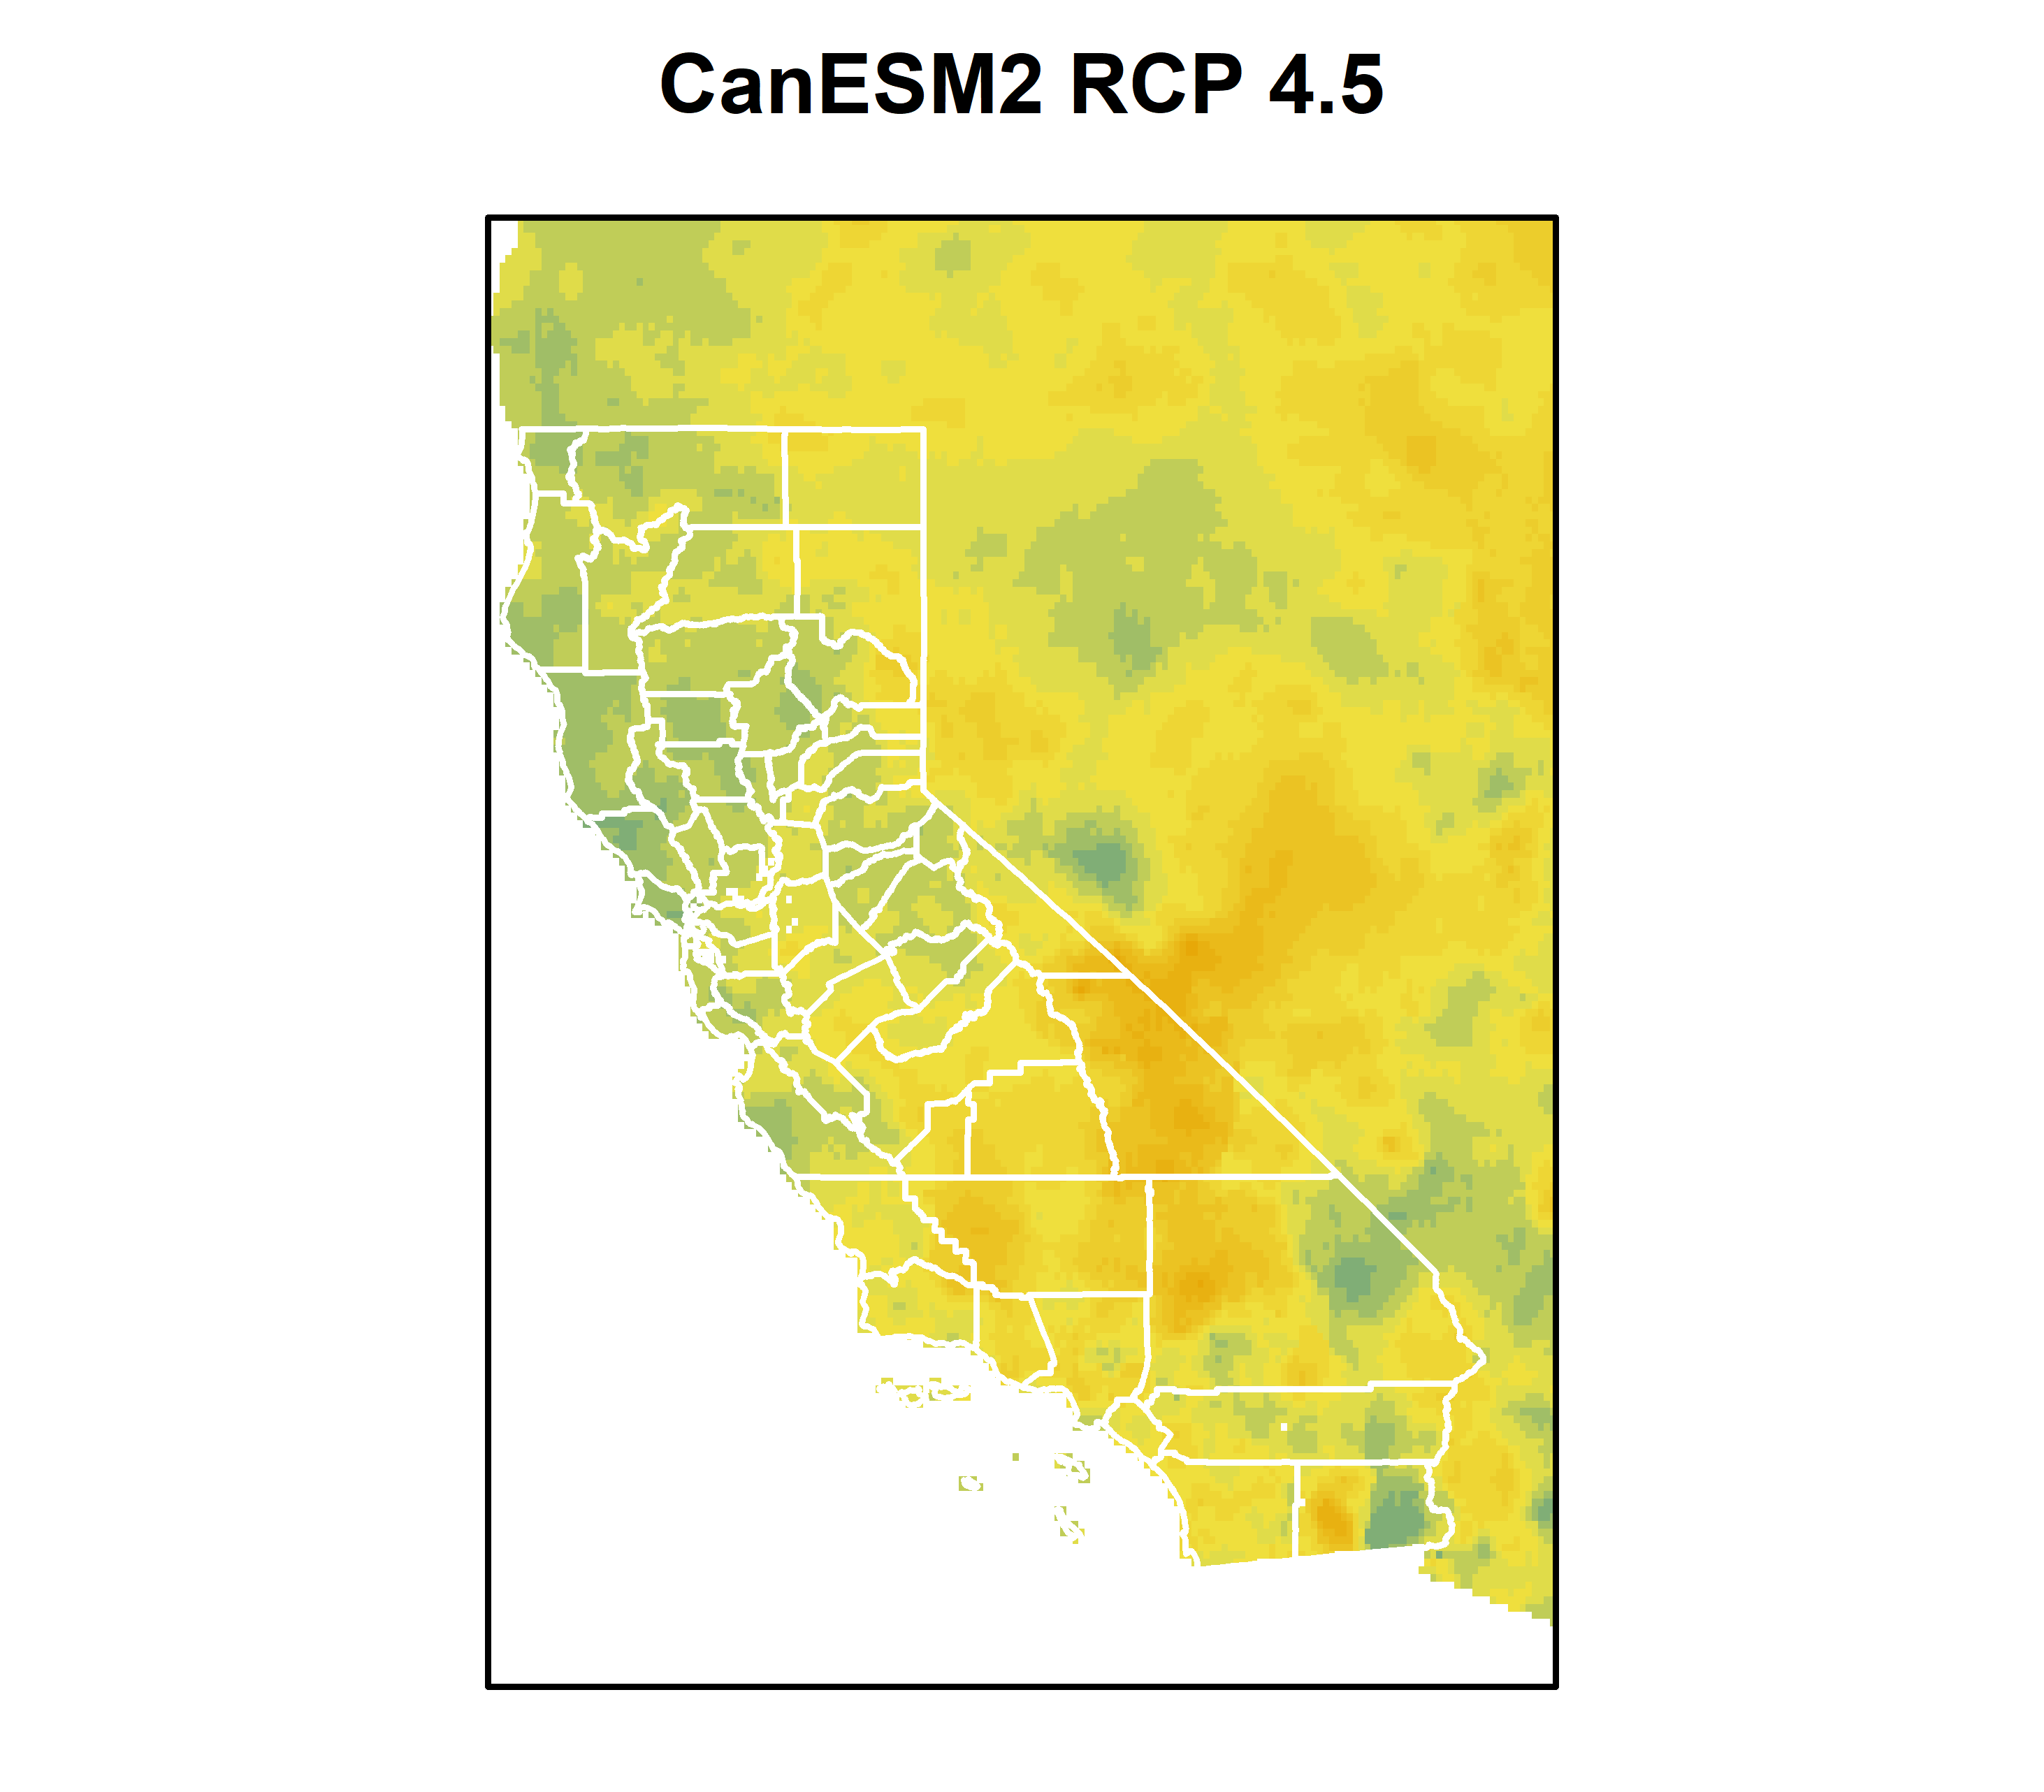
\includegraphics[width=.24\textwidth, trim={1cm 0 0 0}]{plots/rplot54_PPT_CanESM2_45_rpd.png}\hfill
    \includegraphics[width=.24\textwidth, trim={1cm 0 0 0}]{plots/rplot54_PPT_CanESM2_85_rpd.png}\hfill
    \includegraphics[width=.24\textwidth, trim={1cm 0 0 0}]{plots/rplot54_PPT_CNRMCM5_45_rpd.png}\hfill
    \includegraphics[width=.24\textwidth, trim={1cm 0 0 0}]{plots/rplot54_PPT_CNRMCM5_85_rpd.png}
    \includegraphics[width=.24\textwidth, trim={1cm 0 0 0}]{plots/rplot54_PPT_HadGEM2ES_45_rpd.png}\hfill
    \includegraphics[width=.24\textwidth, trim={1cm 0 0 0}]{plots/rplot54_PPT_HadGEM2ES_85_rpd.png}\hfill
    \includegraphics[width=.24\textwidth, trim={1cm 0 0 0}]{plots/rplot54_PPT_MIROC5_45_rpd.png}\hfill
    \includegraphics[width=.24\textwidth, trim={1cm 0 0 0}]{plots/rplot54_PPT_MIROC5_85_rpd.png}
    \caption[Relative percent difference in precipitation for each climate model.]{Relative percent difference in precipitation for each climate model. MIROC5 RCP 8.5 and CanESM2 RCP 4.5 show the most amount of dryness across California. In other models, southern California becomes wetter (e.g, CNRMCM5 RCP 4.5 and HadGEM2ES 4.5). This projected wetness can be viewed as a southward shift in the cooler/wetter climates of today. In all models, except for CanESM2, the RCP 8.5 scenario is dryer than its counter part RCP 4.5. }
    \label{fig:rpdmap_ppt}
\end{figure}

\begin{figure}
    \includegraphics[width=.24\textwidth, trim={1cm 0 0 0}]{plots/rplot54_TMP_CanESM2_45_rpd.png}\hfill
    \includegraphics[width=.24\textwidth, trim={1cm 0 0 0}]{plots/rplot54_TMP_CanESM2_85_rpd.png}\hfill
    \includegraphics[width=.24\textwidth, trim={1cm 0 0 0}]{plots/rplot54_TMP_CNRMCM5_45_rpd.png}\hfill
    \includegraphics[width=.24\textwidth, trim={1cm 0 0 0}]{plots/rplot54_TMP_CNRMCM5_85_rpd.png}
    \includegraphics[width=.24\textwidth, trim={1cm 0 0 0}]{plots/rplot54_TMP_HadGEM2ES_45_rpd.png}\hfill
    \includegraphics[width=.24\textwidth, trim={1cm 0 0 0}]{plots/rplot54_TMP_HadGEM2ES_85_rpd.png}\hfill
    \includegraphics[width=.24\textwidth, trim={1cm 0 0 0}]{plots/rplot54_TMP_MIROC5_45_rpd.png}\hfill
    \includegraphics[width=.24\textwidth, trim={1cm 0 0 0}]{plots/rplot54_TMP_MIROC5_85_rpd.png}
    \caption[Relative percent difference in air temperature for each climate model.]{Relative percent difference in air temperature for each climate model. In all models, California becomes hotter in all areas of the state; the relative percent difference is never negative. The Sierra-Nevada range and the northern part of California are projected to experience the brunt of the warming and the central valley and southern California are projected warm to a lesser extent. In all models, the RCP 8.5 scenario is slightly hotter than its counterpart RCP 4.5. Overall, there is more agreement between the models on air temperature changes than there is with precipitation.}
    \label{fig:rpdmap_tmp}
\end{figure}

\begin{figure}
    \includegraphics[width=.24\textwidth, trim={1cm 0 0 0}]{plots/rplot54_RNF_CanESM2_45_rpd.png}\hfill
    \includegraphics[width=.24\textwidth, trim={1cm 0 0 0}]{plots/rplot54_RNF_CanESM2_85_rpd.png}\hfill
    \includegraphics[width=.24\textwidth, trim={1cm 0 0 0}]{plots/rplot54_RNF_CNRMCM5_45_rpd.png}\hfill
    \includegraphics[width=.24\textwidth, trim={1cm 0 0 0}]{plots/rplot54_RNF_CNRMCM5_85_rpd.png}
    \includegraphics[width=.24\textwidth, trim={1cm 0 0 0}]{plots/rplot54_RNF_HadGEM2ES_45_rpd.png}\hfill
    \includegraphics[width=.24\textwidth, trim={1cm 0 0 0}]{plots/rplot54_RNF_HadGEM2ES_85_rpd.png}\hfill
    \includegraphics[width=.24\textwidth, trim={1cm 0 0 0}]{plots/rplot54_RNF_MIROC5_45_rpd.png}\hfill
    \includegraphics[width=.24\textwidth, trim={1cm 0 0 0}]{plots/rplot54_RNF_MIROC5_85_rpd.png}
    \caption[Relative percent difference in runoff for each climate model.]{Relative percent difference in runoff for each climate model. Much like the changes in precipitation, southern California becomes wetter in CNRMCM5 RCP 4.5 and HadGEM2ES 4.5, and in all models, except for CanESM2, the RCP 8.5 scenario is dryer than its counter part RCP 4.5. MIROC5 RCP 4.5 is most unlike the other models in that it projects a wetter environment for the majority of California (i.e., the central valley and southern California). However, its RCP 8.5 projects a much drier state.}
    \label{fig:rpdmap_rnf}
\end{figure}

Figure \ref{fig:rpd_var} compares the mean RPD in precipitation, temperature, and runoff for different GCMs. These values were calculated by: taking a 30 year subset of the annual values for the projected data (2070-2099) and the observed (1976-2005); finding the RDP for each year (with 1-to-1 matching: 2070 with 1976, 2071 with 1977, etc.); cropping these rasters to the California boundary; averaging the RDPs for each pixel across time; and averaging across space to arrive at one mean RDP for each GCM and RCP combination. Figure \ref{fig:rpd_var}(a) shows that models with RCP 8.5, on average, project hotter climates. The CanESM models and the CNRMCM5 RCP 8.5, on average, project wetter climates. Using these models can give us a wide range of possible futures (dry/wet, and warm/less warm) for California. Figure \ref{fig:rpd_var}(b) shows that runoff in all models generally increases linearly with precipitation and at a higher rate, confirming the positive relationship used when constructing runoff. 
 
\begin{figure}
	\centering
	\includegraphics[width=\textwidth,trim={0 0 0 0},clip=true]{plots/rplot56_relperdiff_all.png}
	\caption[Relative percent difference in precipitation, temperature, and runoff for different GCMs.]{Relative percent difference in precipitation, temperature, and runoff for different GCMs. (a) Models with RCP 8.5, on average, project hotter climates. The CanESM models and the CNRMCM5 RCP 8.5, on average, project wetter climates. (b) Runoff in all models generally increases linearly with precipitation and at a higher rate.}
	\label{fig:rpd_var}
\end{figure}

Figure \ref{fig:obscc_var} shows the mean annual precipitation, temperature, and runoff over time. These values were calculated by averaging the parameter value across California and Nevada for each year. With uncertainty in models, scenarios, and climate there are many varied projection paths these variables can take. MIROC 5 RCP 4.5 and CNRMCM5 RCP 4.5 project a wetter climate (confirming mapped values in Figure \ref{fig:rpdmap_rnf}). Annual temperature values slightly increase over time in all models with RCP 4.5 values generally lower than RCP 8.5.  Runoff shows more of a change compared to precipitation, with more frequent peaks in the projections compared to the observed. 

\begin{figure}
	\centering
	\includegraphics[width=\textwidth, trim={0 0 0 0}, clip=true]{plots/rplot55_obscc_all.png}
	\caption[Time series of projections in precipitation, temperature, and runoff.]{Time series of projections in precipitation, temperature, and runoff. MIROC 5 RCP 4.5 and CNRMCM5 RCP 4.5 project a wetter climate. Annual temperature values slightly increase over time in all models with RCP 4.5 values generally lower than RCP 8.5. Runoff seems to show more of a change compared to precipitation, with more frequent higher values in the projections compared to the observed.}
	\label{fig:obscc_var}
\end{figure}

To smooth out Figure \ref{fig:obscc_var}, Figures \ref{fig:rollmean_var} and \ref{fig:rollsd_var} show the rolling 10 year mean and standard deviations in annual precipitation, temperature, and runoff. These values were calculated by: first, taking a 10 year rolling window starting from 2015 and looking forward in time; finding the average or the standard deviation of the annual parameter values for each raster pixel in time with the last 10 years (2090-2099) discarded from the analysis; finding the spatial mean of the 10 year rolling mean or standard deviation for each parameter. Figure \ref{fig:rollmean_var} shows mean precipitation increasing in CNRMCM5 RCP 8.5. Mean temperature increases in most models and is more pronounced in RCP 8.5. Mean runoff follows mean precipitation trends. Figure \ref{fig:rollsd_var} shows standard deviations in precipitation increasing in CNRMCM5 RCP 8.5 and HadGEM2ES RCP 8.5. Standard deviation in temperature increase in MIROC5 RCP 4.5 and CNRMCM5 RCP 4.5. Standard deviations in runoff follows the trends seen in precipitation. In all but CNRMCM5 RCP 8.5 (cool/wet model), the differences in precipitation and runoff across models are evident from the beginning of the time period and the mean and standard deviations remain stationary. 

\begin{figure}
	\centering
	\includegraphics[width=\textwidth, trim={0 0 0 0}, clip=true]{plots/rplot57_rollmean_all.png}
	\caption[Time series of 10 year rolling mean in precipitation, temperature, and runoff.]{Time series of 10 year rolling mean in precipitation, temperature, and runoff. Most differences in precipitation between models is in the mean precipitation rather than in trends, except in CNRMCM5 RCP8.5 (cool/wet model). Mean temperature increases in most models and is more pronounced in RCP 8.5. Mean runoff follows the trends seen in mean precipitation.}
	\label{fig:rollmean_var}
\end{figure}

\begin{figure}
	\centering
	\includegraphics[width=\textwidth, trim={0 0 0 0}, clip=true]{plots/rplot57_rollsd_all.png}
	\caption[Time series of 10 year rolling standard deviation in precipitation, temperature, and runoff.]{Time series of 10 year rolling standard deviation in precipitation, temperature, and runoff. Standard deviations in precipitation increase in CNRMCM5 RCP 8.5 (cool/wet model) and HadGEM2ES RCP 8.5 (the warm/dry model). Standard deviation in temperature increase in MIROC5 RCP 4.5 and CNRMCM5 RCP 4.5. In RCP 4.5, the standard deviations decrease at the end of the century. Again, standard deviations in runoff follows trends seen in precipitation.}
	\label{fig:rollsd_var}
\end{figure}

%-----------------------------------------------------------------------------------------------------------------------------------------------------------------------------------------------------
\section{Methods}
Each downscaled climate change model data is put through the NN model built on past hydrology and the model predictions are compared to the climate model projections. The climate model projections come in raster (i.e., not routed) format. A simple aggregation to basin boundaries finds the mean precipitation (and its lagged values), mean temperature (and its lagged values), mean snow, and total runoff over the basin. One problem with this simple routing technique is that some end-of-month storms may end up as streamflow in the next month; some precipitation values are getting counted in the month that the flows it generates is not. Since, the model is on a monthly time-step we will ignore this small accounting difficulty. The other option was to use the Variable Infiltration Capacity (VIC) routed streamflows that do account for basin lags, however, this dataset was only developed for 11 basins, hand selected for the CALSIM II model's major reservoir inflow locations. To keep all our 67 diverse basins in the study we will use the aforementioned aggregation method as a good approximation for routing. 
 
%-----------------------------------------------------------------------------------------------------------------------------------------------------------------------------------------------------
\section{Results}
Figure \ref{fig:modcomp} shows the NN model predictions compared to climate model projections for unaggregated monthly data for each basin. There is fairly good agreement between the purely statistical (NN) and the mechanistic models (GCMs) with the highest R\textsuperscript{2} of 0.72 belonging to the CanESM2 and CNRMCM5 models. In all models the NN is slightly biased to predict higher values compared to the climate change models as is evident in the slope of the best fit line ($\beta_1>1$). 

\begin{figure}
	\centering
	\includegraphics[width=\textwidth,trim={0 0 0 0},clip=true]{plots/rplot52_obsvspred.png}
	\caption[NN model predictions compared to climate model projections.]{NN model predictions compared to climate model projections (monthly data for each basin). There is fairly good agreement between the purely statistical (the NN) and the mechanistic models (the climate change models) with the highest R\textsuperscript{2} being 0.72 for the CanESM2 and CNRMCM5 RCP 4.5 models.} 
	\label{fig:modcomp}
\end{figure}

Figure \ref{fig:density} shows the probability densities for the monthly NN unimpaired flow predictions and the climate model runoff projections. Similar to results in previous chapters, the NN model predicts fewer low flows compared to the runoff from climate models. There is very little difference in the densities across the various climate data in either the NN model prediction or runoff projections from the climate models themselves. Also, there is very little difference observed across the two RCPs. This shows that our simple routing precipitation to runoff eliminates the differences across models and should be replaced with a better model (e.g., VIC). 

\begin{figure}
	\centering
	\includegraphics[width=\textwidth,trim={0 0 0 0},clip=true]{plots/rplot53_density.png}
	\caption[Predicted unimpaired flow density compared to runoff densities from GCMs.]{Predicted unimpaired flow density compared to runoff densities from GCMs. The NN model does not capture low flows like climate models. There is very little difference in the densities across the various climate data in either the NN model prediction or runoff projections from the climate models themselves. Also, there is very little difference observed across the two RCPs.} 
	\label{fig:density}
\end{figure}

Figures \ref{fig:camean_monthly_comp}, \ref{fig:camean_annual_comp}, and \ref{fig:camean_10yr_comp} compare the monthly, moving 1 year average, and moving 10 year average NN model predictions with climate model runoff projection. Instead of showing each basin separately, this plot shows the mean flows across the 67 basins. The moving window allows us to view larger trends. Unsurprisingly, as the window grows larger, the values are ``smoothed out'', and the agreement (in terms of R\textsuperscript{2}) increases. For example, in the CNRMCM5 RCP 4.5 R\textsuperscript{2} increases from 0.77, to 0.90, and 0.96 when comparing monthly, moving 1 year average, and moving 10 year average values. However, with the increase in R\textsuperscript{2} the NN model biases increase as well. For example, the slope of the best fit line in CNRMCM5 RCP 4.5 increases from 0.95 to 1.44 and 1.74. This is due to the NN model's inability to capture a higher density at the lower flows, which was observed in Figure \ref{fig:density}.

\begin{figure}
	\centering
	\includegraphics[width=\textwidth,trim={0 0 0 0},clip=true]{plots/rplot58_camean_monthly_comp2.png}
	\caption[Mean California unimpaired flow NN model predictions vs. climate model projections (monthly data).]{Mean California unimpaired flow NN model predictions vs. climate model projections (monthly data). There is fairly good agreement between the two types of models on the average California flows. Compared to unaggregated monthly data model agreement slightly increases as the data gets aggregated across California.} 
	\label{fig:camean_monthly_comp}
\end{figure}

\begin{figure}
	\centering
	\includegraphics[width=\textwidth,trim={0 0 0 0},clip=true]{plots/rplot58_camean_annualrolling_comp2.png}
	\caption[Mean California unimpaired flow NN model predictions vs. climate model projections (annual moving average data).]{Mean California unimpaired flow NN model predictions vs. climate model projections (annual moving average data). There is fairly good agreement between the two types of models on the average California flows. Compared to monthly data, here, model agreement increases slightly.} 
	\label{fig:camean_annual_comp}
\end{figure}

\begin{figure}
	\centering
	\includegraphics[width=\textwidth,trim={0 0 0 0},clip=true]{plots/rplot58_camean_10yr_rolling_comp2.png}
	\caption[Mean California unimpaired flow NN model predictions vs. climate model projections (10 year moving average data).]{Mean California unimpaired flow NN model predictions vs. climate model projections (10 year moving average data). There is fairly good agreement between the two types of models on the average California flows. Compared to 1 year moving average data, here, model agreement increases slightly but so does biases (slope of the best fit line).} 
	\label{fig:camean_10yr_comp}
\end{figure}

Figures \ref{fig:camean_monthly_comp_ts}, \ref{fig:camean_annual_comp_ts}, and \ref{fig:camean_10yr_comp_ts} confirm the NN model's bias observed in the previous plots. Here, the monthly, moving 1 year average, and moving 10 year average NN model predictions and climate model runoff projections are plotted through time. As the window grows larger the NN model predictions increase as compared to the climate model predictions. This is again due to the NN model's inability to capture a higher density at the lower flows, which was observed in Figure \ref{fig:density}.

\begin{figure}
	\centering
	\includegraphics[width=\textwidth,trim={0 0 0 0},clip=true]{plots/rplot58_camean_monthly_comp.png}
	\caption[Mean California unimpaired flow climate model and NN model comparisons in time (monthly data).]{Mean California unimpaired flow climate model and NN model comparisons in time. The NN model captures the high flow events at the right time but is slightly under predicting them compared to the climate model projections.} 
	\label{fig:camean_monthly_comp_ts}
\end{figure}

\begin{figure}
	\centering
	\includegraphics[width=\textwidth,trim={0 0 0 0},clip=true]{plots/rplot58_camean_annualrolling_comp.png}
	\caption[Mean California unimpaired flow climate model and NN model comparisons in time (annual moving average data).]{Mean California unimpaired flow climate model and NN model comparisons in time (1 year moving average data). The NN model's predictions over-take the climate model projections.} 
	\label{fig:camean_annual_comp_ts}
\end{figure}

\begin{figure}
	\centering
	\includegraphics[width=\textwidth,trim={0 0 0 0},clip=true]{plots/rplot58_camean_10yr_rolling_comp.png}
	\caption[Mean California unimpaired flow climate model and NN model comparisons in time (10 year moving average data).]{Mean California unimpaired flow climate model and NN model comparisons in time (10 year moving average data).The NN model's predictions over-take the climate model projections and a larger moving window means larger differences.} 
	\label{fig:camean_10yr_comp_ts}
\end{figure}

%-----------------------------------------------------------------------------------------------------------------------------------------------------------------------------------------------------
\section{Conclusion}
This chapter used four global climate models with two RCPs each to estimate future hydrology. The climate variable from these models give a wide range of possible futures for California. Some models like the MIROC5 RCP 4.5 and CNRMCM5 RCP 4.5 project a wetter California while most other models project a drier climate in terms of precipitation. Most models agree that in both RCPs, temperatures will rise and are projected to increase 2-4 $^{\circ}$C for RCP 4.5 and 4-7 $^{\circ}$C for RCP 8.5 \cite{pierce2018climate}. Runoff projections show more floods compared to historical hydrology, but are stationary in their mean and standard deviations in all but one model (CNRMCM5, the cool/wet model). 

Statistical models operate from no apriori knowledge of hydrologic processes, and have to be used with caution when extrapolating beyond the time range they were trained on. There is fairly good agreement in the statistical (NN) model's unimpaired flow predictions and the mechanistic (GCM) model's routed runoff (R\textsuperscript{2}= [0.64-0.72]). However, the NN model does not capture low flows like the climate models and overestimates their values so much so that when we compare more smoothed data (with a moving average window) we can see a bias emerge ($\beta_1$= [0.95-1.84] for CanESM2 RCP 4.5 for example). This can also be seen in the time series comparisons, where with a larger moving average window the NN model's predictions are systematically higher than the climate model projections. 

Both the GCM or NN model projections are untestable, since the ``reality'' we need to test against will be available either too late or never-an unavoidable feature of all hydrological simulation models discussed by \citeA{klemevs1986operational}. We can argue that the GCM model's projections are slightly more reliable since the processes of finding the amount of recharge and runoff for each pixel ($\sim$ 100 km) from precipitation is grounded in hydrology. However, the downscaling to a finer resolution was a statistical process (i.e., LOCA downscaling), and the routing scheme used here was a simple statistical aggregation to basin boundaries. Therefore, even in the GCM projections many approximations are used to arrive at water balance estimates. The advantages of using statistical learning models still remain; they are easier to use, apply, and operationalize. The next chapter will explain some improvement strategies for the NN model. 

%\chapter[Beyond McDonaldization]{Beyond McDonaldization: The ``Robotanization" of Agriculture} \label{ch6:sociology}
\chaptermark{Beyond McDonaldization}
\setlength{\epigraphwidth}{4.5in}
\epigraph{The world is stranger than we can imagine and surprises are inevitable in science. Thus we found, for example, that pesticides increase pests, antibiotics can create pathogens, agricultural development creates hunger, and flood control leads to flooding. But some of these surprises could have been avoided if the problems had been posed big enough to accommodate solutions in the context of the whole.}{Richard Levins, \textit{``n.a.''}, 1995}

%------------------------------------------------------------------------------------------------------------------------------------------------------------------------------------------------------
\section*{Summary} 
Given the increasingly popular statistical learning methods and their resampling techniques, the sociological effects of these methods become important fro for both scholarship and application. In 2013, Monsanto paid \$930 Million USD to acquire The Climate Corporation \cite{frobes2013merger}. Monsanto is a large publicly traded agricultural multinational corporation, and The Climate Corporation is a digital agriculture company that examines field data. In other words, ``big-farma" has learned the potential of big data. Recent technological advances in big data is impacting the nature of agricultural (i.e., arable, livestock, horticulture, and fishery farming) work in various and complex ways. 

This chapter will explore the impacts of big data (BD), machine learning (ML), and artificial intelligence (AI) on arable farming and studies of farming. BD refers to data sets that are too large or complex for traditional data-processing application software to adequately deal with \cite{wiki2018bigdata}. ML is the development of computer programs that analyzes data and automatically learns and improves from experience without being explicitly programmed \cite{koza1996automated}.  ML is an application in the larger field of AI. BD, ML, and/or AI in farming, hereinafter referred to as ``robotany", manifest as a combination of data-heavy decision making and precision agriculture. 

Part of my research will be preparing a literature review on historical and recent mechanization trends in agriculture (e.g., the tomato harvester saving the California tomato) and the sociological process of McDonaldization. My research will cover these topics in the Science and Technology Studies discipline and the Cybernetics sub-discipline.

%-----------------------------------------------------------------------------------------------------------------------------------------------------------------------------------------------------
\section{Introduction} 
The major influences in the development of the first tomato picking harvester (See Figure \ref{fig:tomatoharvester}) were technologies such as, effective machines, specially bred tomatoes, careful irrigation and fertilization, and particular planting techniques, another major influence was a societal phenomenon: the fear of a lack of labor to handle the tomato crop, as the Brarcero migrant-worker program had ended \cite{rasmussen1968advances}. 

The two major hurdles to developing a mechanical tomato picker were the susceptibility of the tomato to bruising, thus making it a tough candidate for machine harvesting, and the fact that tomatoes did not all ripen at the same time, that is, they usually required multiple passes through the field. In the 1940s, UC Davis researchers successfully removed both obstacles; they developed a pear-shaped tomato particularly adapted to machine harvesting that would also ripen around the same time \cite{rasmussen1968advances}. Uniformity in shape and ripening time, brings the predictability needed for mechanization. Predictability is one aspect of McDonaldization. 

% For a brief history of farming (where we were) see Appendix \ref{g:history}. In the following sections, recent improvements in agricultural technology and farming in this era are described (where we are now). 

\begin{figure}[ht]
	\centering
	\includegraphics[width=\textwidth,trim={0 0 0 0},clip=true]{Plots/tomato-harvester-blackwelder-uc.jpg}
	\caption{Blawelder tomato harvester makes fundamental changes to the way scientists think about plants; the science was then less about the delicious tomato but about the tomato that can pass through the machine and get to the market \protect\citeA{fell2016discoveries}} 
	\label{fig:tomatoharvester}
\end{figure}

The more recent tools continuing the tradition of mechanization (i.e., robotany) can be categorized based on their designed functions: (a) crop management, including applications on yield prediction, disease detection, weed detection, crop quality, and species recognition; (b) livestock management, including applications on animal welfare and livestock production; (c) water management; and (d) soil management \cite{liakos2018machine}. The author claims that tools developed in these areas are helping farmers enhance yields, improve efficiency, and manage their risk. Efficiency is another dimension of McDonaldization. 

McDonaldization has four dimensions: efficiency, calculability, predictability, and control \cite{ritzer2002introduction}. \citeA{ritzer2009mcdonaldization} uses the meat industry to describe the four dimensions of this process. In this paper, the organic movement is introduced as an alternative to the industrial model and a rebellion against McDonaldization. After discussing the irrationalities of McDonaldization, the author acknowledged the positive outcomes of this process: abundance of cheap food and the availability of products year round. The author did not speculate on whether McDonaldization will win over the organic food movement or if organic food will ever become mainstream but ends with acknowledging the risks (i.e., externalities or irrationalities) that are being ignored in the process and asks: could it be that the long arm of McDonaldization is reaching too far? \cite{ritzer2009mcdonaldization}

%-----------------------------------------------------------------------------------------------------------------------------------------------------------------------------------------------------
\section{Two Case Studies} 
Large agribusinesses deploy and operationalize most technologies in robotany. These technologies are usually proprietary and patented. For example, IntelinAir, with one headquarter in San Jose, California, has developed drones and airplanes with MRI-like imaging, called Ag-MRI, to help identify anomalies within a field. Therefore, interventions (e.g., the application of chemicals and water) can be applied discerningly. 

There are much fewer examples of small farmers using robotany. In one example, Makoto Koike, a former designer in the Japanese automobile industry and the son of cucumber farmers, used Google's open source ML algorithm to build a machine that sorts cucumbers by size, shape, color, quality and other features \cite{sato2017tensor}.

%-----------------------------------------------------------------------------------------------------------------------------------------------------------------------------------------------------
\section{Research Objectives} 
An examination of the two case studies above (i.e., robotany used by IntelinAir and Makoto Koike) can help determine weather robotany has and will be distinctly different from past processes of McDonaldization and mechanization. This chapter will discuss the effects of the open-source movement and the availability of rental cloud computing services, that allow for small farmers to use this technology. Finally, it will discuss the irrationalities that robotany may produce or quell for our society.  
%answer the following research questions:
%\begin{enumerate}
%	\item How is the McDonaldization of arable agriculture weathering with the advent of robotany in California? 
%	\item How will the open-source movement and the availability of rental cloud computing services, that allow for small farmers to use this technology, affect this process? 
%	\item What irrationalities may robotany produce that may have been non-existent in past mechanization? And what irrationalities may it take away?
%\end{enumerate}
	
%-----------------------------------------------------------------------------------------------------------------------------------------------------------------------------------------------------
\section{Tentative Hypothesis} 
The difference between past mechanization and robotany is perhaps the extent to which we are using robotany to control nature and therefore the extent to which it can transform farming practices. For the farmer, the specialization of labor (e.g., no multi-cropping, or crop rotations) leading into the mechanization of labor spelled the loss of control over workday, when to plant, when to weed, how to cultivate, etc. Robotany isn't necessarily a new and distinctly different process, but perhaps is exacerbating the loss of control through non-human means.

In many instances, because the machines will learn to optimize farming of one crop at a time (called ``weak AI"), it will likely reproduce certain types of agricultural systems that are less environmentally sustainable and characterized by growing skill gaps between on-the-ground laborers, who are still going to be needed at least a little, and those who are the tech gurus behind the systems. This process is racialized; people of color will more likely be in laborers the field than behind the system. However, ``strong AI" or general AI aims to replace human laborers as a whole; the goal is to mimic the entirety of human intelligence. If AI successfully gets here, it will spell non-specialization of machine labor. Here, humans are entirely superfluous to the farming process and thus the questions concerning on-the-ground human farm labor disappear. 

%-----------------------------------------------------------------------------------------------------------------------------------------------------------------------------------------------------
\section{Conclusion} 
According to Ritzer (2002), the irrationality of rationality is the fifth dimension of McDonaldization. Robotany may produce irrationalities in production (e.g., genetic modification and reduced genetic diversity of seeds, data privacy and security), harvesting (e.g., loss of jobs, waste, and environmental degradation), and consumption (e.g., consumer appetite for uniformity). These irrationalities have important implications for public policy. As it stands, we have two choices: the possibility of a better life with less labor and more leisure time to be creative, or to face mass unemployment and continued wealth and income inequality.






%------------------------------------------------------------------------------------------------------------------------------------------------------------------------
%	APPENDICES
%------------------------------------------------------------------------------------------------------------------------------------------------------------------------
% use this to get rid of listing appendix figures and tables
\let\svaddcontentsline\addcontentsline
\renewcommand\addcontentsline[3]{%
  \ifthenelse{\equal{#1}{lof}}{}%
  {\ifthenelse{\equal{#1}{lot}}{}{\svaddcontentsline{#1}{#2}{#3}}}}

\appendix
\chapter{Model Data} \label{a:data}
This section introduces the data used in the statistical learning model. 

%----------------------------------------------------------------------------------------------------------------------------------------------------------------------------------------------------------
\section*{Study Area}
This study used the monthly unimpaired flows dataset developed and maintained by the California Data Exchange Center (CDEC). The data spans 67 California basins (See Figures \ref{fig:map} and \ref{fig:newtorkmap}) from 1982 to 2014. It can be downloaded with a simple webscraping script available on GitHub. It has approximately 19,000 monthly streamflow observations in acre-feet (AF) and as a continuous variable can be used for regression type studies (See Figure \ref{fig:flows}). 

\begin{figure}
	\centering
	\includegraphics[width=\textwidth,trim={1.5cm 1.5cm 1.5cm 1.5cm},clip=true]{plots/watersheds.pdf}
	\caption{The 67 California basins under study are the CDEC unimpaired flow basins.} 
	\label{fig:map}
\end{figure}

\begin{figure}
	\centering
	\includegraphics[width=\textwidth,trim={1.5cm 1.5cm 1.5cm 1.5cm},clip=true]{plots/cdecnetwork.pdf}
	\caption{Network schematic.} 
	\label{fig:newtorkmap}
\end{figure}

\begin{figure}
	\centering
	\begin{subfigure}{.5\textwidth}
  		\centering
 		 \includegraphics[width=\textwidth, trim={0 0 0 0}, clip=true]{plots/rplot01_flowcdf2.png}
  		\caption{The cumulative distribution function. \newline}
  		\label{fig:flowcdf}
	\end{subfigure}% 
	\begin{subfigure}{.5\textwidth}
  		\centering
  		\includegraphics[width=\textwidth, trim={0 0 0 0}, clip=true]{plots/rplot01_flowcdf.png}
  		\caption{The cumulative distribution function in log space.}
  		\label{fig:histkdp}
	\end{subfigure}
	\caption{Distributions of the response variable. Approximately 19,000 unimpaired flows in acre-feet/month.}
	\label{fig:flows}
\end{figure}

% put picture of network here when it's done

%----------------------------------------------------------------------------------------------------------------------------------------------------------------------------------------------------------
\section*{Predictor Variables}
%Precipitation volumes
%Evaporation volumes (Hrachowitz, 2009) → estimates from simple temperature based methods will do (Oudin, 2005) 
%Antecedent wetness (Meyeles, 2003; McDonnell, 2010)
%Precipitation intensity (Blume, 2007; Harchowitz, 2011)
%Stream network connectivity (Jencso, 2009)
%Storm and inter-storm duration (Carillo, 2011)
%Spatial distribution on headwater storage (Spence, 2007) → where water is stored and how accessible the storage is to the outlet
%Drainage density
%Permeability and storage capacity of soil and bedrock
%Height above nearest drainage (Renno, 2008)

Predictor attributes were calculated for each observation point (See Table \ref{table:ufvariables}). A total of 24 predictor variables were selected based on the knowledge of basin characteristics and processes that influence a watershed's response to precipitation: evaporation (temperature); snowfall (cumulative sum of precipitation below 2$^{\circ}$C); storage in soil (with soil and land cover parameters); antecedent conditions (with lagged precipitation and temperature parameters); and groundwater processes (with depth to restricted layer). 

The climate data were derived from the Parameter elevation Regression on Independent Slopes Model (PRISM) dataset, which contains gridded rasters for the continental United States at 4$km$ resolution from 1891 to 2014. The \textbf{temperature} variable and its lagged forms are the basin averaged PRISM \textit{tmean} variable, which in turn was calculated by the mean of the monthly minimum temperatures and the monthly maximum temperatures. The \textbf{precipitation} variable and its lagged forms are the basin averaged PRISM \textit{ppt} variable, which is a measure of total precipitation (rain and snow). 

Low flows in some Sierra Nevada basins exhibit a ``memory'' effect in which they depend on the current and previous year's snowpack \cite{godsey2014effects}. Since we did not want to include 24 lagged precipitation parameters in the model, we developed a snow variable. The \textbf{snow} variable was the cumulative sum of precipitation, starting in October of each water year, for temperatures under 2$^{\circ}$C. 

Basin shape can affect the peak discharge; peak discharge for a circular basin arrives sooner than for an elongated basin of the same area. Because of how the tributary network in a circular basin is organized, the flows in a circular basin enter the main stem at roughly the same time, so more runoff is delivered to the outlet together, sooner. In an elongated basin, because of the mismatch in timing, peak runoff is more attenuated, except for some slow moving streams. The \textbf{shape} parameter, calculated by basin length divided by basin width, and the \textbf{compactness} parameter, calculated by basin area divided by (basin perimeter)$^2$, account for this phenomenon. Although, this phenomenon is more pronounced in runoff on a smaller time step, we included these parameters in the final model to see their importance. 

Basin hypsometric information was derived from the Shuttle Radar Topography Mission (SRTM) 90$m$ model, which is a gridded raster of static elevation at a 3$arc-second$ resolution. The vertical error of the model is reported to be less than 16$m$. The \textbf{mean basin elevation} and \textbf{basin relief ratio} parameters \cite{pike1971elevation} were calculated from this dataset. Basin relief ratio is calculated by the difference in maximum and minimum elevations divided by basin length. 

Soil properties were derived from the POLARIS dataset, a Soil Survey Geographic Database (SSURGO) processed dataset at a 3$arc-second$ resolution. Percent \textbf{clay}, \textbf{silt}, and \textbf{sand}, \textbf{saturated hydraulic conductivity}, \textbf{lambda} and \textbf{n} pore size, \textbf{available water content}, and \textbf{depth to restricted layer} information was averaged for each basin. 

% I deleted this from the model
% The land cover property was derived from the California Vegetation (CALVEG) dataset, which includes the following land cover types: urban (URB), barren (BAR), shrub (SHB), conifers (CON), hardwoods (HDW), water (WAT), mix (MIX) and agriculture (AGR). The \textbf{percent vegetated} parameter, is the percent of land in a basin that is not covered by URB, BAR, and WAT. The \textbf{dominant basin geology} parameter taken from the Natural Resources Conservation Service (NRCS) dataset \textit{rocktype2} variable. Here, the percent of basin area in each rock type category was calculated and the dominant class is preserved. \\

\begingroup
	\renewcommand{\arraystretch}{1.2} 
	\linespread{1.0}
	\footnotesize 
	\centering
	\captionof{table}{Summary of the variables used in the implementation of the model.} 
	\begin{longtable}[h]{p{2cm}p{2.55cm}p{8.04cm}p{2.24cm}}
%\begin{table*}[h]\renewcommand{\arraystretch}{1.2} 
%	\linespread{1.0}
%	\footnotesize
%	\centering
%	\caption{Summary of the variables used in the implementation of the model.}
%	\begin{tabular}{p{2cm}p{2.55cm}p{8.04cm}p{2.24cm}} % must add to 16.5
	Type & Variable & Description & Source \\
	\hline
	\endhead
	Response & Unimpaired Flow & monthly estimated unimpaired flows, in $AF$ & CDEC \cite{beaudette2016package} \\
	\hline
	% Time & Month & categorical: Jan, Feb, ..., Dec & - \\
	Time & Ordinal Month & numerical distance till October & \\
	% & Season & categorical: Fall, Winter, Spring, Summer & \\
	& Water Year & numeric year starting from the October of previous Gregorian year & \\
	\hline
	Climate & Temperature, Lag 1, 2 and 3 Months & temperature and lagged monthly temperature, in $^{\circ}$C & PRISM  \cite{prism} \\
	& Precipitation, Lag 1, 2 and 3 Months & precipitation and lagged monthly precipitation, in $mm$ &  \\  
	& Snow & cumulative precipitation of the same water year for temperatures bellow 2 $^{\circ}$C, in $mm$& \\
	\hline
	Hypsometric & Relief Ratio & (max(elev) - min(elev))/ basin length in, $m/m$ & SRTM90 \cite{jarvis2008hole}\\
	& Mean Elevation & mean basin elevation, in $m$ & \\
	\hline
	Basin Boundaries & Area & basin drainage area, in $m^2$ & NHD2PLUS \cite{mckay2012nhdplus}\\
	& Shape & basin length/basin width, in $m/m$ &  \\
	 & Compactness & basin area/(basin perimeter)$^2$, in $m^2/m^2$ &  \\
	\hline
	Soil & \% Clay & percent clay in surface layer, in $\%$ & POLARIS \cite{chaney2016polaris} \\
	 & \% Silt & percent silt in surface layer, in $\%$ &  \\
	 & \% Sand & percent sand in surface layer, in $\%$ &  \\
	 & Sat. Hydraulic Conductivity & hydrologic conductivity of surface layer, in $cm$/$hr$ &  \\
	 & Lambda & pore size distribution index (brooks-corey) & \\
	 & N & measure of the pore size distribution (van genuchten) & \\
	 & Available water content & available water content, in $m^3/m^3$ & \\ 
	\hline
	Land Cover & Vegetated & Percent of area in the basin vegetated in $\%$ & CALVEG \cite{calveg2004vegetation} \\
	\hline
	%Ground Water & Dominant Geology & dominant rock type in basin, categorical & NRCS \cite{nrcs2006land} \\
	Ground Water & Depth to Restricted Layer & depth to aquitard, in $cm$ & POLARIS \cite{chaney2016polaris}\\
%	\hline 
%	\end{tabular}
%	\label{table:ufvariables}
%\end{table*}
	\hline
	\end{longtable}
	\label{table:ufvariables}
\endgroup

%----------------------------------------------------------------------------------------------------------------------------------------------------------------------------------------------------------
\section*{Other Descriptive Variables}
Some variables are included in the dataset, but not in the modeling; these variables define the location of the guages, and consist of the following: Longitude and Latitude (definite location), Hierarchy or the number of guages that exist above (relative location in the network), river basin, county, and guage operator. These variables are only used for plotting purposes (See Figure \ref{fig:monthlyboxplot}, \ref{fig:flowvslat}, and \ref{fig:flowvsppt}). 

\begin{figure}
	\centering
	\includegraphics[width=\textwidth, trim={0 0 0 0}, clip=true]{plots/rplot04_boxplot.png}
	\caption{The cyclical behavoir of total monthly unimpaired flows. The flows start to rise in October, the start of the ``water year". The boxplots also show that given a higher hierarchy (i.e., being lower in the network of guages) the monthly distribution of flows becomes larger. The only expection to this is basin hierarchy number 5, and that is due to the fact that this data set only had one basin in that hierarchy. Had there been more basins, its distribution would be wider showing that the lower you are in the network, the higher the flows and the bigger the distribution of flows.} 
	\label{fig:monthlyboxplot}
\end{figure}

\begin{figure}
	\centering
	\includegraphics[width=\textwidth, trim={0 0 0 0}, clip=true]{plots/rplot05_flowvslat.png}
	\caption{Total monthly unimpaired flow vs. latitude. Total monthly unimpaierd flow increases at higher latitudes in California. Note that each of the basins were at a unique latitude, for illustration purposes the latitude variable was jittered.} 
	\label{fig:flowvslat}
\end{figure}

\begin{figure}
	\centering
	\includegraphics[width=\textwidth, trim={0 0 0 0}, clip=true]{plots/rplot05_pptvsflow.png}
	\caption{Ttoal monthly unimpaired flow vs. precipitation. The total monthly unimpaired flow increases with increasing precipitation. This is also drainage area dependent, as the smaller drainage areas that happen to have high amounts of precipitation still produce low flows. Basin hierarchies also show that the larger basins are lower in the network. The only exepction being hierarchy number 5, and that is due to the fact that this data set only had one basin in that hierarchy.} 
	\label{fig:flowvsppt}
\end{figure}

%----------------------------------------------------------------------------------------------------------------------------------------------------------------------------------------------------------
\section*{Correlations}
A simple examination of the partial correlations of predictor variables with flow shows that most of the information content lies within drainage area, precipitation, and some measures of infiltration (i.e., lambda pore size, n pore size, and saturated hydraulic conductivity). The correlated variables were not removed from the model (See Figure\ref{fig:correlogram}). For a more complete correlation plot see Figure \ref{fig:corrplot}. 

\begin{figure}
	\centering
	\begin{subfigure}{.5\textwidth}
  		\centering
 		 \includegraphics[width=\textwidth, trim={0 0 0 0}, clip=true]{plots/rplot08_corrwithflow.png}
  		\caption{Pearson's Correlation}
  		\label{fig:sub1}
	\end{subfigure}% 
	\begin{subfigure}{.5\textwidth}
  		\centering
  		\includegraphics[width=\textwidth, trim={0 0 0 0}, clip=true]{plots/rplot08_partialcorrwithflow.png}
  		\caption{Partial Correlations}
  		\label{fig:sub2}
	\end{subfigure}
	\caption{Correlation of predictor variables with monthly flow volumes. Drainage area and precipitation correlate the most with flow.}
	\label{fig:correlogram}
\end{figure}

\begin{figure}
	\centering
	\includegraphics[width=\textwidth, trim={0 0 0 0}, clip=true]{plots/rplot07_corrplot.png}
	\caption{Correlation plot. Patterns can arise in correlations especially when some variables are calculated from or are directly related to others. For example, the percentage of sand silt and clay in a basin adds to one. Therefore, these variables are negatively correlated. Also, lag variables calculated from precipitation and temperature will tend to correlate with one another. However, the snow variable that was calculated from precipitation does not significantly correlate with precipitation.} 
	\label{fig:corrplot}
\end{figure}

 
\chapter{Terms \& Concepts in Machine Learning} \label{b:terms}
This section introduces common terms and concepts used in statistical learning and in this paper. 

%----------------------------------------------------------------------------------------------------------------------------------------------------------------------------------------------------------
\section*{Terminology}
\textbf{Variables}: Predictors, independent variables (sometimes just variables), or features all are the inputs into a model that we believe in some way will inform us about another variable we are interested in. The response, output, or dependent variable, is the output of the model we are interested in.

\textbf{Training and Test sets}: Data sets used for training the model and testing the model's predictive capabilities respectively. 

\textbf{Bias Variance Trade-off}: Bias and variance make up part of the expected test set squared error (See Equation \ref{eq:bvt}).
\begin{equation} 
	\label{eq:bvt}
	\begin{aligned}
		& E[(y-\hat{f})^2] = Var[\hat{f}] + (Bias[\hat{f}])^2 + Var(\epsilon) \\
		& Var[\hat{f}] = E[\hat{f}^2]-(E[\hat{f}])^2 \\
		& Bias[\hat{f}] = E[\hat{f}-E[y]] \\
		& Var[\epsilon] = \sigma^2 \\
	\end{aligned}
\end{equation}
where $y$ is the observed response variable, $x$ is the observed predictor variable and $y=f(x)+ \epsilon$, $\hat{f}(x)$ is the modeled or predicted response variable, and $\epsilon$ is the irreducible error in the response variable. 

That is, variance and bias make up the reducible error in the response variable. It is reducible because we can modify it by changing the training data (e.g., adding more data), which effects the variance component, or changing the model type (e.g., going from linear to nonlinear), which effects the bias component of the bias variance trade-off.
 
\textbf{Resampling}: These methods create ``extra" data from the same data set. This data set, different from the whole sample, is sometimes needed for nuisance parameter estimation (usually achieved with cross-validation) or model error estimation (usually achieved with the bootstrap). We will discuss the importance of resampling methods in Chapter \ref{ch5:resampling}. 

\textbf{Loss or Objective Function}: The expectation of the loss function, $L(y_i, \hat{y}_i)$ is the function that is minimized (or maximized) in a statistical learning algorithm. Figure \ref{fig:complossfuncs} depicts typical loss functions used in machine learning. In essence, a loss function is a statement of priorities; what we want the model to get right and what are we willing to trade for it. For example, what is the true cost of getting low flows predicted incorrectly (drought damage cost)? What is the cost for predicting high flows incorrectly (flood damage cost)? Therefore, to some extent the choice of a loss function requires informal subjective decisions. We will examine some loss function in Chapter \ref{ch4:loss}.

\begin{figure}
	\label{fig:complossfuncs}
	\centering
	\includegraphics[width=0.7\textwidth, trim={0 0 0 0}, clip=true]{Plots/rplot_lossfuncs.png}
	\caption{Typical loss functions in statistical learning.}
\end{figure}

\textbf{Convex Optimization Problems}: Optimization problems that are convex in the objective function and constraints have a special property; if a solution is found to the minimization or maximization it is guaranteed to be a global solution. 

\textbf{Gradient-Based Optimization Methods}: These methods find the local minima or maxima of an objective function by searching along the gradient of the objective function. For example, in a minimization problem using the steepest gradient search methods, the decent direction and step size is found in one iteration. Gradient-based methods require the loss function to be differentiable. However, variations such as subgradient methods have been developed that allow for the minimization of convex problems given kinks in the loss function. 
 
\textbf{Derivative-Free Optimization Methods}: These methods do not require gradient calculations and are well suited to problems where a loss function is not explicit. For example, evolutionary algorithms find local minima or maxima by evaluating the loss function on a population of solutions, and letting them evolve in each iteration. 

%----------------------------------------------------------------------------------------------------------------------------------------------------------------------------------------------------------
\section*{Learning Scenarios}
\textbf{Supervised vs. Unsupervised}: In supervised settings, we have a variable of interest, $y$, that we believe follows a functional form: $y=f(x)+\epsilon$, where $f(x)$ provides systematic information about $y$, and $\epsilon$ is the error term. In modeling we try to approximate this functional form (i.e., $\hat{f}(x)$) with the observations (i.e., $\hat{y}$). We also can try to estimate y from the data itself, without assuming a functional form (See next section on Parametric vs. Non-Parametric). 

In unsupervised learning, we do not have a variable of interest, $y$, to model. Instead, we have observations of many variables that we can still study for their natural groupings, patterns, or relationships between variables.

\textbf{Prediction vs. Inference}: The two major goals of statistical analysis is either prediction or inference. In prediction, we are interested in getting the simulated value to closely resemble the observed values (e.g., can we accurately predict the value of a house). That is, we are concerned with accuracy. 

However, in inference, we are interested in the relationship of the predictor variables to the response variable (e.g., how much extra will a house be worth given a scenic view). That is, we are concerned with model interpretability, which implies that a simpler (i.e., fewer variables, less flexible) model is preferred even at a little cost to prediction accuracy \cite{james2013introduction}. 

\textbf{Parametric vs. Non-Parametric}: Parametric models assume a functional form. For example, from Ohm's law ($V=IR$), we can safely assume that given an unknown resistor, voltage and current have a linear relationship ($y=\beta_1x+\epsilon$), where y is the voltmeter readings and x is the ammeter readings. By assuming this functional form errors in observations can be due to the measurement device (the voltmeter or ammeter) or human error. Now, we can estimate the parameters of the model from the observations. In this case, we are estimating R, resistance, from fitting $\hat{y}=\hat{\beta}_1x$. We have effectively reduced the problem of finding $\hat{f}(x)$ to finding $\hat{\beta}_1$. 

However, in non-parametric models, we do not assume a functional form and try to get the model as close to the data points as possible without being too ``rough". For example, Kriging interpolators are known to be exact interpolators where the predictions at each observation point goes through the exact observation. Therefore, this approach is highly dependent on the observation and suffers from high variance in the bias-variance trade-off. Smoothing techniques, such as thin plate splines, relax this constraint, and depending on the degrees of freedom or flexibility we allow, the prediction can get close to or far from the observations. This approach is data intense and usually performs better where prediction, rather than inference, is concerned, because, after all, it is more or less honoring the data.

\textbf{Regression vs. Classification}: Variables can be classified as quantitative or qualitative. Quantitative variables take on numerical values and a quantitative response variable is used in what we refer to as regression models. In contrast, qualitative variables take on classes, categories or levels and a categorical response variable is used in classification models. The predictors may take either form and are generally less important \cite{james2013introduction}. 


\chapter{Brief History of Statistical Learning} \label{c:history}
This section explains how some of the ideas organized in Chapter \ref{ch3:guide}'s heuristic guide developed over time. 

In 1763, Thomas Bayes's \textit{An Essay towards solving a Problem in the Doctrine of Chances} is published posthumously. In it, Bayes explained that ``given the number of times in which an unknown event has happened and failed, the chance that the probability of its happening in a single trial lies somewhere between any two degrees of probability that can be named" \cite{mr1763essay}. This work later underpins \textbf{Bayes Theorem}.  

In 1805, Adrien Marie Legendre introduced the least squares method of estimating parameters as an appendix to his book on the paths of comets. Carl Freidrich Gauss also publishes the method a few years later but claimed he had been using it since 1795 \cite{stigler1981gauss}. Regardless of the original inventor, the method is brought to perfection with its application to \textbf{linear regression} and curve fitting. 

In 1812, Pierre-Simon Laplace, expanding on the work of Bayes, introduced methods of finding probabilities of compound events when the probabilities of their simple components are known, and he defined what is now known as \textbf{Bayes' Theorem} \cite{o2000biography}.

In 1913, Andrey Markov founded a new branch of probability theory by applying mathematics to poetry. Later called \textbf{Markov chains}, the method went beyond coin-flipping (where each event is independent of all others) to chains of linked events (where what happens next depends on the current state of the system) \cite{hayes2013first}. 

In 1936, Ronald Fisher introduced a method to find a linear combination of features that separates (or discriminates between) two or more classes of events. Fisher's discriminant is later slightly modified to add the assumptions of normally distributed classes or equal class covariances, and became the more famous \textbf{linear discriminant analysis (LDA)} \cite{hardle2007applied}. 

In the 1958, David Cox developed \textbf{logistic regression} for situations where it is not reasonable to assume that the independent variables are normally distributed as in LDA. 

In 1951, Marvin Minsky and graduate student Dean Edmonds built the first \textbf{neural network machine}. This machine was a randomly connected network of capacitors that have a finite amount of memory and time to keep or remember that memory. The memory holds the probability that a signal will come in one input and another signal will come out of the output. This machine, modeled after the Hebbian theory of learning in the human brain, was one of the first pioneering attempts at artificial intelligence. Shortly after, in 1957, Frank Rosenblatt invents the perceptron, the first \textbf{neural network} for computers. 

In 1967, the Thomas Cover and Peter Hart invent the \textbf{nearest neighbor} algorithm, which kickstarted basic pattern recognition \cite{cover1967nearest}. The algorithm was used to map a route for the \textit{traveling salesmen problem}, starting at a random city but ensuring a visit to all cities during the shortest tour \cite{marr2016short}.

In 1972, Nelder and Wedderburn introduced \textbf{generalized linear models}. Linear models are customarily made of systematic and random error components, with the errors usually assumed to have normal distribution. This work allowed for a unified fitting procedure, despite the type of error distribution, based on likelihood \cite{nelder1972generalized}.

In 1980, Kunihiko Fukushima developed the neocognitron, a type of \textbf{artificial neural network} \cite{fukushima1982neocognitron}. This work later inspired the development of \textbf{convolutional neural networks}.

In 1981, Gerald Dejong introduced \textbf{explanation based learning}, where a computer algorithm analyzes data, creates a general rule it can follow, and discards unimportant data \cite{marr2016short}. The new knowledge structure is not constructed by noticing the similarities and differences among a large number of inputs, nor is it constructed from a more general one already existing within the system. The system is capable of learning from just one example. The knowledge structure can be expanded later but is already a viable new schema capable of adding future processing \cite{dejong1981generalizations}. 

In 1982, John Hopfield developed Hopfield networks, a type of \textbf{recurrent neural network} that can serve as content-addressable memory systems \cite{hopfield1982neural}. Based on aspects of neurobiology, the content-addressable memory can yield an entire memory from any subpart of sufficient size. The recurrent aspect of RNNs make it a breakthrough for processes that are driven by lagged parameters. For example, in hydrology, runoff processes are effected by time-lagged precipitation; depending on the size of the watershed, precipitation at the headwaters may take days to get to the outlet, or, snowfall in the winter will take months to melt and turn into baseflow. In 1997, Sepp Hochreiter and Jorgen Schmidhuber invent \textbf{long short-term memory (LSTM) recurrent neural networks}. This method greatly improved the efficiency of neural networks (i.e., more successful runs, at a higher learning rate) and it solved complex (i.e., artificial long-time-lag) tasks that have never been solved by previous recurrent network algorithms \cite{hochreiter1997long}. 

In 1984, Brieman, Friedman, Olshen, and Stone introduced \textbf{classification and regression trees (CART)} \cite{breiman1993classification}, a method of recursively partitioning the feature space. In 1995, Tin Kam Ho fixes the issue of high variance in the CART with his proposed \textbf{random forest} algorithm \cite{ho1995random}. 

In 1986, Hastie and Tibshirani developed the \textbf{generalized additive model}, a non-parametric extension to the generalized linear models where the linear predictor is replaced by an additive predictor \cite{hastie1990generalized}. This means the model is fit on multiple predictors and the fit on each predictor is updated by holding the others fixed (i.e., fit to a partial residual). 

In 1995, Corinna Cortes and Vladimir Vapnik published their work on \textbf{support vector machines}. Originally applied to only two-group classification problems, this procedure constructs a linear decision surface in high dimensions with corresponding ``support vectors" at a margin, M, from the decision surface. The purpose of the method is to maximize the margin, M \cite{cortes1995support}. 

Until the 1990's, statistical learning was a purely theoretical analysis of the problem of function estimation from a given collection of data \cite{vapnik1999overview}. Since then, with the commercialization of software programs, these methods can be applied to ``real-world" data and therefore used in fields outside of statistics and computer science. Work on these methods has also shifted from knowledge-driven approaches to a data-driven approaches; we are letting the computer analyze large amounts of data and ``learn" from the results. As \shortciteA{winston2010class} puts it, ``the computer is learning much like a bulldozer processing gravel \cite{winston2010class}."

In 2006, Geoffrey Hinton developed \textit{deep learning} techniques that let computers ``see" and distinguish text in images (using the famous MNIST database of hand-written digits). These methods make inference easier in densely connected belief nets that have many hidden layers and scale poorly to increases in the number of parameters \cite{hinton2006fast}. \textbf{Deep convolutional networks} have brought about breakthroughs in processing images, video, speech and audio \cite{marr2016short}. 

In 2010, the Microsoft \textbf{Kinect} was launched. The devise could track 20 human features at a rate of 30 times per second \cite{marr2016short}, allowing people to interact with the computer (or more pointedly, the console) via movements and gestures. Microsoft's vision was to incorporate motion into gaming, eliminating the need for controllers you would have to charge or could accidentally fling into your TV \cite{kinect2018}.

In 2012, \textbf{Google Brain} started. Led by Andrew Ng and Jeff Dean, its deep neural network can learn to discover and categorize objects. Despite the fact that the network had never been told what a cat was, nor was it given even a single image labeled as a cat, it ``discovered" what a cat looked like from unlabeled YouTube images \cite{dean2015using}. 

In 2014, Facebook developed \textbf{DeepFace}, a software algorithm that is able to recognize that two images show the same face (i.e., facial verification). It employs a nine-layer neural net with over 120 million connection weights, and was trained on four million images uploaded by Facebook users \cite{simonite2014software}. This algorithm raised some privacy concerns and their recent Cambridge Analytica scandal didn't help Facebook with the heightened scrutiny either. 

In 2014, Google researchers presented their work on \textbf{Sibyl}. This proprietary platform started off by recommending YouTube videos to users. Now it can predict spam and a user's ad preferences. In general, its goal is to predict how Google users will behave in the future, based on what they did in the past \cite{sibyl2014}.

In 2015, Amazon launched its own machine learning platform, \textbf{SageMaker}. This platform was designed to help developers and data scientists from the data acquisition step to full model deployment \cite{sagemaker2018}. 

In 2015, Microsoft created the \textbf{Distributed Machine Learning Toolkit}, which makes machine learning tasks on big data highly scalable, efficient, and flexible. The toolkit employs a special sampling techniques to create and distribute training data throughout the cluster \cite{microsoft2015dmlt}.

In 2015, over 3,000 AI and Robotics researchers, endorsed by Stephen Hawking, Elon Musk, and Steve Wozniak (among many others), signed an open letter calling for a ban on offensive autonomous weapons beyond meaningful human control. The letter warns us that ``Artificial Intelligence technology has reached a point where the deployment of such systems is--practically if not legally--feasible within years \cite{hawking2015autonomous}."

In August of 2018, artificial intelligence bots beat five human players at the video game Dota 2. OpenAI, an independent research institute cofounded by Elon Musk developed the bots, and used reinforcement learning to train for the match. In contrast to to chess or go, it is especially difficult to train machiness to play videogames, because the action takes place on a much larger board, where not all your opponent's moves are visible, and it requires that players make decisions quickly. 







\chapter{Model Measures of Fit} \label{d:mof}

Typical model measures-of-fit(MOF) developed in hydrologic modeling is listed in Table \ref{table:mof} and explained here.  

\begingroup
	\renewcommand{\arraystretch}{1.2} 
	\linespread{1.0}
	\footnotesize 
	\centering
	\captionof{table}{Summary of the variables used in the implementation of loss functions.} 
	\newcolumntype{R}{>{\raggedleft\arraybackslash}}
	\begin{longtable}[h]{p{1.25cm}p{4.45cm}p{5cm}Rp{1.55cm}Rp{2.25cm}}
%\begin{table*}[h]\renewcommand{\arraystretch}{1.2} 
%	\linespread{1.0}
%	\footnotesize
%	\centering
%	\caption{Summary of the variables used in the implementation of the Random Forest model.}
%	\begin{tabular}{p{2cm}p{2.55cm}p{8.04cm}p{2.24cm}} % must add to 16.5
	\toprule
	MOF & Name & Type & Ideal Value & Range \\
	\midrule
	\endhead
	MAE & Mean Absolute Error & absolute measure & 0 & $[0 , \infty)$ \\
	MSE & Mean Squared Error & absolute measure & 0 & $[0 , \infty)$ \\
	RMSE & Root Mean Squared Error & absolute measure & 0 & $[0 , \infty)$ \\
	nRMSE & Normalized RMSE & absolute measure & 0 & $[0 , \infty)$ \\
	RSR & RMSE standard deviation ratio & absolute measure & 0 & $[0 , \infty)$ \\
	\midrule
	RSD & Relative Standard Deviation & supporting measure & 1 & $(-\infty , \infty)$ \\
	RMU & Relative Mean & supporting measure & 1 & $(-\infty , \infty)$ \\
	PBIAS & Percent Bias & supporting measure & 0 & $(-100\% , 100\%)$ \\
	\midrule
	$R^2$ & Coefficient of Determination & measure of linearity in simulated vs. predicted & 1 & $[0 , 1]$ \\
	$bR^2$ & Weighted $R^2$ & bias corrected $R^2$ & 1 & $[0 , 1]$ \\
	NSE & Nash-Sutcliffe Efficiency & square difference measure of fit & 1 & $(-\infty , 1]$ \\
	d & Index of Agreement & square difference measure of fit & 1 & $[0 , 1]$ \\
	\midrule
	mNSE & Modified NSE & sensitivity to peaks can be modified & 1 & $(-\infty , 1]$ \\
	md & Modified d & sensitivity to peaks can be modified & 1 & $[0 , 1]$ \\
	rNSE & Relative NSE & sensitivity to peaks eliminated & 1 & $(-\infty , 1]$ \\
	rd & Relative d & sensitivity to peaks eliminated & 1 & $[0 , 1]$ \\
	\midrule
	KGE & Kling-Gupta Efficiency & relative importance of error component made explicit & 1 & $(-\infty , 1]$ \\
	VE & Volumetric Efficiency & volumes made important no matter if it is in a peak or recession & 1 & $(-\infty , 1]$ \\
%	\end{tabular}
%	\label{table:ufvariables}
%\end{table*}
	\bottomrule
	\end{longtable}
	\label{table:mof}
\endgroup

See Equations \ref{eq:mae} to \ref{eq:pbias} where $Y^{obs}_i$ are the observed unimpaired flows, and $Y^{sim}_i$ are the predicted or simulated unimpaired flows, and $n$ is the number of observations.

\begin{equation} 
	\label{eq:mae}
	MAE =\ \frac{\sum^n_{i=1}\abs{Y^{sim}_i - Y^{obs}_i}}{n} \\
\end{equation}

\begin{equation} 
	\label{eq:mse}
	MSE =\ \frac{\sum^n_{i=1}{{\left(Y^{sim}_i-Y^{obs}_i\right)}^2\ }}{n} \\
\end{equation}

\begin{equation} 
	\label{eq:rmse}
	RMSE =\ \sqrt{\frac{\sum^n_{i=1}{{\left(Y^{sim}_i-Y^{obs}_i\right)}^2\ }}{n}} \\
\end{equation}

\begin{equation} 
	\label{eq:nrmse}
	nRMSE =\ \frac{RMSE}{{MU}_{obs}}=\ \frac{\sqrt{\sum^n_{i=1}{{\left(Y^{sim}_i-Y^{obs}_i\right)}^2\ }}}{\overline{Y^{obs}}} \\
\end{equation}

\begin{equation} 
	\label{eq:rsr}
	RSR =\ \frac{RMSE}{\sigma_{obs}}=\ \cfrac{\sqrt{\sum^n_{i=1}{{\left(Y^{sim}_i-Y^{obs}_i\right)}^2\ }}}{\sqrt{\sum^n_{i=1}{{\left(Y^{obs}_i-\overline{Y^{obs}}\right)}^2\ }}} \\
\end{equation}

The MAE, MSE, RMSE, nRMSE, RSR, are absolute measures of error. 

\begin{equation} 
	\label{eq:rsd}
	RSD =\ \frac{\sigma_{sim}}{\sigma_{obs}}=\ \frac{\sqrt{\sum^n_{i=1}{{\left(Y^{sim}_i-\overline{Y^{sim}}\right)^2}}}}{\sqrt{\sum^n_{i=1}{\left(Y^{obs}_i-\overline{Y^{obs}}\right)}^2\ }} \\
\end{equation}

\begin{equation} 
	\label{eq:rmu}
	RMU =\ \frac{\overline{Y^{sim}}}{\overline{Y^{obs}_i}}=\ \frac{\sum^n_{i=1}{Y^{sim}}}{\sum^n_{i=1}{Y^{obs}}} \\
\end{equation}

\begin{equation} 
	\label{eq:pbias}
	PBIAS =\ \frac{\sum^n_{i=1}{\left(Y^{obs}_i-Y^{sim}_i\right)*100}}{n \sum^n_{i=1}{(Y^{obs}_i)}} \\
\end{equation}

The RSD, RMU, and PBIAS are additional supporting measures of error.

\begin{equation} 
	\label{eq:r2}
	%R^{2} =\ \frac{\sum^n_{i=1}{{\left(Y^{sim}_i-\overline{Y^{obs}_i}\right)}^2\ }}{\sum^n_{i=1}{{\left(Y^{obs}_i-\overline{Y^{obs}_i}\right)}^2\ }} \\
	R^{2} = \ \left(\frac{\sum^n_{i=1}{\left(Y^{obs}_i-\overline{Y^{obs}}\right)\left(Y^{sim}_i-\overline{Y^{sim}}\right)}}{\sqrt{\sum^n_{i=1}{\left(Y^{obs}_i-\overline{Y^{obs}}\right)^2}}\sqrt{\sum^n_{i=1}{\left(Y^{sim}_i-\overline{Y^{sim}}\right)^2}}}\right)^2 \\
\end{equation}

$R^2$ is insensitive to additive and proportional difference between model simulation and observations. One can simply show that for a non zero value of $\beta_0$ and $\beta_1$, if the predictions follow a linear form, $Y^{sim}=\beta_0 + \beta_1 Y^{obs}$, the $R^2$ equals one \cite{legates1999evaluating}. Therefore, for a proper model assessment, it is recommended that the slope of the predicted vs. observed graph be reported or systematically included as in Equation \ref{eq:br2}. 

\begin{equation} 
	\label{eq:br2}   
	bR^{2} = 
	\begin{cases}
		\text{$\abs{b}R^2$} & \quad\text{for b}\le1\\
		\text{$\abs{b}^{-1}R^2$} &\quad\text{for b}>1 \\
	\end{cases}
\end{equation}

By weighting $R^2$ under or over predictions are quantified together with the dynamics which results in a more comprehensive reflection of model results.

\begin{equation} 
	\label{eq:nse}
	NSE =\ 1-\frac{\sum^n_{i=1}{{\left(Y^{sim}_i-Y^{obs}_i\right)}^2\ }}{\sum^n_{i=1}{{\left(Y^{obs}_i-\overline{Y^{obs}}\right)}^2\ }} \\
\end{equation}

A Nash-Sutcliffe efficiency factor of lower than zero indicates that the mean value of the observed time series would have been a better predictor than the model. The largest disadvantage of the Nash-Sutcliffe efficiency factor is the fact that the differences between the observed and predicted values are calculated as squared values. As a result, larger values in a time series are strongly overestimated whereas lower values are neglected \cite{legates1999evaluating}. For the quantification of runoff predictions this leads to an overestimation of the model performance during peak flows and an underestimation during low flow conditions \cite{krause2005comparison}.

To reduce the problem of the squared differences and the resulting sensitivity to extreme values the Nash-Sutcliffe efficiency factor is often calculated with logarithmic values of $Y^{sim}_i$ and $Y^{obs}_i$. Through the logarithmic transformation of the runoff values the peaks are flattened and the low flows are kept more or less at the same level. As a result the influence of the low flow values is increased in comparison to the flood peaks resulting in an increase in sensitivity of $ln(NSE)$ to systematic model over or under prediction \cite{krause2005comparison}.

\begin{equation} 
	\label{eq:d}
	d =\ 1-\frac{\sum^n_{i=1}{\left(Y^{sim}_i-Y^{obs}_i\right)}^2\ }{\sum^n_{i=1}{\left(\abs{Y^{sim}_i-\overline{Y^{obs}}}+\abs{Y^{obs}_i-\overline{Y^{obs}}}\right)}^2\ } \\
\end{equation}

\begin{equation} 
	\label{eq:mnse}
	mNSE =\ 1-\frac{\sum^n_{i=1}{{\abs{Y^{sim}_i-Y^{obs}_i}}^j\ }}{\sum^n_{i=1}{\abs{Y^{obs}_i-\overline{Y^{obs}}}}^j}, \quad j \in \mathbb{N} \\
\end{equation}

\begin{equation} 
	\label{eq:md}
	md =\ 1-\frac{\sum^n_{i=1}{\abs{Y^{sim}_i-Y^{obs}_i}}^j\ }{\sum^n_{i=1}{\left(\abs{Y^{sim}_i-\overline{Y^{obs}}}+\abs{Y^{obs}_i-\overline{Y^{obs}}}\right)}^j}, \quad j \in \mathbb{N} \\
\end{equation}

For j=1, the overestimation of the flood peaks in regular NSE is reduced significantly resulting in a better overall evaluation. j=3 is best for flood modeling. 

%\begin{equation} 
%	\label{eq:re}
%	RE = 2 * \frac{Y^{sim}_i - Y^{obs}_i}{Y^{sim}_i + Y^{obs}_i} \\
%\end{equation}

\begin{equation} 
	\label{eq:rnse}
	rNSE =\ 1-\dfrac
	{\sum^n_{i=1}{\left( \dfrac
		{Y^{sim}_i-Y^{obs}_i}
		{Y^{obs}_i} \right)^2}
	}
	{\sum^n_{i=1}{\left(\dfrac
		{Y^{obs}_i-\overline{Y^{obs}}}
		{\overline{Y^{obs}}} \right)^2}
	} \\
\end{equation}

\begin{equation} 
	\label{eq:rd}
	rd = \ 1-\dfrac
	{\sum^n_{i=1}{\left( \dfrac
		{Y^{sim}_i-Y^{obs}_i} 
		{Y^{obs}_i}\right)^2}
	}
	{\sum^n_{i=1}{\left(\dfrac
		{\abs{Y^{sim}_i-\overline{Y^{obs}}}+\abs{Y^{obs}_i-\overline{Y^{obs}}}}
		{\overline{Y^{obs}_i}} \right)^2}
	} \\
\end{equation}

As a result, an over or under prediction of higher values (i.e., peaks) has, in general, a greater influence than those of lower values. Therefore, we can use relative values in the regular NSE equations. These equations will not be sensitive to peaks at all. 

\begin{equation} 
	\label{eq:kge}
	\begin{aligned}
		& KGE = \ 1-\sqrt{(r-1)^2+(\beta -1)^2+(\gamma -1)^2},\\ 
		& r= Pearson's\ r, \\
		& \beta=\frac{\overline{Y^{sim}}}{\overline{Y^{obs}}}, \\
		& \gamma=\dfrac{C_v^{sim}}{C_v^{obs}}= \dfrac{\dfrac{\sigma_{sim}}{\overline{Y^{sim}}}}{\dfrac{\sigma_{obs}}{\overline{Y^{obs}}}} \\
	\end{aligned}
\end{equation}

The Kling Gupta Efficiency (KGE) factor facilitates the analysis of the relative importance of its different components: $r$, correlation and timing; $\beta$: magnitude and bias; and $\gamma$: variability).

\begin{equation} 
	\label{eq:ve}
	VE =\ 1-\dfrac{\sum^n_{i=1}{\abs{Y^{sim}_i-Y^{obs}_i}}}{\sum^n_{i=1}{(Y^{obs}_i)}} \\
\end{equation}

To solve the problems presented with reporting bias in hydrologic models, the Volumetric Efficiency (VE) can be used. It is easy to calculate, and of treats every unit volume of water the same as any other unit volume, whether it be delivered during slow recession or during peak flow \cite{criss2008nash}.

In conclusion, the optimal benchmark will differ for different applications, which is why so many benchmarks have been proposed in hydrology. It is especially critical when the model measure of fit it to be used as a loss function in a machine learning algorithm. These discretionary choices tend to disappear when complex modeling is concerned. Therefore, the criteria for decisions should be made explicit and known before modeling begins. 

\citeA{Moriasi2007885} provides a table of gneral performance ratings for recommended statistics for a monthly time step, useful for the modeling done in this dissertation \ref{table:moriasimof}. 


\begin{table*}[h]\renewcommand{\arraystretch}{1.2} 
	\linespread{1.0}
	\centering
	\caption{General performance ratings for recommended statistics for a monthly time step. Reprinted from  \protect\citeNP{Moriasi2007885}.}
	\begin{tabular}{p{7cm}p{2.5cm}p{2.5cm}p{2.5cm}} % must add to 16.5
		Performance Rating & RSR & NSE & PBIAS \\
		\hline
		Very good & $[0.0 , 0.5]$ & $(0.75 , 1.00]$ & $(-\infty , \pm10)$\\
		Good & $(0.5 , 0.6]$ & $(0.65 , 0.75]$ & $[\pm10 , \pm15)$\\
		Satisfactory & $(0.6 , 0.7]$ & $(0.50 , 0.65]$ & $[\pm15 , \pm25)$\\
		Unsatisfactory & $(0.7 , \infty)$ & $(-\infty , 0.50]$ & $[\pm25 , \infty)$ \\
		\hline
	\end{tabular}
	\label{table:moriasimof}
\end{table*}




%------------------------------------------------------------------------------------------------------------------------------------------------------------------------
%	REFERENCE LIST
%------------------------------------------------------------------------------------------------------------------------------------------------------------------------
\pagebreak
\bibliographystyle{apacite}
%\begingroup
%    \setlength\bibitemsep{10pt}
%    %\setstretch{1}
  	\bibliography{dissertation}
%\endgroup

%------------------------------------------------------------------------------------------------------------------------------------------------------------------------
%	UMI ABSTRACT
%------------------------------------------------------------------------------------------------------------------------------------------------------------------------
% The UMI abstract uses square brackets!
\UMIabstract[COPY PASTE FROM ABOVE WHEN DONE!!!]

%------------------------------------------------------------------------------------------------------------------------------------------------------------------------
\end{document} 








